\begin{bt}%[2H2C2-6]
% nguon: Archive/SP_SauLuoi_2024-2025/SP_HKI/2-TN-DS-TLN-SGD-BacNinh-HKI-NH24-25.tex #6
%[Dự án đề kiểm tra HK1,Toán 12 Bắc Ninh]%[Bùi Lợi]
	Một chậu cây được đặt trên một giá đỡ có bốn chân với điểm đặt $S(0;0;30)$ và các điểm chạm mặt đất của bốn chân lần lượt là $A(30;0;0)$, $B(0;30;0)$, $C(-30;0;0)$, $D(0;-30;0)$ (đơn vị $\mathrm{cm}$). Cho biết trọng lực tác dụng lên chậu cây có độ lớn là $60\mathrm{N}$ và được phân bố thành bốn lực $\overrightarrow{F_1}$, $\overrightarrow{F_2}$, $\overrightarrow{F_3}$, $\overrightarrow{F_4}$ có độ lớn bằng nhau như hình vẽ.\\
	Tính $\left\vert \overrightarrow{F_1} +  \overrightarrow{F_2}- \overrightarrow{F_3} +2\overrightarrow{F_4} \right\vert$ (kết quả được làm tròn đến hàng phần chục).
	\begin{center}
		\begin{tikzpicture}[line join=round,line cap=round,>=stealth,scale=0.7,font=\footnotesize]
			\tikzset{every node/.style={outer sep=-0.5mm}}
			\foreach \x/\y/\n in {0/0/O,5/0/y,-3/-2.7/x,0/5/z} \coordinate (\n) at (\x,\y);
			\coordinate (A) at ($(O)!0.45!(x)$);
			\coordinate (B) at ($(O)!0.7!(y)$);
			\coordinate (S) at ($(O)!0.7!(z)$);
			\coordinate (C) at ($(O)-(A)$);
			\coordinate (D) at ($(O)-(B)$);
			\coordinate (D') at ($(D)!0.5!(S)$); \coordinate (B') at ($(B)!0.5!(S)$);
			\coordinate (A') at ($(A)!0.5!(S)$); \coordinate (C') at ($(C)!0.5!(S)$);
			\draw [->, line width = 1pt] (O)--(z);
			\draw [->, line width = 1pt] (O)--(x);
			\draw [->, line width = 1pt] (O)--(y);
			\draw (O)--(D)--++(-.8,0) (O)--(C);
			\draw (D)--(S)--(B) (A)--(S)--(C);
			\draw [->, line width = 1pt,red] (S)--(B') node[right]{$\overrightarrow{F_2}$};
			\draw [->, line width = 1pt,red] (S)--(C') node[left]{$\overrightarrow{F_3}$};
			\draw [->, line width = 1pt,red] (S)--(D') node[left]{$\overrightarrow{F_4}$};
			\draw [->, line width = 1pt,red] (S)--(A') node[above right]{$\overrightarrow{F_1}$};
			\foreach \t/\g in {B/-50,C/-90,D/130,S/0,A/-90,O/-90,y/-90,x/-90,z/90}{
				\fill (\t) circle (1pt) node[shift={(\g:10pt)}]{$\t$};}
		\end{tikzpicture}
	\end{center}
	\shortans{56,1}
	\loigiai{
		Ta có hình vẽ minh họa sau
		\begin{center}
			\begin{tikzpicture}[line join=round,line cap=round,>=stealth,scale=0.8,font=\footnotesize]
				\tikzset{every node/.style={outer sep=-0.5mm}}
				\foreach \x/\y/\n in {0/0/O,5/0/y,-3/-2.7/x,0/5/S} \coordinate (\n) at (\x,\y);
				\coordinate (A) at ($(O)!0.45!(x)$);
				\coordinate (B) at ($(O)!0.9!(y)$);
				\coordinate (C) at ($(O)-(A)$);
				\coordinate (D) at ($(O)-(B)$);
				\coordinate (D') at ($(D)!0.5!(S)$); \coordinate (B') at ($(B)!0.5!(S)$);
				\coordinate (A') at ($(A)!0.5!(S)$); \coordinate (C') at ($(C)!0.5!(S)$);
				\draw[dashed,name path=d1] (A') -- (C');
				\draw[dashed,name path=d2] (B') -- (D');
				\path[name intersections={of=d1 and d2, by=O'}];
				\draw[dashed] (A)--(O)--(D)--(C)--(B)--(O)--(C)--(C') (S)--(O')--(O) (D')--(C')--(B');
				\draw (D)--(S)--(B)--(A)--(D) (A)--(S) (D')--(A')--(B');
				\draw [->, line width = 1pt,red] (S)--(B') node[right]{$\overrightarrow{F_2}$};
				\draw [->, line width = 1pt,red,dashed] (S)--(C') node[above left]{$\overrightarrow{F_3}$};
				\draw [->, line width = 1pt,red] (S)--(D') node[left]{$\overrightarrow{F_4}$};
				\draw [->, line width = 1pt,red] (S)--(A') node[above right]{$\overrightarrow{F_1}$};
				\foreach \t/\g in {B/-50,C/-90,D/130,S/90,A/-90,O/-90,O'/-70,A'/-50,B'/-90,C'/50,D'/-90}{
					\fill (\t) circle (1pt) node[shift={(\g:10pt)}]{$\t$};}
			\end{tikzpicture}
		\end{center}
		Tứ giác $ABCD$ có hai đường chéo bằng nhau và vuông góc với nhau tại trung điểm mỗi đường nên nó là hình vuông. Khi đó ta có:\\
		$SA=SB=SC=SD=30\sqrt{2}$. Dễ thấy được rằng $S.ABCD$ là hình chóp tứ giác đều.\\
		Các vecto $\overrightarrow{F_1}$, $\overrightarrow{F_2}$, $\overrightarrow{F_3}$, $\overrightarrow{F_4}$ có điểm đầu chung là $S$ và gọi các điểm cuối lần lượt là $A'$, $B'$, $C'$, $D'$.\\
		Ta có $SA'=SB'=SC'=SD'$ nên $S.A'B'C'D'$ cũng là chóp tứ giác đều.\\
		Gọi $\overrightarrow{F}$ là trọng lực tác động vào cây chậu và $O'$ là tâm hình vuông đáy $A'B'C'D'$, khi đó
		\[
		\overrightarrow{F}=\overrightarrow{F_1}+\overrightarrow{F_2}+\overrightarrow{F_3}+\overrightarrow{F_4}=\overrightarrow{SA'}+\overrightarrow{SB'}+\overrightarrow{SC'}+\overrightarrow{SD'}=4\overrightarrow{SO'}.
		\]
		Mà theo đề ra ta có $\vert \overrightarrow{F} \vert=60$ nên $\vert \overrightarrow{SO'}\vert = SO'=15$ và $SO'=\dfrac{1}{2}SO$.\\
		Khi đó, dựa theo định lý Talet ta cũng có được
		\[
		\heva{&SA'=\dfrac{1}{2}SA\\&SB'=\dfrac{1}{2}SB\\&SC'=\dfrac{1}{2}SC\\&SD'=\dfrac{1}{2}SD} 
		\Rightarrow
		\heva{&\overrightarrow{SA'}=\overrightarrow{F_1}=\dfrac{1}{2}\overrightarrow{SA}\\&\overrightarrow{SB'}=\overrightarrow{F_2}=\dfrac{1}{2}\overrightarrow{SB}\\&\overrightarrow{SC'}=\overrightarrow{F_3}=\dfrac{1}{2}\overrightarrow{SC}\\&\overrightarrow{SD'}=\overrightarrow{F_4}=\dfrac{1}{2}\overrightarrow{SD}} 
		\Rightarrow \heva{&\overrightarrow{F_1}=(15;0;-15)\\&\overrightarrow{F_2}=(0;15;-15)\\&\overrightarrow{F_3}=(-15;0;-15)\\&\overrightarrow{F_4}=(0;-15;-15)} 
		\]
		Khi đó $\overrightarrow{F_1}+\overrightarrow{F_2}-\overrightarrow{F_3}+2\overrightarrow{F_4}=(30;-15;-45) 
		\Rightarrow \left\vert \overrightarrow{F_1}+\overrightarrow{F_2}-\overrightarrow{F_3}+2\overrightarrow{F_4}  \right\vert 
		=15\sqrt{14} \approx 56{,}1$.
	}
\end{bt}

\begin{ex}%[2H2V2-6]
% nguon: Archive/SP_SauLuoi_2024-2025/SP_HKI/2-TN-DS-TLN-THPT-ThienPhuoc-DongNai-HKI-NH24-25.tex #12
%[2-TN-DS-TLN-THPT-ThienPhuoc-DongNai-HKI-NH24-25 - Phúc Chương]
	Với hệ trục tọa độ $Oxyz$ (đơn vị: mét) sao cho $O$ nằm trên mặt nước, mặt phẳng $(Oxy)$ trùng với mặt nước, trục $Oz$ hướng lên trên, mội con chim bói cả đang ở vị trí cách mặt nước $2$~m, cách mặt phẳng $(Oxz)$, $(Oyz)$ lần lượt $3$~m và $1$~m phóng thẳng xuống vị trí con cá, biết con cá cách mặt nước $50$~cm, cách mặt phẳng $(Oxz)$, $(Oyz)$ lần lượt là $1$~m và $1{,}5$~m. Gọi $A$ là vị trí con cá, $C$ là vị trí con chim bói cá, điểm $B$ là điểm lúc chim bói cá vừa tiếp xức với mặt nước (xem hình vẽ dưới).
	\begin{center}
		\begin{tikzpicture}[line join=round, line cap=round,scale=1,transform shape, >=stealth]
			\definecolor{columbiablue}{rgb}{0.61, 0.87, 1.0}%màu nước
			\definecolor{arsenic}{rgb}{0.23, 0.27, 0.29}%màu mỏ
			\definecolor{antiquewhite}{rgb}{0.98, 0.92, 0.84}%màu trắng
			\definecolor{cadmiumorange}{rgb}{0.93, 0.53, 0.18}%lông cam
			\definecolor{coolblack}{rgb}{0.0, 0.18, 0.39}%cánh đậm
			\definecolor{brandeisblue}{rgb}{0.0, 0.44, 1.0}%màu xanh đầu
			\definecolor{darkcoral}{rgb}{0.8, 0.36, 0.27}%màu chân
			
			%---------màu vẽ cá
			\definecolor{amber}{rgb}{1.0, 0.49, 0.0}
			% \clip (-3,-3.5) rectangle (3.5,3);
			
			\tikzset{san/.pic={ 
					\path
					(-1.3,-1.5) coordinate (O)
					($(O)+(-142:2)$) coordinate (y)
					($(O)+(0:4.7)$) coordinate (x)
					($(O)+(90:3)$) coordinate (z)
					($(x)+(y)-(O)$) coordinate (t)					
					(-.8,-2.2)coordinate (A)
					(1.6,0.8) coordinate (C)
					($(A)!.13!(C)$) coordinate (B)
					;
					\fill[columbiablue] (O)--(x)--(t)--(y)--cycle;
					
					\foreach\p/\g/\t in {x/110/y, y/150/x, z/-30/z}
					{
						\node at (\p) [shift=(\g:2mm)] {$\t$};
					}					
					\foreach \x/\pos in {A/170,B/0,C/-60,O/150} \fill (\x) circle(1pt) node[{shift=(\pos:0.25)}]{$\x$}; 
					
					\draw[->] (O)--(x) ;
					\draw[->] (O)--(y);
					\draw[->] (O)--(z);
					\draw[dashed] (A)--(B);
					\draw (B)--(C);
					%---------nước
					\draw (-1,-1.7)
					..controls +(-120:.5) and +(-160:.5) ..(0,-2)
					(-.9,-1.9)
					..controls +(-70:.2) and +(-160:.2) ..(-.2,-1.9)
					(-.95,-1.8)
					..controls +(70:.5) and +(30:.5) ..(0,-1.9)
					(.1,-1.6)
					..controls +(-20:.2) and +(30:.2) ..(.2,-1.9)
					(-.7,-1.75)
					..controls +(-170:.2) and +(-160:.3) ..(-.5,-1.9)
					;
			}}			
			\path
			(0,0)pic[scale=1]{san}
			;			
			\tikzset{chim_boi_ca/.pic={
					%==============cánh trái
					\draw[fill=coolblack] %(-1,1.1)..controls +(90:.3) and +(170:.3) ..
					(-.55,1.4)
					..controls +(110:.7) and +(100:.3) ..(-.9,1.8)
					..controls +(135:.3) and +(120:.3) ..(-1.2,1.8)
					..controls +(145:.25) and +(110:.25) ..(-1.45,1.7)
					..controls +(165:.15) and +(85:.15) ..(-1.75,1.63)
					..controls +(-165:.1) and +(85:.1) ..(-1.9,1.5)
					..controls +(165:.15) and +(85:.1) ..(-2.1,1.3)
					..controls +(-165:.1) and +(95:.1) ..(-2.2,1.1)
					..controls +(-160:.1) and +(95:.1) ..(-2.35,1)--(-1,1.1)
					;
					%======--------------------
					%Tô lông đầu
					\def\L{
						(2,.84)
						..controls +(170:.2) and +(25:.3) ..(1,.65)
						..controls +(-145:.5) and +(40:.6) ..(.3,.4)
						..controls +(-140:.3) and +(-60:.3) ..(0,.6)
						..controls +(120:.3) and +(-50:.7) ..(-1,1.1)
						..controls +(90:.3) and +(170:.3) ..(-.55,1.4)%1
						..controls +(-40:.2) and +(140:.1) ..(-.25,1.2)
						..controls +(-70:.2) and +(-160:.35) ..(.15,.85)
						..controls +(75:.7) and +(135:.8) ..(1.9,1.3)--(2.1,1)--cycle
						;
					}
					%\draw[red]\L;
					\fill[brandeisblue] \L;
					%==============================
					\draw[fill=antiquewhite] (2,1.05)
					..controls +(165:.2) and +(-35:.2)..(1.7,1.15)
					..controls +(145:.2) and +(65:.2)..(1.2,1.15)
					..controls +(-60:.1) and +(165:.1)..(1.4,1)
					..controls +(-15:.2) and +(-145:.3)..cycle
					;
					\draw[fill=arsenic] (1.6,1.2)
					..controls +(155:.18) and +(55:.15)..(1.23,1.17)
					..controls +(-75:.2) and +(-95:.2)..cycle
					;
					\fill (1.44,1.14) circle(1mm);					
					\fill[cadmiumorange] (2,1.05)
					..controls +(165:.2) and +(-35:.2)..(1.7,1.15)
					..controls +(145:.2) and +(95:.3)..cycle
					;
					\fill[cadmiumorange] (2,.84)
					..controls +(150:.2) and +(-25:.1) ..(1.7,1)
					..controls +(155:.2) and +(-50:.3) ..(1.2,1.08)
					..controls +(130:.2) and +(50:.2) ..(.75,1)
					..controls +(-130:.2) and +(-10:.2) ..(.21,1)
					..controls +(-120:.1) and +(70:.1) ..(.15,.84)
					..controls +(-20:.3) and +(-150:.3) ..(.8,.85)
					..controls +(-10:.3) and +(150:.5) ..(1.7,.85)
					..controls +(-10:.1) and +(150:.1) ..cycle
					;
					%==================
					%viền đen đầu
					\def\X{
						(0,.6)
						..controls +(120:.3) and +(-50:.7) ..(-1,1.1)
						
						(-.55,1.4)%1
						..controls +(-40:.2) and +(140:.1) ..(-.25,1.2)
						..controls +(-70:.2) and +(-160:.35) ..(.15,.85)
						..controls +(75:.7) and +(135:.8) ..(1.9,1.3)
						;
					}
					\draw[black]\X;
					%====================
					%Tô mỏ
					\def\N{
						(1.9,1.3)
						..controls +(-35:.4) and +(140:.3) ..(3.4,.78)
						..controls +(-175:.2) and +(-10:.3) ..(2,.84)
						..controls +(150:.2) and +(-25:.1) ..(1.7,1)
						..controls +(20:.2) and +(175:.1) ..(2,1.05)
						..controls +(-35:.2) and +(155:.1) ..cycle
						;
					}
					%\draw[red]\N;
					\fill[arsenic] \N;
					%Mỏ
					\def\M{
						(1.9,1.3)
						..controls +(-35:.4) and +(140:.3) ..(3.4,.78)
						..controls +(-175:.2) and +(-10:.3) ..(2,.84)
						..controls +(170:.2) and +(25:.3) ..(1,.65)
						;
					}
					\draw[black]\M;
					%==============================					
					%================Cánh phải
					\draw[fill=coolblack]
					%(-2.6,.95)
					%..controls +(-160:.2) and +(145:.3) ..(-1.6,.5)
					%..controls +(-35:.2) and +(145:.3) ..(-1,-.5)
					%..controls +(-35:.2) and +(-145:.2) ..
					(-.6,-.3)%3
					..controls +(-130:.5) and +(-10:.2) ..(-1,-.95)
					..controls +(170:.1) and +(-10:.15) ..(-1.2,-1.02)
					..controls +(170:.1) and +(-40:.15) ..(-1.45,-.95)
					..controls +(160:.1) and +(-80:.15) ..(-1.6,-.8)
					..controls +(140:.1) and +(-70:.15) ..(-1.75,-.65)
					..controls +(140:.1) and +(-70:.15) ..(-1.9,-.5)
					..controls +(160:.1) and +(-70:.15) ..(-2.05,-.35)
					..controls +(150:.1) and +(-70:.15) ..(-2.25,-.2)
					..controls +(-160:.1) and +(-20:.15) ..(-2.5,-.18)
					..controls +(160:.1) and +(-30:.15) ..(-2.75,-.16)
					..controls +(160:.1) and +(-60:.15) ..(-2.95,-.05)
					..controls +(160:.1) and +(-80:.15) ..(-3.2,.05)
					..controls +(160:.1) and +(-90:.15) ..(-3.35,.15)
					..controls +(160:.1) and +(-95:.15) ..(-3.55,.25)
					..controls +(-160:.2) and +(-145:.2) ..(-3.7,.35)
					..controls +(-160:.2) and +(-160:.4) ..(-3.7,.53)
					..controls +(-160:.2) and +(-160:.3) ..(-3.85,.65)
					..controls +(160:.5) and +(-170:.3) ..(-2.6,.95)
					..controls +(0:.5) and +(120:.3) ..(-.6,-.3)%3
					;
					%===================
					%===================
					\fill[brandeisblue]
					(-.8,-1.1)%lông đuôi xanh
					..controls +(-80:.2) and +(140:.2) ..(-.5,-1.5)
					..controls +(-40:.2) and +(140:.4) ..(-.3,-2.5)
					..controls +(135:.7) and +(-85:.6) ..cycle
					;
					\draw (-.3,-2.5)
					..controls +(135:.7) and +(-85:.6) ..(-.8,-1.1)%lông đuôi xanh
					;
					%=============đuôi
					\draw[fill=brandeisblue] (-.45,-2.3)
					..controls +(-95:.2) and +(95:.2) ..(-.4,-2.8)
					--(-.32,-2.8)--(-.25,-2.2)
					(-.25,-2.2)--(-.32,-2.78)--(-.27,-2.78)--(-.16,-2.2)
					;
					%================
					%Tô lông cam
					\def\C{
						(2,.84)
						..controls +(170:.2) and +(25:.3) ..(1,.65)
						..controls +(-145:.5) and +(40:.6) ..(.3,.4)
						..controls +(-140:.3) and +(-60:.3) ..(0,.6)
						..controls +(120:.3) and +(-50:.7) ..(-1,1.1)%2
						..controls +(130:.2) and +(20:.3) ..(-2.6,.95)
						..controls +(-160:.2) and +(145:.3) ..(-1.6,.5)
						..controls +(-35:.2) and +(145:.3) ..(-1,-.5)
						..controls +(-35:.2) and +(-145:.2) ..(-.6,-.3)%3
						..controls +(-135:.2) and +(100:.2) ..(-.8,-1.1)%lông đuôi xanh
						..controls +(-80:.2) and +(140:.2) ..(-.5,-1.5)
						..controls +(-40:.2) and +(140:.4) ..(-.3,-2.5)%đuôi dưới
						..controls +(40:.4) and +(-150:.5) ..(.5,-1.1)%chân
						..controls +(-20:.2) and +(160:.2) ..(.8,-1.15)
						..controls +(150:.1) and +(-70:.1) ..(.65,-.9)
						..controls +(110:.2) and +(-95:.8) ..(1.26,.6)
						..controls +(75:.1) and +(-160:.2) ..cycle
						;
					}					
					\fill[cadmiumorange] \C;
					\draw[black]\C;					
					\draw[black] (-1,1.1)
					..controls +(130:.2) and +(20:.3) ..(-2.6,.95)				
					(-.6,-.3)%3
					..controls +(-135:.2) and +(100:.2) ..(-.8,-1.1)
					;					
					%======================chân
					\draw[fill=darkcoral]
					(.5,-1.1)
					..controls +(-20:.1) and +(170:.1) ..(1.5,-1.1)%chân
					..controls +(-10:.1) and +(-10:.3) ..(1.2,-1.2)
					;
					%móng 2
					\draw (1.47,-1.15)%chân
					..controls +(-10:.1) and +(120:.1) ..(1.63,-1.25)
					;
					%---------------------
					\draw[fill=darkcoral]
					(.7,-1.15)
					..controls +(40:.1) and +(170:.1) ..(1.3,-1.08)%chân
					..controls +(-10:.1) and +(-10:.1) ..(1.2,-1.2)
					..controls +(170:.1) and +(30:.1) ..(1,-1.2)
					;
					%móng 2
					\draw (1.27,-1.15)%chân
					..controls +(-10:.1) and +(120:.1) ..(1.43,-1.25)
					;
					%------------------------
					\draw[fill=darkcoral]
					(.25,-1.1)
					..controls +(-20:.2) and +(-170:.1) ..(.5,-1.1)%chân
					..controls +(-20:.2) and +(160:.2) ..(.8,-1.15)
					..controls +(-20:.2) and +(160:.2) ..(1.1,-1.2)%móng 1
					..controls +(-20:.1) and +(-50:.1) ..(1.03,-1.25)
					..controls +(130:.05) and +(-10:.05) ..(.8,-1.26)
					..controls +(170:.05) and +(10:.05) ..(.5,-1.28)
					..controls +(-150:.1) and +(-160:.15) ..(.3,-1.25)
					..controls +(160:.1) and +(-80:.1) ..(.1,-1.15)
					;
					%móng 1
					\draw (1.1,-1.25)%móng 1
					..controls +(-20:.1) and +(95:.1) ..(1.2,-1.35)
					;
			}}
			%===========Vẽ cá
			\tikzset{ca/.pic={
					%vây
					\def\V{
						(-.35,.74)
						..controls +(120:.12) and +(40:.22) ..(-.7,.72)--cycle
						(-.7,.32)
						..controls +(-170:.1) and +(10:.1) ..(-.95,.3)
						..controls +(60:.1) and +(-140:.1) ..(-.85,.45)--(-.65,.4)--cycle
						(-.3,.32)
						..controls +(-170:.1) and +(10:.1) ..(-.45,.1)
						..controls +(-40:.1) and +(-110:.1) ..(-.1,.37)--cycle
						;
					}
					\fill[amber] \V;
					\draw\V;					
					%-----------------
					\def\C{
						(-1.25,.83)
						..controls +(-45:.2) and +(130:.2) ..(-1,.58)
						..controls +(35:.2) and +(130:.52) ..(.05,.52)
						..controls +(-90:.1) and +(-110:.1) ..(.05,.52)--(.04,.44)
						..controls +(-150:.5) and +(-40:.2) ..(-1,.53)
						..controls +(-140:.1) and +(40:.1) ..(-1.3,.42)
						..controls +(60:.2) and +(-55:.2) ..cycle
						;
					}					
					\fill[amber] \C;
					\draw\C;
					%-----------------
					\def\Cn{
						(-1,.57)
						..controls +(35:.1) and +(130:.4) ..(.01,.52)
						..controls +(-140:.4) and +(-40:.2) ..cycle
						;
					}
					%\draw[ecru!70!black]\Cn;
					\fill[amber!70] \Cn;
					\draw (-.3,.7)
					..controls +(-120:.1) and +(120:.2) ..(-.3,.34);
					
					\draw[fill=white] (-.22,.55) circle (.08);
					\draw[fill=black] (-.22,.55) circle (.048);					
			}}			
			\path (-0.95,-2.5)pic[xscale=-.35,yscale=.35]{ca}
			(1.6,1)pic[xscale=-.15,yscale=.15,rotate=-40]{chim_boi_ca}; 
		\end{tikzpicture}
	\end{center}
	\choiceTF
	{\True $C(1;3;2)$}
	{$A(1{,}5;1;0{,}5)$}
	{Khoảng cách từ con chim bói cá đến con cá là $2{,}5$ mét}
	{\True $\overrightarrow{AB}=\dfrac{1}{5}\overrightarrow{AC}$}
	\loigiai{
		\begin{itemchoice}
			\itemch \textbf{Đúng}.\\
			Do chim bói cá cách mặt phẳng $(Oxz)$ và $(Oyz)$ lần lượt $3$ m và $1$ m, đồng thời cách mặt nước $2$ m nên điểm $C$ có toạ độ $(1;3;2)$.
			\itemch \textbf{Sai}.\\
			Do con cá cách mặt phẳng $(Oxz)$ và $(Oyz)$ lần lượt $1$ m và $1{,}5$ m và cách mặt nước $0{,}5$ m nên điểm $A$ có toạ độ $(1{,}5;1;-0{,}5)$.
			\itemch \textbf{Sai}.\\
			Khoảng cách từ chim bói cá đến con cá là độ dài đoạn $AC$.\\
			$AC = \sqrt{(1-1{,}5)^2+(3-1)^2+(2-(-0{,}5))^2} \approx 3{,}24$ m.
			\itemch \textbf{Đúng}.\\
			Ta có $\vec{AC}=(-0{,}5;2;2{,}5)$.
			Vì $B \in (Oxy)$ nên $B$ có toạ độ $\left(x_B;y_B;0\right)$.\\
			Ta có $\vec{BC}=\left(1-x_B;3-y_B;2-0\right)=\left(1-x_B;3-y_B;2\right)$.\\
			Vì $A$, $B$, $C$ thẳng hàng nên $\vec{AC}=k\vec{BC}$ hay $\heva{&k\left(1-x_B\right)=-0{,}5\\&k\left(3-y_B\right)=2\\&2k=2{,}5} \Leftrightarrow \heva{&k=\dfrac{5}{4}\\&x_B=\dfrac{7}{5}\\&y_B=\dfrac{7}{5}.}$\\
			Suy ra $\vec{AB}=\dfrac{5}{4}\vec{BC}$ hay $\vec{AB}=\dfrac{1}{5}\vec{AC}$.
		\end{itemchoice}
	}
\end{ex}

\begin{bt}%[2H2V2-6]
% nguon: Archive/SP_SauLuoi_2024-2025/SP_HKI/2-TN-DS-TLN-SGD-VinhLong-HKI-NH24-25.tex #24
%[Dự án đề kiểm tra Khối 12 HK1 NH24-25 - Đợt 5 - Nguyễn Trần Anh Tuấn]%[SGD - Tỉnh Vĩnh Long] 
	Trong không gian với hệ tọa độ $Oxyz$, một máy bay đang bay ở tại vị trí $A(400; 200; 10)$. Theo hành trình dự định, máy bay sẽ phải bay qua vị trí $B(700; 200; 10)$. Tuy nhiên do thời tiết xấu, máy bay phải chuyển hướng bay đến vị trí $C(800; 400; 8)$. Trong quãng thời gian tránh vùng thời tiết xấu, máy bay đã phải bay chệch hướng dự định một góc $a^{\circ}$. Tìm $a$. (kết quả làm tròn đến hàng phần mười).
	\shortans{26{,}6}
	\loigiai{
		Ta có $\overrightarrow{AB}=(300;0;0)$, $\overrightarrow{AC}=(400;200;-2)$.\\
		\[\cos a=\cos \left(\overrightarrow{AB},\overrightarrow{AC}\right)=\dfrac{300 \cdot 400+0\cdot200+0\cdot(-2)}{\sqrt{300^2+0^2+0^2}\cdot \sqrt{400^2+200^2+(-2)^2}}=\dfrac{400}{\sqrt{200\,004}}.\]
		Suy ra góc lệch giữa phương thực tế và dự định là  $\widehat{a}\approx26{,}6^\circ$.
	}
\end{bt}

\begin{bt}%[2H2H2-6]
% nguon: Archive/SP_SauLuoi_2024-2025/SP_HKI/2-TN-DS-TLN-SGD-VinhLong-HKI-NH24-25.tex #26
%[Dự án đề kiểm tra Khối 12 HK1 NH24-25 - Đợt 5 - Nguyễn Trần Anh Tuấn]%[SGD - Tỉnh Vĩnh Long]
	 Một phòng khách có thiết kế dạng hình hộp chữ nhật với chiều dài là $6$ m, chiều rộng là $4$ m và chiều cao là $4$ m. Một quạt trần được treo tại chính giữa trần nhà của phòng khách. Xét hệ trục tọa độ $Oxyz$ có gốc $O$ trùng với một góc phòng và mặt phẳng $(Oxy)$ trùng với mặt sàn, đơn vị đo được lấy theo mét (Hình vẽ).
	 \begin{center}
	 	\begin{tikzpicture}[scale=.7, font=\footnotesize, line join=round, line cap=round, >=stealth]
	 		\path 
	 		(0:0) coordinate (A)
	 		($(A)+(-135:1)$) coordinate (x)
	 		(0:4.5) coordinate (B)
	 		($(A)+(45:2)$) coordinate (O)
	 		($(O)+(B)-(A)$) coordinate (C)
	 		($(C)+(0:1)$) coordinate (y)
	 		($(O)+(90:3)$) coordinate (O')
	 		($(O')+(90:1)$) coordinate (z)
	 		($(A)+(90:3)$) coordinate (A')
	 		($(B)+(90:3)$) coordinate (B')
	 		($(C)+(90:3)$) coordinate (C')
	 		($(O)!1/3!(A)$) coordinate (a)
	 		($(O)!1/3!(O')$) coordinate (o')
	 		($(O)!1/5!(C)$) coordinate (c)
	 		;
	 		\draw[->] (O')--(z) node[left]{$z$};
	 		\draw[->] (C)--(y) node[below]{$y$};
	 		\draw[->] (A)--(x) node[right]{$x$};
	 		\draw 	(O')--(A')--(B')--(C')--cycle
	 		(A')--(A)--(B)--(C) (B')--(B) (C')--(C)
	 		pic[draw,angle radius=2mm]{right angle=C--O--O'}
	 		pic[draw,angle radius=2mm]{right angle=A--O--C}
	 		pic[draw,angle radius=2mm]{right angle=O'--O--A}
	 		;
	 		\draw[dashed] (A)--(O) (O)--(C) (O)--(O');
	 		\foreach \x/\g in {O/180}
	 		\draw[fill=black] 	(\x) circle (.5pt)	($(\g:.5)+(\x)$) node {$\x$};	
	 	\end{tikzpicture}
	 \end{center}
	Tính khoảng cách từ điểm treo quạt trần đến gốc $O$ theo đơn vị mét (kết quả làm tròn đến hàng phần mười).
	\shortans{5{,}4}
	\loigiai{
		\begin{center}
			\begin{tikzpicture}[scale=.7, font=\footnotesize, line join=round, line cap=round, >=stealth]
				\path 
				(0:0) coordinate (A)
				($(A)+(-135:1)$) coordinate (x)
				(0:4.5) coordinate (B)
				($(A)+(45:2)$) coordinate (O)
				($(O)+(B)-(A)$) coordinate (C)
				($(C)+(0:1)$) coordinate (y)
				($(O)+(90:3)$) coordinate (O')
				($(O')+(90:1)$) coordinate (z)
				($(A)+(90:3)$) coordinate (A')
				($(B)+(90:3)$) coordinate (B')
				($(C)+(90:3)$) coordinate (C')
				($(O)!1/3!(A)$) coordinate (a)
				($(O)!1/3!(O')$) coordinate (o')
				($(O)!1/5!(C)$) coordinate (c)
				;
				\draw[dashed] (A)--(O) (O)--(C) (O)--(O') (O)--(B');
				\draw[->] (O')--(z) node[left]{$z$};
				\draw[->] (C)--(y) node[below]{$y$};
				\draw[->] (A)--(x) node[right]{$x$};
				\draw 	(O')--(A')--(B')--(C')--cycle
				(A')--(A)--(B)--(C) (B')--(B) (C')--(C)
				pic[draw,angle radius=2mm]{right angle=C--O--O'}
				pic[draw,angle radius=2mm]{right angle=A--O--C}
				pic[draw,angle radius=2mm]{right angle=O'--O--A}
				;
				\foreach \x/\g in {A/170,B/-15,C/-30,O/180,A'/170,B'/-15,C'/0,O'/180}
				\draw[fill=black] 	(\x) circle (.5pt)	($(\g:.5)+(\x)$) node {$\x$};	
			\end{tikzpicture}
		\end{center}
		Gọi $B'$ là vị trí treo quạt trần. Ta có tọa độ $B'$ là $B'(2;3;4)$.\\
		Do đó khoảng cách từ $O$ đến vị trí treo quạt trần là $OB'=\sqrt{2^2+3^2+4^2}\approx 5{,}4$ (m).
	} 
\end{bt}

\begin{bt}%[2H2V2-6]
% nguon: Archive/SP_SauLuoi_2024-2025/SP_HKI/2-TN-DS-TLN-THPT-PhaHuyChu-HaNoi-HKI-NH24-25.tex #34
%[2-TN-DS-TLN-Phan Huy Chú-Hà Nội-HKI-24-25]%[Dương Đức]
	Trong không gian với hệ trục tọa độ $Oxyz$ cho trước (đơn vị đo lấy theo kilomet), ra đa phát hiện một chiếc máy bay đang bay với vận tốc và hướng không đổi từ điểm $A(950;600;8)$ đến điểm $B(1050;450;9)$ trong $12$ phút. Tính vận tốc của máy bay (đơn vị km/h) trong $12$ phút đó (làm tròn kết quả tới hàng đơn vị).
	\shortans{$901$}
	\loigiai{Đổi $12$ phút $=0{,}2$ giờ.\\
		Quãng đường máy bay đó đi được trong $12$ phút là
		\[ s=AB=\sqrt{(1050-950)^2+(450-600)^2+(9-8)^2}= \sqrt{32501}~(\mathrm{km}).\]
		Tốc độ của máy bay là
		\[ v=\dfrac{s}{t}= \dfrac{\sqrt{32501}}{0{,}2}\approx 901~(\mathrm{km/h}).\]
	}
\end{bt}

\begin{bt}%[2H2V2-6]
% nguon: Archive/SP_SauLuoi_2024-2025/SP_HKI/2-TN-DS-TLN-THPT-PhaHuyChu-HaNoi-HKI-NH24-25.tex #39
 %[Lớp 12 – Đề thi học kì 1]%[Thanh Phát]
	Hai chiếc flycam được điều khiển cùng bay lên tại một địa điểm. Sau một thời gian bay, chiếc flycam thứ nhất ở vị trí $A$ cách mặt đất $3\,$m, cách điểm xuất phát $3\,$m về phía Nam và $2\,$m về phía Đông. Chiếc flycam thứ hai ở vị trí $B$ cách mặt đất $5\,$m, cách điểm xuất phát $2\,$m về phía Bắc và $4\,$m về phía Tây. Chọn hệ trục tọa độ $Oxyz$ với gốc $O$ đặt tại điểm xuất phát của hai chiếc flycam, mặt phẳng $(Oxy)$ trùng với mặt đất có trục $Ox$ hướng về phía Nam, trục $Oy$ hướng về phía Đông và trục $Oz$ hướng thẳng đứng lên trời (đơn vị lấy theo mét). Gọi $M(a;b;c)$ là một điểm nằm trên mặt đất sao cho ba điểm $M$, $A$, $B$ thẳng hàng. Khi đó $2a+b+c$ bằng?
	\shortans{32}
	\loigiai{Từ cách đặt hệ trục tọa độ $Oxyz$, ta có $A(3;2;3)$, $B(-2;-4;5)$.\\
		Vì $M$ thuộc mặt đất nên $M(a;b;0)$.\\
		Ta có $\overrightarrow{AM}=(a-3;b-2;-3)$, $\overrightarrow{AB}=(-5;-6;2)$.\\
		Ta có $A$, $B$, $M$ thẳng hàng nên $\overrightarrow{AM}$, $\overrightarrow{AB}$ cùng phương
		\begin{eqnarray*}
			&\Leftrightarrow &\dfrac{a-3}{-5} = \dfrac{b-2}{-6} = \dfrac{-3}{2}\\
			&\Leftrightarrow &\heva{&a=\dfrac{21}{2} \\
				&b=11.}
		\end{eqnarray*}
		Vậy $2a+b+c= 2\cdot \dfrac{21}{2} + 11 +0 =32$.
	}
\end{bt}

\begin{ex}%[2H2H2-6]
% nguon: Archive/SP_SauLuoi_2024-2025/SP_HKI/2-TN-DS-TL-SGD-HUE-HKI-N24-25.tex #40
%[Dự án đề kiểm tra Toán khối 12 HK1 NH23-24 đợt 5-Hoàng Thanh Phương]%[SGD Huế]
	Một sân vận động với sân bóng phẳng hình chữ nhật có chấm trắng trung tâm là nơi giao bóng, một đường kẻ vạch chia đôi sân và các khán đài. Khán đài $A$ gồm những dãy ghế nằm vuông góc với vạch chia đôi sân có độ cao tăng dần (các ghế cùng hàng thì cùng độ cao so với mặt sân). Chọn hệ trục tọa độ $Oxyz$ sao cho $O$ trùng với điểm giao bóng, mặt phẳng $Oxy$ trùng với mặt sân, trục $Ox$ trùng với vạch chia đôi sân, tia $Oz$ vuông góc với mặt sân (đơn vị đo lấy theo mét).
	
	Một khán giả ngồi tại vị trí $M$ của khán đài $A$, có hình chiếu vuông góc lên mặt phẳng chứa sân là một điểm thuộc $Ox$. Góc hợp bởi $OM$ và mặt sân là $\alpha$ với $\sin \alpha=\dfrac{1}{3}$, nếu người này di chuyển 10 $(m)$ trên hàng ngang đến ngồi tại một vị trí $N$ thì góc hợp bởi $ON$ và mặt sân là $\beta$ với $\sin \beta=\dfrac{\sqrt{10}}{10}$. Gọi $h(m)$ là độ cao tại $M$ so với mặt sân. 
	\begin{center}
		\begin{tikzpicture}[scale=0.8,>=stealth, font=\footnotesize, line join=round, line cap=round]
			\path
			(0,0) coordinate (O)
			(100:4) coordinate (A)
			(30:4) coordinate (B)
			(-80:4) coordinate (C)
			($(A)+(C)-(B)$) coordinate (D)
			(155:1.5) coordinate (H)
			($(H)+(0,0.5)$) coordinate (M)
			($(M)+(65:1)$) coordinate (N)
			;
			\draw (A)--(B)--(C)--(D)--(A);
			\draw[->] (O)node[below right]{$O$}--($(O)+(65:4)$)node[right]{$y$};
			\draw[->] (O)--($(O)+(155:4)$)node[below]{$x$};
			\draw[->] (O)--($(O)+(90:5)$)node[left]{$z$};
			\draw[thick] (H)node[below]{$H$}--(M)node[above left ]{$M$}--(N)node[above right]{$N$} (N)--(O)--(M);
		\end{tikzpicture}
	\end{center}
	\choiceTF
	{Điểm $M$ có cao độ bằng $0$}
	{Điểm $N$ có cùng tung độ với điểm $M$}
	{\True $OM=3h$}
	{\True $h=10$ m}
	\loigiai{
		\begin{itemchoice}
			\itemch Ta có $z_M=MH$, vì khán giả ngồi tại vị trí $M$ có độ cao cao hơn so với mặt sân, nên cao độ của điểm $M$ phải lớn hơn $0$.
			\itemch Khi người đó dịch chuyển tới vị trí điểm $N$ thì $y_N=y_M+10$, nên điểm $N$ không có cùng tung độ với điểm $M$.
			\itemch Xét tam giác $OHM$ vuông tại $H$ có
			$$OH=OM\cdot \sin\alpha\Leftrightarrow OM=\dfrac{OH}{\sin\alpha}=3h.$$
			\itemch Gọi $K$ là hình chiếu vuông góc của $N$ trên $(Oxy)$. \\
			Xét tam giác $OMN$ vuông tại $M$ ta có $ON=\sqrt{OM^2+MN^2}=\sqrt{9h^2+100}$. \\
			Xét tam giác $OKN$ vuông tại $K$ có 
			$$\sin\beta=\dfrac{HN}{ON}=\dfrac{h}{\sqrt{9h^2+100}}=\dfrac{1}{\sqrt{10}}\Leftrightarrow h^2=100\Leftrightarrow h=10.$$
		\end{itemchoice}
	}
\end{ex}

\begin{bt}%[2H2V2-6]
% nguon: Archive/SP_SauLuoi_2024-2025/SP_HKI/2-TN-DS-TLN-TL-THPT-TranPhu-VungTau-HKI-NH24-25.tex #51
%[2-TN-DS-TLN-THPT-TranPhu-VungTau-HKI-NH24-25]%[Hiếu Mai]
Hai chiếc khinh khí cầu bay lên từ cùng một địa điểm. Chiếc thứ nhất nằm cách điểm xuất phát $2,5~\text{km}$ km về phía nam và $2~\text{km}$ km về phía đông, đồng thời cách mặt đất $0{,}8~\text{km}$ km. Chiếc thứ hai nằm cách điểm xuất phát $1{,}5~\text{km}$ km về phía bắc và 3 km về phía tây, đồng thời cách mặt đất $0{,}6~\text{km}$ km. Người ta cần tìm một vị trí trên mặt đất để tiếp nhiên liệu cho hai khinh khí cầu sao cho tổng khoảng cách từ vị trí đó tới hai khinh khí cầu nhỏ nhất. Giả sử vị trí cần tìm cách địa điểm hai khinh khí cầu bay lên là $a~\text{km}$ km theo hướng nam và $b~\text{km}$ km theo hướng tây. Tính tổng $2a+3b$.
\shortans{3{,}1}
\loigiai{
Đặt hệ trục tọa độ $(Oxyz)$ trong không gian với gốc tọa độ $O$ là vị trí xuất phát của hai khinh khí cầu, trục $Ox$ chỉ hướng Nam và trục $Oy$ chỉ hướng Đông.\\
Khi đó tọa độ hiện tại của khinh khí cầu thứ nhất là $A(2{,}5;2;0{,}8)$ và thứ hai là $B(-1{,}5;-3;0{,6})$.\\
Gọi $C(-1{,}5;-3;-0{,6})$ là điểm đối xứng với $B$ qua $(Oxy)$ và
$M(x;y;z)$ là điểm tiếp nhiên liệu. Khi đó
$$
	MA + MB = MA + MC \ge AC.
$$
Đẳng thức xảy ra khi $C$, $M$ và $A$ thẳng hàng. Tức là $M$ là giao điểm của đường thẳng $AC$ và mặt phẳng $(Oxy)$.\\
Khi đó, $\vec{AM} = (x-2{,}5;y-2;z-0{,}8)$ cùng phương với 
$\vec{CA} = (4;5;1{,}4)$
$$
	\dfrac{x-2{,}5}{4} = \dfrac{y-2}{5} = \dfrac{z-0{,}8}{1{,}4}.
$$
Vì $M \in (Oxy)$ nên thay $z=0$ vào đẳng thức trên, ta được
$$
	\dfrac{x-2{,}5}{4} = \dfrac{y-2}{5} = -\dfrac{4}{7}.
$$
Giải ra ta được $x=0{,}2$ và $y=-0{,}9$.\\
Vị trí cần tìm là điểm $M$ cách điểm xuất phát $0{,}2$ km về phía Nam và $0{,}9$ km về phía tây. Hay $a=0{,}2$ và $b=0{,}9$.\\
Do vậy, 
$$2a+3b = 2 \cdot 0{,}2 + 3 \cdot 0{,}9 = 3{,}1.$$
}
\end{bt}

\begin{bt}%[2H2V2-6]
% nguon: Archive/SP_SauLuoi_2024-2025/SP_HKI/2-TN-DS-TLN-THPT-NguyenKhuyen-AnGiang-HKI-NH24-25.tex #64
%[Đề thi HK1 lớp 12 THPT Nguyễn Khuyến-An Giang NH 24-25]%[Nguyễn Tấn Linh]
	Ba chiếc khinh khí cầu bay lên từ cùng một địa điểm trong không gian. Sau một khoảng thời gian, chiếc thứ nhất nằm cách điểm xuất phát $2$ km về phía Nam, đồng thời cách mặt đất $0,5$ km; chiếc thứ hai nằm cách điểm xuất phát $1$ kmvề phía Bắc và $1$ km về phía Tây, đồng thời cách mặt đất $0,3$ km. Chiếc thứ ba thẳng hàng với chiếc thứ nhất và thứ hai đồng thời cách mặt đất $0,4$ km và nằm cách điểm xuất phát $5$ km về phía Đông. Tính khoảng cách giữa khinh khí cầu thứ nhất và thứ ba là bao nhiêu kilômét? (Làm tròn kết quả đến hàng phần trăm.)\shortans{$6,19$}
	\loigiai
	{
		Chọn hệ trục tọa độ $Oxyz$ sao cho điểm xuất phát trùng với gốc tọa độ $O$, mặt phẳng $\left(Oxy\right)$ trùng với mặt đất với trục $Ox$ hướng về phía nam, trục $Oy$ hướng về phía đông và trục $Oz$ hướng thẳng đứng lên trời, đơn vị lấy theo kilômét.\\
		Khi đó:\\
		Tọa độ của khinh khí cầu thứ nhất: $A\left(2;y_A;0,5\right)$.\\
		Tọa độ khinh khí cầu thứ hai: $B\left(-1;-1;0,3\right)$.\\
		Tọa độ khinh khí cầu thứ ba: $C\left(x_C;5;0,4\right)$.\\
		$\Rightarrow \overrightarrow{AB}=\left(-3;-1-y_A;-0,2\right),\overrightarrow{AC}=\left(x_C-2;5-y_A;-0,1\right)$.\\
		Ba khinh khí cầu thẳng hàng thì $\overrightarrow{AB},\overrightarrow{AC}$ phải cùng phương
		$$\Rightarrow \dfrac{x_C-2}{-3}=\dfrac{5-y_A}{-1-y_A}=\dfrac{-0,1}{-0,2}\Rightarrow \heva{&y_A=11 \\&x_C=\dfrac{1}{2}.}$$
		Vậy khoảng cách giữa khinh khí cầu thứ nhất và thứ ba là $$AC=\sqrt{\left(\dfrac{1}{2}-2\right)^2+\left(5-11\right)^2+\left(-0,1\right)^2}\approx 6{,}19\text{ (km).}$$
	}
\end{bt}

\begin{bt}%[2H2V1-4]
% nguon: Archive/SP_SauLuoi_2024-2025/SP_HKI/2-TN-DS-TLN-THPT-ThiXaQuangTri-QuangTri-HKI-NH24-25.tex #81
%[Dự án đề kiểm tra Toán 12 HKI NH24-25-Nguyễn Hữu Duy]%[THPT Thị Xã Quảng Trị - Quảng Trị]
	Một chiếc đèn tròn được treo bởi ba sợi dây không dãn xuất phát từ điểm $O$ trên trần nhà lần lượt buộc vào ba điểm $A$, $B$, $C$ trên đèn tròn sao cho tam giác $ABC$ đều và mặt phẳng $(ABC)$ song song với nền nhà (như hình bên dưới). Độ dài của mỗi đoạn dây $OA$, $OB$, $OC$ đều bằng $L$ (cm). Trọng lượng chiếc đèn là $24$\,N và bán kính chiếc đèn là $18$\,cm. Giả sử các lực căng $\overrightarrow{F}_1$, $\overrightarrow{F_2}$, $\overrightarrow{F_3}$ trên mỗi sợi dây có cùng độ lớn là $F=F(L)$ (phụ thuộc vào độ dài $L$ của mỗi sợi dây). Biết rằng $\left|\overrightarrow{P}\right|=\left|\overrightarrow{F}_1+\overrightarrow{F}_2+\overrightarrow{F}_3\right|$. Nếu chiều dài $L$ của mỗi đoạn dây $OA$, $OB$, $OC$ tối thiểu là $20$\,cm thì độ lớn $F$ của lực căng trên mỗi sợi dây có giá trị lớn nhất là bao nhiêu (kết quả làm tròn đến hàng phần chục)?
	\begin{center}
		\begin{tikzpicture}[scale=1.5, font=\footnotesize, line join=round, line cap=round, >=stealth]
			\path 
			(0,2) coordinate (O)
			(0,-1) coordinate (I)
			++(90:-.6) coordinate (J)
			(-2,-1) coordinate (A)
			(2,-1) coordinate (C)
			(-0.5,-.5) coordinate (B) 
			(2,.5) coordinate (L)
			($(O)!2/3!(C)$) coordinate (K)
			(2,-.25) coordinate (M)
			($(I)!.5!(C)$) coordinate (N)
			;
			% Vẽ đáy hình nón
			\draw[dashed] (A) arc[start angle=180,end angle=0,x radius=2cm,y radius=0.5cm]; % Đáy nét đứt
			\draw[thick] (A) arc[start angle=180,end angle=360,x radius=2cm,y radius=0.5cm]
			(A) arc[start angle=180,end angle=360,x radius=2cm,y radius=0.6cm];
			% Vẽ các đoạn thẳng
			\draw[thick] 
			(-2,2)--(2,2)
			(K)--(L)
			(N)--(M)node[right]{$18$};
			\draw[dashed] 
			(J)--(I)--(C)
			; 
			\node[above right] at (L) {$L$};
			\foreach \x/\g in {A/180,C/0,B/120,I/120,O/90}{
				\draw[thick] (O)--(\x);
				\fill (\x) circle (1.2pt)+(\g:3mm)node{$\x$};}
			% Vẽ các mũi tên lực
			\draw[->,thick] (O)--($(A)!0.5!(O)$) node[pos=1,left] {$\overrightarrow{F}_1$};
			\draw[->,thick] (O)--($(B)!0.5!(O)$) node[pos=1,left] {$\overrightarrow{F}_2$};
			\draw[->,thick] (O)--($(C)!0.5!(O)$) node[pos=1,right] {$\overrightarrow{F}_3$};
			\draw[->,thick] (J)--(0,-2.5) node[pos=0.5,right] {$\overrightarrow{P}$};
		\end{tikzpicture}
	\end{center}
	\shortans{18,4}
	\loigiai{
		\begin{center}
			\begin{tikzpicture}[scale=1.5, font=\footnotesize, line join=round, line cap=round, >=stealth]
				\path 
				(0,2) coordinate (O)
				(0,-1) coordinate (I)
				++(90:-.6) coordinate (J)
				(-2,-1) coordinate (A)
				(2,-1) coordinate (C)
				(-0.5,-.5) coordinate (B) 
				(2,.5) coordinate (L)
				($(O)!2/3!(C)$) coordinate (K)
				(2,-.25) coordinate (M)
				($(I)!.5!(C)$) coordinate (N)
				;
				% Vẽ đáy hình nón
				\draw[dashed] (A) arc[start angle=180,end angle=0,x radius=2cm,y radius=0.5cm]; % Đáy nét đứt
				\draw[thick] (A) arc[start angle=180,end angle=360,x radius=2cm,y radius=0.5cm]
				(A) arc[start angle=180,end angle=360,x radius=2cm,y radius=0.6cm];
				% Vẽ các đoạn thẳng
				\draw[thick] 
				(-2,2)--(2,2)
				(K)--(L)
				(N)--(M)node[right]{$R=18$\,cm};
				\draw[dashed] 
				(J)--(I)--(C)
				; 
				\node[above right] at (L) {$L=20$\,cm};
				\foreach \x/\g in {A/180,C/0,B/120,I/120,O/90}{
					\draw[thick] (O)--(\x);
					\fill (\x) circle (1.2pt)+(\g:3mm)node{$\x$};}
				% Vẽ các mũi tên lực
				\draw[->,thick] (O)--($(A)!0.5!(O)$) node[pos=1,left] {$\overrightarrow{F}_1$};
				\draw[->,thick] (O)--($(B)!0.5!(O)$) node[pos=1,left] {$\overrightarrow{F}_2$};
				\draw[->,thick] (O)--($(C)!0.5!(O)$) node[pos=1,right] {$\overrightarrow{F}_3$};
				\draw[->,thick] (J)--(0,-2.5) node[pos=0.5,right] {$\overrightarrow{P}$};
				\pic[draw,"$\alpha$",angle radius=7mm,angle eccentricity=1.2]{angle=I--O--C};
			\end{tikzpicture}
		\end{center}
	Vì đèn cân bằng nên ta có 
	\begin{align*}
		\overrightarrow{P}+\overrightarrow{F}_1+\overrightarrow{F}_2+\overrightarrow{F}_3=\overrightarrow{0}.
	\end{align*}
	Vì $\overrightarrow{P}$ hướng xuống nên lực tổng hợp của $\overrightarrow{F}_1$, $\overrightarrow{F}_2$, $\overrightarrow{F}_3$ phải hướng lên và có độ lớn bằng $\left|\overrightarrow{P}\right|=24$\,N.\\
	Do các lực căng có cùng độ lớn $F$, ta có thể phân tích lực theo phương thẳng đứng.\\
	Gọi $\alpha$ là góc giữa mỗi sợi dây và phương thẳng đứng.\\
	Khi đó thành phần lực căng theo phương thẳng đứng của mỗi sợi dây là $F\cos \alpha$.\\
	Tam giác $OIC$ vuông tại $I$ nên ta có $OI=\sqrt{OC^2-IC^2}=\sqrt{20^2-18^2}=2\sqrt{19}$\,cm.\\
	Theo bài ra ta có $\left|\overrightarrow{F}_1+\overrightarrow{F}_2+\overrightarrow{F}_3\right|=24\Leftrightarrow 3F\cos \alpha=24\Leftrightarrow F\cos \alpha=8$.\\
	Vậy $F=\dfrac{8}{\cos\alpha}=\dfrac{2\sqrt{19}}{\tfrac{18\sqrt{3}}{20}}\approx 18{,}4$\,N. 
	}
\end{bt}

\begin{ex}%[2H2V2-6]
% nguon: Archive/SP_SauLuoi_2024-2025/SP_HKI/2-TL-TN-DS-TLN-ChuyenLeQuyDon-DaNang-HKI-NH24-25.tex #102
%[Lớp 12- Kiểm tra giữa học kỳ - THPT Chuyên Lê Quý Đôn - Đà Nẵng]%[Nguyễn Văn Sang]
\immini
{ Một sân vận động hình chữ nhật có chiều dài $150$ m , chiều rộng $90$ m . Để ghi hình một trận đấu, người ta lấp đặt một hệ thống flycam gồm $4$ flycam, ban đầu đặt tại bốn điểm $A$, $B$, $C$, $D$ nằm trên $4$ đường thẳng vuông góc với sân tại $4$ góc sân vận động và cách đều mặt đất $30$ m, (tham khảo hình vẽ). Biết bốn flycam này có thể di chuyển đến các vị trí bất kỳ và được kết nối với một thiết bị điều khiển trung tâm đặt tại điểm $O$ cách tâm của sân vân động theo phương thẳng đứng là $15$ m. Xây dựng hệ trục tọa độ $Oxyz$, đơn vi độ dài trên mỗi trục tính bằng mét, trong đó
}
{\begin{tikzpicture}[scale=.7, font=\footnotesize, line join=round, line cap=round, >=stealth]
    \def\bc{7} \def\ba{6} \def\h{4} \def\gocB{35} 
    \coordinate(B) at (0,0);
    \coordinate(A) at (\gocB:\ba);
    \coordinate(C) at (\bc,0);
    \coordinate(D) at ($(C)-(B)+(A)$);
    \fill[green] (B) -- (A) -- (D) -- (C) -- cycle;
    \coordinate (O) at ($(A)!0.5!(C)$);
   % \node[circle,fill,inner sep=1pt,label=below:{$O$}] at (O) {};
    \coordinate(A') at ($(A)+(90:\h)$);
	\coordinate[label=left:$C$](CC) at ($(A)+(90:\h)+(-0.35,0)$);
    \coordinate[label=left:$B$] (DD) at ($(B)-(A)+(A')+(-0.35,0)$);
	\coordinate(B') at ($(B)-(A)+(A')$);
    \coordinate(C') at ($(C)-(A)+(A')$);
	\coordinate[label=right:$A$](CC) at ($(C)-(A)+(A')+(0.35,0)$);
    \coordinate (D') at ($(D)-(A)+(A')$);
	\coordinate[label=right:$D$](BB) at ($(D)-(A)+(A')+(0.35,0)$);
    \draw[dashed] (A')--(A) (D')--(D) (B')--(B) (C)--(C');
    \draw[<->, dashed] (A) -- (B) node[midway, above left] {$150$ m}; 
    \draw[<->, dashed] (B) -- ++(B') node[midway, left] {$30$ m}; 
    \draw[<->, dashed] (D) -- (A) node[midway, above right] {$90$ m}; 
    \newcommand{\drawFlycam}[2]{
        \begin{scope}[shift={(#1)}]
            \filldraw[fill=orange, draw=black] (0,0) ellipse (0.3 and 0.15); 
            \foreach \angle in {45,135,225,315} { 
                \draw[line width=0.5mm] (0,0) -- (\angle:0.5);
            }
            \foreach \angle in {45,135,225,315} {
                \fill[black] (\angle:0.5) circle (0.04);
            }
            \foreach \angle in {45,135,225,315} {
                \draw[fill=gray!50] (\angle:0.5) ++(\angle+90:0.05) arc (\angle+90:\angle-90:0.1) -- cycle;
            }
        \end{scope}
        \node[below left, inner sep=2pt, font=\tiny] at (#1) {#2};
    }
    \drawFlycam{A'}{};
    \drawFlycam{B'}{};
    \drawFlycam{C'}{};
    \drawFlycam{D'}{};
    \coordinate (O') at ($(A')!0.5!(C')$);
    \coordinate (I) at ($(A')!0.6!(C)$);
    \drawFlycam{I}{};
    \draw[dashed] (B')--(I)--(A') (D')--(I)--(C');
    \foreach \diem in {A,B,C,D}	\fill (\diem)circle(1pt);
    %\draw[->] (O) -- ++(-145:4)coordinate (X)node[right]{$x$};
    %\draw[->] (O) -- ++(0:4)coordinate (Y)node[right]{$y$};
    %\draw[->](O)--(O')node[right]{$z$};
    \node[below] at (4,-.5) {Khán đài A}; 
	\node[below right] at (9.5,2) {Khán đài B}; 
\end{tikzpicture}
}
\begin{itemize}
	\item Gốc toạ độ $O$ trùng với thiết bị điều khiển.
	\item Trục $Ox$ song song với chiều dài sân, chiều dương hướng về phía khác đài $A$.
	\item Trục $Oy$ song song với chiều rộng sân, chiều dương hướng về phía khác đài $B$.
	\item Trục $Oz$ theo phương thẳng đứng, chiều dương hướng lên trên.
 \end{itemize}
\choiceTF
{\True $A(75 ; 45 ; 15)$, $B(75 ;-45 ; 15)$, $C(-75 ;-45 ; 15)$, $D(-75 ; 45 ; 15)$}
{Giả sử ban đầu flycam $1$ được điều khiển đến vị trí $I(40;30;25)$. Khoảng cách từ flycam $1$ đến thiết bị điều khiển trung tâm $O$ bằng $5\sqrt{71}$}
{Từ điểm $I$, flycam $1$ tiếp tục di chuyển theo hướng vectơ $\overrightarrow{u}=\left(-1;2;-1\right)$ với quãng đường là $9$ m đến vị trí $K$ để quay một tình huống trên sân. Toạ độ điểm $K(37;34;19)$}
{Một cầu thủ đang đứng trong sân tại điểm $G$ cách đường biên dọc (chiều dài của sân) của hướn đối diện với khán đài $B$ sân vận động một khoảng bằng $\dfrac{1}{5}$ chiều rộng sân và tạo với flycam $1$ (đang ở vị trí $K$) một góc $45^{\circ}$ so với mặt sân. Toạ độ điểm $G\left(37-\sqrt{578};-18;-15\right)$}
\loigiai{
	\begin{center}
		\begin{tikzpicture}[scale=.9, font=\footnotesize, line join=round, line cap=round, >=stealth]
			\def\bc{7} \def\ba{6} \def\h{4} \def\gocB{35} 
			\coordinate(B) at (0,0);
			\coordinate(A) at (\gocB:\ba);
			\coordinate(C) at (\bc,0);
			\coordinate(D) at ($(C)-(B)+(A)$);
			\fill[green] (B) -- (A) -- (D) -- (C) -- cycle;
			\coordinate (O') at ($(A)!0.5!(C)+(90:0.5)$);
			\node[circle,fill,inner sep=1pt,label=left:{$O$}] at (O') {};
			\coordinate (O) at ($(A)!0.5!(C)$);
			\node[circle,fill,inner sep=1pt,label=below:{}] at (O) {};
			\coordinate(A') at ($(A)+(90:\h)$);
			\coordinate[label=left:$C$](CC) at ($(A)+(90:\h)+(-0.35,0)$);
			\coordinate[label=left:$B$] (DD) at ($(B)-(A)+(A')+(-0.35,0)$);
			\coordinate(B') at ($(B)-(A)+(A')$);
			\coordinate(C') at ($(C)-(A)+(A')$);
			\coordinate[label=right:$A$](CC) at ($(C)-(A)+(A')+(0.35,0)$);
			\coordinate (D') at ($(D)-(A)+(A')$);
			\coordinate[label=right:$D$](BB) at ($(D)-(A)+(A')+(0.35,0)$);
			\draw[dashed] (A')--(A) (D')--(D) (B')--(B) (C)--(C');
			\draw[<->, dashed] (A) -- (B) node[midway, above left] {$150$ m}; 
			\draw[<->, dashed] (B) -- ++(B') node[midway, left] {$30$ m}; 
			\draw[<->, dashed] (D) -- (A) node[midway, above right] {$90$ m}; 
			\newcommand{\drawFlycam}[2]{
				\begin{scope}[shift={(#1)}]
					\filldraw[fill=orange, draw=black] (0,0) ellipse (0.3 and 0.15); 
					\foreach \angle in {45,135,225,315} { 
						\draw[line width=0.5mm] (0,0) -- (\angle:0.5);
					}
					\foreach \angle in {45,135,225,315} {
						\fill[black] (\angle:0.5) circle (0.04);
					}
					\foreach \angle in {45,135,225,315} {
						\draw[fill=gray!50] (\angle:0.5) ++(\angle+90:0.05) arc (\angle+90:\angle-90:0.1) -- cycle;
					}
				\end{scope}
				\node[below left, inner sep=2pt, font=\tiny] at (#1) {#2};
			}
			\drawFlycam{A'}{};
			\drawFlycam{B'}{};
			\drawFlycam{C'}{};
			\drawFlycam{D'}{};
			\coordinate (O2) at ($(A')!0.5!(C')$);
			\coordinate (I) at ($(A')!0.6!(C)$);
			\drawFlycam{I}{};
			\draw[dashed] (B')--(I)--(A') (D')--(I)--(C');
			\foreach \diem in {A,B,C,D}	\fill (\diem)circle(1pt);
			\draw[->] (O') -- ++(-145:4)coordinate (X)node[right]{$x$};
			\draw[->] (O') -- ++(0:4)coordinate (Y)node[right]{$y$};
			\draw[->](O')--(O2)node[right]{$z$};
			\node[below] at (X) {Khán đài A}; 
			\node[below right] at (Y) {Khán đài B}; 
			\draw[dashed](A)--(C) (O)--(O') (B)--(D);
		\end{tikzpicture}
	\end{center}
	\begin{itemchoice}
	\itemch \textbf{Đúng} vì\\
	\begin{itemize}
			\item \textbf{Phân tích:}
			\begin{itemize}
				\item Chiều dài sân vận động là $150$ m, nên trục $Ox$ chạy từ $-75$ m đến $+75$ m.
				\item Chiều rộng sân vận động là $90$ m, nên trục $Oy$ chạy từ $-45$ m đến $+45$ m.
				\item Các flycam được đặt cách đều mặt đất $30$ m. Thiết bị điều khiển trung tâm $O$ cách mặt đất $15$ m, do đó điểm $O$ có tọa độ $(0;0;0)$ trong hệ trục này (vì chiều $Oz$ dương hướng lên trên).
				\item Các điểm $A$, $B$, $C$, $D$ nằm trên các đường thẳng vuông góc với sân vận động tại các góc, cách mặt đất $30$ m, nên tọa độ của chúng sẽ có hoành độ và tung độ tương ứng với các góc của sân và hoành độ $z = 15$ (vì $O$ cách mặt đất $15$ m, và flycam cách $30$ m mặt đất nên $z = 15$).
			\end{itemize}
			\item \textbf{Kiểm tra:}
			\begin{itemize}
				\item Điểm $A$: Tọa độ $(75; 45; 15)$ nằm ở góc dương của cả trục $Ox$ và $Oy$.
				\item Điểm $B$: Tọa độ $(75; -45; 15)$ nằm ở góc dương $Ox$ và âm $Oy$.
				\item Điểm $C$: Tọa độ $(-75; -45; 15)$ nằm ở góc âm của cả trục $Ox$ và $Oy$.
				\item Điểm $D$: Tọa độ $(-75; 45; 15)$ nằm ở góc âm $Ox$ và dương $Oy$.
			\end{itemize}
			\item \textbf{Kết luận:} Tọa độ các điểm $A$, $B$, $C$, $D$ được cho là đúng.
	\end{itemize}
	\itemch \textbf{Sai} vì ta có
	   \begin{itemize}
		   \item Điểm $O$ có tọa độ $(0;0;0)$.
		   \item Điểm $I$ có tọa độ $(40;30;25)$.
		   \item Khoảng cách giữa $I$ và $O$ được tính theo công thức
		   $$
		   d = \sqrt{(x_I - x_O)^2 + (y_I - y_O)^2 + (z_I - z_O)^2} = \sqrt{40^2 + 30^2 + 25^2}=25\sqrt{5}.
		   $$
	   \end{itemize}
	\itemch \textbf{Sai} vì ta có
	   \begin{itemize}
		   \item Vectơ hướng di chuyển là $\overrightarrow{u} = (-1;2;-1)$.
		   \item Độ dài vectơ hướng là
		   $$
		   \left|\overrightarrow{u}\right| = \sqrt{(-1)^2 + 2^2 + (-1)^2} = \sqrt{1 + 4 + 1} = \sqrt{6}
		   $$
		   \item Đơn vị vectơ hướng là:
		   $$
		   \overrightarrow{i} =\dfrac{\overrightarrow{u}}{\left|\overrightarrow{u}\right|}= \left( -\dfrac{1}{\sqrt{6}} ; \dfrac{2}{\sqrt{6}} ; -\dfrac{1}{\sqrt{6}} \right)
		   $$
		   \item Quãng đường di chuyển là $9$ m, nên vectơ di chuyển là
		   \begin{eqnarray*}
			   &&\overrightarrow{IK} = 9 \cdot\overrightarrow{i} = \left( -\dfrac{9}{\sqrt{6}} ; \dfrac{18}{\sqrt{6}} ; -\dfrac{9}{\sqrt{6}} \right)\\
			   &\Leftrightarrow& \left(x_K-40;y_K-30;z_K-25\right)=\left( -\dfrac{9}{\sqrt{6}} ; \dfrac{18}{\sqrt{6}} ; -\dfrac{9}{\sqrt{6}} \right)\\
			   &\Leftrightarrow&\heva{&x_K=40-\dfrac{9}{\sqrt{6}}\\& y_K=30+\dfrac{18}{\sqrt{6}}\\& z_K=25-\dfrac{9}{\sqrt{6}}.}
		   \end{eqnarray*}
		   \item Tọa độ điểm $K\left(40-\dfrac{9}{\sqrt{6}};30+\dfrac{18}{\sqrt{6}};25-\dfrac{9}{\sqrt{6}}\right)$.
	   \end{itemize}
	   \itemch \textbf{Sai} vì\\
	   \begin{itemize}
		\item Chiều rộng sân là $90$ m theo trục $Oy$, do đó từ tâm $O$ theo hướng dướng (về khán đài B) có tung độ thuộc $\left[0;45\right]$ m.
		\item Cầu thủ cách đường biên dọc của phía đối diện với khán đài $B$ một khoảng bằng $\dfrac{1}{5}$ chiều rộng sân là $18$ m.
		\item Do đó, điểm $G$ có tung độ $y_G=45-18=27$ m.
		\item Vậy khẳng định toạ độ điểm $G\left(37-\sqrt{578};-18;-15\right)$ là sai.
	   \end{itemize}
	\end{itemchoice}
}
\end{ex}

\begin{bt}%[2H2V2-6]
% nguon: Archive/SP_SauLuoi_2024-2025/SP_HKI/2-TN-DS-TLN-THPT-ChuyenTranPhu-HaiPhong-HKI-NH24-25.tex #110
%[2-HK1- THPT Chuyên Trần Phú - Hải Phòng - Năm học 2024-2025]%[Nguyễn Hoàng Việt - Đợt 5]
	\immini
	{Những căn nhà gỗ trong hình được phác thảo dưới dạng một hình lăng trụ đứng tam giác $OAB.O'A'B'$. Với hệ trục toạ độ $Oxyz$ thể hiện như hình vẽ, hai điểm $A'$ và $B'$ có tọa độ lần lượt là $(240; 450; 0)$ và $(120; 450; 300)$. Mỗi căn nhà gỗ có chiều dài là $a$ cm, chiều rộng là $b$ cm, mỗi cạnh bên của mặt tiền có độ dài là $c$ cm. Tính $a+b+c$ \textit{(làm tròn đến hàng đơn vị)}	
	}
	{\begin{tikzpicture}[>=stealth,line join=round,line cap=round,font=\footnotesize,scale=0.8]
			\def\a{4}
			\path (0:0) coordinate (O)
			++(0:\a) coordinate (O')
			++(-140:\a/2) coordinate (A')
			($(O)+(A')-(O')$) coordinate (A)
			($(O)+(120:\a/1.8)$) coordinate (B)
			($(B)+(0:\a)$) coordinate (B')
			($(O)+(90:\a/1.2)$) coordinate (z)
			;
			\coordinate (y) at ($(O)!1.2!(O')$);
			\coordinate (x) at ($(O)!1.4!(A)$);
			\coordinate (k) at ($(O)!0.555!(z)$);
			\draw[dashed] (A)--(O)--(O') (k)--(O)--(B);
			\draw(A')--(A)--(B)--(B')--(A')--(O')--(B');
			\draw[->] (A)--(x);
			\draw[->] (k)--(z);
			\draw[->] (O')--(y);
			\foreach \x/\g in {A/135,O/-80,O'/-45,B'/45,B/90,A'/-90}
			\fill (\x) circle (1pt)
			($(\g:3mm)+(\x)$) node {$\x$}; 
			\foreach \x/\g in {y/90,x/90,z/0}
			\fill (\x) circle (0pt)
			($(\g:3mm)+(\x)$) node {$\x$};
		\end{tikzpicture}	
	}
	\shortans[]{$2$}
	\loigiai{
		Vì $A'(240; 450; 0)$ nên khoảng cách từ $A'$ đến các trục $Ox$, $Oy$ lần lượt là $450$ cm và $240$ cm.\\
		Suy ra $A'A =450$ cm và $A'O' =240$ cm.\\
		Từ giả thiết ta có $\overrightarrow{A'B'} =(-120; 0; 300)$.\\
		Do đó $A'B' =\left|\overrightarrow{A'B'}\right| =\sqrt{(-120)^2 +0 +300^2} =60 \sqrt{29} \approx 323$ cm.\\
		Vì $O'O =A'A=450$ cm và $O'$ nằm trên trục $Oy$ nên $O(0; 450; 0)$.\\
		Do đó $\overrightarrow{O'B'} =(120; 0; 300)$ và $O'B' =\left|\overrightarrow{O'B'}\right |=\sqrt{120^2 +0 +300^2} =60 \sqrt{29} \approx 323$ cm.\\
		Vậy mỗi căn nhà gỗ có chiều dài là $a =450$ cm , chiều rộng là $b =240$ cm và mỗi cạnh bên của mặt tiền có độ dài là $c =323$ cm.\\
		Suy ra $a + b + c = 1013$.
		
	}
\end{bt}

\begin{bt}%[2H2V2-6]
% nguon: Archive/SP_SauLuoi_2024-2025/SP_HKI/2-TN-DS-TLN-SGD-NamDinh-HK1-NH24-25.tex #124
%[Đề thi khảo sát chất lượng HKI - SGD Nam Định]%[Vũ Hồng Ngọc]
	Tại một vị trí cụ thể ở núi Bà Đen người ta đặt cố định một hệ trục tọa độ $Oxyz$, mỗi đơn vị trên mỗi trục có độ dài bằng $1$ mét. Một người đứng cố định tại vị trí $B(2;0;-1)$, quan sát một chiếc cabin cáp treo và thấy rằng cabin này xuất phát từ điểm $A(-1;4;3)$, chuyển động thẳng đều theo hướng của vectơ $\overrightarrow{u}(1;2;-2)$ với vận tốc $6$ mét/giây. Hỏi sau $5$ giây kể từ lúc xuất phát, khoảng cách giữa cabin và người quan sát bằng bao nhiêu mét? (làm tròn kết quả đến hàng phần chục).
	
	\shortans{$29,7$}
	\loigiai{
		\begin{center}
			\begin{tikzpicture}[line join=round,font=\footnotesize,line cap=round,>=stealth,scale=0.8]
				\draw[->] (0,0)--(4.1,0) node[below left] {$y$};
				\draw[->] (0,0)--(0,7) node[below left] {$z$};
				\draw[->] (0,0)--(-3.1,-2.6) node[above left] {$x$};
				
				\draw[->,thick,blue] (0,0,0)--(0.5,1,-1)node[above]{\tiny $\overrightarrow{u}$};
				% Vẽ điểm A (-1, 4, 3)
				\fill[red] (-1, 4, 3) circle (2pt);
				\node [below left]at (-1, 4, 3.2) {$A$};
					% Vẽ điểm B (2, 0, -1)
				\fill[red] (2, 0, -1) circle (2pt);
				\node [above left]at (2, 0, -1) {$B$};
				% Vẽ điểm C (0, 6, 1)
				\fill[red] (0, 6, 1) circle (2pt);
				\node [above left]at (0, 6, 1) {$C$};
				\draw[->] (-1, 4, 3)--(0, 6, 1) node[below left] {};
				\draw[-,red]  (2, 0, -1)--(0, 6, 1) node[below left] {};
			\end{tikzpicture}
		\end{center}
		
		
	Gọi $C(x;y;z)$ là vị trí của cabin.\\ Khi đó $\overrightarrow{AC}(x+1;y-4;z-3)$ và $AC=v\cdot t=6\cdot5=30 (m)$.\\
	Ta có $\overrightarrow{AC}$ và $\overrightarrow{u}$ cùng phương, cùng hướng nên\\
	\begin{center}
	$\dfrac{x+1}{1}=\dfrac{y-4}{2}=\dfrac{z-3}{-2} \Rightarrow \heva{&y-4=2(x+1)\\&z-3=-2(x+1)}.$
	\end{center}
	Lại có $AC=\sqrt{(x+1)^2+(y-4)^2+(z-3)^2}=\sqrt{(x+1)^2+4(x+1)^2+4(x+1)^2}$.\\
	Ta có phương trình sau $\sqrt{(x+1)^2+4(x+1)^2+4(x+1)^2}=30$.\\
	Giải phương trình ta được $x=9$ thỏa mãn đề bài.\\
	Suy ra $C(9;24;-17)$.\\ Vậy $BC=\sqrt{(9-2)^2+(24-0)^2+(-17+1)^2}=\sqrt{881}\approx 29{,}7$.\\
	Vậy sau $5$ giây kể từ lúc xuất phát, khoảng cách giữa cabin và người quan sát là $29{,}7m$.
	}
\end{bt}

\begin{bt}%[2H2H2-6]
% nguon: Archive/SP_SauLuoi_2024-2025/SP_HKI/2-TN-DS-TLN-THPT-GiaDinh-TPHCM-HKI-NH24-25.tex #144
%[Dự án A đợt 5,Nguyễn Tài Tuệ]%[THPT Gia Định, TPHCM]
	Trong không gian với hệ tọa độ $Oxyz$ (đơn vị trên mỗi trục tọa độ là $1$ m ), một cabin cáp treo xuất phát từ điểm $A(10;3;0)$ và chuyển động đều theo đường cáp thẳng đến vị trí $D$ cách $A$ một khoảng là $2\,754$ m. Biết đường đi của cabin cùng phương với vectơ $\vec{u}(2 ;-2 ; 1)$ và sau 5 phút kể từ khi xuất phát thì cabin đi đến vị trí $B$ có hoành độ $x_B=550$. Hỏi thời gian di chuyển của cabin trên quãng đường $AD$ là bao nhiêu phút (làm tròn đến hàng đơn vị nếu là số thập phân)?\par
	\shortans{$17$}
	\loigiai{
		Điểm $B$ có hoành độ $x_B=550 \Rightarrow B(550;y;z) \Rightarrow \overrightarrow{AB}=(540;y-3;z)$.\\
		Vì đường đi của cabin cùng phương với vectơ $\vec{u}(2;-2;1) \Rightarrow \overrightarrow{AB}$ cùng phương với vectơ $\vec{u}(2 ;-2 ; 1)$ suy ra 
		\allowdisplaybreaks
		\begin{eqnarray*}
			\dfrac{540}{2}=\dfrac{y-3}{-2}=\dfrac{z}{1}\Rightarrow\heva{&
				y=-537 \\
				&z=270}\Rightarrow B(550 ;-537 ; 270).
		\end{eqnarray*}
		Do đó $AB=|\overrightarrow{A B}|=\sqrt{(550-10)^2+(-537-3)^2+(270-0)^2}=810.$\\		
		Vận tốc chuyển động của cabin là $\dfrac{810}{5}=162$ (m/phút).\\
		Thời gian di chuyển của cabin trên quãng đường $AD$ là $\dfrac{2\,754}{162}=17$ (phút).}
\end{bt}

\begin{bt}%[2H2V2-6]
% nguon: Archive/SP_SauLuoi_2024-2025/SP_HKI/2-TN-DS-TLN-THPT-GiaDinh-TPHCM-HKI-NH24-25.tex #145

	Hình bên dưới minh họa một cái lều hai mái là hai hình chữ nhật giống nhau trong không gian $Oxyz$, với điểm $A$ nằm trên $Ox$, điểm $C$ nằm trên $Oy$. Biết các kích thước của mái lều là $SA=5$ m, $A B=10$ m, độ cao từ $S$ xuống mặt đất là $4$ m. Bạn An muốn trang trí chiếc lều bằng cách treo các sợi dây cờ trang trí từ các góc lều $O$, $A$, $B$, $C$ đến  một chiếc đèn treo từ vị trí chính giữa của $SQ$, cách $SQ$ một khoảng là $70$ cm. Hỏi tổng chiều dài sợi dây cờ trang trí tối thiểu bạn An cần mua là bao nhiêu mét? (kết quả làm tròn đến hàng phần mười) 
	\begin{center}
		\begin{tikzpicture}[line join = round, line cap=round,>=stealth,font=\footnotesize,scale=1]
			\tikzset{bongden/.pic={ 
					\draw[fill=yellow,line width=1pt]  (0, 0) -- (0, -0.3) ..controls +(-150:0.1) and +(170:0.5).. (0, -1.1) .. controls +(10:0.5) and +(-30:0.1) ..(0,-0.3)
					;
					\draw[fill,rounded corners=1mm] 
					(0, -0.3) -- (0.1, -0.3) -- (0.1, -0.4) -- (-0.1, -0.4) -- (-0.1, -0.3) -- cycle; 
			}}
			\path (0,0) coordinate (O)
			(3,0) coordinate (A)
			(1.5,2) coordinate (S)
			($(O)+(5,2)$) coordinate (C)
			($(A)+(5,2)$) coordinate (B)
			($(S)+(5,2)$) coordinate (Q)
			(intersection of O--C and S--A) coordinate (D1) 
			;
			\draw (O)--(D1);
			\draw[dashed] (D1)--(C)--(Q) (C)--(B);
			\draw (O)--(S)--(Q)--(B)--(A)--(S);
			% \draw ($(S)!1/2!(Q)$)  
			\fill[red] (S)--(O)--(D1)--(S);
			\fill[red!20] (S)--(D1)--(C)--(Q)--cycle;
			\fill[red,opacity=0.1] (S)--(Q)--(B)--(A)--cycle;
			\foreach \p/\r in {O/-90,S/90,C/160,Q/90,B/0,A/-45}
			\fill (\p) circle (1.2pt) node[shift={(\r:3mm)}]{$\p$};
			\fill($(S)!1/2!(Q)$) coordinate (K) circle(2pt) pic[scale=0.7]{bongden}; 
		\end{tikzpicture}
	\end{center}
	\par
	\shortans{$26{,}8$}
	\loigiai{
		Gắn hệ trục tọa độ $Oxyz$ như hình vẽ. 
		\begin{center}	
			\begin{tikzpicture}[scale=1,line cap=round,line join=round,font=\footnotesize,>=stealth,declare function={c=0.65;kc=0.15;cao=6*c+3*kc;dai=1.65*cao;dait=dai/3;}]
				\path
				(0,0) coordinate (A)
				($(A)+(180:2)$) coordinate (O)
				($(A)+(25:3.5)$) coordinate (B)
				($(O)!0.5!(A)$) coordinate (I)
				($(I)+(90:2.5)$) coordinate (S)
				($(B)+(S)-(A)$) coordinate (Q)		
				($(B)+(O)-(A)$) coordinate (C)
				(intersection of S--A and O--C) coordinate (M)
				($(S)!0.5!(Q)$) coordinate (E)
				($(E)+(-90:0.5)$) coordinate (H)
				($(O)!1.5!(C)$) coordinate (y)
				($(O)!2!(A)$) coordinate (x)
				($(O) +(90:3)$) coordinate (z)
				($(B)!0.5!(C)$) coordinate (J)
				($(I)!0.5!(J)$) coordinate (G)
				;
				%		\node[fill=yellow,circle,draw] (F);
				\draw[->] (O)--(x) node[below]{$x$};
				\draw[->,dashed] (C)--(y) node[below]{$y$};
				\draw[->] (O)--(z) node[left]{$z$};
				\draw[fill=red] (H) circle (3pt);
				\draw (A)--(B)--(Q)--(S)--(A) (I)--(S)--(O) --(M);
				\draw[dashed] (M)--(C)--(Q) (C)--(B) (E)--(H) (I)--(J) (E)--(G)  (A)--(H)--(C) (O)--(H)--(B);
				\foreach \p/\r in {A/-90, B/-90, C/110, S/90,Q/90,O/-90,I/-90,G/-90,J/-90,H/180}
				\fill (\p) circle (1.25pt) node[shift={(\r:3mm)}]{$\p$};
				\draw[fill=black] (E) circle (1pt) node[above]{$K$};
				\draw (x)  node[below]{$x$};
			\end{tikzpicture}
		\end{center}
		Gọi $I$, $K$ lần lượt là trung điểm của $OA$, $SQ$.\\
		Ta có $O A=2 I A=2 \sqrt{5^2-4^2}=6$.\\
		Gọi $H$ là vị trí chiếc đèn, $KH=70 \mathrm{~cm}=0,7$ m. Gọi $G$ là giao điểm của hai đường chéo của hình chữ nhật $OABC$, suy ra $HG=4-0{,}7=3,3$ m. Do đó $H(3;5;3{,}3)$.\\
		Ta thấy $OH=AH=CH=BH$ nên tổng chiều dài sợi dây màu xanh tối thiểu bạn An cần mua là $4 OH$.\\
		Ta có $\overrightarrow{OH}=(3;5;3{,}3) \Rightarrow 4 OH=4 \cdot \sqrt{3^2+5^2+(3{,}3)^2}=26{,}8$ (m).
	}
\end{bt}

\begin{bt}%[2H2V2-6]
% nguon: Archive/SP_SauLuoi_2024-2025/SP_GHKI/2-TN-DS-TLN-THPT-NguyenKhuyen-HCM-KTDK-NH23-24.tex #171
%[Dự án A năm học 2024-2025 - THPT Nguyễn Khuyến - TPHCM]%[Khắc Thiên]
        Một người đứng ở mặt đất điều khiển hai flycam để phục vụ trong một chương trình của đài truyền hình. Flycam I ở vị trí $A$ cách vị trí điều khiển $150$ m về phía nam và $200$ m về phía đông, đồng thời cách mặt đất $50$ m. Flycam II ở vị trí $B$ cách vị trí điều khiển $180$ m về phía bắc và $240$ m về phía tây, đồng thời cách mặt đất $60$ m. Chọn hệ trục tọa độ $Oxyz$ với gốc $O$ là vị trí người điều khiển, mặt phẳng $(Oxy)$ trùng với mặt đất, trục $Ox$ có hướng trùng với hướng nam, trục $Oy$ trùng với hướng đông, trục $Oz$ vuông góc với mặt đất hướng lên bầu trời, đơn vị trên mỗi trục tính theo mét. Khoảng cách giữa hai flycam đó bằng bao nhiêu mét (làm tròn đến hàng đơn vị)?	
        \shortans{$550$}
        \loigiai{
        Theo giả thiết đề cho, ta có\\
        Tọa độ của flycam tại vị trí điểm $A$ là $(150; 200; 50)$.\\
        Tọa độ của flycam tại vị trí điểm $B$ là $(-180; -240; 60)$.\\
        Quãng đường flycam bay từ vị trí $A$ đến vị trí $B$ bằng khoảng cách giữa hai điểm $A$ và $B$, ta có
        \begin{eqnarray*}
                AB=\sqrt{(-180-150)^2+(-240-200)^2+(60-50)^2}=\sqrt{302600} \approx 550(\mathrm{m}).
        \end{eqnarray*}
    }
    \end{bt}

\begin{ex}%[2H2V2-6]
% nguon: Archive/SP_SauLuoi_2024-2025/SP_GHKI/2-TN-DS-TLN-THPT-BuiThiXuan-GHKI-NH24-25.tex #178
%[Dự án đề kiểm tra Toán 12 GKI Dot 03 NH24-25-Lê Hữu Kiệt]%[THCS-THPT Bùi Thị Xuân - TP Hồ Chí Minh]
	Hình minh họa sơ đồ một ngôi nhà trong hệ trục tọa độ $Oxyz$, trong đó $OABC.DEFG$ là hình hộp chữ nhật, $EFN.DGM$ là hình lăng trụ đứng và các điểm có tọa độ như hình vẽ.
	\begin{center}
		\tdplotsetmaincoords{75}{115} % Đặt góc nhìn
		\begin{tikzpicture}[font=\footnotesize, line join=round, line cap=round, >=stealth, tdplot_main_coords, scale=0.8]
			\path (0,0,0) coordinate (O) (7,0,0) coordinate (A) (7,6,0) coordinate (B) (0,6,0) coordinate (C) (0,0,4) coordinate (D)
			(7,0,4) coordinate (E) (7,6,4) coordinate (F) (0,6,4) coordinate (G)
			(7,3,5) coordinate (N) (0,3,5) coordinate (M);
			\draw[->] (A)--++(2,0,0)node[left]{$x$};
			\draw[->] (C)--++(0,2,0)node[above]{$y$};
			\draw[->] (D)--++(0,0,2)node[left]{$z$};
			\draw[dashed] (O)--(A) (O)--(C) (O)--(D)--(G);
			\draw (A)--(B)--(C) (E)--(F)--(G) (E)--(D)--(M)--(N)--cycle (M)--(G) (N)--(F) (A)--(E) (B)--(F) (C)--(G);
			\foreach \x/\g in {A/below, C/below, E/left, F/below right, G/right}{
				\fill (\x) circle (1pt) node[\g=1mm]{$\x$};
			}
			\foreach \d/\l/\x/\y/\z in {O/left/0/0/0, B/right/7/6/0, D/left/0/0/4, M/above/0/3/5, N/right/7/3/5}{
				\fill (\d) circle (1pt) node[\l=1mm]{$\d(\x;\y;\z)$};
			}
		\end{tikzpicture}
	\end{center}
	\choiceTF
	{\True Điểm $F$ có tọa độ là $(7;6;4)$}
	{\True Độ dài $FN=\sqrt{10}$}
	{Tích vô hướng $\overrightarrow{FN}\cdot\overrightarrow{FE}=-18$}
	{Góc dốc của mái nhà, tức là số đo của góc nhị diện có cạnh là đường thẳng $FG$, hai mặt lần
		lượt là $(FGMN)$ và $(FGDE)$ bằng $20{,}4^\circ$ (làm tròn kết quả đến hàng phần mười của độ)}
	\loigiai{
		\begin{itemchoice}
			\itemch \textbf{Đúng}.\\
			Hình chiếu của $F$ trên $(Oxy)$ là $B(7;6;0)$ và hình chiếu của $F$ trên $Oz$ là $D(0;0;4)$ nên tọa độ của $F$ là $(7;6;4)$.
			\itemch \textbf{Đúng}.\\
			Ta có $FN=\sqrt{(7-7)^2+(3-6)^2+(5-4)^2}=\sqrt{10}$.
			\itemch \textbf{Sai}.\\
			Ta có $E(7;0;4)$, $\overrightarrow{FN}=(0;-3;1)$, $\overrightarrow{FE}=(0;-6;0)$.\\
			Khi đó $\overrightarrow{FN}\cdot\overrightarrow{FE}=0\cdot 0 + (-3)\cdot(-6) + 1 \cdot 0 = 18$.
			\itemch \textbf{Sai}.\\
			Ta có $\left((FGMN),(FGDE)\right)=\widehat{NFE}=\left(\overrightarrow{FN},\overrightarrow{FE}\right)$.\\
			Ta có $FE=6$, khi đó\\
			$$ \cos\left(\overrightarrow{FN},\overrightarrow{FE}\right)=\dfrac{\overrightarrow{FN}\cdot\overrightarrow{FE}}{FN\cdot FE} =\dfrac{18}{\sqrt{10}\cdot6}=\dfrac{3}{\sqrt{10}}.$$
			Suy ra $\left(\overrightarrow{FN},\overrightarrow{FE}\right)\approx 18{,}4^\circ$.
		\end{itemchoice}
	}
\end{ex}

\begin{bt}%[2H2V2-6]
% nguon: Archive/SP_SauLuoi_2024-2025/SP_GHKI/2-TN-DS-TLN-THPT-BuiThiXuan-GHKI-NH24-25.tex #184
%[Lớp 12 - Ôn tập giữa học kì 1 năm 24-25 - Bùi Thị Xuân TP HCM]%[Phạm Văn Long]
	Hệ thống định vị toàn cầu GPS là một hệ thông cho phép xác định vị trí của một vật thể trong không gian. Trong cùng một thời điểm, vị trí của một điểm $M$ trong không gian sẽ được xác định bởi bốn vệ tinh cho trước nhờ các bộ phận thu phát tín hiệu trên các vệ tinh. Giả sử trong không gian với hệ tọa độ $Oxyz$, có bốn vệ tinh lần lượt đặt tại các điểm $A(5; 7; 1)$, $B(6; 5; 5)$, $C(6; 3; 1)$, $D(4; 6; 7)$; vị trí $M(a; b; c)$ thỏa mãn $MA=5$, $MB=6$, $MC=4$, $MD=7$. Khoảng cách từ điểm $M$ đến điểm $O$ bằng bao nhiêu? (làm tròn kết quả đến hàng phần phần trăm)
	\shortans{3,74}
	\loigiai{
	Ta có \allowdisplaybreaks
	\begin{eqnarray*}
		\heva{&MA=5\\&MB=6\\&MC=4\\&MD=7}&\Leftrightarrow& \heva{&(x-5)^2+(y-7)^2+(z-1)^2=25\\&(x-6)^2+(y-5)^2+(z-5)^2=36\\&(x-6)^2+(y-3)^2+(z-1)^2=16\\&(x-4)^2+(y-6)^2+(z-7)^2=49}\\
		&\Leftrightarrow& \heva{&x^2-10x+25+y^2-14y+49+z^2-2z+1=25\\&x^2-12x+36+y^2-10y+25+z^2-10z+25=36\\&x^2-12x+36+y^2-6y+9+z^2-2z+1=16\\&x^2-8x+16+y^2-12y+36+z^2-14z+49=49}\\
		&\Leftrightarrow& \heva{&2x-4y+8z=0\\&4y+8z=20\\&4x-2y-4z=-2}\\
		&\Leftrightarrow& \heva{&x=2\\&y=3\\&z=1.}
	\end{eqnarray*}
	Suy ra $M(2;3;1)$.\\
	Vậy $OM=\sqrt{2^2+3^2+1^2}=\sqrt{14}\approx 3{,}74$.
	}
\end{bt}

\begin{bt}%[2H2V2-6]
% nguon: Archive/SP_SauLuoi_2024-2025/SP_GHKI/2-TN-DS-TLN-THPT-TayThanh-TpHCM-GHKI-NH24-25.tex #194
%[2-TN-DS-TLN-THPT-TayThanh-TpHCM-GHKI-NH24-25]%[Phúc Chương]
	Trong không gian với một hệ trục toạ độ cho trước (đơn vị đo lấy theo kilômét), ra-đa phát hiện một chiếc máy bay di chuyển với vận tốc và hướng không đổi từ điểm $A(800;500;7)$ đến điểm $B(940;550;8)$ trong $10$ phút. Nếu máy bay tiếp tục giữ nguyên vận tốc và hướng bay thì toạ độ của máy bay sau $5$ phút tiếp theo là $D(a;b;c)$. Giá trị của $a$ bằng bao nhiêu?
	\begin{center}
		 \begin{tikzpicture}
			\path (0,0) coordinate (O)
			(15:1) coordinate (A)
			(15:4) coordinate (B)
			($2*(B)-(A)$) coordinate (C)
			($(B)!0.5!(C)$) coordinate (D);
			\foreach \x/\y in { A/-90, B/-90, D/-90} \fill[black](\x) circle (1pt) ($(\x)+(\y:3mm)$) node{$\x$};
			\path (A) node[rotate=-30,left] {\Huge \faPlane} ;
			\draw (A)--(B)--(D);
			%\draw[dashed] (O)--(A);
		\end{tikzpicture}
	\end{center}
\shortans{1100}
\loigiai{Theo đề bài, ta có $\vec{AB}=2\vec{BD}$.\\
	Ta có $\vec{AB}=(140;50;1)$ suy ra $\vec{BD}=(70;25;0{,}5)$.\\
	Do đó $D(1\,010; 575; 8{,}5)$.\\
	Vậy $a=1\,010$.
}
\end{bt}

\begin{bt}%[2H2V1-4]
% nguon: Archive/SP_SauLuoi_2024-2025/SP_GHKI/2-TL-TN-TLN-THPT-PhamVanSang-HCM-GHKI-NH24-25€.tex #202
%[Dự án đề kiểm tra Toán khối 12 GHKI NH24-25 - Dot 1 - Thành Đức Trung]%[THPT Phạm Văn Sang - TP Hồ Chí Minh]
	\immini
	{
		Một chiếc máy bay cất cánh tại một điểm trên mặt đất với vận tốc trung bình $200$ (km/h). Sau thời gian $12$ phút bay, chiếc máy bay cách điểm xuất phát về phía Bắc $31$ (km) và về phía Đông $25$ (km). Khi đó máy bay cách mặt đất bao nhiêu $km$ (Làm tròn đến hàng phần trăm). Biết máy bay bay theo một đường thẳng.
	}
	{
		\begin{tikzpicture}[scale=0.7, font=\footnotesize, line join=round, line cap=round, >=stealth]
			\draw[->](0,0)--(4,0)node[below]{$x$};
			\draw[->](0,0)--(0,5)node[left]{$z$};
			\draw[->](0,0)--(-3,-3)node[left]{$y$};
			\draw[dashed]
			(0,0)--(-2,-2)--(1,-2)--(3,0) (0,0)--(1,-2)--(1,2)--(0,4)
			;
			\draw(0,0)--(1,2);
			\path
			(0,0)node[above left]{$O$}
			(-2,-2)node[above]{$B$}
			(3,0)node[above]{$D$}
			(0,4)node[above left]{$C$}
			(1,2)node[above right]{$H$}
			(1,-2)node[below]{$E$}
			;
		\end{tikzpicture}
	}
	\shortans{$3{,}74$}
	\loigiai
	{
		Giả sử $\overrightarrow{OB}$ là hướng đông suy ra $\overrightarrow{OD}$ là hướng bắc.\\
		Suy ra ta có $OB=25$, $OD=31$.\\
		Đổi $12$ phút $=0{,}2$ giờ.\\
		Quãng đường máy bay đi được trong $12$ phút là $OH=0{,}2\cdot 200=40$ (km).\\
		Khi đó, $HE$ là khoảng cách máy bay cách mặt đất.\\
		Ta có 
		$$
		HE=\sqrt{OH^2-OE^2}=\sqrt{OH^2-(OB^2+OD^2)}=\sqrt{40^2-(31^2+25^2)}=\sqrt{14}\approx 3{,}74~\text{(km)}.
		$$
	}
\end{bt}

\begin{bt}%[2H2V1-4]
% nguon: Archive/SP_SauLuoi_2024-2025/SP_GHKI/2-TL-TN-TLN-THPT-PhamVanSang-HCM-GHKI-NH24-25€.tex #204
%[CTST - Lớp 12 - Đề chính thức - THPT Phạm Văn Sáng - TPHCM]%[Hiếu Mai]
	Một chiếc đèn tròn được treo song song với mặt phẳng nằm ngang bởi ba sợi dây không dãn xuất phát từ điểm $O$ trên trần nhà và lần lượt buộc vào ba điểm $A$, $B$ $C$ trên đèn tròn sao cho các lực căng $\vec{F}_1$, $\vec{F}_2$, $\vec{F}_3$ lần lượt trên các mối dây $OA$, $OB$, $OC$ đôi một vuông góc với nhau và độ lớn các lực $|\vec{F}_1|=|\vec{F}_2|=|\vec{F}_3|=15~\text{N}$ (như hình vẽ).
	\begin{center}
		\begin{tikzpicture}[line join=round, line cap=round,scale=1,transform shape, font=\footnotesize]
			%\clip (-3,-4) rectangle (3,4);
			\definecolor{battleshipgrey}{rgb}{0.52, 0.52, 0.51}
			\tikzset{cai_can/.pic={
					\def\R{2}
					\def\r{.7}
					\def \gocA{210}
					\def \gocB{120}
					\pgfmathsetmacro{\a}{\R*cos(\gocA)}
					\pgfmathsetmacro{\b}{\r*sin(\gocA)}
					\pgfmathsetmacro{\c}{\R*cos(\gocB)}
					\pgfmathsetmacro{\d}{\r*sin(\gocB)}
					\path
					(0,2.4) coordinate (O)
					(0,-1) coordinate (O')
					(\R,-1.3) coordinate (I)
					(\R,-1) coordinate (C)
					($(0,-1)+(\a,\b)$) coordinate (A)
					($(0,-1)+(\c,\d)$) coordinate (B)
					($(O)!.4!(A)$) coordinate (F1)
					($(O)!.4!(B)$) coordinate (F2)
					($(O)!.4!(C)$) coordinate (F3)
					; 
					%\path ($(I) + (200:\R cm and \r cm)$) coordinate (A);
					\draw[black,fill=battleshipgrey] (I) arc (0:360:\R cm and \r cm);
					\draw[black,fill=battleshipgrey] (I) arc (0:-180:\R cm and \r cm)--(-\R,-1) arc (180:0:\R cm and \r cm)--cycle;
					\draw[black] (\R,-1) arc (0:-180:\R cm and \r cm);
					\draw[black] (O)--(C) (O)--(A) (O)--(B)
					;
					\draw[line width=1mm] (O)--++(2.5,0) (O)--++(-2.5,0);
					\foreach \x/\g in {A/0,B/45,C/0,O/90}\draw[fill=black] (\x) circle (.03) +(\g:.3) node{$\x$};
					\draw[fill=black] (O') circle (.03);
					\draw[dashed] (O')--++(0,-1);
					\draw[->] (0,-2)--++(0,-1)node[right] {$\overrightarrow{P}$};
					\draw[->] (O)--(F1) node[left]{$\overrightarrow{F}_1$};
					\draw[->] (O)--(F2) node[right]{$\overrightarrow{F}_2$};
					\draw[->] (O)--(F3) node[right]{$\overrightarrow{F}_3$};
			}}
			
			\path
			(0,0)pic[scale=1]{cai_can};
		\end{tikzpicture}
	\end{center}
	Trọng lượng của chiếc đèn tròn đó là bao nhiêu newton (làm tròn kết quả đến hàng đơn vị)?
	\shortans{$26$}
	\loigiai{
		\begin{center}
			\begin{tikzpicture}[line join=round, line cap=round,scale=1,transform shape, font=\footnotesize]
				%\clip (-3,-4) rectangle (3,4);
				\definecolor{battleshipgrey}{rgb}{0.52, 0.52, 0.51}
				\tikzset{cai_can/.pic={
						\def\R{2}
						\def\r{.7}
						\def \gocA{210}
						\def \gocB{120}
						\pgfmathsetmacro{\a}{\R*cos(\gocA)}
						\pgfmathsetmacro{\b}{\r*sin(\gocA)}
						\pgfmathsetmacro{\c}{\R*cos(\gocB)}
						\pgfmathsetmacro{\d}{\r*sin(\gocB)}
						\path
						(0,2.4) coordinate (O)
						(0,-1) coordinate (O')
						(\R,-1.3) coordinate (I)
						(\R,-1) coordinate (C)
						($(0,-1)+(\a,\b)$) coordinate (A)
						($(0,-1)+(\c,\d)$) coordinate (B)
						($(O)!.4!(A)$) coordinate (F1)
						($(O)!.4!(B)$) coordinate (F2)
						($(O)!.4!(C)$) coordinate (F3)
						($(A)!.4!(O)$) coordinate (T1)
						($(B)!.4!(O)$) coordinate (T2)
						($(C)!.4!(O)$) coordinate (T3)
						; 
						%\path ($(I) + (200:\R cm and \r cm)$) coordinate (A);
						\draw[black,fill=battleshipgrey] (I) arc (0:360:\R cm and \r cm);
						\draw[black,fill=battleshipgrey] (I) arc (0:-180:\R cm and \r cm)--(-\R,-1) arc (180:0:\R cm and \r cm)--cycle;
						\draw[black] (\R,-1) arc (0:-180:\R cm and \r cm);
						\draw[black] (O)--(C) (O)--(A) (O)--(B)
						;
						\draw[line width=1mm] (O)--++(2.5,0) (O)--++(-2.5,0);
						\foreach \x/\g in {A/0,B/45,C/0,O/90}\draw[fill=black] (\x) circle (.03) +(\g:.3) node{$\x$};
						\draw[fill=black] (O') circle (.03);
						\draw[dashed] (O')--++(0,-1);
						\draw[->] (0,-2)--++(0,-1)node[right] {$\overrightarrow{P}$};
						\draw[->] (O)--(F1) node[left]{$\overrightarrow{F}_1$};
						\draw[->] (O)--(F2) node[right]{$\overrightarrow{F}_2$};
						\draw[->] (O)--(F3) node[right]{$\overrightarrow{F}_3$};
						\draw[->] (A)--(T1) node[left]{$\overrightarrow{T}_1$};
						\draw[->] (B)--(T2) node[right]{$\overrightarrow{T}_2$};
						\draw[->] (C)--(T3) node[right]{$\overrightarrow{T}_3$};
						
				}}
				
				\path
				(0,0)pic[scale=1]{cai_can};
			\end{tikzpicture}
		\end{center}
		Do đèn được treo cân bằng nên tổng hợp lực tác dụng lên đèn bằng $\vec{0}$.
		$$
		\vec{P} + \vec{T}_1 + \vec{T}_2 + \vec{T}_3 = \vec{0}
		$$
		với $\vec{T}_1$, $\vec{T}_2$ và $\vec{T}_3$ là các lực căng dây.
		\\
		Bỏ qua khối lượng của dây nên $\vec{T}_1=\vec{F}_1$, $\vec{T}_2=\vec{F}_2$ và $\vec{T}_3=\vec{F}_3$.
		\\
		Do đó
		$$
		|\vec{P}| = |\vec{F}_1 + \vec{F}_2 + \vec{F}_3|.
		$$
		Xét hình lập phương $AMEN.OBDC$ với $\vec{OA}$, $\vec{OB}$, $\vec{OC}$ lần lượt đại diện cho các vector $\vec{F}_1$, $\vec{F}_2$, $\vec{F}_3$.
		\begin{center}
			\begin{tikzpicture}[
				>=stealth, line join=round, line cap=round, 
				scale=.8,
				font=\footnotesize,
				declare function={r=3; a=75;}]
				% ve diem
				\path 
				(0,0) coordinate (O)
				($ (O)+(-135:3) $) coordinate (B)
				($ (O)+(0:6) $) coordinate (C)
				($ (B)+(C)-(O) $) coordinate (D)
				($ (O)+(90:5) $) coordinate (A)
				($ (B)+(90:5) $) coordinate (M)
				($ (D)+(90:5) $) coordinate (E)
				($ (C)+(90:5) $) coordinate (N)
				;
				\draw[thin] 
				(A)--(M)--(E)--(N)--(A)--(E)--(D)--(C)--(N)
				(D)--(B)--(M)
				;
				\draw[->,thick, dotted, red!50!black] (O)--(A) node[pos=.4, left] {$\vec{F}_1$};
				\draw[->,thick, dotted, green!50!black] (O)--(B) node[pos=.5, above left] {$\vec{F}_2$};
				\draw[->,thick, dotted, blue!50!black] (O)--(C)node[pos=.5, above] {$\vec{F}_3$};
				\draw[->,thick, dotted, yellow!50!black] (O)--(D);
				\draw[->,thick, dotted, purple!50!black] (O)--(E);
				\foreach \a/\b/\c in {C/O/A, B/O/C, A/O/B}	{
					\draw pic [draw=black,angle radius = 5] {right angle = \a--\b--\c};
				}
				%	\draw pic [draw, angle eccentricity=1.3, angle radius=20] {angle = S--C--A};
				\foreach \x/\g in {A/90, M/135, E/-45, N/45, O/180, B/-135, D/-45, C/0}{
					\draw[fill=black] (\x) circle (1pt)+(\g:.4) node{$\x$};}
			\end{tikzpicture}
		\end{center}
		Từ hình vẽ, ta thấy
		\begin{align*}
			\vec{F}_1 + \vec{F}_2 + \vec{F}_3
			&= \vec{OA} + \vec{OB} + \vec{OC} \\
			&= \vec{OA} + \vec{OD} \\
			&= \vec{OE}
		\end{align*}
		Do đó trong lượng của đèn là $P=OE$.
		\\
		$OBDC$ là hình chữ nhật nên
		$$
		OD
		= \sqrt{OB^2 + OC^2}
		= \sqrt{\left(15~\text{N}\right)^2 + \left(15~\text{N}\right)^2}
		= 15\sqrt{2}~\text{N}.
		$$
		\\
		$AODE$ là hình chữ nhật nên
		$$
		OE
		= \sqrt{OA^2 + OD^2}
		= \sqrt{\left(15~\text{N}\right)^2 + \left(15\sqrt{2}~\text{N}\right)^2}
		= 15\sqrt{3}~\text{N}
		\approx 26~\text{N}.
		$$
		Vậy trọng lượng của đèn là $26~\text{N}$.
	}
\end{bt}

\begin{bt}%[2H2V1-4]
% nguon: Archive/SP_SauLuoi_2024-2025/SP_GHKI/2-TN-DS-TLN-THPT-Nguyen-Thai-Binh-TPHCM-GHKI-NH23-24.tex #235
%[2-THPT-NguyenThaiBinh-GHKI-NH24-25]%[Nguyễn Đức Lợi]
	\immini[thm]{
	Người ta kéo vật nặng bằng một lực $\vec{F}$ có cường độ $200$N như hình bên, trong đó $\left(d;(Oxy)\right) = 60^\circ$ và $\left(Ox;(dOz)\right) = 45^\circ$ với $d$ là giá của lực $\vec{F}$. Khi đó, ta biểu diễn được tọa độ của vectơ $\vec{F}$ trong hệ tọa độ trên là $\vec{F} = \left(a\sqrt{2}; -b\sqrt{2}; c\sqrt{3}\right)$ (với $a, b, c \in \mathbb{Z}$). Giá trị của biểu thức $K = a - 2b + c$ bằng bao nhiêu?
	}{
 \begin{tikzpicture}[font=\footnotesize,line join=round, line cap=round, >=stealth,scale=1] 
 \path
 (0:0) coordinate (O)
 (0:1) coordinate (y)
 (0:-4) coordinate (y')
 (-135:2) coordinate (x)
 (90:3.5) coordinate (z)
 (-135:1) coordinate (A)
 ($(A)+(-2,0)$) coordinate (P)
 ($(P)-(A)+(O)$) coordinate (B')
 ($(O)+(0,3)$) coordinate (C)
 ($(P)-(O)+(C)$) coordinate (T)
 ;
\draw[->] (O)--(x);
\draw[->] (O)--(y);
\draw[->] (O)--(z);
\draw[dashed] (O)--(y');
\draw[->] (O)--(T) node[above left]{$\vec{F}$};
\draw[->] (O)--(P);
\draw[dashed] (A)--(P)--(B') (P)--(T)--(C);
\draw pic[draw,"$60^\circ$",angle radius=8mm]{angle=T--O--P};
\draw pic[draw,"$45^\circ$",angle radius=10mm]{angle=P--O--A};
 \foreach \x/\goc in {O/-40}\fill 
 (\x) circle (1pt)
 ($(\x)+(\goc:3mm)$)node{$\x$};
 \foreach \x/\goc in {y/-110,z/0,x/120}
 \draw ($(\x)+(\goc:3mm)$)node{$\x$};
 \end{tikzpicture}
	}
	\shortans{50}	
	\loigiai{
 \immini{
 Xét tam giác $OTP$ vuông tại $P$, $OT = 200$, $\widehat{TOP} = 60^\circ$.\\
 Suy ra $OP = OT\cdot  \cos 60^\circ  = 100$;\\
 $OC = TP = OT \cdot \sin 60^\circ = 100\sqrt{3}$. \\
 Xét tam giác $OAP$ vuông tại $A$, $OP = 100$, $\widehat{AOP} = 45^\circ$.\\
 Suy ra $OA = OP\cdot  \cos 45^\circ  = 50\sqrt{2}$; \\
 $OB' = OP\cdot  \sin 45^\circ = 50\sqrt{2}$. \\
 Do đó, $\vec{F} = \left( 50\sqrt{2}; -50\sqrt{2};100\sqrt{3}\right)$.\\
 Vậy $a = b = 50; c = 100\Rightarrow K  = a - 2b + c = 50$.
 }{
 \begin{tikzpicture}[font=\footnotesize,line join=round, line cap=round, >=stealth,scale=1] 
 \path
 (0:0) coordinate (O)
 (0:1) coordinate (y)
 (0:-4) coordinate (y')
 (-135:2) coordinate (x)
 (90:3.5) coordinate (z)
 (-135:1) coordinate (A)
 ($(A)+(-2,0)$) coordinate (P)
 ($(P)-(A)+(O)$) coordinate (B')
 ($(O)+(0,3)$) coordinate (C)
 ($(P)-(O)+(C)$) coordinate (T)
 ;
\draw[->] (O)--(x);
\draw[->] (O)--(y);
\draw[->] (O)--(z);
\draw[dashed] (O)--(y');
\draw[->] (O)--(T) node[above left]{$\vec{F}$};
\draw[->] (O)--(P);
\draw[dashed] (A)--(P)--(B') (P)--(T)--(C);
\draw pic[draw,"$60^\circ$",angle radius=8mm]{angle=T--O--P};
\draw pic[draw,"$45^\circ$",angle radius=10mm]{angle=P--O--A};
 \foreach \x/\goc in {O/-40, A/0,B'/90, P/-90,T/45, C/0}\fill 
 (\x) circle (1pt)
 ($(\x)+(\goc:3mm)$)node{$\x$};
 \foreach \x/\goc in {y/-110,z/0,x/120}
 \draw ($(\x)+(\goc:3mm)$)node{$\x$};
 \end{tikzpicture}
 }
 }
\end{bt}

\begin{bt}%[2H2V2-6]
% nguon: Archive/SP_SauLuoi_2024-2025/SP_GHKI/2-TL-TN-DS-THPT-HungVuong-TpHCM-GHKI-NH24-25.tex #240
%[THPT Hùng Vương - TP.HCM - Giữa học kì 1 %[Xuan Vy Pham]
	Trong buổi sinh hoạt dưới cờ chào mừng ngày phụ nữ Việt Nam 20-10, trường trung học phổ thông Hùng Vương sử dụng thiết bị bay flycam để ghi hình cho buổi lễ. Một người đứng ở mặt đất điều khiển flycam bay lên cao để ghi lai toàn cảnh hoạt động của thầy cô và học sinh toàn trường. Chọn hệ trục tọa độ $Oxyz$ với gốc $O$ là vị trí đứng của người điều khiển, điểm $M$ là vị trí flycam, mặt phẳng $(Oxy)$ trùng với mặt đất (tham khảo hình bên dưới). Để flycam có thể thu được hình ảnh toàn cảnh của buổi lễ, người điều khiển đã lái flycam đến vị trí có tọa độ $M (10;13;6)$ (đơn vị mét). Tính góc giữa hai vectơ $\overrightarrow{OM}$, $\overrightarrow{OB}$ (làm tròn đến đơn vị độ)?
	\begin{center}
		\begin{tikzpicture}[line join=round, line cap=round,>=stealth,font=\footnotesize,scale=1]
			\def\a{3}
			\def\b{2}
			\def\h{2}
			\path 	(0:0) coordinate (O)
			++(0:\a) coordinate (C)
			++(-130:\b) coordinate (B)
			($(O)+(B)-(C)$) coordinate (A)
			($(B)+(90:\h*1.5)$) coordinate (M)
			($(O)+(M)-(B)$) coordinate (D)
			;
			%Vẽ 3 trục tọa độ
			\draw[thick,->] (O)--($(O)!3/2!(A)$) node [below]{$x$};
			\draw[thick,->] (O)--($(O)!3/2!(C)$) node [below]{$y$};
			\draw[thick,->] (O)--($(O)!1.2!(D)$) node [left]{$z$};
			%Vẽ các điểm
			\draw[dashed,thick] (A)--(B)--(C) (O)--(B) (D)--(M)--(B);
			\draw[thick] (A)--(O)--(C) (D)--(O)--(M);
			\foreach \x/\g in {O/180,A/150,B/-40,C/40,D/40,M/40}
			\fill[black] (\x) circle (1pt) ($(\g:4mm)+(\x)$) node {$\x$};	
			%Vẽ các gv
			\newcommand{\gv}[4][black]{\draw[thick] ($(#3)!8pt!(#2)$)--($(#3)!2!($($(#3)!8pt!(#2)$)!.5!($(#3)!8pt!(#4)$)$)$)--($(#3)!8pt!(#4)$);}
			\gv{B}{A}{O}
			\gv{A}{B}{M}
			\gv{C}{B}{M}
			\gv{A}{O}{C}
			\gv{A}{O}{D}
			\gv{D}{O}{C}
			\gv{O}{C}{B}
			\gv{O}{D}{M}
		\end{tikzpicture}
	\end{center}
	\shortans{$87$}
	\loigiai{Vì $B$ là hình chiếu của điểm $M(10;13;6)$ lên mặt phẳng $(Oxy)$ nên $B(10;13;0)$.\\
		Ta có $\overrightarrow{OM}=(10;13;6)$, $\overrightarrow{OB}=(10;13;0)$.\\
		Góc giữa hai vectơ $\overrightarrow{OM}$, $\overrightarrow{OB}$ thỏa
		$$\cos \left(\overrightarrow{OM},\overrightarrow{OB}\right)=\dfrac{\overrightarrow{OM} \cdot \overrightarrow{OB}}{\left| \overrightarrow{OM}\right| \cdot \left| \overrightarrow{OB}\right|}=\dfrac{10 \cdot 10+13 \cdot 13 + 6 \cdot 0}{\sqrt{10^2+13^2+6^2} \cdot \sqrt{10^2+13^2+0^2}}=\dfrac{1}{\sqrt{305}}.$$
		Do đó $\left(\overrightarrow{OM},\overrightarrow{OB}\right) \approx 87^\circ$.
	}
\end{bt}

\begin{bt}%[2H2H2-6]
% nguon: Archive/SP_SauLuoi_2024-2025/SP_GHKI/2-TL-TN-DS-THPT-Ly-Thuong-Kiet-GHKI-NH24-25.tex #250
%[Dự án đề kiểm tra Toán khối 12 GHKI NH24-25- Đợt 3 - Nhật Thiện]%[Trường THPT LÝ THƯỜNG KIỆT - HCM]
	Trong không gian với một hệ trục tọa độ cho trước (đơn vị đo lấy theo kilômét), ra đa phát hiện một chiếc máy bay di chuyển với vận tốc và hướng không đổi từ điểm $A(800;500;7)$ đến điểm $B(940;550;9)$ trong $10$ phút. Nếu máy ba tiếp tục giữ nguyên vận tốc và hướng bay thì tọa độ của máy bay sau $5$ phút tiếp theo là $C(x;y;z)$. Tính giá trị của biểu thức $x+y+z$.
	\shortans{1595}
	\loigiai{
	Ta có $\vec{AB}=2\vec{BC}\Rightarrow \heva{&140=2(x-940)\\&50=2(y-550)\\&2=2(z-9)}\Rightarrow \heva{&x=1\,010\\&y=575\\&z=10.}$\\
	Suy ra $x+y+z=1\,595$.
}
\end{bt}

\begin{bt}%[2H2H2-6]
% nguon: Archive/SP_SauLuoi_2024-2025/SP_GHKI/2-TN-DS-TLN-THPT-NgoQuyen-HCM-GHKI-NH24-25.tex #270
%[KT GHK1 - THPT NGÔ QUYỀN - TPHCM]%[Lê Hải Phụng]
	\immini{
		Cho hình hộp chữ nhật $ABCD.A'B'C'D'$ như hình vẽ. Đặt một vật tại đỉnh $A$, khi đó tác động vào vật bởi những lực $\overrightarrow{F_1}$, $\overrightarrow{F_2}$, $\overrightarrow{F_3}$ với $\left| \overrightarrow{F_1}\right|  = 2$ N, $\left| \overrightarrow{F_2}\right|  = 3$ N, $\left| \overrightarrow{F_3}\right|  = 4$ N. Hãy xác định độ lớn của hợp lực $\overrightarrow{F}$ tác động lên vật (làm tròn đến hàng phần trăm). 
	}
	{
		\begin{tikzpicture}[>=stealth,scale=3]
			% Các đỉnh của hình hộp
			\coordinate (A) at (0,0,0);
			\coordinate (B) at (1,0,0);
			\coordinate (C) at (1,1,0);
			\coordinate (D) at (0,1,0);
			\coordinate (A') at (0,0,1);
			\coordinate (B') at (1,0,1);
			\coordinate (C') at (1,1,1);
			\coordinate (D') at (0,1,1);
			\coordinate (M) at ($(A)!0.5!(A')$);
			\coordinate (N) at ($(A)!0.5!(B)$);
			\coordinate (P) at ($(A)!0.5!(D)$);
			
			% Vẽ các cạnh của hình hộp
			\draw [dashed] (D)-- (A) -- (B);
			\draw (A') -- (B') -- (C') -- (D') -- cycle;
			\draw [dashed] (A) -- (A');
			\draw (D')--(D)--(C)--(C');
			\draw (C)--(B)--(B');
			
			% Vẽ các lực
			\draw[->,red,thick] (A) -- (M) node[midway,above left] {$\vec{F_1}$};
			\draw[->,red,thick] (A) -- (N) node[midway,below right] {$\vec{F_2}$};
			\draw[->,red,thick] (A) -- (P) node[midway,right] {$\vec{F_3}$};
			
			% Đặt tên các đỉnh
			\foreach \p in {A,B,C,D} {
				\filldraw[blue] (\p) circle (0.5pt) node[above right] {$\p$};
			}
			\foreach \p in {C',D'} {
				\filldraw[blue] (\p) circle (0.5pt) node[above left] {$\p$};
			}
			\foreach \p in {A',B'} {
				\filldraw[blue] (\p) circle (0.5pt) node[below left] {$\p$};
			}
		\end{tikzpicture}
	}
	\shortans{$5{,}39$}
	\loigiai{
		Theo quy tắc hình hộp, ta có $\overrightarrow{AB}+\overrightarrow{AD}+\overrightarrow{AA'}=\overrightarrow{AC'}$.\\
		Do đó $\overrightarrow{F}=\overrightarrow{F_1}+\overrightarrow{F_2}+\overrightarrow{F_3}=\overrightarrow{AB}+\overrightarrow{AD}+\overrightarrow{AA'}=\overrightarrow{AC'}$.\\
		Ta có $AC'=\sqrt{CC'^2+AC^2}=\sqrt{AA'^2+AB^2+AD^2}=\sqrt{\left| \overrightarrow{F_1}\right|^2+\left| \overrightarrow{F_2}\right|^2+\left| \overrightarrow{F_3}\right|^2}=\sqrt{2^2+3^2+4^2}$
		Do đó $\left|\overrightarrow{F} \right|=AC' \approx 5{,}39$	N.}
\end{bt}

\begin{bt}%[2H2V2-6]
% nguon: Archive/SP_SauLuoi_2024-2025/SP_GHKI/2-TN-DS-TLN-THPT-NgoQuyen-HCM-GHKI-NH24-25.tex #271
%[KT GHK1 - THPT NGÔ QUYỀN - TPHCM]%[Lê Hải Phụng]
	\immini{
		Căn nhà gỗ trong được phác thảo dưới dạng một hình lăng trụ tam giác đều $OAB.O'A'B'$ như hình vẽ. Chọn hệ trục tọa độ $Oxyz$ như hình vẽ (đơn vị đo lấy theo centimét), điểm $A'$ có tọa độ là $(260; 480; 0)$. Mỗi căn nhà gỗ có chiều dài là $a$ cm, chiều rộng là $b$ cm và chiều cao $c$ cm. Tính $a + b + c$ (Làm tròn đến hàng đơn vị).
	}
	{
		\begin{tikzpicture}[>=stealth,line join=round,line cap=round,font=\footnotesize,scale=0.8]
		 \path
		 (0,0) coordinate (O)
		 (-2,-2) coordinate (A)
		 (5,-1) coordinate (O')
		 ($(A)+(O')-(O)$) coordinate (A')
		 ($(-1,3)$) coordinate (B)
		 ($(B)+(A')-(A)$) coordinate (B');
		 \draw(A')--(B')--(B)--(A)--(A')(B')--(O')--(A');
		 \draw[dashed] (A)--(O)--(B)(O)--(O')(O)--(0,2.8);
		 \draw[->](0,2.8)--(0,4)node[right]{$z$};
		 \draw[->](A)--(-2.5,-2.5)node[above]{$x$};
		 \draw[->](O')--(6,-1.2)node[above]{$y$};
		 \foreach \x/\alpha in {A'/270,B'/0,O/20,A/180,B/40,O'/50}
		 \fill (\x) circle (1pt) +(\alpha:3mm) node {$\x$};
		 \node at (1.5,-3.5){\text{Hình 1}};
		\end{tikzpicture}
	}
	\shortans{$965$}
	\loigiai{
		Vì $A'(260; 480; 0)$ nên khoảng cách từ $A'$ đến các trục $Ox$, $Oy$ lần lượt là $480$ cm và $260$ cm.\\
		Suy ra $A'A = 480$ cm và $A'O' = 260$ cm.\\
		Do đó $a=480$ và $b=260$.\\
		Vì căn nhà gỗ trong được phác thảo dưới dạng một hình lăng trụ tam giác đều $OAB.O'A'B'$ nên tam giác $OAB$ là tam giác đều cạnh $OA=260$ cm, chiều cao của căn nhà là độ dài đường cao của tam giác $OAB$.\\
		Khi đó $c=\dfrac{260\sqrt{3}}{2}\approx 225$ cm.\\
		Khi đó $a+b+c=965$ cm.
	}
\end{bt}

\begin{bt}%[2H2V1-4]
% nguon: Archive/SP_SauLuoi_2024-2025/SP_GHKI/2-TN-DS-TLN-THPT-TamPhu-TpHCM-GHKI-NH24-25.tex #323
%[Dự án đề kiểm tra Toán 12 GHKI NH24-25- Dương Công Tạo]%[THPT Tam Phú- Tp HCM]
	\immini[thm]{Một em nhỏ cân nặng $m=29$~kg trượt trên cầu trượt dài $3{,}4$~m. Biết rằng, cầu trượt có góc nghiêng so với phương nằm ngang là $30^{\circ}$. Độ lớn của trọng lực $\vec{P}=m \cdot \vec{g}$ tác dụng lên em nhỏ, cho biết vectơ gia tốc rơi tự do $\vec{g}$ có độ lớn $10$~m/s$^2$ Công $A$~(J) sinh bởi một lực $\vec{F}$ có độ dịch chuyển $\vec{d}$ được tính theo công thức $A=\vec{F} \cdot \vec{d}$. Hãy tính cong sinh bởi trọng lực $\vec{P}$ khi em nhỏ trượt hết chiều dài cầu trượt.}
	{\begin{tikzpicture}[>=stealth]
			\def\a{4}
			\path 	(0:0) coordinate (C)
			(0:\a) coordinate (B)
			(90:.55*\a) coordinate (A)
			($(A)!.4!(B)$) coordinate (D)
			($(D)+(-90:.25*\a)$) coordinate (D')
			($(A)!.55!(B)$) coordinate (E);
			\draw	(B)--(A)--(C)--cycle;
			\draw[->,red,thick] (D)--(D')node[right]{$\vec{P}$};
			\draw[->,red,thick] (D)--(E)node[above]{$\vec{d}$};
			\foreach \x/\g in {A/90,B/0,C/180}
			\fill[black] 	(\x) circle (1pt)
			($(\g:3mm)+(\x)$) node {$\x$};	
			\draw pic[draw,angle radius=3mm]{right angle=A--C--B}
			pic[draw,angle radius=4mm]{ angle=A--B--C}
			pic[draw=none,"$30^\circ$",angle radius=15mm]{ angle=A--B--C};
		\end{tikzpicture}
}
	\shortans[]{493}
	\loigiai{ 
		\begin{center}
			\begin{tikzpicture}[>=stealth]
			\def\a{4}
			\path 	(0:0) coordinate (C)
			(0:\a) coordinate (B)
			(90:.55*\a) coordinate (A)
			($(A)!.4!(B)$) coordinate (D)
			($(D)+(-90:.25*\a)$) coordinate (D')
			($(A)!.55!(B)$) coordinate (E)
			($(B)+(-90:.3*\a)$) coordinate (G)
			($(A)!1.2!(B)$) coordinate (F);
			\draw	(B)--(A)--(C)--cycle;
			\draw[->,red,thick] (D)--(D')node[right]{$\vec{P}$};
			\draw[->,red,thick] (D)--(E)node[above]{$\vec{d}$};
			\draw[->,red,thick] (B)--(G)node[below right]{$\vec{P}$};
			\draw[->,red,thick] (B)--(F)node[above]{$\vec{d}$};
			\foreach \x/\g in {A/90,B/45,C/180}
			\fill[black] 	(\x) circle (1pt)
			($(\g:3mm)+(\x)$) node {$\x$};	
			\draw pic[draw,angle radius=3mm]{right angle=A--C--B}
			pic[draw,angle radius=4mm]{ angle=A--B--C}
			pic[draw=none,"$30^\circ$",angle radius=15mm]{ angle=A--B--C}
			pic[draw,double,angle radius=4mm]{ angle=G--B--F}
			pic[draw=none,"$60^\circ$",angle radius=15mm]{ angle=G--B--F};
		\end{tikzpicture}
		\end{center}
		Công sinh bởi trọng lực $\vec{P}$ là
		$A=\vec{P} \cdot \vec{d}=\left|\vec{P}\right|\cdot \left|\vec{d}\right|\cdot\cos 60^\circ=29\cdot 10\cdot 3{,}4\cdot\cos 60^\circ= 493$~(J).
	}
\end{bt}

\begin{ex}%[2H2C2-6]
% nguon: Archive/2024/San pham - To Latex Strong - Tex hoa Lop 12 moi - Dot 2 (Chuong 1 + 2 + 3)/San pham - To Latex Strong - Tex hoa Lop 12 moi - Dot 2 (Chuong 1 + 2 + 3)/Data/Chuong 2/Ket noi tri thuc/To 21 - Dot 16 - Chuong 2 - On tap chuong - KNTT - De 3.tex #494
%[Tổ 21 - Đợt 16 - Chương 2 - Ôn tập chương - Đề 3 - KNTT]%[Tex hóa: Lê Thị Thúy Hằng]
	\immini{Một chất điểm ở vị trí đỉnh $A$ của hình lập phương $ABCD.A'B'C'D'$. Chất điểm chịu tác động bởi ba lực $\overrightarrow{a}$, $\overrightarrow{b}$, $\overrightarrow{c}$ lần lượt cùng hướng với $\overrightarrow{AD}$, $\overrightarrow{AB}$ và $\overrightarrow{AC'}$ như hình vẽ. Độ lớn của các lực $\overrightarrow{a}$, $\overrightarrow{b}$ và $\overrightarrow{c}$ tương ứng là $10$(N), $10$(N) và $10\sqrt{3}$(N).}
	{
	%\begin{center}
		\begin{tikzpicture}[scale=.6, font=\tiny, line join=round, line cap=round, >=stealth]
				\def\a{4}
				\path 
				(0:0) coordinate (A)
				(0:\a) coordinate (B)
				++(-150:\a/2) coordinate (C)
				++(180:\a) coordinate (D)
				\foreach \x in {A,B,C,D}{(\x)++(-90:\a) coordinate (\x')}
				($(A)!0.3!(D)$) coordinate (M)
				($(A)!0.4!(B)$) coordinate (N)
				($(A)!0.4!(C')$) coordinate (P)
				;
				\draw (B)--(C)--(D)--(A)--cycle
				(D)--(D')--(C')--(C)
				(C')--(B')--(B)
				;
				\draw[dashed] (D')--(A')--(B') (C')--(A)--(A');
				\draw[->,line width=1pt] (A)--(M) node[above]{$\overrightarrow{a}$};
				\draw[->,line width=1pt] (A)--(N) node[above]{$\overrightarrow{b}$};
				\draw[->,line width=1pt] (A)--(P) node[above right]{$\overrightarrow{c}$};
				\foreach \x/\g in {A/90,B/90,C/-30,D/150,A'/150,B'/0,C'/-30,D'/180}
				\draw[fill=black] (\x) circle (0.02)+ (\g:0.3) node{$\x$};
			\end{tikzpicture}
	%\end{center}
	}
	%Xét tính đúng-sai của các mệnh đề sau đây:
	\choiceTF
	{$\overrightarrow{a} +\overrightarrow{b} =\overrightarrow{c}$}
	{$\left| \overrightarrow{a} +\overrightarrow{b} \right| =20$N}
	{\True $\left|\overrightarrow{a} +\overrightarrow{c} \right|=\left| \overrightarrow{b}+\overrightarrow{c} \right|$}
	{\True $\left|\overrightarrow{a} +\overrightarrow{b} +\overrightarrow{c} \right| =30$(N) (làm tròn kết quả đến hàng phần mười)}
	\loigiai{
		Từ giả thiết, ta có\\ $\overrightarrow{a} \perp \overrightarrow{b}$; 
		$\cos \left(\overrightarrow{a},\overrightarrow{c} \right) = \cos \widehat{DAC'}=\dfrac{1}{\sqrt{3}}$; 
		$\cos \left( \overrightarrow{b}, \overrightarrow{c} \right)=\cos \widehat{BAC'}=\dfrac{1}{\sqrt{3}}$.
		\begin{itemchoice}
			\itemch Sai. Giả sử $\overrightarrow{a} + \overrightarrow{b} = \overrightarrow{d}$. Theo quy tắc hình bình hành thì $\overrightarrow{d} \ne \overrightarrow{AC'}$ .\\
			Suy ra $\overrightarrow{a} + \overrightarrow{b} \ne \overrightarrow{c}$.
			\itemch Sai. $\left| \overrightarrow{a} + \overrightarrow{b} \right|= 10\sqrt{2}$ (đường chéo hình vuông cạnh bằng $10$).
			\itemch Đúng. Ta có
			\begin{itemize}
				\item $\left(\overrightarrow{a} + \overrightarrow{c} \right)^2 = \left| \overrightarrow{a} \right|^2 + 2 \cdot \overrightarrow{a} \cdot \overrightarrow{c} + \left| \overrightarrow{c} \right|^2 = 10^2+2.  \cdot 10 \cdot 10\sqrt{3} \cdot \dfrac{1}{\sqrt{3}} + \left( 10\sqrt{3} \right)^2 = 600$.\\
				Suy ra $\left| \overrightarrow{a}+\overrightarrow{c} \right| = \sqrt{600}$.\\
				\item $\left( \overrightarrow{b} + \overrightarrow{c} \right)^2 = \left| \overrightarrow{b} \right|^2 + 2 \cdot \overrightarrow{b} \cdot \overrightarrow{c} + \left| \overrightarrow{c} \right|^2 =10^2 + 2 \cdot 10 \cdot 10 \sqrt{3} \cdot \dfrac{1}{\sqrt{3}} + \left( 10\sqrt{3} \right)^2=600$.\\
				Suy ra $\left|\overrightarrow{b}+\overrightarrow{c}\right|=\sqrt{600}$.\\
			\end{itemize}
			
			Vậy $\left| \overrightarrow{a} + \overrightarrow{c} \right| = \left| \overrightarrow{b} + \overrightarrow{c} \right|$. \\
			\itemch Đúng. Giả sử lực tổng hợp là $\overrightarrow{m}$, tức là
			 $\overrightarrow{m} = \overrightarrow{a} + \overrightarrow{b} + \overrightarrow{c}$. Do đó,
			\begin{eqnarray*}
				& &\overrightarrow{m} = \overrightarrow{a} +\overrightarrow{b} +\overrightarrow{c}\\ 
				& \Leftrightarrow & \left| \overrightarrow{m} \right|^2 =\left( \overrightarrow{a} +\overrightarrow{b} +\overrightarrow{c} \right)^2 \\
				& \Leftrightarrow & \left| \overrightarrow{m} \right|^2 =\overrightarrow{a}^2 +\overrightarrow{b}^2 +\overrightarrow{c}^2 +2 \cdot \overrightarrow{a} \cdot \overrightarrow{b} +2 \cdot \overrightarrow{b} \cdot \overrightarrow{c} +2 \cdot \overrightarrow{c} \cdot \overrightarrow{a}\\
				& \Leftrightarrow & \left| \overrightarrow{m} \right|^2 = 10^2 +10^2 + \left( 10\sqrt{3} \right)^2 +0 + 2 \cdot 10 \cdot 10\sqrt{3} \cdot \dfrac{1}{\sqrt{3}} +2 \cdot 10 \cdot 10\sqrt{3} \cdot \dfrac{1}{\sqrt{3}}=900 \\
				&\Leftrightarrow & \left| \overrightarrow{m} \right|=30.
			\end{eqnarray*}
			Vậy cường độ hợp lực của $\overrightarrow{a}$, $\overrightarrow{b}$ và $\overrightarrow{c}$ là $30$(N).
		\end{itemchoice}
	}
\end{ex}

\begin{bt}%[2H2V1-4]
% nguon: Archive/2024/San pham - To Latex Strong - Tex hoa Lop 12 moi - Dot 2 (Chuong 1 + 2 + 3)/San pham - To Latex Strong - Tex hoa Lop 12 moi - Dot 2 (Chuong 1 + 2 + 3)/Data/Chuong 2/Ket noi tri thuc/To 21 - Dot 16 - Chuong 2 - On tap chuong - KNTT - De 1.tex #521
%[Tổ 21 - Đợt 12 - Chương 2 - Ôn tập chương - KNTT]
Trong một phòng học được thiết kế dạng hình hộp chữ nhật, với chiều dài $8$ m, chiều rộng $6$ m và chiều cao $3$ m. Hai bạn An và Bình làm nhiệm vụ trực nhật, mạng nhện cần quét ở góc ngoài cùng trên trần nhà, An bảo không nên đứng ngay vị trí đó ở nền nhà quét vì sẽ bụi rơi xuông người mình, An lại đố bạn Bình \,\lq\lq nếu mình đứng ở giữa nhà quét thì mình phải kéo chối quét nhà dài ra mấy mét (làm tròn đến hàng phần trăm) để quét được vị trí mạng nhện, biết An cầm chổi cao $1{,}5$ m\rq\rq. Bình trả lời đứng vị trí đó chổi dài $5$ m cũng không tới. Hỏi Bình đã tính được bao nhiêu?
\shortans{$5{,}22$}
\begin{center}
	\begin{tikzpicture}
		\def\a{5}
		\def\h{4}
		\path 	(0:0) coordinate (O)
		(0:\a) coordinate (D)
		(0:6) coordinate (y)
		(90:4) coordinate (z)
	(-130:\a/2) coordinate (C)
		(-130:4) coordinate (x)
		(90:\a/2) coordinate (O')
		(5,2.5) coordinate (D')
		($(O')+(C)-(O)$) coordinate (C')
		($(D)+(C)-(O)$) coordinate (A)
		%($(C')+(D')-(A)$) coordinate (D')
			($(D')+(C')-(O')$) coordinate (A')
		(1,-1) coordinate (M)
(1,-0.5) coordinate (N)		;
		\draw[dashed] 	(C)--(O)--(D) (O)--(O');
		\draw	(C)--(C')--(A')--(A)--(C) 	(A)--(D)--(D')--(A') 	(D')--(O')--(C')--(N)--(M) ;
		\draw [->] (C)--(x);
	\draw [->] (D)--(y);
		\draw [->] (O')--(z);		
		\foreach \x/\g in {O/130}
		\fill[black] 	(\x) circle (1pt)
		($(\g:4mm)+(\x)$) node {$\x$};	
		\foreach \x/\g in {x/110,y/90,z/0}
		\fill[black] 	(\x) 
		($(\g:4mm)+(\x)$) node {$\x$};		
	\end{tikzpicture}
\end{center}
\loigiai{
Xét hệ tọa độ $Ox y z$ như hình vẽ, ta có vị trí mạng nhện ở $A(6; 0; 3)$ vị trí cầm chổi $B\left(3; 4; \dfrac{3}{2}\right)$.\\
 Vậy chổi phải có độ dài $AB=\sqrt{(3-6)^2+(4-0)^2+\left(\dfrac{3}{2}-3\right)^2}=\dfrac{\sqrt{109}}{2} \approx 5{,}22$ (m).
}
\end{bt}

\begin{bt}%[2H2V2-6]
% nguon: Archive/2024/San pham - To Latex Strong - Tex hoa Lop 12 moi - Dot 2 (Chuong 1 + 2 + 3)/San pham - To Latex Strong - Tex hoa Lop 12 moi - Dot 2 (Chuong 1 + 2 + 3)/Data/Chuong 2/Ket noi tri thuc/To 21 - Dot 16 - Chuong 2 - On tap chuong - KNTT - De 1.tex #522
%[Tổ 21 - Đợt 12 - Chương 2 - Ôn tập chương - KNTT]
Với hệ trục tọa độ $Ox y z$ sao cho $O$ nằm trên mặt nước, mặt phẳng $(Oxy)$ là mặt nước, trục $Oz$ hướng lên trên (đơn vị đo: mét), một con chim bói cá đang ở vị trí cách mặt nước $2$ m, cách mặt phẳng $(Ox z)$, $(Oy z)$ lần lượt là $3$ m và $1 $ m  phóng thẳng xuống vị trí con cá, biết con cá cách mặt nước $50$ cm, cách mặt phẳng $(Oxz)$, $(Oyz)$ lần lượt là $1$ m và $1{,}5$ m.
Tọa độ điểm $B(a;b;c)$ lúc chim bói cá vừa tiếp xúc với mặt nước. Tính $a+b+c$. (làm tròn đến hàng phần chục)
\begin{center}
		\definecolor{columbiablue}{rgb}{0.61, 0.87, 1.0}%màu nước
	\definecolor{arsenic}{rgb}{0.23, 0.27, 0.29}%màu mỏ
	\definecolor{antiquewhite}{rgb}{0.98, 0.92, 0.84}%màu trắng 
	\definecolor{cadmiumorange}{rgb}{0.93, 0.53, 0.18}%lông cam 
	\definecolor{coolblack}{rgb}{0.0, 0.18, 0.39}%cánh đậm 
	\definecolor{brandeisblue}{rgb}{0.0, 0.44, 1.0}%màu xanh đầu 
	\definecolor{darkcoral}{rgb}{0.8, 0.36, 0.27}%màu chân 
	
	%---------màu vẽ cá
	\definecolor{amber}{rgb}{1.0, 0.49, 0.0}
	\begin{tikzpicture}[line join=round, line cap=round,scale=1,transform shape,>=stealth]
		\clip (-3,-3.5) rectangle (3.5,3);
		
		
		\tikzset{san/.pic={
				
				\path 
				(-1.3,-1.5) coordinate (O)
				($(O)+(-142:2)$) coordinate (y)
				($(O)+(0:4.7)$) coordinate (x)
				($(O)+(90:4)$) coordinate (z)
				($(x)+(y)-(O)$) coordinate (t)
				
				(-.8,-2.15)coordinate (A)			
				(1.9,1.7) coordinate (C)		
				($(A)!.1!(C)$) coordinate (B)
				;
				\fill[columbiablue] (O)--(x)--(t)--(y)--cycle;
				
				\foreach\p/\g in {x/-90,y/-90, z/0}
				{
					\node at (\p) [shift=(\g:2mm)] {\tiny $\p$};
				}	
				
				\foreach\p/\g in {A/180,B/0,C/180,O/-90}
				%\node at (\p) [shift=(\g:2mm)] {\tiny $\p$};
				{
					\draw[fill=black](\p) circle (.5pt) +(\g:2mm)node{\tiny $\p$};
				}	
				
				\draw[->] (O)--(x) ; 
				\draw[->] (O)--(y);
				\draw[->] (O)--(z);
				\draw[dashed] (A)--(B);
				\draw (B)--(C);
				%---------nước
				\draw (-1,-1.7)
				..controls +(-120:.5) and +(-160:.5) ..(0,-2)
				(-.9,-1.9)
				..controls +(-70:.2) and +(-160:.2) ..(-.2,-1.9)
				(-.95,-1.8)
				..controls +(70:.5) and +(30:.5) ..(0,-1.9)
				(.1,-1.6)
				..controls +(-20:.2) and +(30:.2) ..(.2,-1.9)
				(-.7,-1.75)
				..controls +(-170:.2) and +(-160:.3) ..(-.5,-1.9)
				;
		}}
		
		\path
		(0,0)pic[scale=1]{san}
		;
		
		\tikzset{chim_boi_ca/.pic={
				%==============cánh trái 
				\draw[fill=coolblack] %(-1,1.1)..controls +(90:.3) and +(170:.3) ..
				(-.55,1.4)
				..controls +(110:.7) and +(100:.3) ..(-.9,1.8)
				..controls +(135:.3) and +(120:.3) ..(-1.2,1.8)
				..controls +(145:.25) and +(110:.25) ..(-1.45,1.7)
				..controls +(165:.15) and +(85:.15) ..(-1.75,1.63)
				..controls +(-165:.1) and +(85:.1) ..(-1.9,1.5)
				..controls +(165:.15) and +(85:.1) ..(-2.1,1.3)
				..controls +(-165:.1) and +(95:.1) ..(-2.2,1.1)
				..controls +(-160:.1) and +(95:.1) ..(-2.35,1)--(-1,1.1)
				;
				%======--------------------
				%Tô lông đầu
				\def\L{ 
					(2,.84)
					..controls +(170:.2) and +(25:.3) ..(1,.65)
					..controls +(-145:.5) and +(40:.6) ..(.3,.4)
					..controls +(-140:.3) and +(-60:.3) ..(0,.6)
					..controls +(120:.3) and +(-50:.7) ..(-1,1.1)
					..controls +(90:.3) and +(170:.3) ..(-.55,1.4)%1
					..controls +(-40:.2) and +(140:.1) ..(-.25,1.2)
					..controls +(-70:.2) and +(-160:.35) ..(.15,.85)
					..controls +(75:.7) and +(135:.8) ..(1.9,1.3)--(2.1,1)--cycle
					;
				}
				%\draw[red]\L;
				\fill[brandeisblue] \L;
				%==============================
				\draw[fill=antiquewhite] (2,1.05)
				..controls +(165:.2) and +(-35:.2)..(1.7,1.15)
				..controls +(145:.2) and +(65:.2)..(1.2,1.15)
				..controls +(-60:.1) and +(165:.1)..(1.4,1)
				..controls +(-15:.2) and +(-145:.3)..cycle
				;
				\draw[fill=arsenic] (1.6,1.2)
				..controls +(155:.18) and +(55:.15)..(1.23,1.17)
				..controls +(-75:.2) and +(-95:.2)..cycle
				;
				\fill (1.44,1.14) circle(1mm);
				
				\fill[cadmiumorange] (2,1.05)
				..controls +(165:.2) and +(-35:.2)..(1.7,1.15)
				..controls +(145:.2) and +(95:.3)..cycle
				;
				\fill[cadmiumorange] (2,.84)
				..controls +(150:.2) and +(-25:.1) ..(1.7,1)
				..controls +(155:.2) and +(-50:.3) ..(1.2,1.08)
				..controls +(130:.2) and +(50:.2) ..(.75,1)
				..controls +(-130:.2) and +(-10:.2) ..(.21,1)
				..controls +(-120:.1) and +(70:.1) ..(.15,.84)
				..controls +(-20:.3) and +(-150:.3) ..(.8,.85)
				..controls +(-10:.3) and +(150:.5) ..(1.7,.85)
				..controls +(-10:.1) and +(150:.1) ..cycle
				;
				%==================
				%viền đen đầu 
				\def\X{ 
					(0,.6)
					..controls +(120:.3) and +(-50:.7) ..(-1,1.1)
					
					(-.55,1.4)%1
					..controls +(-40:.2) and +(140:.1) ..(-.25,1.2)
					..controls +(-70:.2) and +(-160:.35) ..(.15,.85)
					..controls +(75:.7) and +(135:.8) ..(1.9,1.3)
					;
				}
				\draw[black]\X;
				%====================
				%Tô mỏ
				\def\N{ 
					(1.9,1.3)
					..controls +(-35:.4) and +(140:.3) ..(3.4,.78)
					..controls +(-175:.2) and +(-10:.3) ..(2,.84)
					..controls +(150:.2) and +(-25:.1) ..(1.7,1)
					..controls +(20:.2) and +(175:.1) ..(2,1.05)
					..controls +(-35:.2) and +(155:.1) ..cycle
					;
				}
				%\draw[red]\N;
				\fill[arsenic] \N;
				%Mỏ
				\def\M{ 
					(1.9,1.3)
					..controls +(-35:.4) and +(140:.3) ..(3.4,.78)
					..controls +(-175:.2) and +(-10:.3) ..(2,.84)
					..controls +(170:.2) and +(25:.3) ..(1,.65)
					;
				}
				\draw[black]\M;
				%==============================
				
				%================Cánh phải 
				\draw[fill=coolblack] 
				%(-2.6,.95)
				%..controls +(-160:.2) and +(145:.3) ..(-1.6,.5)
				%..controls +(-35:.2) and +(145:.3) ..(-1,-.5)
				%..controls +(-35:.2) and +(-145:.2) ..
				(-.6,-.3)%3
				..controls +(-130:.5) and +(-10:.2) ..(-1,-.95)
				..controls +(170:.1) and +(-10:.15) ..(-1.2,-1.02)
				..controls +(170:.1) and +(-40:.15) ..(-1.45,-.95)
				..controls +(160:.1) and +(-80:.15) ..(-1.6,-.8)
				..controls +(140:.1) and +(-70:.15) ..(-1.75,-.65)
				..controls +(140:.1) and +(-70:.15) ..(-1.9,-.5)
				..controls +(160:.1) and +(-70:.15) ..(-2.05,-.35)
				..controls +(150:.1) and +(-70:.15) ..(-2.25,-.2)
				..controls +(-160:.1) and +(-20:.15) ..(-2.5,-.18)
				..controls +(160:.1) and +(-30:.15) ..(-2.75,-.16)
				..controls +(160:.1) and +(-60:.15) ..(-2.95,-.05)
				..controls +(160:.1) and +(-80:.15) ..(-3.2,.05)
				..controls +(160:.1) and +(-90:.15) ..(-3.35,.15)
				..controls +(160:.1) and +(-95:.15) ..(-3.55,.25)
				..controls +(-160:.2) and +(-145:.2) ..(-3.7,.35)
				..controls +(-160:.2) and +(-160:.4) ..(-3.7,.53)
				..controls +(-160:.2) and +(-160:.3) ..(-3.85,.65)
				..controls +(160:.5) and +(-170:.3) ..(-2.6,.95)
				..controls +(0:.5) and +(120:.3) ..(-.6,-.3)%3
				;
				%===================
				%===================
				\fill[brandeisblue]
				(-.8,-1.1)%lông đuôi xanh
				..controls +(-80:.2) and +(140:.2) ..(-.5,-1.5)
				..controls +(-40:.2) and +(140:.4) ..(-.3,-2.5)
				..controls +(135:.7) and +(-85:.6) ..cycle
				;
				\draw (-.3,-2.5)
				..controls +(135:.7) and +(-85:.6) ..(-.8,-1.1)%lông đuôi xanh
				;
				%=============đuôi
				\draw[fill=brandeisblue] (-.45,-2.3)
				..controls +(-95:.2) and +(95:.2) ..(-.4,-2.8)
				--(-.32,-2.8)--(-.25,-2.2)
				(-.25,-2.2)--(-.32,-2.78)--(-.27,-2.78)--(-.16,-2.2)
				;
				%================
				%Tô lông cam
				\def\C{ 
					(2,.84)
					..controls +(170:.2) and +(25:.3) ..(1,.65)
					..controls +(-145:.5) and +(40:.6) ..(.3,.4)
					..controls +(-140:.3) and +(-60:.3) ..(0,.6)
					..controls +(120:.3) and +(-50:.7) ..(-1,1.1)%2
					..controls +(130:.2) and +(20:.3) ..(-2.6,.95)
					..controls +(-160:.2) and +(145:.3) ..(-1.6,.5)
					..controls +(-35:.2) and +(145:.3) ..(-1,-.5)
					..controls +(-35:.2) and +(-145:.2) ..(-.6,-.3)%3
					..controls +(-135:.2) and +(100:.2) ..(-.8,-1.1)%lông đuôi xanh
					..controls +(-80:.2) and +(140:.2) ..(-.5,-1.5)
					..controls +(-40:.2) and +(140:.4) ..(-.3,-2.5)%đuôi dưới
					..controls +(40:.4) and +(-150:.5) ..(.5,-1.1)%chân
					..controls +(-20:.2) and +(160:.2) ..(.8,-1.15)
					..controls +(150:.1) and +(-70:.1) ..(.65,-.9)
					..controls +(110:.2) and +(-95:.8) ..(1.26,.6)
					..controls +(75:.1) and +(-160:.2) ..cycle
					;
				}
				
				\fill[cadmiumorange] \C;
				\draw[black]\C;
				
				
				\draw[black] (-1,1.1)
				..controls +(130:.2) and +(20:.3) ..(-2.6,.95)
				
				(-.6,-.3)%3
				..controls +(-135:.2) and +(100:.2) ..(-.8,-1.1)
				;
				
				%======================chân
				\draw[fill=darkcoral]
				(.5,-1.1)
				..controls +(-20:.1) and +(170:.1) ..(1.5,-1.1)%chân
				..controls +(-10:.1) and +(-10:.3) ..(1.2,-1.2)
				;
				%móng 2
				\draw (1.47,-1.15)%chân
				..controls +(-10:.1) and +(120:.1) ..(1.63,-1.25)
				;
				%---------------------
				\draw[fill=darkcoral]
				(.7,-1.15)
				..controls +(40:.1) and +(170:.1) ..(1.3,-1.08)%chân
				..controls +(-10:.1) and +(-10:.1) ..(1.2,-1.2)
				..controls +(170:.1) and +(30:.1) ..(1,-1.2)
				;
				%móng 2
				\draw (1.27,-1.15)%chân
				..controls +(-10:.1) and +(120:.1) ..(1.43,-1.25)
				;
				%------------------------
				\draw[fill=darkcoral]
				(.25,-1.1)
				..controls +(-20:.2) and +(-170:.1) ..(.5,-1.1)%chân
				..controls +(-20:.2) and +(160:.2) ..(.8,-1.15)
				..controls +(-20:.2) and +(160:.2) ..(1.1,-1.2)%móng 1
				..controls +(-20:.1) and +(-50:.1) ..(1.03,-1.25)
				..controls +(130:.05) and +(-10:.05) ..(.8,-1.26)
				..controls +(170:.05) and +(10:.05) ..(.5,-1.28)
				..controls +(-150:.1) and +(-160:.15) ..(.3,-1.25)
				..controls +(160:.1) and +(-80:.1) ..(.1,-1.15)
				;
				%móng 1 
				\draw (1.1,-1.25)%móng 1
				..controls +(-20:.1) and +(95:.1) ..(1.2,-1.35)
				;
		}}
		%===========Vẽ cá
		\tikzset{ca/.pic={
				%vây
				\def\V{ 
					(-.35,.74)
					..controls +(120:.12) and +(40:.22) ..(-.7,.72)--cycle
					(-.7,.32)
					..controls +(-170:.1) and +(10:.1) ..(-.95,.3)
					..controls +(60:.1) and +(-140:.1) ..(-.85,.45)--(-.65,.4)--cycle
					(-.3,.32)
					..controls +(-170:.1) and +(10:.1) ..(-.45,.1)
					..controls +(-40:.1) and +(-110:.1) ..(-.1,.37)--cycle
					;
				}
				\fill[amber] \V;
				\draw\V;
				
				%-----------------
				\def\C{ 
					(-1.25,.83)
					..controls +(-45:.2) and +(130:.2) ..(-1,.58)
					..controls +(35:.2) and +(130:.52) ..(.05,.52)
					..controls +(-90:.1) and +(-110:.1) ..(.05,.52)--(.04,.44)
					..controls +(-150:.5) and +(-40:.2) ..(-1,.53)
					..controls +(-140:.1) and +(40:.1) ..(-1.3,.42)
					..controls +(60:.2) and +(-55:.2) ..cycle
					;
				}
				
				\fill[amber] \C;
				\draw\C;
				%-----------------
				\def\Cn{ 
					(-1,.57)
					..controls +(35:.1) and +(130:.4) ..(.01,.52)
					..controls +(-140:.4) and +(-40:.2) ..cycle
					;
				}
				%\draw[ecru!70!black]\Cn;
				\fill[amber!70] \Cn;
				\draw (-.3,.7)
				..controls +(-120:.1) and +(120:.2) ..(-.3,.34);
				
				\draw[fill=white] (-.22,.55) circle (.08);
				\draw[fill=black] (-.22,.55) circle (.048);
				
		}}
		
		
		\path (-1,-2.5)pic[xscale=-.35,yscale=.35]{ca}
		(2,2)pic[xscale=-.15,yscale=.15,rotate=-40]{chim_boi_ca}
		;
		
	\end{tikzpicture}
\end{center}
\shortans{$2{,}8$}
\loigiai{
Ta có $A(1,5; 1;-0,5)$ và $C(1; 3; 2)$ suy ra $\overrightarrow{AC}(-0{,}5; 2; 2{,}5)$.\\
Khi đó phương trình đường thẳng $AC$ là $\heva{&x=-0{,}5t+1\\
	&y=2t+3\\
	&z=2{,}5t+2}$ suy ra $2{,}5t+2=0\Rightarrow t=-\dfrac{4}{5}$.\\
	Khi đó $B\left(\dfrac{7}{5};\dfrac{7}{5};0 \right) $.\\
	Vậy $a+b+c=2{,}4$.
}
\end{bt}

\begin{bt}%[2H2V1-4]
% nguon: Archive/2024/San pham - To Latex Strong - Tex hoa Lop 12 moi - Dot 2 (Chuong 1 + 2 + 3)/San pham - To Latex Strong - Tex hoa Lop 12 moi - Dot 2 (Chuong 1 + 2 + 3)/Data/Chuong 2/Ket noi tri thuc/To 18 - Dot 16 - Chuong 2 - Bai 1 - KNTT - De 1.tex #533
%[Tổ 18 - Đợt 16 - Chương 2 - Bài 1 - KNTT]%[Phan Minh Quốc Vinh]
	\immini{Một chiếc cân đòn tay đang cân một vật có khối lượng $m=3$ kg được thiết kế với đĩa cân được giữ bởi bốn đoạn xích $SA$, $SB$, $SC$, $SD$ sao cho $S.ABCD$ là hình chóp tứ giác đều có $\widehat{ASC}=90^\circ$. Biết độ lớn lực căng cho mỗi sợi xích có dạng $\dfrac{a\sqrt2}{4}$. Lấy $g=10$ m/s$^2$, khi đó giá trị của $a$ bằng bao nhiêu?
	\shortans{$30$}}{
		\definecolor{beaver}{rgb}{0.62, 0.51, 0.44}
		\definecolor{atomictangerine}{rgb}{1.0, 0.6, 0.4}
		\definecolor{bittersweet}{rgb}{1.0, 0.44, 0.37}
		\begin{tikzpicture}[scale=.65,>=stealth, font=\scriptsize, line join=round, line cap=round]
			\tikzset{day/.pic=
				{\draw[black,rounded corners=.5ex,line width=.5pt]
					(0,0) rectangle (1mm,2mm)
					(.5mm,0)--(.5mm,-.2)
					(.5mm,2mm)--(.5mm,.4);}
			}
			\def\h{6}
			\def\a{3}
			\def\b{1.5}
			\path
			(0,0) coordinate (O)
			($(O)+(0,\h)$) coordinate (S)
			($(O)+(10:\a cm and \b cm)$)coordinate (M)
			($(O)+(180:\a cm and .8*\b cm)$)coordinate (A)
			($(O)+(0:\a cm and .8*\b cm)$)coordinate (C)
			($(O)+(0,.05)+(60:\a cm and .8*\b cm)$)coordinate (B)
			($(O)+(.2,0)+(-120:\a cm and .8*\b cm)$)coordinate (D)
			;
			
			\draw[fill=beaver]  (M) arc (10:-190:\a cm and \b cm);
			\draw[fill=white]  (M) arc (10:-190:\a cm and .8*\b cm);
			\draw [fill=white] (M) arc (10:190:\a cm and .8*\b cm);
			
			\foreach \m in {0,1,2,...,11,11}{\pic[rotate=-22] at ($(A)+(.25*\m,.5*\m)$) {day};}
			\foreach \m in {0,1,2,...,13}{\pic[rotate=-15] at ($(D)+(.09*\m,.5*\m)$) {day};}
			\foreach \m in {0,1,2,...,8,9}{\pic[rotate=12] at ($(B)+(-.12,0)+(-.15*\m,.5*\m)$) {day};}
			\foreach \m in {0,1,2,...,11}{\pic[rotate=22] at ($(C)+(-.15,0)+(-.25*\m,.5*\m)$) {day};}
			\foreach \x/\y in {A/180,B/150,C/-45,D/-90}
			\fill[black] (\x) circle (2pt) ($(\y:7mm)+(\x)$) node {$\x$};
			\fill[black] ($(S)+(0,-.22)$) circle (2pt) ($(80:6mm)+(S)$) node {$S$};
			
			\draw[fill=beaver] (S) circle (6pt);
			\draw[fill=white] (S) circle (4pt);
			
			\draw[fill=bittersweet] ($(O)+(.3*\a,0)$) arc (0:-180:.3*\a cm and .15*\b cm)-- ++(0,.3)-- ++(.6*\a,0)--cycle;
			\draw[fill=atomictangerine] ($(O)+(.3*\a,.3)$) arc (0:360:.3*\a cm and .15*\b cm);
		\end{tikzpicture}
	}
	\loigiai
	{
		\begin{center}
			\begin{tikzpicture}[line join = round, line cap = round,>=stealth,font=\scriptsize,scale=1]
				\path 
				(0,0) coordinate (A)
				(4,0) coordinate (B)
				(-1.5,-1) coordinate (D)
				($(D)+(B)-(A)$) coordinate (C)
				($(B)!0.5!(D)$) coordinate (O)
				($(O)+(0,4)$) coordinate (S)
				;
				\draw 
				(C)--(S)--(D)--(C)--(B)--(S)
				;
				\draw [dashed]
				(O)--(S)--(A)--(C)
				(D)--(B)--(A)--(D)
				;
				\foreach \x/\g in {A/170,D/-160,C/-30,B/30,O/-90,S/120}
				\draw [fill=black] (\x) circle(1pt)+(\g:0.3)node{$ \x $}
				;
			\end{tikzpicture}
		\end{center}
		Gọi $O$ là tâm của hình vuông $ABCD$.\\
		Ta có $\begin{aligned}[t]
			\vec 0=\vec{OA}+\vec{OB}+\vec{OC}+\vec{OD}&=\vec{OS}+\vec{SA}+\vec{OS}+\vec{SB}+\vec{OS}+\vec{SC}+\vec{OS}+\vec{SD}\\&=-4\vec{SO}+\vec{SA}+\vec{SB}+\vec{SC}+\vec{SD}.
		\end{aligned}$\\
		$\Rightarrow \vec{SO}=\dfrac14\left(\vec{SA}+\vec{SB}+\vec{SC}+\vec{SD}\right)$.\\
		$\Rightarrow SO=\dfrac14|\vec{SA}+\vec{SB}+\vec{SC}+\vec{SD}|$.\\
		Trọng lượng của vật nặng là $P=mg=3\cdot 10=30$ (N).\\
		Suy ra $SO=\dfrac14\cdot P=\dfrac{15}{2}$.\\
		Xét $\triangle ASC$ vuông cân tại $S$, ta có $\begin{aligned}[t]
			SO=SA\cdot\sin\widehat{SAC}\Rightarrow SA&=\dfrac{SO}{\sin\widehat{SAC}}\\&=\dfrac{\frac{15}{2}}{\sin 45^\circ}\\&=\dfrac{15\sqrt2}{2}=\dfrac{30\sqrt2}{4}.
		\end{aligned}$\\
		Vậy $a=30$.
	}
\end{bt}

\begin{bt}%[2H2H1-4]
% nguon: Archive/2024/San pham - To Latex Strong - Tex hoa Lop 12 moi - Dot 2 (Chuong 1 + 2 + 3)/San pham - To Latex Strong - Tex hoa Lop 12 moi - Dot 2 (Chuong 1 + 2 + 3)/Data/Chuong 2/Ket noi tri thuc/To 18 - Dot 16 - Chuong 2 - Bai 1 - KNTT - De 2.tex #542
%[To 18 - Dot 16 - Chuong 2 - On tap chuong - KNTT - De 2]%[Don Lee]  
	\immini
	{Khi chuyển động trong không gian, máy bay luôn chịu tác động của $4$ lực chính: lực đẩy của động cơ, lực cản của không khí, trọng lực và lực nâng khí động học (quan sát hình vẽ). Lực cản của không khí ngược hướng với lực đẩy của động cơ và có độ lớn tỉ lệ thuận với bình phương vận tốc máy bay. Một chiếc máy bay}
	{\definecolor{deepskyblue}{rgb}{0.0, 0.75, 1.0}
	\begin{tikzpicture}[scale=1, font=\footnotesize, line join=round, line cap=round,>=stealth]
			\clip (-4.5,-2.5) rectangle (4.5,2.5);
			\fill[bottom color=white,top color=deepskyblue!90, middle color=white] (-4.5,-2.5) rectangle (4.5,2.5);
			\begin{pgfinterruptboundingbox}
				
				%Đuôi máy bay
				\def\D{  (-2,-.45)--(-2.36,.24)--(-2.2,.3)--(-1.35,-.25)--cycle
					;}
				\draw \D;
				\fill[brown!40!] \D;
				
				%Quạt máy bay
				\def\Q{  (.15,-.1)
					..controls +(-140:0.1) and +(140:0.1) .. (.2,-.35)--(.8,-.17)--(.7,.07)--cycle
					
					;}
				\draw \Q;
				\draw[xshift=.5cm] \Q;
				\fill[brown!40!,xshift=.5cm] \Q;
				%---------elip2
				\draw[rotate=-70,xshift=-.23cm,yshift=1.27cm] (.7,-.1) ellipse (.12cm and .07cm);
				
				%Thân máy bay
				\def\T{  (-2.1,-.5)
					..controls +(40:0) and +(-170:0.7) .. (2,.74)
					..controls +(-40:0) and +(170:0.3) .. (2.55,.7)
					..controls +(-150:0) and +(30:.65) .. (2.1,.3)
					..controls +(-150:0) and +(-18:1.25) .. (-2.1,-.6)
					..controls +(90:0) and +(-90:0) .. (-2.1,-.51)
					-- (-2.5,-.52)--cycle;
				}
				\draw \T;
				\fill[brown!70!] \T;
				%Cánh máy bay
				\def\C{  (.5,.05)
					..controls +(170:0) and +(-10:0) .. (-1.48,.12)
					..controls +(-80:0) and +(170:0.02) .. (-1.65,.3)
					..controls +(180:0) and +(0:0) .. (-1.77,.3)
					..controls +(-80:0) and +(110:0) .. (-1.64,.12)
					..controls +(-35:0) and +(145:0) .. (-.2,-.17)
					--cycle
					;}
				\draw \C;
				\fill[brown!40!] \C;
				%Quạt sau
				\fill[brown!40!] \Q;
				%---------------Véc-tơ
				\draw[->,color=green] (.2,0)--(.2,-1.5)node[right] {Trọng lực};
				\draw[->,color=black] (.2,0)--(.2,1.5) node[right] {Lực nâng};
				\draw[->,color=blue] (.2,-.05)--(2.9,0.8) node[above] {Lực đẩy};
				\draw[->,color=red] (.2,-.05)--(-2.9,-1.05) node[below] {Lực cản không khí};
				%----elip 1
				\draw[rotate=-70,xshift=-.4cm,yshift=.8cm] (.7,-.1) ellipse (.12cm and .07cm);
				%Ô cửa
				\draw (2.18,0.73)--(2.5,0.7)--(2.14,0.58)--cycle;
				\fill[brown!40!](2.18,0.73)--(2.51,0.71)--(2.14,0.57)--cycle;
				
			\end{pgfinterruptboundingbox}
	\end{tikzpicture}}
	\noindent
	tăng vận tốc từ $900$ km/h lên $920$ km/h, trong quá trình tăng tốc máy bay giữ nguyên hướng bay. Lực cản của không khí khi máy bay đạt vận tốc $900$ km/h và $920$ km/h lần lượt biểu diễn bởi hai véc tơ  $\overrightarrow{F_1}$ và $\overrightarrow{F_2}$ với $\overrightarrow{F_1}=k\overrightarrow{F_2}$, $(k\in \mathbb{R};k>0)$. Tính giá trị của $k$ (làm tròn kết quả đến chữ số thập phân thứ hai).
	\shortans{$0{,}96$}
	\loigiai{  
		Vì trong quá trình máy bay tăng vận tốc từ $900$ km/h lên $900$ km/h, máy bay giữ nguyên hướng bay nên hai véc tơ $\overrightarrow{F_1}$ và $\overrightarrow{F_2}$  có cùng hướng và $\overrightarrow{F_1}=k\overrightarrow{F_2}\,\,(k>0)$.\\
		Gọi $v_1$, $v_2$ lần lượt là vận tốc của chiếc máy bay khi đạt $900$ km/h và $920$ km/h.\\
		Suy ra $v_1=900$ km/h, $v_2=920$ km/h.\\
		Vì lực cản của không khí ngược hướng với lực đẩy của động cơ và có độ lớn tỉ lệ thuận với bình phương vận tốc máy bay nên $\dfrac{\left|\overrightarrow{F_1}\right|}{\left|\overrightarrow{F_2}\right|}=\dfrac{v_{1}^{2}}{v_{2}^{2}}=\dfrac{900^2}{920^2}=\dfrac{2025}{2116}$\\
		$\Rightarrow \left|\overrightarrow{F_1}\right|=\dfrac{2025}{2116}\left|\overrightarrow{F_2}\right| \Rightarrow \overrightarrow{F_1}=\dfrac{2025}{2116}\overrightarrow{F_2}$.\\
		Từ đó suy ra $k=\dfrac{2025}{2116}\simeq 0{,}96$.
	}  
\end{bt}

\begin{bt}%[2H2H2-6]
% nguon: Archive/2024/San pham - To Latex Strong - Tex hoa Lop 12 moi - Dot 2 (Chuong 1 + 2 + 3)/San pham - To Latex Strong - Tex hoa Lop 12 moi - Dot 2 (Chuong 1 + 2 + 3)/Data/Chuong 2/Ket noi tri thuc/To 20 - Dot 16 - Chuong 2 - Bai 3 - KNTT - De 1.tex #571
%[TO 20-DOT 16-CHUONG 2-BAI 3-KNTT-DE 1]%[Lâm Tú]
	\immini 
	{Một phòng học có thiết kế dạng hình hộp chữ nhật với chiều dài là 10 m, chiều rộng là 6m và chiều cao là 4 m. Một chiếc quạt được treo trên trần nhà sao cho là điểm chính giữa của phòng học. Xét hệ trục tọa độ $Oxyz$ có gốc ($O\equiv A$) trùng với một góc phòng và mặt phẳng ($Oxy$) trùng với mặt sàn, đơn vị đo được lấy theo mét. Gọi $I(a;b;c)$ là tọa độ của điểm treo quạt. Tính giá trị $a+b+c$.}
{\begin{tikzpicture}[scale=0.6, font=\footnotesize, line join=round, line cap=round, >=stealth]
		\def\bc{4} % cạnh BC
		\def\ba{2} % cạnh BA
		\def\gocB{35} % góc B của đáy
		\coordinate[label=below right:$D$] (B) at (0,0);
		\coordinate (C) at (\gocB:\ba);
		\coordinate[label=below:$C$] (A) at (\bc,0);
		\coordinate[label=below right:$B$] (D) at ($(C)-(B)+(A)$);
		\coordinate[label=below left:$C'$] (A') at ($(A)+(90:\bc)$);
		\coordinate[label=left:$D'$] (B') at ($(B)-(A)+(A')$);
		\coordinate[label=above left:$A'$] (C') at ($(C)-(A)+(A')$);
		\coordinate[label=right:$B'$] (D') at ($(D)-(A)+(A')$);
		\draw (B')--(B)(D)--(D')--(A')--(B')--(C')--(D') (B)--(A)--(D) (A)--(A');
		\draw[dashed] (C)--(B)(C)--(D) (C)--(C');
		\foreach \diem in {A,B,C,D,A',B',C',D'}	\fill (\diem)circle(1.0pt);
		\draw[-stealth] (D)--+(0:1)node[right]{$y$};
		\draw[-stealth] (C')--+(90:1)node[above]{$z$};
		\draw[-stealth] (B)--+(-145:.75)node[below]{$x$};
		\fill(C)circle(1pt) node[below right]{$A\equiv O$};
\end{tikzpicture}}
		\shortans{12}
		\loigiai{
			Ta có $C'(6;10;4)$, $A'(0;0;4)$.\\
			Gọi $I(x;y;z)$ là trung điểm của $A'C'$.\\
			Do đó $\heva{&x_I=\dfrac{6+0}{2}=3 \\&y_I=\dfrac{10+0}{2}=5 \\&z_I=\dfrac{4+4}{2}=4.}$\\
			Vậy tọa độ của điểm treo quạt $I(3;5;4)$ suy ra $a+b+c=12$.
		}\end{bt}

\begin{bt}%[2H2V2-6]
% nguon: Archive/2024/San pham - To Latex Strong - Tex hoa Lop 12 moi - Dot 2 (Chuong 1 + 2 + 3)/San pham - To Latex Strong - Tex hoa Lop 12 moi - Dot 2 (Chuong 1 + 2 + 3)/Data/Chuong 2/Ket noi tri thuc/To 20 - Dot 16 - Chuong 2 - Bai 3 - KNTT - De 1.tex #573
%[TO 20-DOT 16-CHUONG 2-BAI 3-KNTT-DE 1]%[Lâm Tú]
	\immini
	{Một căn nhà được phác thảo dưới dạng một hình lăng trụ đứng tam giác $OAB.O'A'B'$. Với hệ trục tọa độ $Oxyz$ thể hiện như hình bên (đơn vị cm), hai điểm $A'$ và $B'$ có tọa độ lần lượt là $A'(240;420;0)$ và $B'(120;420;300)$. Hãy tính độ lớn của góc $\alpha$ (làm tròn đến hàng phần chục).}
	{\begin{tikzpicture}[scale=0.6, font=\footnotesize, line join=round, line cap=round, >=stealth]
			\def\bc{5} % cạnh BC
			\def\ba{2} % cạnh BA
			\def\gocB{35} % góc B của đáy
			\coordinate[label=below right:$A$] (B) at (0,0);
			\coordinate (C) at (\gocB:\ba);
			\coordinate[label=below:$A'$] (A) at (\bc,0);
			\coordinate[label=below right:$O'$] (D) at ($(C)-(B)+(A)$);
			\coordinate[label=above left:$B'$] (A') at ($(A)+(90:\bc)$);
			\coordinate[label=left:$B$] (B') at ($(B)-(A)+(A')$);
			\draw (B')--(B)(A')--(B') (B)--(A)--(D) (A)--(A') (D)--(A') ;
			\draw[dashed] (C)--(B)(C)--(D) (C)--(C') (C)--(B');
			\foreach \diem in {A,B,C,D,B',A'}	\fill (\diem)circle(1.0pt);
			\draw[-stealth] (D)--+(0:1)node[right]{$y$};
			\draw[-stealth] (C')--+(90:1)node[above]{$z$};
			\draw[-stealth] (B)--+(-145:.75)node[below]{$x$};
			\fill(C)circle(1pt) node[below right]{$O$};
			\draw pic["$\alpha$",draw,double,angle eccentricity=1.5,angle radius=4mm]{angle=D--A--A'};
	\end{tikzpicture}}
\shortans{62{,}8}
\loigiai{
	Ta có $\overrightarrow{A'B'}=(-120;0;300)$.\\
	$O'(0;420;0) \Rightarrow \overrightarrow{A'O'}=(-240;0;0)$.\\
	Do đó $\cos \alpha =\dfrac{\overrightarrow{A'B'} \cdot \overrightarrow{O'A'}}{\left| \overrightarrow{A'B'}\right|\cdot \left| \overrightarrow{O'A'}\right|}
	=\dfrac{120\cdot 240}{60\sqrt{29}\cdot 240}=\dfrac{2}{\sqrt{29}} 
	\Rightarrow \alpha \approx 68{,}2^\circ$.
}\end{bt}

\begin{bt}%[2H2C2-6]
% nguon: Archive/2024/San pham - To Latex Strong - Tex hoa Lop 12 moi - Dot 2 (Chuong 1 + 2 + 3)/San pham - To Latex Strong - Tex hoa Lop 12 moi - Dot 2 (Chuong 1 + 2 + 3)/Data/Chuong 2/Ket noi tri thuc/To 19 - Dot 16 - Chuong 2 - Bai 2 - KNTT - De 2.tex #581 
% KIEM_TRA: cần xem lại đáp số/dạng
%[Tổ 19-Đợt 16-Chương 2- Bài 2-KNTT]%[Nguyễn Hồng Thạch]
\immini{Gạch ống là một sản phẩm được thành thành từ đất sét và nước, được kết hợp lại với nhau theo một công thức chung hợp lí mới có thể tạo ra hỗn hợp dẻo quánh, sau đó chúng được đổ vào khuôn rồi đem phơi khô và cuối cùng là đưa vào lò nung. Một viên gạch hình hộp chữ nhất có kích thước dài $20$ cm, rộng $8$ cm. Bên trong có bốn lỗ hình trụ bằng nhau có đường kính $2{,}5$ cm. Tính thể tích đất sét để làm một viên gạch. (Làm tròn kết quả đến hàng đơn vị).}{\definecolor{darkcoral}{rgb}{0.8, 0.36, 0.27}
	\definecolor{burntsienna}{rgb}{0.91, 0.45, 0.32}
	\begin{tikzpicture}[line join=round, line cap=round,scale=1,transform shape]
		
		\tikzset{gach/.pic={
				\path 
				(-2,.55) coordinate (A)
				(-.45,-.1) coordinate (B)
				(-.55,-2) coordinate (C)
				(1.8,1.3) coordinate (D)
				
				(.5,1.7) coordinate (E)
				(-1.95,-1.05) coordinate (F)
				(1.6,-.2) coordinate (G)
				;
				\draw[fill=burntsienna] (E)--(A)--(F)--(C)--(G)--(D)--cycle;
				\draw[black] (A)--(B)--(C) (B)--(D);
				
				\foreach \i/\j in{-1.65/-.1,-1.85/-.9,-1.3/-1.3,-1.1/-.5}{
					\fill[xslant=-.25,left color=darkcoral,right color=darkcoral!50!black] (\i,\j) circle (.25);
				}
				
				\foreach \i/\j/\k/\m/\n/\p in{-1.45/.42/.22/.44/.66/.85}{
					\draw[line width=1mm,xslant=-.25,darkcoral] 
					(\i,\j)--(\i+2.55,\j+1.15)
					(\i+\k,\j-.4*\k)--(\i+2.55+\k,\j+1.2-.5*\k)
					(\i+\m,\j-.41*\m)--(\i+2.52+\m,\j+1.23-.47*\m)
					(\i+\n,\j-.42*\n)--(\i+2.47+\n,\j+1.23-.4*\n)
					(\i+\p,\j-.43*\p)--(\i+2.5+\p,\j+1.23-.4*\p);
				}
				
				\foreach \i/\j/\k/\m/\n/\p in{.2,.35,.5,.65,.8}{
					\draw[line width=1mm,xslant=-.25,darkcoral] 
					($(B)!\i!(C)+(.07,.02)$)--($(D)!\i!(G)-(.05,0)$)
					;
				}
		}}
		
		\path (-3.6,2)pic[rotate=-120,scale=.95]{gach}
		(0,2)pic[xscale=-.95]{gach}
		(-2,1)pic[scale=1]{gach}
		(0,0)pic[scale=1]{gach};
		
		\draw[<->] ($(C)+(0,-.2)$)--($(G)+(0,-.2)$);
		\draw[<->] ($(F)+(0,-.2)$)--($(C)+(0,-.2)$);
		\draw[<->] ($(G)+(.2,0)$)--($(D)+(.2,0)$);
		\node[rotate=-30] at ($(F)+(.5,-.9)$) {$8$ cm};
		\node[rotate=40] at ($(C)+(1.2,.4)$) {$20$ cm};
		\node at ($(D)+(.6,-.7)$) {$8$ cm};
\end{tikzpicture}}
			\shortans{$888$}
	\loigiai
	{Thể tích viên gạch tính cả không gian của bốn lỗ hình trụ là $V_1=8\cdot 8\cdot 20=1\,280$ ($\mathrm{cm}^2$).\\
		Thể tích của bốn lỗ hình trụ là $V_2=4\cdot \pi\left(\dfrac{2{,}5}{2}\right)^2\cdot 20\approx 392{,}5$ ($\mathrm{cm}^2$).\\
		Vậy thể tích đất sét dùng để làm thành một viên gạch là\\ $V_1-V_2=1\,280-392{,}5=887{,5}\approx 888$ ($\mathrm{cm}^2$).
	}
\end{bt}

\begin{bt}%[2H2C2-6]
% nguon: Archive/2024/San pham - To Latex Strong - Tex hoa Lop 12 moi - Dot 2 (Chuong 1 + 2 + 3)/San pham - To Latex Strong - Tex hoa Lop 12 moi - Dot 2 (Chuong 1 + 2 + 3)/Data/Chuong 2/Ket noi tri thuc/To 19 - Dot 16 - Chuong 2 - Bai 2 - KNTT - De 2.tex #583
%[Tổ 19-Đợt 16-Chương 2- Bài 2-KNTT]%[Nguyễn Hồng Thạch]
	Hai chiếc khinh khí cầu bay lên từ cùng một địa điểm. Chiếc thứ nhất nằm cách điểm xuất phát $2{,}5$ km về phía nam và $2$ km về phía đông, đồng thời cách mặt đất $0{,}8$ km. Chiếc thứ hai nằm cách điểm xuất phát $1{,}5$ km về phía bắc và $3$ km về phía tây, đồng thời cách mặt đất $0{,}6$ km. Người ta cần tìm một vị trí trên mặt đất để tiếp nhiên liệu cho hai khinh khí cầu sao cho tổng khoảng cách từ vị trí đó tới hai khinh khí cầu nhỏ nhất. Giả sử vị trí cần tìm cách địa điểm hai khinh khí cầu bay lên là $a$ km theo hướng nam và $b$ km theo hướng tây. Tính tổng $2a+3b$.
	\shortans{$3$}
	\loigiai
	{Cho hệ trục tọa độ $Oxyz$ với gốc $O$ đặt tại điểm xuất phát của hai khinh khí cầu, mặt phẳng $(Oxy)$ trùng với mặt đất và trục $Ox$ hướng về phía nam, trục $Oy$ hướng về phía đông và trục $Oz$ hướng thẳng đứng lên trời (tham khảo hình vẽ), đơn vị đo lấy theo km.
		\begin{center}
			\begin{tikzpicture}[scale=0.8]
				\def\a{4}
				\def\b{2}
				\def\h{3.5}
				\path 	(0:0) coordinate (O)
				++(0:\a) coordinate (C)
				++(-130:\b) coordinate (B)
				($(O)+(B)-(C)$) coordinate (A)
				($(O)+(90:\h)$) coordinate (O')
				($(C)+(90:\h)$) coordinate (C')
				($(A)+(90:\h)$) coordinate (A')
				($(B)+(90:\h)$) coordinate (B')
				(O')++(90:1) coordinate (z)
				(A)++(-130:0.7) coordinate(x)
				(C)++(0:1) coordinate (y)
				(O)++(180:\a) coordinate (y')
				(O)++(50:4) coordinate (x')
				(O)++(50:2) coordinate (N)
				(O)++(180:3) coordinate (M)
				($(M)+(N)$) coordinate (E)
				(E)++(90:2.5) coordinate (E')
				(O)++(90:2.5) coordinate (I)
				;
				\draw[dashed] 	(A)--(B)--(C) (O')--(B')--(B) (y')--(O)--(x') (M)--(E)--(N) (E)--(E')--(I);
				\draw (A)--(O)--(C);
				\draw[->] (O)--(z) (A)--(x) (C)--(y);
				\foreach \x/\g in {O/135, x/180,y/90,z/0}
				\fill[black] 	(\x) circle (1pt)
				($(\g:4mm)+(\x)$) node {$\x$}
				(B')node[right]{$A$}circle (1pt)
				(E')node[left]{$B$}circle (1pt)
				(x)node[right]{$\text{nam}$}
				(x')node[right]{$\text{bắc}$}
				(y)node[right]{$\text{đông}$}
				(y')node[left]{$\text{tây}$};	
			\end{tikzpicture}
		\end{center}
		Chiếc khinh khí cầu thứ nhất và thứ hai ở vị trí $A$, $B$. Ta có $A\left(\dfrac{5}{2};2;\dfrac{4}{5}\right)$, $B\left(-\dfrac{3}{2};-3;\dfrac{3}{5}\right)$.\\
		Gọi $C$ là điểm đối xứng của $A$ qua mặt phẳng $(Oxy)$, $C\left(\dfrac{5}{2};2;-\dfrac{4}{5}\right)$.\\ Gọi $I=BC\cap (Oxy)\Rightarrow I(x;y;0)$.\\ 
		Ta có
		$\overrightarrow{BC}=\left(4;5;-\dfrac{7}{5}\right)$, $\overrightarrow{BI}=\left(x+\dfrac{3}{2};y+3;-\dfrac{3}{5}\right)$.\\
		Vì $\overrightarrow{BC}$, $\overrightarrow{BI}$ cùng phương nên 
		$$\dfrac{x+\dfrac{3}{2}}{4}=\dfrac{y+3}{5}=\dfrac{3}{7}
		\Rightarrow\heva{&x=\dfrac{3}{14}\\&y=-\dfrac{6}{7}}
		\Rightarrow\heva{&a=\dfrac{3}{14}\\&b=\dfrac{6}{7}}
		\Rightarrow 2a+3b=3.$$
	}
\end{bt}

\begin{ex}%[2H2V1-4]
% nguon: Archive/2024/San pham - To Latex Strong - Tex hoa Lop 12 moi - Dot 2 (Chuong 1 + 2 + 3)/San pham - To Latex Strong - Tex hoa Lop 12 moi - Dot 2 (Chuong 1 + 2 + 3)/Data/Chuong 2/Chan troi sang tao/To 4 - Dot 17 - Chuong 2 - On tap chuong - CTST - De 1.tex #587
%[Tổ 4 - Đợt 12 - Chương 2 - Ôn tập chương đề 1 - CTST]%[Đoàn Tiến Phát]
	Một chiếc ô tô được đặt trên mặt đáy dưới của một khung sắt có dạng hình hộp chữ nhật với đáy trên là hình chữ nhật $ABCD$, mặt phẳng $(A B C D)$ song song với mặt phẳng nằm ngang. Khung sắt đó được buộc vào móc $E$ của chiếc cần cẩu sao cho các đoạn dây cáp $EA,EB,EC,ED$ có độ dài bằng nhau và cùng tạo với mặt phẳng $(A B C D)$ một góc bằng $60^{\circ}$. Chiếc cần cẩu kéo khung sắt lên theo phương thẳng đứng. Biết rằng các lực căng $\overrightarrow{F_1}, \overrightarrow{F_2}, \overrightarrow{F_3}, \overrightarrow{F_4}$ đều có cường độ là $4500~\text{N}$ và trọng lượng của khung sắt là $2900~\text{N}$.
	\begin{center}
		\begin{tikzpicture}[>=latex,line join=round, line cap=round,scale=1,transform shape]
			\definecolor{bostonuniversityred}{rgb}{0.8, 0.0, 0.0}
			\definecolor{charcoal}{rgb}{0.21, 0.27, 0.31}
			\definecolor{bananayellow}{rgb}{1.0, 0.88, 0.21}
			\definecolor{anti-flashwhite}{rgb}{0.95, 0.95, 0.96}
			%	\clip (-6,-3) rectangle (6,3);
			\tikzset{%
				xeoto/.pic={%
					%--------------------------	
					\tikzset{xe/.pic={
							\def\N{ 
								(-2.7,.56)--(-2.5,.56)
								..controls +(50:1.5) and +(165:1.5) .. (2.1,1.88)--(2.05,2)
								..controls +(-10:.1) and +(130:.1) .. (3.25,1.75)--(3.15,1.65)
								..controls +(-4:.2) and +(130:.15) .. (4.05,.7)--(4.25,.75)
								..controls +(-40:.2) and +(130:.15) .. (4.55,.35)--(4.35,.26)
								..controls +(-40:.2) and +(130:.15) .. (4.8,-.45)--(4.92,-.4)
								..controls +(-40:.25) and +(73:.17) .. (4.8,-1.8)--(-4.4,-1.8)
								..controls +(175:.7) and +(-175:3.2) ..cycle
								;
							}
							\fill[bostonuniversityred] \N;
							\draw \N;
							\def\K{ 
								(-2.2,.56)--(3.3,.7)
								..controls +(100:1.18) and +(43:3) .. cycle
								;
							}
							\fill[bottom color=charcoal,top color=charcoal!20!white, middle color=charcoal!80!white] \K;
							\draw \K;
							\def\K1{ 
								(-2.2,.56)
								..controls +(43:.2) and +(43:.2) .. (-1.58,1.05)--(-1.53,.57)--cycle
								;
							}
							\draw \K1;
							\fill[charcoal] \K1;
							\def\K2{ 
								(1.2,1.85)
								..controls +(-10:.1) and +(160:.1) .. (1.58,1.8)--(1.8,.65)--(1.25,.65)--cycle
								;
							}
							\draw \K2;
							\fill[charcoal] \K2;
							\def\Kt{ 
								(-2.5,.56)
								..controls +(50:1.5) and +(165:1.5) .. (2.1,1.88)--(2.05,2)
								..controls +(170:2.2) and +(45:1.5) .. (-2.7,.56)--cycle
								;
							}
							\fill[charcoal!50] \Kt;
							\draw \Kt;
							\def\Ks{ 
								(3.25,1.75)--(3.15,1.65)
								..controls +(-4:.2) and +(130:.15) .. (4.05,.7)--(4.22,.75)
								..controls +(120:.3) and +(-35:.3) .. cycle
								;
							}
							\fill[charcoal!50] \Ks;
							\draw \Ks;
							%Đèn sau
							\def\D{ 
								(4.55,.35)--(4.35,.26)
								..controls +(-40:.2) and +(130:.15) .. (4.8,-.45)--(4.92,-.4)
								..controls +(110:.2) and +(-40:.15) ..cycle
								;
							}
							\fill[bananayellow] \D;
							\draw \D;
							\def\M{ 
								(2.2,-1.3)--(-1.8,-1.4)--(-1.78,-1.7)
								..controls +(-5:.3) and +(-90:.6) ..cycle
								;
							}
							\draw \M;
							\fill[charcoal!90] \M;
							\draw (-1.6,.55)
							..controls +(-170:.5) and +(95:.4) .. (-1.78,-1.7)
							(1.6,.65)
							..controls +(-30:.5) and +(35:.3) .. (1.7,-1.3)
							;
							%gương
							\def\G{ 
								(-1.5,.45)--(-1.4,.6)
								..controls +(85:1) and +(20:.6) .. (-1.25,.5)--(-1.4,.33)
								;
							}
							\draw \G;
							\fill[bostonuniversityred] \G;
							%Đèn trước
							\def\Dt{ 
								(-4.85,-.7)
								..controls +(75:1) and +(65:.8) .. (-4.5,-.7)
								..controls +(-115:.6) and +(-105:.4) .. cycle
								;
							}
							\fill[bananayellow] \Dt;
							\draw \Dt;
							\def\Dt2{ 
								(-4.85,-.7)
								..controls +(75:.6) and +(65:.4) .. (-4.7,-.7)
								..controls +(-115:.3) and +(-105:.2) .. cycle
								;
							}
							\fill[anti-flashwhite] \Dt2;
							\draw \Dt2;
							\draw[fill=anti-flashwhite] (-4.86,-1.45)--(-4.82,-1.5)--(-4.55,-1.3)
							..controls +(90:.3) and +(45:.2) .. cycle;
					}}
					\tikzset{banh_xe/.pic={
							\draw[fill=charcoal] (-3.25,-1.65) circle (1) ;
							\draw[fill=anti-flashwhite] (-3.25,-1.65) circle (.7) ;
							\draw[fill=charcoal] (-3.25,-1.65) circle (.4) ;
					}}
					%----------------
					\path
					(0,0)pic[scale=1]{xe}(0,0)pic[scale=1]{banh_xe}(6.9,0)pic[scale=1]{banh_xe};
					%--------------------------------
			}}
			%%%%%%%%%%%%%%%%%%%
			\def\bc{4.25} % cạnh BC
			\def\ba{1.5} % cạnh BA
			\def\h{4} % đường cao
			\def\gocnghieng{90} % góc nghiêng
			\def\gocB{160} % góc B của đáy
			\coordinate (B1) at (0,0);
			\coordinate (A1) at (\gocB:\ba);
			\coordinate (C1) at (\bc,0.25);
			\coordinate (D1) at ($(C1)-(B1)+(A1)$);
			\coordinate[label=above left:$A$] (A) at ($(A1)+(\gocnghieng:\h)$);
			\coordinate[label=below left:$B$] (B) at ($(B1)-(A1)+(A)$);
			\coordinate[label=right:$C$] (C) at ($(C1)-(A1)+(A)$);
			\coordinate[label=above right:$D$] (D) at ($(D1)-(A1)+(A)$);
			\coordinate (E) at ($(A)!0.5!(C)+(\gocnghieng:\h)$);
			%------------
			\draw[->,blue,very thick] (E)--($(E)!0.4!(A)$) node[above left]{$\overrightarrow{F_1}$};
			\draw[->,blue,very thick] (E)--($(E)!0.4!(B)$) node[right]{$\overrightarrow{F_2}$};
			\draw[->,blue,very thick] (E)--($(E)!0.4!(C)$) node[above right]{$\overrightarrow{F_3}$};
			\draw[->,blue,very thick] (E)--($(E)!0.4!(D)$) node[left=2pt]{$\overrightarrow{F_4}$};
			%------------
			\path (E) node[left=1mm]{$E$};
			\draw[blue,very thick] (A)--(B)--(C)--(D)--cycle
			(A1)--(A) (D1)--(D) (C1)--(C)
			(A)--(E)--(B) (C)--(E)--(D);
			\draw[fill=teal] (A1)--(B1)--(C1)--(D1)--cycle;
			\draw[fill=teal!30] (A1)--(B1)--(C1)--++(0,-0.3)--([yshift=-0.3cm]B1)--([yshift=-0.3cm]A1)--cycle;
			\foreach \diem in {A1,B1,C1,D1,A,B,C,D,E}	\fill (\diem)circle(1.5pt);
			%phần móc và dây
			\def\r{0.3}\def\rr{0.25}
			\coordinate (tam) at ([yshift=6mm]E);
			\draw[brown,fill=brown,line width=1pt] (tam) circle (\r cm);
			\fill (tam) circle (2pt);
			\draw[brown,line width=1pt] (tam)++(\r,0)--++(0,0.7)
			(tam)++(-\r,0)--++(0,0.7);
			\draw[line width=1.5pt] (tam)--++(0,-1.35*\r) arc(90:370:1mm);
			%%%%%%%%%%%%%%%%%%%
			\pic[scale=0.45,rotate=4] at (1.6,1.3) [pic type = xeoto];
			%--------
			\draw[blue,very thick] (B)--(B1);
		\end{tikzpicture}
	\end{center}
	\choiceTF
	{$\overrightarrow{F_1}+\overrightarrow{F_2}=\overrightarrow{F_3}+\overrightarrow{F_4}$}
	{\True $\overrightarrow{F_1}+\overrightarrow{F_3}=\overrightarrow{F_2}+\overrightarrow{F_4}$}
	{$\left| \overrightarrow{F_1}+\overrightarrow{F_3} \right|=8000~\text{N}$ (làm tròn đến hàng đơn vị)}
	{\True Trọng lượng của chiếc xe ô tô là $12\,688\,\text{N}$ (làm tròn đến hàng đơn vị) }
	\loigiai{ 
		Lấy các điểm $M,N,P,Q$ lần lượt trên các tia $EA,EB,EC,ED$ sao cho\\
		$\overrightarrow{E M}=\overrightarrow{F_1}, \overrightarrow{E N}=\overrightarrow{F_2}, \overrightarrow{E P}=\overrightarrow{F_3}, \overrightarrow{E Q}=\overrightarrow{F_4} $\\
		Do các lực căng $\overrightarrow{F_1}, \overrightarrow{F_2}, \overrightarrow{F_3}, \overrightarrow{F_4}$ đều có cường độ là $4500~\text{N}$ nên $EM=EN=EP=EQ=4500$.
		\begin{itemchoice}
			\itemch Sai. Vì ta có\\
			$\overrightarrow{F_1}+\overrightarrow{F_2}=\overrightarrow{E M}+\overrightarrow{EN}=2 \overrightarrow{EH}$, với $H$ là trung điểm của $MN$.\\
			$\overrightarrow{F_3}+\overrightarrow{F_4}=\overrightarrow{EP}+\overrightarrow{EQ}=2\overrightarrow{EK}$, với $K$ là trung điểm của $PQ$.\\
			Suy ra $\overrightarrow{F_1}+\overrightarrow{F_2} \neq \overrightarrow{F_3}+\overrightarrow{F_4}$.
			\itemch Đúng. Vì ta có\\
			$\overrightarrow{F_1}+\overrightarrow{F_3}=\overrightarrow{E M}+\overrightarrow{E P}=2 \overrightarrow{E O}$, với $O$ là trung điểm của $MP$.\\
			$\overrightarrow{F_2}+\overrightarrow{{{F}_{4}}}=\overrightarrow{EN}+\overrightarrow{EQ}=2\overrightarrow{EO},$ với $O$ là trung điểm của $MP$.\\
			Suy ra $\overrightarrow{F_1}+\overrightarrow{F_3}=\overrightarrow{F_2}+\overrightarrow{F_4}$.
			\itemch Sai. Vì $\left|\overrightarrow{F_1}+\overrightarrow{F_3}\right|=\left|2 \overrightarrow{EO}\right|=2EO$.\\
			Theo giả thiết, góc giữa $EA$ với $(ABCD)$ bằng $60^{\circ}$, suy ra góc giữa $EM$ với $(M N P Q)$ cũng bằng $60^{\circ}$ hay $\widehat{SMO}=60^{\circ}$.\\
			Xét $\triangle EMO$ có $EM=4500,\widehat{SMO}=60^{\circ}$. Suy ra $EO=EM\sin 60^{\circ}=2250\sqrt{3}$.\\
			Từ đây, ta tính được $\left| \overrightarrow{F_1}+\overrightarrow{F_3} \right|=2EO=7794~\text{N}$.
			\itemch Đúng. Vì $\left| \overrightarrow{F_1}+\overrightarrow{F_2}+\overrightarrow{F_3}+\overrightarrow{F_4} \right|=\left|4\overrightarrow{EO}\right|=4 \cdot EO=4 \cdot 2250\sqrt{3}=9000\sqrt{3}\approx 15588~\text{N}$ là trọng lượng của Ô tô và khung sắt.\\
			Vậy trọng lượng của Ô tô là $15588-2900=12688~\text{N}$.
		\end{itemchoice}
	}
\end{ex}

\begin{bt}%[2H2C1-4]
% nguon: Archive/2024/San pham - To Latex Strong - Tex hoa Lop 12 moi - Dot 2 (Chuong 1 + 2 + 3)/San pham - To Latex Strong - Tex hoa Lop 12 moi - Dot 2 (Chuong 1 + 2 + 3)/Data/Chuong 2/Chan troi sang tao/To 4 - Dot 17 - Chuong 2 - On tap chuong - CTST - De 1.tex #590
%[Tổ 4 - Đợt 12 - Chương 2 - Ôn tập chương đề 1 - CTST]%[Đoàn Tiến Phát]
		Ông An muốn xây một cái bể chứa nước mưa không có nắp dạng hình hộp chữ nhật $ABCD.A'B'C'D'$ với đáy là hình vuông có thể tích là $32{\text{m}}^{3}$. Bể được gắn vào hệ trục tọa độ $Oxyz$ như hình vẽ với điểm $A$ trùng gốc tọa độ $O$ và điểm $D'(a;b;c)$. Với chi phí xây dựng là $600.000$ đồng/$\text{m}^{2}$, giả sử vị trí điểm $D'$ lý tưởng để bể được xây dựng với chi phí tiết kiệm nhất. Tính biểu thức $V=a+b+c$
		\begin{center}
			\begin{tikzpicture}
				\coordinate (A) at (0,0);
				\coordinate (B) at (3,0);
				\coordinate (C) at (1,-2);
				\coordinate (D) at (-2,-2);
				\coordinate (A') at (0,3);
				\coordinate (B') at (3,3);
				\coordinate (C') at (1,1);
				\coordinate (D') at (-2,1);
				\draw (A')--(B')--(C')--(D')--cycle;
				\draw[dashed] (A)--(A');
				\draw[dashed] (A)--(B);
				\draw[dashed] (A)--(D);
				\draw (B)--(B');
				\draw (C)--(C');
				\draw (D)--(D');
				\draw (B)--(C)--(D);
				\draw [->] (A')--(0,4) node[left]{$z$};
				\draw [->] (B)--(4,0) node[above]{$x$};
				\draw [->] (D)--(-3,-3) node[left]{$y$};
				\filldraw (A) circle(1pt) node[left]{$A$};
				\filldraw (B) circle(1pt) node[above right]{$B$};
				\filldraw (A') circle(1pt) node[left]{$A'$};
				\filldraw (B') circle(1pt) node[right]{$B'$};
				\filldraw (C) circle(1pt) node[right]{$C$};
				\filldraw (D) circle(1pt) node[left]{$D$};
				\filldraw (C') circle(1pt) node[right]{$C'$};
				\filldraw (D') circle(1pt) node[left]{$D'$};
			\end{tikzpicture}
		\end{center}
		\shortans{$6$}
		\loigiai{Đặt $AB=x$, $AA'=h$ $(x,h>0)$.\\
		Thể tích bể nước: $V=x^2\cdot h=32\Rightarrow h=\dfrac{32}{x^2}$.\\
		Diện tích xây dựng bể: $S=x^2+4xh=x^2+\dfrac{128}{x} (\text{m}^2)$.\\
		Để chi phí xây dựng là ít nhất thì diện tích xây dựng phải bé nhất.\\
		Ta có $S=x^2+\dfrac{64}{x}+\dfrac{64}{x} \ge 3\sqrt[3]{x^2}\cdot \dfrac{64}{x}\cdot \dfrac{64}{x}=48 (\text{m}^2)$.\\
		Dấu $"="$ xảy ra khi $x^2=\dfrac{64}{x}\Rightarrow x=4 \Rightarrow h=2$.\\
			Khi đó ta có $A'(0;0;2)$, $D(0;4;0)$ $\Rightarrow \overrightarrow{AA'}=(0;0;2)$, $\overrightarrow{DD'}=(a;b-4;c)$.\\
			Mặt khác $\overrightarrow{AA'}=\overrightarrow{DD'}\Rightarrow \heva{
				& a=0 \\ 
				& b=4 \\ 
				& c=2 
			}$. Vậy $a+b+c=6$.
		}
\end{bt}

\begin{bt}%[2H2V1-4]
% nguon: Archive/2024/San pham - To Latex Strong - Tex hoa Lop 12 moi - Dot 2 (Chuong 1 + 2 + 3)/San pham - To Latex Strong - Tex hoa Lop 12 moi - Dot 2 (Chuong 1 + 2 + 3)/Data/Chuong 2/Chan troi sang tao/To 4 - Dot 17 - Chuong 2 - On tap chuong - CTST - De 1.tex #592
%[Tổ 4 - Đợt 12 - Chương 2 - Ôn tập chương đề 1 - CTST]%[Đoàn Tiến Phát]
Có hai trạm thu phát sóng tín hiệu mặt đất đặt ở hai điểm $O,A$ và vệ tinh thu phát tín hiệu tại ở vị trí $M$, biết vệ tinh di chuyển luôn cách mặt đất $35000$ km. Tín hiệu tại O phát lên vệ tinh $M$ rồi tuyền đến trạm thu tại $A$. Xét hệ trục Oxyz được chọn thỏa $O(0;0;0), A(30;40;0), M(x;y;35)$ (đơn vị tọa độ là ngàn kilomet). Biết vận tốc trung bình truyền tín hiệu giữa vệ tinh với trạm thu phát khoảng $270000$ km/s. Một tín hiệu phát từ $O$ đến $M$, rồi truyền về $A$ mất ít nhất bao nhiêu giây (làm tròn đến hàng phần trăm).\\
\begin{center}
	\definecolor{lightcornflowerblue}{rgb}{0.6, 0.81, 0.93}
	\definecolor{cerulean}{rgb}{0.0, 0.48, 0.65}
	\definecolor{chamoisee}{rgb}{0.63, 0.47, 0.35}
	\definecolor{fashionfuchsia}{rgb}{0.96, 0.0, 0.63}
	\definecolor{grannysmithapple}{rgb}{0.66, 0.89, 0.63}
	\definecolor{fawn}{rgb}{0.9, 0.67, 0.44}
	\definecolor{ao(english)}{rgb}{0.0, 0.5, 0.0}
	\definecolor{ceruleanblue}{rgb}{0.16, 0.32, 0.75}
	\definecolor{brown(traditional)}{rgb}{0.59, 0.29, 0.0}
	\definecolor{darkelectricblue}{rgb}{0.33, 0.41, 0.47}%trời xám
	\definecolor{darkjunglegreen}{rgb}{0.1, 0.14, 0.13}%trời đen
	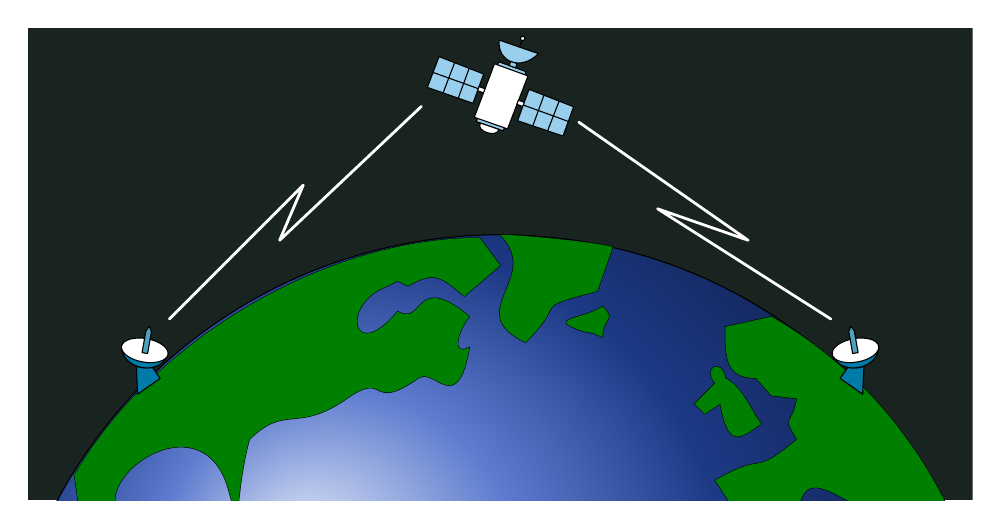
\begin{tikzpicture}[line join=round, line cap=round,scale=1,transform shape]
		\clip(-6,-3) rectangle (6,3);
		%\fill[darkelectricblue] (-6,-3) rectangle (6,3);%trời xám
		\fill[darkjunglegreen] (-6,-3) rectangle (6,3);%trời đen
		
		\tikzset{tram_phat/.pic={
				\def\T{ 
					(-5.26,-1.2)--(-5.45,-1.5)--(-5.1,-1.5)--(-5.1,-1.33)..controls +(150:.1) and +(-50:.1) ..cycle;
				}
				\fill[cerulean] \T;
				\draw\T;
				\draw[fill=cerulean,rotate=-45](-3.1,-4.35)
				..controls +(-80:.3) and +(-100:.3) ..(-2.5,-4.35);
				\draw[fill=white,rotate=-45](-2.5,-4.35) arc (0:360:.3 cm and .15cm);
				\draw[fill=cerulean!70](-5.1,-1.1)--(-4.9,-.9)--(-4.83,-.88)--(-4.85,-.95)--(-5.05,-1.15)--cycle;
		}}
		\tikzset{ve_tinh/.pic={
				\draw[fill=lightcornflowerblue] (-.95,0)--(-2.05,1.07)--(-1.3,1.8)--(-.25,.7)--cycle
				(-.95,1.4)--(-1.67,.7) (-.6,1.05)--(-1.3,.35) (-1.68,1.42)--(-.6,.35) ;
				\draw[fill=white]
				(-.4,.25)--(-.55,.4)--(-.65,.3)--(-.5,.15)--cycle;
				\draw[fill=lightcornflowerblue]
				(.35,.85)--(1,.2)--(-.45,-1.2)--(-1.1,-.57)--cycle;
				\draw[fill=white](.2,.85)--(1,.05)--(-.3,-1.2)--(-1.1,-.42)--cycle;
				(0,.35)--(.5,-.1)--(-.15,-.75)--(-.6,-.27)--cycle;
				\draw[fill=white](.55,-.67)--(.4,-.52)--(.3,-.62)--(.45,-.77)--cycle;
				\draw[fill=lightcornflowerblue](.85,-.35)--(1.9,-1.45)--(1.2,-2.15)--(.1,-1.1)--cycle
				(.47,-.72)--(1.55,-1.8) (1.2,-.72)--(.47,-1.45)
				(1.55,-1.1)--(.82,-1.8)
				(.6,.6)--(.7,.7)--(.85,.55)--(.75,.45)--cycle
				(.65,1.47)--(1.6,.55)
				..controls +(-160:.8) and +(-120:.7) ..(.65,1.47)
				(1.15,1)--(1.3,1.15)
				;
				\draw[fill=white] (1.35,1.2) circle (2pt);
				\draw[fill=white] (-1,-.67)
				..controls +(-150:.3) and +(-130:.3) ..(-.55,-1.1)--cycle;
		}}
		%=======================================
		\tikzset{earth/.pic={
				\def\D{ 
					(0,0) circle(4.9cm);
					
				}
				\fill[ball color=ceruleanblue] \D;
				\draw\D;
				
				\def\N{ 
					(-.2,4.87)
					..controls +(180:1.52) and +(60:1.5) ..(-4.16,2.55) 
					..controls +(-80:.5) and +(160:.5) ..(-3.7,1.75) --(-3.8,1.55) 
					..controls +(-45:.5) and +(130:.5) ..(-3.45,1) 
					..controls +(-20:1) and +(135:1.9) ..(-3.1,-1) 
					..controls +(-100:.5) and +(85:.9) ..(-3,-2) 
					..controls +(-95:.5) and +(85:.7) ..(-3.1,-3) 
					..controls +(-75:.5) and +(155:.7) ..(-2.4,-4.25) --(-2.5,-3.45) 
					..controls +(65:1) and +(-125:1.5) ..(-1.4,-2.1)
					..controls +(15:1) and +(-140:1) ..(-.3,-.8)
					..controls +(40:.4) and +(-85:.6) ..(-1.3,.3)
					..controls +(95:.4) and +(-45:.6) ..(-2.6,1.2)
					..controls +(145:.4) and +(-75:1.2) ..(-3.5,1.5)
					..controls +(55:.4) and +(-135:.5) ..(-3.4,1.9)
					..controls +(45:.2) and +(-35:.2) ..(-3.65,2.1)
					..controls +(145:.6) and +(105:1) ..(-2.65,2.4)
					..controls +(-75:.5) and +(-105:.6) ..(-2.45,2.9)
					..controls +(45:.5) and +(-145:.6) ..(-1.5,3.3)
					..controls +(35:.5) and +(-145:.6) ..(-.8,3.5)
					..controls +(35:.2) and +(-100:.7) ..(-.3,3.8)
					..controls +(-150:.2) and +(-130:.2) ..(-.3,4.1)
					..controls +(140:.7) and +(-30:.3) ..(-1,4.15)
					..controls +(-130:.7) and +(-160:.5) ..(-1.1,4.4)--(-1,4.45)--(-.9,4.4)
					..controls +(30:.3) and +(140:.3) ..(-.35,4.3)--(0,4.6)--cycle
					;
				}
				\draw[black]\N;
				\fill[ao(english)] \N;
				
				\def\N{ 
					(2.65,4.1)
					..controls +(-30:3.4) and +(32:3.3) ..(2.8,-4) 
					..controls +(-148:.4) and +(-120:.3) ..(2.95,-3.1) 
					..controls +(120:.4) and +(-120:.5) ..(3.3,-2) 
					..controls +(120:.4) and +(-90:.6) ..(3.3,-.8) 
					..controls +(100:.2) and +(20:.1) ..(3.1,-.8) 
					..controls +(120:1) and +(-50:2) ..(1.5,0)
					..controls +(80:1) and +(-150:.6) ..(2,1.5) 
					..controls +(30:.6) and +(170:.8) ..(3.2,1.9) %(4,1.5) 
					..controls +(-10:.6) and +(180:.8) ..(4.5,1.45)
					..controls +(120:.6) and +(-50:.9) ..(3.9,2.1) 
					..controls +(-120:.2) and +(-50:.2) ..(3.6,2.2)
					..controls +(-120:.2) and +(-100:.2) ..(3.4,2.3)
					..controls +(150:.4) and +(85:.4) ..(2.9,2.1)
					..controls +(-160:.6) and +(-55:.6) ..(2.1,2.5)
					..controls +(30:.6) and +(-140:.6) ..(2.9,2.9)
					..controls +(120:.3) and +(-100:.3) ..(2.9,3.3)--(2.65,3.33)--(2.5,3.5)
					..controls +(180:.3) and +(-90:.3) ..(2.2,4)--cycle
					;
				}
				\draw[black]\N;
				\fill[ao(english)] \N;
				
				\def\N{ 
					(0,4.9)
					..controls +(0:.2) and +(165:.2) ..(1.1,4.78)--(.95,4.35) 
					..controls +(-165:.7) and +(45:.6) ..(.25,3.85)
					..controls +(155:.7) and +(-45:.6) ..cycle
					
					(.7,4)
					..controls +(155:.2) and +(-145:.2) ..(1,4.2)
					..controls +(-45:.2) and +(90:.2) ..(1,3.9)
					..controls +(155:.2) and +(-25:.2) ..cycle
					
					(2.2,3.5)
					..controls +(-30:.2) and +(125:.2) ..(2.55,3.05)
					..controls +(-150:.2) and +(-80:.5) ..(2.15,3.25)--(2,3.15)--(1.9,3.25)--(2.1,3.45)
					..controls +(130:.2) and +(100:.2) ..cycle
					
					(-3,2)
					..controls +(40:.2) and +(165:.8) ..(-2.2,2)
					..controls +(-40:.2) and +(-165:.8) ..cycle
					
					(-2.5,1.6)
					..controls +(40:.2) and +(140:.2) ..(-2,1.7)
					..controls +(-40:.2) and +(-140:.2) ..cycle
					;
				}
				\draw[black]\N;
				\fill[ao(english)] \N;
		}}
		
		%================================================
		\draw[white,line width=1] (-4.2,-.7)--(-2.5,1)--(-2.8,.3)--(-1,2) (4.2,-.7)--(2,.7)--(3.15,.3)--(1,1.8);
		\path (0,-6)pic[scale=1.3]{earth}
		(-1,2.7)pic[rotate=35,scale=1]{tram_phat}
		(1,2.7)pic[rotate=-35,scale=1,rotate=180,yscale=-1]{tram_phat}
		(0,2.2)pic[rotate=25,scale=.4]{ve_tinh};
	\end{tikzpicture}
\end{center}
\shortans{$0{,}32$}
\loigiai{
Ta có, độ dài quãng đường truyền tín hiệu\\
$T=OM+MA=\sqrt{x^2+y^2+35^2}+\sqrt{(30-x)^2+(40-y)^2+35^2}$\\
$\ge \sqrt{(x+30-x)^2+(y+40-y)^2+(35+35)^2}=10\sqrt{74}$ (nghìn kilomet)\\
Thời gian ít nhất để $A$ nhận được tín hiệu từ $O$ là $\dfrac{10\sqrt{74}}{270}\approx 0,32$ (s).
}
\end{bt}

\begin{bt}%[2H2V1-4]
% nguon: Archive/2024/San pham - To Latex Strong - Tex hoa Lop 12 moi - Dot 2 (Chuong 1 + 2 + 3)/San pham - To Latex Strong - Tex hoa Lop 12 moi - Dot 2 (Chuong 1 + 2 + 3)/Data/Chuong 2/Chan troi sang tao/To 4 - Dot 17 - Chuong 2 - On tap chuong - CTST - De 1.tex #593
%[Tổ 4 - Đợt 12 - Chương 2 - Ôn tập chương đề 1 - CTST]%[Đoàn Tiến Phát]
	Khi chuyển động trong không gian, máy bay luôn chịu tác động của bốn lực chính: lực đẩy của động cơ, lực cản của không khí, trọng lực và lực nâng khí động học. Lực cản của không khí ngược hướng với lực đẩy của động cơ và có độ lớn tỉ lệ thuận với bình phương vận tốc máy bay. Một chiếc máy bay tăng vận tốc từ $900$ km/h lên $920$ km/h, trong quá trình tăng tốc máy bay giữ nguyên hướng bay. Lực cản của không khí khi máy bay đạt vận tốc $900$ km/h và $920$ km/h lần lượt được biểu diễn bởi hai vectơ $\overrightarrow{F_1}$ và $\overrightarrow{F_2}$. Biết $\overrightarrow{F_1}=k \overrightarrow{F_2}$ với $k$ là một số thực dương nào đó. Tính giá trị của $k$ (làm tròn kết quả đến chữ số thập phân thứ hai).
	\begin{center}
		\begin{tikzpicture}
		\clip (-4.5,-2.5) rectangle (4.5,2.5);
		\fill[bottom color=white,top color=blue!90, middle color=white] (-4.5,-2.5) rectangle (4.5,2.5);
		\begin{pgfinterruptboundingbox}
			
			%Đuôi máy bay
			\def\D{  (-2,-.45)--(-2.36,.24)--(-2.2,.3)--(-1.35,-.25)--cycle
				;}
			\draw \D;
			\fill[brown!40!] \D;
			
			%Quạt máy bay
			\def\Q{  (.15,-.1)
				..controls +(-140:0.1) and +(140:0.1) .. (.2,-.35)--(.8,-.17)--(.7,.07)--cycle
				
				;}
			\draw \Q;
			\draw[xshift=.5cm] \Q;
			\fill[brown!40!,xshift=.5cm] \Q;
			%---------elip2
			\draw[rotate=-70,xshift=-.23cm,yshift=1.27cm] (.7,-.1) ellipse (.12cm and .07cm);
			
			%Thân máy bay
			\def\T{  (-2.1,-.5)
				..controls +(40:0) and +(-170:0.7) .. (2,.74)
				..controls +(-40:0) and +(170:0.3) .. (2.55,.7)
				..controls +(-150:0) and +(30:.65) .. (2.1,.3)
				..controls +(-150:0) and +(-18:1.25) .. (-2.1,-.6)
				..controls +(90:0) and +(-90:0) .. (-2.1,-.51)
				-- (-2.5,-.52)--cycle;
			}
			\draw \T;
			\fill[brown!70!] \T;
			%Cánh máy bay
			\def\C{  (.5,.05)
				..controls +(170:0) and +(-10:0) .. (-1.48,.12)
				..controls +(-80:0) and +(170:0.02) .. (-1.65,.3)
				..controls +(180:0) and +(0:0) .. (-1.77,.3)
				..controls +(-80:0) and +(110:0) .. (-1.64,.12)
				..controls +(-35:0) and +(145:0) .. (-.2,-.17)
				--cycle
				;}
			\draw \C;
			\fill[brown!40!] \C;
			%Quạt sau
			\fill[brown!40!] \Q;
			%---------------Véc-tơ
			\draw[->,color=green] (.2,0)--(.2,-1.5)node[right] {Trọng lực};
			\draw[->,color=black] (.2,0)--(.2,1.5) node[right] {Lực nâng};
			\draw[->,color=blue] (.2,-.05)--(2.9,0.8) node[above] {Lực đẩy};
			\draw[->,color=red] (.2,-.05)--(-2.9,-1.05) node[below] {Lực cản không khí};
			%----elip 1
			\draw[rotate=-70,xshift=-.4cm,yshift=.8cm] (.7,-.1) ellipse (.12cm and .07cm);
			%Ô cửa
			\draw (2.18,0.73)--(2.5,0.7)--(2.14,0.58)--cycle;
			\fill[brown!40!](2.18,0.73)--(2.51,0.71)--(2.14,0.57)--cycle;
			
		\end{pgfinterruptboundingbox}
	\end{tikzpicture}
	\end{center}
	\shortans{$0{,}96$}
	\loigiai{
		Vì trong quá trình máy bay tăng vận tốc từ $900$ km/h lên $920$ km/h máy bay giữ nguyên hướng bay nên vectơ $\overrightarrow{F_1}$ và $\overrightarrow{F_2}$ có cùng hướng. Do đó, $\overrightarrow{F_1}=k \overrightarrow{F_2}$ với $k$ là một số thực dương nào đó (1).\\
		Gọi $v_1, v_2$ lần lượt là vận tốc của chiếc máy bay khi đạt $900$ km/h và $920$ km/h.\\
		Suy ra $v_1=900$ km/h, $v_2=920$ km/h.\\
		Vì lực cản của không khí ngược hướng với lực đẩy của động cơ và có độ lớn tỉ lệ thuận với bình phương vận tốc máy bay nên 
		\[
		\dfrac{\left|\overrightarrow{F_1}\right|}{\left|\overrightarrow{F_2}\right|}=\dfrac{v_1^2}{v_2^2}=\dfrac{900^2}{920^2}=\dfrac{2025}{2116}.
		\]
		Do đó, $\left|\overrightarrow{F_1}\right|=\dfrac{2025}{2116}\left|\overrightarrow{F_2}\right|$ (2).\\
		Từ (1) và (2) ta có $\overrightarrow{F_1}=\dfrac{2025}{2116} \overrightarrow{F_2} \Rightarrow k=\dfrac{2025}{2116} \approx 0{,}96$.
	}
\end{bt}

\begin{bt}%[2H2H2-6]
% nguon: Archive/2024/San pham - To Latex Strong - Tex hoa Lop 12 moi - Dot 2 (Chuong 1 + 2 + 3)/San pham - To Latex Strong - Tex hoa Lop 12 moi - Dot 2 (Chuong 1 + 2 + 3)/Data/Chuong 2/Chan troi sang tao/To 4 - Dot 17 - Chuong 2 - On tap chuong - CTST - De 2.tex #601
%[Tổ 4 - Đợt 17 - Chương 2 - Đề 2 - CTST]%[Huỳnh Thanh Chí]
	Trong hệ trục tọa độ $(Oxyz)$, một thiết bị âm thanh được phát từ vị trí $A(1; 5; 8)$. Người ta dự định đặt một máy thu tín hiệu trên mặt phẳng $(Oxy)$. Biết máy thu đặt ở vị trí $M(a; b; c)$ sẽ nhận được tín hiệu sớm nhất. Khi đó $a+2b+3c$ bằng
	\shortans[]{$11$}
	\loigiai{Người ta đặt máy thu trên mặt phẳng $(Oxy)$ sao cho nhận được tín hiệu sớm nhất nên bài toán trở thành: Tìm $M\in(Oxy)$ sao cho $MA$ đạt giá trị nhỏ nhất khi và chỉ khi $M$ là hình chiếu vuông góc của $A$ lên mặt phẳng $(Oxy)$.\\ 
	Do đó $M(1; 5; 0)$.\\
	Vậy $a+2b+3c=1+2\cdot 5+3\cdot 0=11$.
	}
\end{bt}

\begin{bt}%[2H2V2-6]
% nguon: Archive/2024/San pham - To Latex Strong - Tex hoa Lop 12 moi - Dot 2 (Chuong 1 + 2 + 3)/San pham - To Latex Strong - Tex hoa Lop 12 moi - Dot 2 (Chuong 1 + 2 + 3)/Data/Chuong 2/Chan troi sang tao/To 4 - Dot 17 - Chuong 2 - On tap chuong - CTST - De 2.tex #602
%[Tổ 4 - Đợt 17 - Chương 2 - Đề 2 - CTST]%[Huỳnh Thanh Chí]
	\immini{Một bình cá cảnh có dạng một chỏm cầu được đặt trên một chân đế (tham khảo hình vẽ). Biết tổng khối lượng bể cá là $20$ kg, ba chân đế là ba cạnh bên của một hình chóp cụt đều có độ dài cạnh bên bằng $50$ cm, hai đáy có độ dài lần lượt là $30$ cm và $20$ cm. Biết gia tốc trọng trường bằng $10$ m/s$^2$, tính độ lớn lực tác dụng của bể cá lên từng chân đế (kết quả làm tròn đến hàng phần mười).}
	{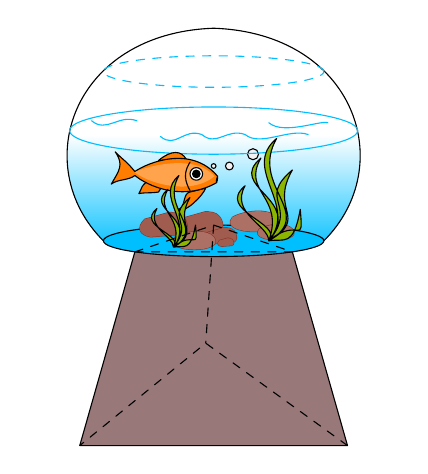
\begin{tikzpicture}[line join=round, line cap=round,scale=1,transform shape]
			\definecolor{applegreen}{rgb}{0.55, 0.71, 0.0}
			\definecolor{capri}{rgb}{0.0, 0.75, 1.0}
			\definecolor{amber}{rgb}{1.0, 0.49, 0.0}
			\definecolor{burntumber}{rgb}{0.54, 0.2, 0.14}
			\definecolor{aliceblue}{rgb}{0.94, 0.97, 1.0}
			\definecolor{anti-flashwhite}{rgb}{0.95, 0.95, 0.96}
			\definecolor{bazaar}{rgb}{0.6, 0.47, 0.48}
			\path (-1,-.54) coordinate (A)
			(1,-.54) coordinate (B)
			(1.7,-3) coordinate (C)
			(-1.7,-3) coordinate (D)
			;
			\draw[fill=bazaar] (B)--(C)--(D)--(A);
			
			\tikzset{rong/.pic={
					%=========Vẽ rong
					\def\R{ 
						(.7,-.4)
						..controls +(50:.6) and +(-140:.6) ..(1,.5)..controls +(-120:.6) and +(30:.6) ..cycle
						
						(.7,-.4)
						..controls +(50:.6) and +(-140:.6)..(.8,.9)..controls +(-120:.7) and +(30:.7) ..cycle
						
						(.7,-.4)
						..controls +(50:.7) and +(-140:.58)..(.6,.65)..controls +(-120:.5) and +(70:.6) ..cycle
						
						(.7,-.4)
						..controls +(50:.3) and +(-140:.5)..(.4,.3)..controls +(-120:.4) and +(90:.2) ..cycle
						
						(.7,-.4)
						..controls +(40:.5) and +(-85:.5)..(1.1,0)..controls +(-100:.5) and +(10:.2) ..cycle
						;
					}
					
					\fill[applegreen] \R;
					\draw\R;
			}}
			
			\tikzset{be/.pic={
					%----------------
					\def\M{ 
						(0,2.4)
						..controls +(-178:1.8) and +(135:1.35) ..(-1.4,-.3)--(1.4,-.3)
						..controls +(45:1.35) and +(-2:1.8) ..cycle
						;
					}
					
					\fill[bottom color=capri!90,top color=white, middle color=white] \M;
					%\fill[aliceblue]\M;
					\draw[black]\M;
					\draw[fill=capri] (1.4,-.3)  arc (0:360:1.4 cm and .2cm);
					
					
					\draw[dashed,color=capri] (1.4,1.85)  arc (0:360:1.4 cm and .2cm);
					\draw[fill=anti-flashwhite] (0,.65) circle (.03) ;
					\draw[fill=anti-flashwhite] (.2,.65) circle (.05) ;
					\draw[fill=anti-flashwhite] (.5,.8) circle (.07) ;
					
					\draw[capri] (1.83,1.1)  arc (0:360:1.83 cm and .3cm);
					%===========Vẽ cá
					%vây
					\def\V{ 
						(-.35,.74)
						..controls +(120:.12) and +(40:.22) ..(-.7,.72)--cycle
						(-.7,.32)
						..controls +(-170:.1) and +(10:.1) ..(-.95,.3)
						..controls +(60:.1) and +(-140:.1) ..(-.85,.45)--(-.65,.4)--cycle
						(-.3,.32)
						..controls +(-170:.1) and +(10:.1) ..(-.45,.1)
						..controls +(-40:.1) and +(-110:.1) ..(-.1,.37)--cycle
						;
					}
					\fill[amber] \V;
					\draw\V;
					
					%-----------------
					\def\C{ 
						(-1.25,.83)
						..controls +(-45:.2) and +(130:.2) ..(-1,.58)
						..controls +(35:.2) and +(130:.52) ..(.05,.52)
						..controls +(-90:.1) and +(-110:.1) ..(.05,.52)--(.04,.44)
						..controls +(-150:.5) and +(-40:.2) ..(-1,.53)
						..controls +(-140:.1) and +(40:.1) ..(-1.3,.42)
						..controls +(60:.2) and +(-55:.2) ..cycle
						;
					}
					
					\fill[amber] \C;
					\draw\C;
					%-----------------
					\def\Cn{ 
						(-1,.57)
						..controls +(35:.1) and +(130:.4) ..(.01,.52)
						..controls +(-140:.4) and +(-40:.2) ..cycle
						;
					}
					%\draw[ecru!70!black]\Cn;
					\fill[amber!70] \Cn;
					\draw (-.3,.7)
					..controls +(-120:.1) and +(120:.2) ..(-.3,.34);
					
					\draw[fill=white] (-.22,.55) circle (.08);
					\draw[fill=black] (-.22,.55) circle (.048);
					
			}}
			%----------------
			\tikzset{song/.pic={
					\def\S{ %sóng
						(-1.35,-2.15)
						..controls +(160:.5) and +(-40:.5) ..(-2.5,-2.15)
						(3.5,-2.2)
						..controls +(160:.2) and +(-40:.5) ..(2,-2.2)
						%----
						(3,-2.5)
						..controls +(160:.5) and +(-40:.5) ..(1.4,-2.5)
						..controls +(160:.5) and +(-40:.5) ..(.3,-2.5)
						..controls +(160:.5) and +(-40:.5) ..(-.75,-2.55)
						;}
					\draw[capri] \S;
			}}
			\tikzset{da2/.pic={
					\def\D2{ 
						(-.35,0)
						..controls +(30:.1) and +(130:.1) ..(0,0)
						..controls +(-50:.2) and +(-130:.2) ..cycle
						;
					}
					\draw[burntumber]\D2;
					\fill[burntumber!70] \D2;
			}}
			\tikzset{da1/.pic={
					\def\D1{ 
						(-.55,-1.28)
						..controls +(0:.1) and +(-10:.1) ..(-.58,-1.1)
						..controls +(175:.1) and +(15:.3) ..(-.85,-1.15)
						..controls +(-135:.1) and +(170:.1) ..(-.8,-1.3)--cycle
						;
					}
					\draw[burntumber]\D1;
					\fill[burntumber!80] \D1;
			}}
			\path
			(0,-.1)pic[scale=1]{be}
			(.8,-.1)pic[scale=1.6]{da2}
			(.8,1.5)pic[scale=1.4]{da1}
			(.4,1.6)pic[scale=1.5]{da1}
			(.78,.86)pic[scale=1]{da1}
			(.5,.18)pic[scale=.5]{da1}
			(0,-.35)pic[scale=1.4]{da2}
			(1,-.25)pic[scale=1.2]{da2}
			(-1,-.2) pic[scale=.7]{rong}
			(0,0)pic[scale=1]{rong}
			(-.3,2.2)pic[scale=.5]{song}
			;
			
			\path (-1,-.54) coordinate (A)
			
			(1,-.54) coordinate (B)
			(1.7,-3) coordinate (C)
			(-1.7,-3) coordinate (D)
			(0,-.2) coordinate (H)
			(-.1,-1.7) coordinate (K)
			;
			\draw[dashed] (A)--(B)--(H)--cycle (H)--(K) (C)--(K)--(D);
			
	\end{tikzpicture}}
	\shortans[]{$67{,}1$}
	\loigiai{Trọng lực của bể cá là $20\cdot 10=200$ N. \\
		Đổi $50$ cm bằng $5$ m, $30$ cm bằng $3$ m, $20$ cm bằng $2$ m.\\
		Kéo dài các cạnh bên của hình chóp cụt đều, ta được khối chóp tam giác đều $O.ABC$ (Hình vẽ bên dưới).
		\begin{center}		
		\begin{tikzpicture}[scale=1,font=\footnotesize,line join=round,line cap=round,>=stealth]
		\def\a{5}
		\def\h{3}
		\path 	(0:0) coordinate (A)
				++(0:\a) coordinate (C)
				++(-150:4*\a/5) coordinate (B)
				($(A)!0.5!(C)$) coordinate (Q)
				($(B)!2/3!(Q)$) coordinate (H)
				($(H)+(90:\h)$) coordinate (O)
				($(O)!0.6!(A)$) coordinate (M)
				($(O)!0.6!(B)$) coordinate (N)
				($(O)!0.6!(C)$) coordinate (P)
				($(B)!0.5!(A)$) coordinate (D)
				($(C)!2/3!(D)$) coordinate (G)
%				($(O)!2!(D)$) coordinate (E)
%				($(E)-(O)+(C)$) coordinate (F)
				;
		\draw (B)--(A) (C)--(B) (O)--(D) (A)--(O)	(B)--(O)	(C)--(O) (M)--(N)--(P);
		\draw[dashed] (A)--(C) (O)--(G) 	(P)--(M) (D)--(C);
		\foreach \x / \goc in {A/180,B/-90,C/45,M/135,O/90,N/-135,P/45,D/-180,G/45}
			\fill (\x) circle (1.0pt)
			($(\x)+(\goc:3mm)$) node {$\x$};
	\end{tikzpicture}
		\end{center}
		Gọi $F$ là độ lớn lực tác dụng lên từng chân đế.\\
		Gọi các vectơ lực của bể cá tác dụng lên các chân đến là $\overrightarrow{F}_1$, $\overrightarrow{F}_2$, $\overrightarrow{F}_3$.\\
		Vì vật đứng yên nên $\overrightarrow{F}_1+\overrightarrow{F}_2+\overrightarrow{F}_3=\overrightarrow{P}$.\\
		Ta có $F_1=F=\dfrac{F}{OA}\cdot OA$ suy ra $\overrightarrow{F}_1=\dfrac{F}{OA}\cdot \overrightarrow{OA}$.\\
		Tương tự $\overrightarrow{F}_2=\dfrac{F}{OB}\cdot \overrightarrow{OB}$, $\overrightarrow{F}_3=\dfrac{F}{OC}\cdot \overrightarrow{OC}$.\\
		Vì $O.ABC$ là hình chóp tam giác đều nên $OA=OB=OC$ nên $\overrightarrow{F}_1+\overrightarrow{F}_2+\overrightarrow{F}_3=\dfrac{F}{OA}\cdot\left(\overrightarrow{OA}+\overrightarrow{OB}+\overrightarrow{OC}\right)$.\\
		Khi đó $\overrightarrow{P}=\dfrac{F}{OA}\cdot\left(\overrightarrow{OA}+\overrightarrow{OB}+\overrightarrow{OC}\right)$.\\
		Gọi $G$ là trọng tam giác $ABC$, vì $O.ABC$ là hình chóp tam giác đều nên $3\overrightarrow{OG}=\overrightarrow{OA}+\overrightarrow{OB}+\overrightarrow{OC}$.\\
		Vậy $P=\dfrac{F}{OA}\cdot\left|\overrightarrow{OA}+\overrightarrow{OB}+\overrightarrow{OC}\right|=\dfrac{F}{OA}\cdot \left|3\overrightarrow{OG}\right|=\dfrac{F}{OA}\cdot 3OG$.\\
		Xét tam giác $OAB$ cân tại $O$ có $MN\parallel AB$ nên $\dfrac{OM}{OA}=\dfrac{MN}{AB}$ hay $\dfrac{OM}{OM+5}=\dfrac{2}{3}$, suy ra $OM=10$.\\
		Do đó $OA=OB=OC=15$.\\
		Gọi $D$ là trung điểm $AB$, khi đó $CD$ là đường cao của tam giác đều $ABC$.\\
		Khi đó $CG=\dfrac{2}{3}CD=\dfrac{2}{3}\cdot \dfrac{3\sqrt{3}}{2}=\sqrt{3}$. \\
		Xét tam giác $OCG$ vuông tại $G$, $OG=\sqrt{OC^2-CG^2}=\sqrt{15^2-\left(\sqrt{3}\right)^2}=\sqrt{222}$.\\
		Ta có $P=\dfrac{F}{OA}\cdot 3OG$ suy ra $F=\dfrac{OA\cdot P}{3OG}=\dfrac{15\cdot 200}{3\cdot \sqrt{222}}\approx 67{,}1$ N.	
	}
\end{bt}

\begin{bt}%[2H2C2-6]
% nguon: Archive/2024/San pham - To Latex Strong - Tex hoa Lop 12 moi - Dot 2 (Chuong 1 + 2 + 3)/San pham - To Latex Strong - Tex hoa Lop 12 moi - Dot 2 (Chuong 1 + 2 + 3)/Data/Chuong 2/Chan troi sang tao/To 4 - Dot 17 - Chuong 2 - On tap chuong - CTST - De 2.tex #603
%[Tổ 4 - Đợt 17 - Chương 2 - Đề 2 - CTST]%[Huỳnh Thanh Chí]
	\immini{Một mô hình trang trí có dạng là hình lập phương $ABCD.A'B'C'D'$ cạnh $4$ dm (như hình vẽ). Người ta cần nối một đường dây điện đi từ điểm $E$ (là trung điểm của $CD$) đi qua điểm $M$ thuộc cạnh $AD$, điểm $N$ thuộc cạnh $AA'$ tới $B'$. Độ dài đoạn dây điện ngắn nhất bằng bao nhiêu?}
	{\begin{tikzpicture}[scale=0.9,font=\footnotesize,line join=round,line cap=round,>=stealth]
			\def\a{3.5}
			\path 	(0:0) coordinate (A)
			++(0:\a) coordinate (D)
			++(-130:\a/2) coordinate (C)
			($(A)+(C)-(D)$) coordinate (B)
			($(A)+(90:\a)$) coordinate (A')
			($(B)+(90:\a)$) coordinate (B')
			($(C)+(90:\a)$) coordinate (C')
			($(D)+(90:\a)$) coordinate (D')
			($(C)!0.5!(D)$) coordinate (E)
			($(A)!1/3!(D)$) coordinate (M)
			($(A)!0.4!(A')$) coordinate (N)
			;
			\draw[dashed] 	(B)--(A)--(D)	(A)--(A') (E)--(M)--(N)--(B');
			\draw 	(C)--(C') 	(D)--(D') 	(B)--(B') 	(B)--(C)--(D) (A')--(B')--(C')--(D')--cycle;
			\foreach \x/\g in {A/180,B/180,C/0,D/0,A'/180,B'/180,C'/0,D'/0,E/-45,M/45,N/45}
			\fill 	(\x) circle (1pt)
			($(\g:4mm)+(\x)$) node {$\x$};	
	\end{tikzpicture}}
	\shortans[]{$10$}
	\loigiai{
	\begin{center}
		\begin{tikzpicture}[scale=1,font=\footnotesize,line join=round,line cap=round,>=stealth]
			\def\a{3.5}
			\path 	(0:0) coordinate (A)
			++(0:\a) coordinate (D)
			++(-130:\a/2) coordinate (C)
			($(A)+(C)-(D)$) coordinate (B)
			($(A)+(90:\a)$) coordinate (A')
			($(B)+(90:\a)$) coordinate (B')
			($(C)+(90:\a)$) coordinate (C')
			($(D)+(90:\a)$) coordinate (D')
			($(C)!0.5!(D)$) coordinate (E)
			($(A)!1/3!(D)$) coordinate (M)
			($(A)!0.4!(A')$) coordinate (N)
			;
			\draw[->] (A')--($(A')+(0,1.5)$)node[right]{$z$};
			\draw[->] (D)--($(D)+(1.5,0)$)node[above]{$y$};
			\draw[->] (B)--($(B)+(-130:1)$)node[left]{$x$};
			\draw[dashed] 	(B)--(A)--(D)	(A)--(A') (E)--(M)--(N)--(B');
			\draw 	(C)--(C') 	(D)--(D') 	(B)--(B') 	(B)--(C)--(D) (A')--(B')--(C')--(D')--cycle;
			\foreach \x/\g in {A/180,B/180,C/0,D/45,A'/180,B'/180,C'/0,D'/0,E/-45,M/45,N/45}
			\fill 	(\x) circle (1pt)
			($(\g:4mm)+(\x)$) node {$\x$};	
		\end{tikzpicture}
	\end{center}	
		Chọn hệ toạ độ $Oxyz$ sao cho $O$ trùng với $A$; các tia $Ox$, $Oy$, $Oz$ lần lượt trùng với các tia $AB$, $AD$ và $AA'$. \\
		Ta có $B'(4; 0; 4)$ và $E(2; 4; 0)$.\\
		Vì $N\in Oz \Rightarrow N(0; 0; a)$; $M\in Oy \Rightarrow M(0; b; 0)$ (điều kiện $0\leq a, b \leq 4$).\\
		Suy ra $B'N=\sqrt{16+(a-4)^2}$; $MN=\sqrt{a^2+b^2}$; $ME=\sqrt{4+(b-4)^2}$.\\
		Áp dụng bất đẳng thức Mincôpxki, ta có 
		\allowdisplaybreaks
		\begin{eqnarray*}
			B'N+MN+ME&=&\sqrt{16+(a-4)^2}+\sqrt{a^2+b^2}+\sqrt{4+(b-4)^2}\\
			&=&\sqrt{(4-a)^2+4^2}+\sqrt{a^2+b^2}+\sqrt{2^2+(4-b)^2} \\
			&\geq& \sqrt{(4-a+a+2)^2+(4+b+4-b)^2}\\
			&=&10.
		\end{eqnarray*}
		Dấu \lq\lq $=$ \rq\rq\ xảy ra khi $\dfrac{4-a}{4}=\dfrac{a}{b}=\dfrac{2}{4-b}=\dfrac{4-a+a+2}{4+b+4-b}=\dfrac{6}{8} \Rightarrow a=1; b=\dfrac{4}{3}$ (thoả mãn điều kiện).\\
		Vậy độ dài đoạn dây điện ngắn nhất bằng $10$ dm.
	}
\end{bt}

\begin{bt}%[2H2V2-6]
% nguon: Archive/2024/San pham - To Latex Strong - Tex hoa Lop 12 moi - Dot 2 (Chuong 1 + 2 + 3)/San pham - To Latex Strong - Tex hoa Lop 12 moi - Dot 2 (Chuong 1 + 2 + 3)/Data/Chuong 2/Chan troi sang tao/To 4 - Dot 17 - Chuong 2 - On tap chuong - CTST - De 3.tex #609
 %[Tổ Latex - Strong]%[Tổ 4 - Đợt 17 - Chương 2 - Ôn tập chương - CTST - Đề 3]%[Nguyễn Thắng]
Theo định luật II Newton, gia tốc của một vật có cùng hướng với lực tác dụng lên vật. Độ lớn của gia tốc tỉ lệ thuận với độ lớn của lực và tỉ lệ nghịch với khối lượng của vật $\overrightarrow{F}=m \cdot \overrightarrow{a}$, trong đó $\overrightarrow{a}$ là vectơ gia tốc $\left(m / s^2\right), \overrightarrow{F}$ là vectơ lực $(N)$ tác dụng lên vật, $m(\mathrm{~kg})$ là khối lượng của vật.\\
Muốn truyền cho quả bóng golf có khối lượng $0{,}046 \mathrm{~kg}$ một gia tốc $70 \mathrm{~m} / \mathrm{s}^2$ thì cần một lực đánh có độ lớn là bao nhiêu?\\
	\definecolor{ecru}{rgb}{0.76, 0.7, 0.5}
	\definecolor{dimgray}{rgb}{0.41, 0.41, 0.41}%màu quần
	\definecolor{cerisepink}{rgb}{0.93, 0.23, 0.51}
	\definecolor{burlywood}{rgb}{0.87, 0.72, 0.53}
	\definecolor{coral}{rgb}{1.0, 0.5, 0.31}%màu áo
	\definecolor{cobalt}{rgb}{0.0, 0.28, 0.67}
	\definecolor{otterbrown}{rgb}{0.4, 0.26, 0.13}
	\definecolor{gray(x11gray)}{rgb}{0.75, 0.75, 0.75}
	%------
	\definecolor{ecru}{rgb}{0.76, 0.7, 0.5}
	\definecolor{lightcornflowerblue}{rgb}{0.6, 0.81, 0.93}
	\definecolor{brightpink}{rgb}{1.0, 0.0, 0.5}
	\definecolor{ashgrey}{rgb}{0.7, 0.75, 0.71}
	
	\definecolor{green(ryb)}{rgb}{0.4, 0.69, 0.2}
	\definecolor{dollarbill}{rgb}{0.52, 0.73, 0.4}
	\definecolor{deepskyblue}{rgb}{0.0, 0.75, 1.0}
	\definecolor{fawn}{rgb}{0.9, 0.67, 0.44}
	%-------
	\definecolor{lightcornflowerblue}{rgb}{0.6, 0.81, 0.93}
	\definecolor{cadmiumgreen}{rgb}{0.0, 0.42, 0.24}
	\definecolor{trueblue}{rgb}{0.0, 0.45, 0.81}
	\definecolor{tumbleweed}{rgb}{0.87, 0.67, 0.53}%màu cát
	\definecolor{forestgreen(web)}{rgb}{0.13, 0.55, 0.13}
	\definecolor{darkpastelgreen}{rgb}{0.01, 0.75, 0.24}
	\definecolor{bronze}{rgb}{0.8, 0.5, 0.2}
	\definecolor{cadmiumgreen}{rgb}{0.0, 0.42, 0.24}
	
\begin{center}
	\begin{tikzpicture}[line join=round, line cap=round,scale=1,transform shape]
	\clip (-7.5,-3) rectangle (2,3);
	\tikzset{golf/.pic={
			\draw (3.2,3.92)
			..controls +(-70:.4) and +(-60:.4) ..(3.5,3.95)--cycle;
			\def\tay2{ 
				(-1.4,1.75)
				..controls +(120:.2) and +(-70:.3) ..(-1.65,2.2)
				..controls +(120:.2) and +(-100:.2) ..(-1.8,2.9)
				..controls +(95:.5) and +(170:.2) ..(-1.3,3.3)
				
				..controls +(10:.2) and +(160:.1) ..(-1,3.32)
				..controls +(-10:.2) and +(160:.1) ..(-1.2,2.8)
				..controls +(-60:.1) and +(160:.1) ..(-.9,2.38)
				..controls +(-40:.1) and +(40:.1) ..(-.7,1.8)--cycle
				;
			}
			%
			\fill[burlywood] \tay2;
			\draw[black]\tay2;
			\draw 
			(-1.3,3.1)
			..controls +(10:.15) and +(-110:.2) ..(-1,3.3);
			
			\def\tay{ 
				(-1.4,1.75)
				..controls +(120:.2) and +(-70:.3) ..(-1.65,2.2)
				..controls +(120:.2) and +(-100:.2) ..(-1.8,2.9)
				..controls +(95:.5) and +(170:.2) ..(-1.3,3.3)
				..controls +(-80:.2) and +(40:.1) ..(-1.5,2.9)
				..controls +(-80:.1) and +(130:.1) ..(-1.35,2.45)
				..controls +(-30:.1) and +(85:.1) ..(-1.15,2.2)
				;
			}
			\fill[burlywood] \tay;
			\draw[black]\tay;
			\draw[fill=gray(x11gray)] %gậy
			(-1.09,3.15)--(3.1,3.92)
			..controls +(-70:.65) and +(-60:.65) ..(3.5,4.02)
			..controls +(100:.1) and +(0:.6) ..(-1,3.28)--cycle;
			\def\ao{ 
				(-.2,2.55)
				..controls +(-10:1) and +(125:.9) ..(.6,.3)
				..controls +(-150:.3) and +(-35:.5) ..(-.8,.15)
				..controls +(120:.3) and +(-65:.5) ..(-1,1.4)
				..controls +(140:.2) and +(-55:.3) ..(-1.4,1.75)
				..controls +(85:.2) and +(-165:.3) ..(-1.15,2.25)
				..controls +(-35:.2) and +(-170:.2) ..(-.8,2.1)--cycle
				;
			}
			\fill[coral] \ao;
			\draw[black]\ao;
			\def\G{ 
				(-1.8,-3.9)
				..controls +(-80:.3) and +(90:.4) ..(-2.1,-4.4)--(-1.4,-4.4)
				..controls +(10:.1) and +(-40:.1) ..(-1.35,-4.1)--(-1.35,-3.9)--cycle
				(1.2,-3.9)
				..controls +(-80:.3) and +(90:.4) ..(1.6,-4.4)--(.79,-4.4)
				..controls +(140:.1) and +(-110:.1) ..(.82,-4.1)--(.82,-3.9)--cycle
				;
			}
			\fill[white] \G;
			\draw[black]\G;
			\def\Q{ 
				(.6,.3)
				..controls +(-150:.3) and +(-35:.5) ..(-.8,.15)
				..controls +(-120:.1) and +(95:.1) ..(-.92,-.15)
				..controls +(-80:.23) and +(95:.35) ..(-1.3,-1.5)
				..controls +(-110:.3) and +(85:.5) ..(-1.9,-3.9)
				..controls +(-30:.1) and +(120:.1) ..(-1.3,-4.15)
				..controls +(-95:.1) and +(-85:.2) ..(-.9,-2.4)
				..controls +(80:.1) and +(-150:.2) ..(-.1,-1)
				..controls +(-70:.1) and +(120:.2) ..(.27,-2)
				..controls +(-100:.1) and +(110:.2) ..(.8,-4.1)
				..controls +(-10:.1) and +(-170:.2) ..(1.3,-4)
				..controls +(130:.1) and +(-70:.2) ..(.95,-2)
				..controls +(110:.3) and +(-30:.5) ..cycle
				;
			}
			\fill[dimgray] \Q;
			\draw[black]\Q;
			\draw (-.1,-1)
			..controls +(-70:.1) and +(130:.1) ..(-.5,-.6);
			\draw (-.5,1.3)
			..controls +(-170:.1) and +(-30:.2) ..(-1,1.4);
			\def\toc{ 
				(-.6,2.45)
				..controls +(40:.1) and +(145:.1) ..(-.3,2.55)
				..controls +(70:.24) and +(45:.1) ..(-.25,2.45)
				..controls +(10:.1) and +(-100:.2) ..(-.2,2.8)
				..controls +(-150:.1) and +(50:.2) ..cycle
				;
			}
			\draw[black]\toc;
			\fill[black] \toc;
			\def\mat{ 
				(-.6,2.45)
				..controls +(40:.1) and +(145:.1) ..(-.3,2.55)
				..controls +(70:.24) and +(45:.1) ..(-.25,2.45)
				..controls +(20:.1) and +(20:.1) ..(-.1,2.3)
				..controls +(-160:.3) and +(50:.3) ..(-.5,2.1)
				..controls +(-130:.3) and +(-100:.5) ..(-1,2.7)
				;
			}
			\fill[burlywood] \mat;
			\draw[black]\mat;
			\def\N{ 
				(-.4,2.6)--(-.2,2.8)
				..controls +(95:.6) and +(95:.7) ..(-1.05,2.7)
				..controls +(-40:.1) and +(175:.1) ..cycle
				;
			}
			\draw[black]\N;
			\fill[cobalt] \N;
			\def\M{ 
				(-1.05,2.7)
				..controls +(-40:.1) and +(175:.1) .. (-.4,2.6)
				..controls +(-110:.2) and +(-45:.2) ..(-.8,2.43)
				..controls +(-35:.2) and +(35:.2) ..(-1.2,2.47)--cycle
				;
			}
			\draw[black]\M;
			\fill[cerisepink] \M;
			
			\draw (-.9,2.4)..controls +(80:.02) and +(90:.02) ..(-.83,2.41);
			\draw (-.74,2.19)..controls +(-50:.02) and +(-140:.02) ..(-.6,2.2);
	}}
	
	%%%%%%%%%%%%%%%%%%%%%% background
	\tikzset{ho/.pic={
			\def\D{ 
				(-6,-.7)
				..controls +(5:1.5) and +(-170:.7) ..(.8,-1.1)
				..controls +(10:1.2) and +(170:.7) ..(6,-.6)--(6,-6.5)--(-6,-6.5)--cycle
				;
			}
			\draw[green(ryb)]\D;
			\fill[green(ryb)] \D;
			
			\def\D1{ 
				(-6,-1.4)
				..controls +(20:1.5) and +(-170:.7) ..(.8,-1.15)
				..controls +(10:1.2) and +(170:.5) ..(6,-1.2)--(6,-6.5)--(-6,-6.5)--cycle
				;
			}
			\draw[dollarbill]\D1;
			\fill[dollarbill] \D1;
			
			\def\T{ 
				(-6,-.7)
				..controls +(5:1.5) and +(-170:.7) ..(.8,-1.1)
				..controls +(10:1.2) and +(170:.7) ..(6,-.6)--(6,3)--(-6,3)--cycle
				;
			}
			\draw[ecru!70!black]\T;
			\fill[bottom color=white,top color=deepskyblue!90, middle color=white] \T;
			
			\fill[green(ryb)] (6,-2.7)--(4,-2.4)
			..controls +(-170:.3) and +(30:.3) ..(2.5,-3.2)
			..controls +(-30:.3) and +(-170:.4) ..(4.8,-3.6)
			..controls +(10:.5) and +(-140:0) ..(6,-3.2)
			
			(-6,-2.2)--(-4.5,-1.8)
			..controls +(-20:.3) and +(140:.3) ..(-2.5,-2.2)
			..controls +(-30:.3) and +(-170:.4) ..(-4.8,-3)
			..controls +(10:.5) and +(-140:0) ..(-6,-2.5)
			
			(-6,-3.5)
			..controls +(-70:1) and +(110:.7) ..(-2,-4.5)
			..controls +(-70:1) and +(140:1) ..(2,-5.3)
			..controls +(-40:1) and +(-130:0) ..(6,-5)--(6,-6)--(-6,-6)--cycle
			;
			
			\def\tim{ 
				(0,-2)
				..controls +(160:1.4) and +(155:1.3) ..(2.2,-2)
				..controls +(-160:1.1) and +(-160:.8) ..cycle
				
				;
			}
			%\draw[fawn]\tim;
			\fill[fawn!80] \tim;
	}}
	%%%%%%%%%%%%%%%%%%%%bui cay
	\tikzset{cay/.pic={
			
			\def\C{ 
				(0,.3)
				..controls +(-100:.25) and +(-60:.2) ..  (-.3,.1)
				..controls +(-100:.25) and +(-60:.2) ..  (-.6,0)
				..controls +(-120:.45) and +(-110:.35) ..  (-1,.2)
				..controls +(-150:.5) and +(-140:.35) ..  (-1.15,.7)%nút giao
				..controls +(-170:.4) and +(-170:.35) ..  (-1,1.15)
				..controls +(140:.35) and +(110:.4) ..  (-.37,1.35)
				..controls +(110:.25) and +(80:.3) ..  (-.15,1.35)
				..controls +(80:.3) and +(95:.8) ..  (.55,1.1)
				..controls +(80:.2) and +(95:.2) ..  (.8,1.1)
				..controls +(20:.1) and +(95:.1) ..  (.95,1)
				..controls +(-20:.4) and +(35:.25) ..  (1,.47)
				..controls +(-30:.3) and +(-20:.3) ..  (.75,0.05)%nút giao
				..controls +(-120:.3) and +(-60:.2) ..  (.35,0)
				..controls +(175:.2) and +(-160:.1) ..  (.2,0.2)
				..controls +(-160:.1) and +(-70:.1) ..  (0,.3)
				;}
			\draw \C;
			\fill[forestgreen(web)] \C;
			\def\C1{ 
				(-1.15,.7)%nút giao
				..controls +(-170:.4) and +(-170:.35) ..  (-1,1.15)
				..controls +(140:.35) and +(110:.4) ..  (-.37,1.35)
				..controls +(110:.25) and +(80:.3) ..  (-.15,1.35)
				..controls +(80:.3) and +(95:.8) ..  (.55,1.1)
				..controls +(80:.2) and +(95:.2) ..  (.8,1.1)
				..controls +(20:.1) and +(95:.1) ..  (.95,1)
				..controls +(-20:.4) and +(35:.25) ..  (1,.47)
				..controls +(-50:.5) and +(-85:.6) ..  (.65,.55)% gần nút giao
				..controls +(-160:.4) and +(-120:.4) ..  (0,.7)
				..controls +(-150:.2) and +(-80:.4) ..  (-.63,.6)
				..controls +(-140:.5) and +(-130:.4) ..  (-1.15,.7)
				;}
			%\draw \C1;
			\fill[darkpastelgreen] \C1;
	}}
	%%%%%%%%%%%%%%%%%%%%
	\tikzset{cay2/.pic={%Cây
			\def\T{ 
				(-1.73,-2.85)
				..controls +(40:.03) and +(40:.01) ..  (-1.74,-2.7)
				..controls +(140:.04) and +(60:.02) ..  (-1.78,-2.6)
				..controls +(140:.04) and +(60:.02) ..  (-1.8,-2.55)
				..controls +(100:.03) and +(70:.02) ..  (-1.82,-2.5)
				..controls +(140:.04) and +(60:.02) ..  (-1.815,-2.4)
				..controls +(140:.04) and +(60:.02) ..  (-1.818,-2.3)
				..controls +(85:.03) and +(-30:.03) ..  (-1.8,-2.2)
				..controls +(80:.04) and +(50:.02) ..  (-1.78,-2)
				..controls +(60:.04) and +(120:.02) ..  (-1.76,-1.9)
				..controls +(80:.03) and +(-100:.02) ..  (-1.74,-1.8)
				..controls +(80:.01) and +(-100:.02) ..  (-1.72,-1.9)
				..controls +(60:.02) and +(-120:.02) ..  (-1.7,-2)
				..controls +(-80:.02) and +(110:.03) ..  (-1.66,-2.2)
				..controls +(-100:.02) and +(60:.03) ..  (-1.64,-2.3)
				..controls +(-30:.02) and +(70:.02) ..  (-1.6,-2.44)
				..controls +(-100:.02) and +(70:.02) ..  (-1.63,-2.52)
				..controls +(-60:.02) and +(70:.01) ..  (-1.66,-2.6)
				..controls +(60:.01) and +(70:.02) ..  (-1.7,-2.7)
				..controls +(-120:.02) and +(120:.03) ..  (-1.68,-2.85)
				;}
			\draw \T;
			\fill[cadmiumgreen!90!] \T;
	}}
	%%%%%%%%%%%%%%%%%%%%%%
	\path
	(0,4)pic[scale=1.5]{ho}
	(-6.6,-.5)pic[scale=.6]{cay}
	(-7,-.9)pic[scale=.5,rotate=5]{cay}
	(-2,0)pic[scale=.4,rotate=10]{cay}
	%(-4.2,7.3)pic[scale=1.7]{cay2}
	%(-4,8)pic[scale=2]{cay2}
	%(-4.8,8)pic[scale=2]{cay2}
	(-5,.1)pic[scale=.5]{golf}
	
	;
	
	\draw[fill=black] ($(5.5,-2.15)$) arc (0:360:.1cm and .05cm);
	\draw[thick] (5.5,-2.15)--(5.5,0);
	\draw[fill=red] (5.5,0)
	..controls +(-30:.2) and +(150:.2) ..(6,-.08)
	..controls +(-150:.5) and +(30:.2) ..(5.5,-.25)--cycle;
	
	\path 
	(-5.5,-2) coordinate (A)
	(-3.5,-1) coordinate (F)
	($(A)!.35!(F)$) coordinate (a)
	;
	\draw[dashed] (A)
	..controls +(30:3) and +(150:3) ..(5.3,-2.15);
	\draw[red,->] (A)--(F) node[below] {$\overrightarrow{F}$};
	\draw[blue,->] (A)--(a) node[below] {$\overrightarrow{a}$};
	\draw [fill=white] (-5.5,-2) circle (.1cm);
	\end{tikzpicture}
\end{center}
	\shortans{$3{,}22$}
	\loigiai{
		Ta có $\stackrel{\rightharpoonup}{F}=m \cdot \overrightarrow{a} \Rightarrow|\stackrel{\rightharpoonup}{F}|=m \cdot|\overrightarrow{a}|=0,046 \cdot 70=3{,}22$.}
\end{bt}

\begin{bt}%[2D1V3-6]
% nguon: Archive/2024/San pham - To Latex Strong - Tex hoa Lop 12 moi - Dot 2 (Chuong 1 + 2 + 3)/San pham - To Latex Strong - Tex hoa Lop 12 moi - Dot 2 (Chuong 1 + 2 + 3)/Data/Chuong 2/Chan troi sang tao/To 2 - Dot 17 - Chuong 2 - Bai 2 - CTST - De 1.tex #621 
% KIEM_TRA: cần xem lại đáp số/dạng
%[Tổ 2 - Đợt 17 - Chương 2 - Bài 2 - CTST - De 1]%[Nguyễn Hữu Duy]
	Người ta muốn chế tạo một chiếc hộp hình chữ nhật bằng tôn có nắp, có thể tích $400\, \mathrm{cm}^3$ với yêu cầu dùng ít vật liệu nhất. Biết chiều cao của hình hộp chữ nhật là $4\,\mathrm{cm}$. Chọn hệ trục tọa độ $Oxyz$ sao cho điểm $A$ trùng với gốc tọa độ $O$, vectơ $\overrightarrow{AB}$, $\overrightarrow{AD}$, $\overrightarrow{AA'}$ lần lượt cùng hướng với $\overrightarrow{i}$, $\overrightarrow{j}$, $\overrightarrow{k}$. Gọi $G(x;y;z)$ là trọng tâm của tam giác $A'BD$. Tính $3x + 2y + z$. 
	\shortans{$18$}
	\loigiai
	{
	\begin{center}
		\begin{tikzpicture}[scale=0.6, font=\footnotesize,line join=round, line cap=round, >=stealth]
			\path 
			(0,0) coordinate (A)node[above right]{$O$}
			++(-130:3) coordinate (B)
			++(0:6) coordinate (C)
			($(A)+(C)-(B)$) coordinate (D)
			($(A)!1/2!(C)$) coordinate (O)
			($(A)!1.5!(B)$) coordinate (E)
			($(D) + (0:1)$) coordinate (F)
			(0,5) coordinate (G)
			;
			\foreach \i in {A,B,C,D}{
				\coordinate (\i') at ($(\i)+(0,4)$);
			}
			\draw (A')--(B')--(C')--(D')--cycle;
			\draw[->] (B) -- (E) node[left]{$x$};
			\draw[->] (D) -- (F) node[right]{$y$};
			\draw[->] (A') -- (G) node[above]{$z$};

			\draw (B)--(B') (C)--(C') (D)--(D')  (B)--(C)--(D);
			\draw[dashed,thin](B)--(A)--(A') (A)--(D)--(B)--(A')--(D);
%			\pic[draw,angle eccentricity=1.8,angle radius=2mm]{right angle=B--O--C};
			\foreach \i/\g in {A'/150,B'/90,C'/90,D'/90,A/-90,B/-90,C/-90,D/-90}
			\fill[black] (\i) circle(1pt)+(\g:5mm)node[scale=1]{$\i$};
		\end{tikzpicture}
	\end{center}
	Gọi $x$, $y$ (cm, $x$, $y > 0$) là chiều dài và chiều rộng của hình chữ nhật $ABCD$.\\
	Theo giả thiết ta có $4xy = 400 \Leftrightarrow y = \dfrac{100}{x}$.\\
	Diện tich toàn phần của hình hộp chữ nhật là $S = 2\cdot 4x + 2 \cdot 4y + 2xy = 8x + \dfrac{800}{x} + 200$.\\
	Ta có $S = 8x + \dfrac{800}{x} + 200 \geq 2 \sqrt{8x \cdot \dfrac{800}{x}} + 200 = 360$.\\
	$S_{\text{min}} = 360 \Leftrightarrow 8x = \dfrac{800}{x} \Leftrightarrow x = 10 \Rightarrow y = 10$.\\
	Không mất tính tổng quát, chọn $B(10;0;0)$, $D(0;10;0)$; $A'(0;0;4)$.\\
	Do $G$ là trọng tâm tam giác $A'BD \Rightarrow G\left(\dfrac{10}{3};\dfrac{10}{3};\dfrac{4}{3}\right)$.\\
	Vậy $3x + 2y + z = \dfrac{54}{3} = 18$. 
 	}
\end{bt}

\begin{bt}%[2H2H2-6]
% nguon: Archive/2024/San pham - To Latex Strong - Tex hoa Lop 12 moi - Dot 2 (Chuong 1 + 2 + 3)/San pham - To Latex Strong - Tex hoa Lop 12 moi - Dot 2 (Chuong 1 + 2 + 3)/Data/Chuong 2/Chan troi sang tao/To 3 - Dot 17 - Chuong 2 - Bai 3 - CTST - De 1.tex #629
%[An Le]%[To3-Dot17-C2-Bai3-CTST-De1]%
	Trong không gian chọn hệ trục tọa độ cho trước, đơn vị đo lấy kilômét, ra đa phát 
	hiện một máy bay chiến đấu $X$ di chuyển với vận tốc và hướng không đổi từ điểm $M\left(1000;600;14 \right)$ đến điểm $N$ trong $30$ phút. Nếu máy bay tiếp tục giữ nguyên vận tốc và hướng bay thì tọa độ của máy bay sau $10$ phút tiếp theo bằng $Q\left(1400;800;16 \right)$. Tọa độ vị trí điểm $N\left(a;b;c \right)$, tính 
	$S=a+b+2c$.
	\shortans{$2081$}
	\loigiai{
		Gọi $N\left(x;y;z \right)$ là tọa độ của máy bay sau $30$ phút.\\ Ta có $\overrightarrow{MQ}=\left(400;200;2 \right)$,
		$\overrightarrow{NQ}=\left(1400-x;800-y;16-z \right)$.\\
		Vì máy bay giữ nguyên hướng bay nên $\overrightarrow{MQ}$ và $\overrightarrow{NQ}$ cùng hướng.\\
		Do máy bay tiếp tục giữ nguyên vận tốc và thời gian bay từ $M$ đến $Q$ gấp 4 lần thời gian bay từ 
		$N$ đến $Q$ nên $MQ=4NQ$.\\
		Suy ra $\overrightarrow{MQ}=4\overrightarrow{NQ}\Leftrightarrow\heva{& 400=4\left(1400-x \right) \\ 
			& 200=4\left(800-y \right) \\ 
			& 2=4\left(16-z \right)}\Leftrightarrow\heva{& x=1300 \\ 
			& y=750 \\ 
			& z=15,5.}$\\
			$\Rightarrow N\left(1300;750;15,5 \right)$.
	}
\end{bt}

\begin{bt}%[2H2V2-6]
% nguon: Archive/2024/San pham - To Latex Strong - Tex hoa Lop 12 moi - Dot 2 (Chuong 1 + 2 + 3)/San pham - To Latex Strong - Tex hoa Lop 12 moi - Dot 2 (Chuong 1 + 2 + 3)/Data/Chuong 2/Chan troi sang tao/To 2 - Dot 17 - Chuong 2 - Bai 2 - CTST - De 2.tex #649
%[Tổ 2 - Đợt 17 - Chương 2 - Bài 2 - CTST]%[Bùi Hà]
	Một sân cầu lông với kích thước theo tiêu chuẩn quốc tế là có chiều dài $13{,}40m$, chiều rộng là $6{,}10m$, chiều cao của lưới là $1{,}55m$. Ta chọn hệ trục $Oxyz$  cho sân đó sao cho gốc $O$ trùng với đỉnh một góc vuông của sân, mặt phẳng $(Oxy)$ trùng với mặt sân, trục $Oz$ vuông góc với mặt sân (đơn vị trên mỗi trục là mét). Giả sử $AA'$ là một trụ cầu lông để căng lưới. Biết tọa độ của vectơ $\overrightarrow{AA'}=(a;b;c)$ . Khi đó $S=a-b+2c$  bằng bao nhiêu?	\\
	\begin{center}
		
		\begin{tikzpicture}[scale=0.6, font=\footnotesize,line join=round, line cap=round, >=stealth]
			\path 
			(0,0) coordinate (O)
			++(-130:3) coordinate (B)
			++(0:6) coordinate (A)
			
			
			(-130:4) coordinate (E)
			($(D) + (0:1)$) coordinate (F)
			(0,5) coordinate (G)
			;
			\foreach \i in {O,A}{
				\coordinate (\i') at ($(\i)+(0,4)$);
			}
			
			\draw[->] (B) -- (E) node[left]{$x$};
			\draw[->] (D) -- (F) node[right]{$y$};
			\draw[->] (O) -- (G) node[above]{$z$};
			
			\draw   (O)--(D) (O)--(B) (A)--(A') ;
			
			%			\pic[draw,angle eccentricity=1.8,angle radius=2mm]{right angle=B--O--C};
			\foreach \i/\g in {O/-90,A/-90, A'/90}
			\fill[black] (\i) circle(1pt)+(\g:5mm)node[scale=1]{$\i$};
		\end{tikzpicture}
		
	\end{center}
	\shortans{3,1}
	\loigiai
	{ Vì véc-tơ $\overrightarrow{AA'}$ cùng hướng với véc-tơ đơn vị $\overrightarrow{k}$ của trục $Oz$ và $AA'=1{,}55$ nên $\overrightarrow{AA'}=1{,}55\overrightarrow{k}$. Do đó $\overrightarrow{AA'}=(0;0;1{,}55) \Rightarrow S=3{,}1$.
	}
\end{bt}

\begin{bt}%[2H2H2-6]
% nguon: Archive/2024/San pham - To Latex Strong - Tex hoa Lop 12 moi - Dot 2 (Chuong 1 + 2 + 3)/San pham - To Latex Strong - Tex hoa Lop 12 moi - Dot 2 (Chuong 1 + 2 + 3)/Data/Chuong 2/Chan troi sang tao/To 3 - Dot 17 - Chuong 2 - Bai 3 - CTST - De 3.tex #656
%[Tổ 3 - Đợt 17 - Chương 2 - Bài 3 - CTST]%[Phạm Tuấn]
Trên phần mềm mô phỏng việc điểu khiển drone giao hàng trong không gian $O x y z$, một drone giao hàng đang ở toạ độ $A(1 ; 0 ; 1)$ di chuyển đến địa điểm nhận hàng là $B(4 ; 4 ; 6)$. Mỗi đơn vị trên phần mềm bằng $1$ km ngoài thực tế. Biết tốc độ của drone là $80$ km/h; giả sử rằng từ vị trí giao hàng và nhận hàng không gặp chướng ngại vật, sức cản gió không đáng kể để drone bay theo đường thẳng. Thời gian drone bay từ vị trí ban đầu đến địa điểm giao hàng mất bao nhiêu phút (làm tròn đến hàng thập phân)?
\shortans{$5{,}3$}
\loigiai{
Tính được $A B=\sqrt{(4-1)^2+(4-0)^2+(6-1)^2}=5 \sqrt{2}$ (đơn vị trên phần mềm).\\
Do đó khoảng cách ngoài thực tế sẽ là $5 \sqrt{2}$ (km). \\
Thời gian bay của drone là $\dfrac{5 \sqrt{2}}{80}$ giờ, đổi sang bằng $\dfrac{5 \sqrt{2}}{80} \cdot 60=\dfrac{15 \sqrt{2}}{4} \approx 5{,}3$ phút.
}
\end{bt}

\begin{bt}%[2H2H2-6]
% nguon: Archive/2024/San pham - To Latex Strong - Tex hoa Lop 12 moi - Dot 2 (Chuong 1 + 2 + 3)/San pham - To Latex Strong - Tex hoa Lop 12 moi - Dot 2 (Chuong 1 + 2 + 3)/Data/Chuong 2/Chan troi sang tao/To 3 - Dot 17 - Chuong 2 - Bai 3 - CTST - De 3.tex #658
%[Tổ 3 - Đợt 17 - Chương 2 - Bài 3 - CTST]%[Phạm Tuấn]
Trong không gian với hệ trục tọa độ $O x y z$ cho trước, (đơn vị đo: km), ra đa phát hiện một máy bay chiến đấu Su-35 của Nga di chuyển với vận tốc và hướng không đổi từ điểm $M(300 ; 150 ; 7)$ đến điểm $N(800 ; 550 ; 13)$ trong $20$ phút. Gọi $P(a;b;c)$ là tọa độ của máy bay sau $5$ phút tiếp theo nếu máy bay giữ nguyên vận tốc và hướng bay. Tính $a+b-2c$.
\shortans{$1546$}
\loigiai{
Ta có $ \overrightarrow{M N}=(500 ; 400 ; 6)$. \\
Giả sử sau 5 phút, vị trí máy bay ở điểm $P$ thì $\overrightarrow{N P}=\dfrac{1}{4} \overrightarrow{M N}=\left(125 ; 100 ; \dfrac{3}{2}\right)$. \\
Do đó, tọa độ điểm $P$ là $\left(925 ; 650 ; \dfrac{29}{2}\right)$.\\
Suy ra $a+b-2c=1546$.
}
\end{bt}

\begin{bt}%[2H2V1-4]
% nguon: Archive/2024/San pham - To Latex Strong - Tex hoa Lop 12 moi - Dot 2 (Chuong 1 + 2 + 3)/San pham - To Latex Strong - Tex hoa Lop 12 moi - Dot 2 (Chuong 1 + 2 + 3)/Data/Chuong 2/Chan troi sang tao/To 1 - Dot 17 - Chuong 2 - Bai 1 - CTST - De 2.tex #667
%[Tổ 1 - Đợt 17 - Chương 2 - Bài 1 - CTST - Đề 2]%[Nguyễn Ngọc Dũng]
\immini{
Một chiếc đèn tròn được treo song song với mặt phẳng nằm ngang bởi ba sợi dây không giãn xuất phát từ điểm $O$ trên trần nhà và lần lượt buộc vào ba điểm $A$, $B$, $C$ trên đèn sao cho $OA$, $OB$, $OC$ đôi một vuông góc (như hình vẽ dưới đây). Biết khối lượng các sợi dây không đáng kể, các lực căng của sợi dây tai điểm $O$ là $\overrightarrow{F_1}$, $\overrightarrow{F_2}$, $\overrightarrow{F_3}$ có độ lớn bằng nhau và bằng $15$ N. Tính trọng lượng (đơn vị: N) của chiếc đèn đó (làm tròn kết quả đến hàng phần chục).
}{
\begin{tikzpicture}[line join=round, line cap=round, >=stealth, xscale=1, yscale=0.4, scale=0.9, font=\footnotesize]
\tikzset{label style/.style={font=\footnotesize}}
\path (0:0) coordinate (O')
++(0:2) coordinate (C)
($(O')+(150:2)$) coordinate (B)
($(O')+(220:2)$) coordinate (A)
($(O')+(90:8)$) coordinate (O)
($(O)!0.5!(A)$) coordinate (A1)
($(O)!0.5!(B)$) coordinate (B1)
($(O)!0.5!(C)$) coordinate (C1);
\draw[fill=blue,opacity=0.15] (O') circle (2 cm);
\draw (O') circle (2 cm);
\draw (O)--(A) (O)--(B) (O)--(C) (2,0)--(2,-1) (-2,0)--(-2,-1);
\draw (2,-1) arc (0:-180:2);
\draw[color=red,dashed] (C)--(O');
\draw[dashed] (O')--(0,-3);
\draw[fill=blue,opacity=0.4] (-2,8) rectangle (2,8.6);
\draw [->] (0,-3)--(0,-7)node[midway, right]{$\overrightarrow{P}$};
\draw [->] (O)--(A1)node[above right]{$\overrightarrow{F_1}$};
\draw [->] (O)--(B1)node[above left]{$\overrightarrow{F_2}$};
\draw [->] (O)--(C1)node[above right]{$\overrightarrow{F_3}$};
\draw (0,7.5) node[below] {$O$};
\foreach \x/\g in {A/60,B/100,C/0}
\fill (\x) circle (1pt)
($(\g:5mm)+(\x)$) node {$\x$};
\end{tikzpicture}
}
\shortans{$26$}
\loigiai{
\immini{
Gọi $P$ là trọng lượng của đèn, ta có 
$$P=\left|\overrightarrow{F_1}+\overrightarrow{F_2}+\overrightarrow{F_3}\right|=\left|\overrightarrow{OA}+\overrightarrow{OB}+\overrightarrow{OC}\right|.$$
Dựng hình hộp như hình vẽ bên. Khi đó, theo quy tắc hình hộp thì
$$P=\left|\overrightarrow{OA}+\overrightarrow{OB}+\overrightarrow{OC}\right|=\left|\overrightarrow{OF}\right|=OF.$$
Xét hình vuông $OAEB$, cạnh bằng $15$ nên $OE=15\sqrt{2}$.\\
Xét $\triangle OEF$ vuông tại $E$, có 
$$OF=\sqrt{OE^2+EF^2}=\sqrt{\left(15\sqrt{2}\right)^2+15^2}=15\sqrt{3}\approx 26.$$
Vậy $P\approx 26$ N.
}{
\begin{tikzpicture}[line join=round, line cap=round, font=\footnotesize, scale=1]
\def\a{3}
\path (0:0) coordinate (O)
++(0:\a) coordinate (B)
++(-160:\a*1.3) coordinate (A)
($(B)+(A)-(O)$) coordinate (E)
($(O)+(90:\a)$) coordinate (C)
($(E)+(90:\a)$) coordinate (F)
($(A)+(90:\a)$) coordinate (A')
($(B)+(90:\a)$) coordinate (B');
\draw[dashed] (O)--(A) (O)--(B) (O)--(C) (O)--(F) (O)--(E);
\draw (C)--(F) (C)--(A') (C)--(B') (F)--(E) (A)--(E)--(B)--(B')--(F)--(A')--cycle;
\foreach \x/\g in {O/170,A/-90,E/-90,B/-60,C/100,F/0}
\fill[black] (\x) circle (1pt)
($(\g:4mm)+(\x)$) node {$\x$}; 
\end{tikzpicture}
}
}
\end{bt}

\begin{bt}%[2H2V2-6]
% nguon: Archive/2024/San pham - To Latex Strong - Tex hoa Lop 12 moi - Dot 2 (Chuong 1 + 2 + 3)/San pham - To Latex Strong - Tex hoa Lop 12 moi - Dot 2 (Chuong 1 + 2 + 3)/Data/Chuong 2/Canh dieu/To 9 - Dot 16 - Chuong 2 - On tap chuong - CD - De 3.tex #687
%[Tổ 9-Đợt 16-Chương 2-Ôn tập chương-Cánh Diều]%[Duong Xuan Loi]
	Trong một căn phòng dạng hình hộp chữ nhật với chiều dài $8m$, rộng $6m$ và cao $4m$ có $2$ cây quạt treo tường. Cây quạt $A$ treo chính gữa bức tường $8m$ và cách trần $1m$, cây quạt $B$ treo chính giữa bức tường $6m$ và cách trần $1,5m$. Chọn hệ trục tọa độ $Oxyz$ như hình vẽ bên dưới (đơn vị: mét). Tọa độ của $\overrightarrow{AB}=(a;b;c)$. Hãy tính $a+b+c$?
	\begin{center}
			\definecolor{amber}{rgb}{1.0, 0.75, 0.0}%mau non
		\definecolor{antiquebrass}{rgb}{0.8, 0.58, 0.46}%mau da
		\definecolor{antiquewhite}{rgb}{0.98, 0.92, 0.84}%mau ao
		\definecolor{cadmiumgreen}{rgb}{0.0, 0.42, 0.24}%mau quan
		\definecolor{cadetblue}{rgb}{0.37, 0.62, 0.63}%mau but
		\definecolor{brown(traditional)}{rgb}{0.59, 0.29, 0.0}%mau giay
		\definecolor{brilliantlavender}{rgb}{0.96, 0.73, 1.0}%màu sơn tím
		\definecolor{brightube}{rgb}{0.82, 0.62, 0.91}%màu sơn tím đậm
		%---------------màu quạt 
		\definecolor{burntorange}{rgb}{0.8, 0.33, 0.0}
		\definecolor{arsenic}{rgb}{0.23, 0.27, 0.29}
		\definecolor{battleshipgrey}{rgb}{0.52, 0.52, 0.51}
		\begin{tikzpicture}[line join=round, line cap=round,scale=0.5,transform shape]
			\clip (1,-1) rectangle (16,13);
			%\draw[gray!50] (-3,-3) grid (3,4);
			
			\definecolor{burntsienna}{rgb}{0.91, 0.45, 0.32}                    
			\tikzset{mai/.pic={
					\def\mainha{ 
						(.5,2) 
						foreach \n in {1,2,...,22} { -- ++ (0,0) -- ++ (0,1) -- ++ (1,0) -- ++ (0,-1) } -- cycle
						
						(.5,1) 
						foreach \n in {1,2,...,22} { -- ++ (0,0) -- ++ (0,1) -- ++ (1,0) -- ++ (0,-1) } -- cycle
						
						(.5,0) 
						foreach \n in {1,2,...,22} { -- ++ (0,0) -- ++ (0,1) -- ++ (1,0) -- ++ (0,-1) } -- cycle
						
						(.5,-1) 
						foreach \n in {1,2,...,22} { -- ++ (0,0) -- ++ (0,1) -- ++ (1,0) -- ++ (0,-1) } -- cycle
						
						(.5,-2) 
						foreach \n in {1,2,...,22} { -- ++ (0,0) -- ++ (0,1) -- ++ (1,0) -- ++ (0,-1) } -- cycle
						
						(.5,-3) 
						foreach \n in {1,2,...,22} { -- ++ (0,0) -- ++ (0,1) -- ++ (1,0) -- ++ (0,-1) } -- cycle
						
						(.5,-4) 
						foreach \n in {1,2,...,22} { -- ++ (0,0) -- ++ (0,1) -- ++ (1,0) -- ++ (0,-1) } -- cycle
						;
					}
					\clip (-4,-3)--(17.5,-3)--(17.5,3)--(.5,3)--cycle;
					\draw[white,fill=burntsienna!70] \mainha;
					\draw (17.5,-3)--(17.5,3)--(17.5,9);
			}}
			
			\fill[brilliantlavender] (18,-3)--(18,13)--(12,13)--(12,-3)--cycle;
			\fill[brightube] (12,13)--(12,3)--(-18,3)--(-18,13)--cycle;
			\path
			(-2.5,0)pic[scale=1,xslant=-1]{mai}%
			;
			
			\path 
			(12,3) coordinate (O)
			(3,3) coordinate (x)
			(12,13) coordinate (z)
			(15,0) coordinate (y)
			;
			
			\foreach\p/\g in {y/160,x/45, z/-45,O/-90}
			{
				\node at (\p) [shift=(\g:4mm)] {$\p$};
			}	
			
			\draw[line width=.5mm,->] (O)--(z) ; 
			\draw[line width=.5mm,->] (O)--(x);
			\draw[line width=.5mm,->] (O)--(y);
			\node at ($(O)+(-6,4.5)$) {$8$ m};
			\draw[red,line width=.5mm,<->] ($(O)+(0,4)$)--($(x)+(-2,4)$);
			
			%===========================A FAN
			\tikzset{fan/.pic={
					%chân quạt
					\draw[fill=battleshipgrey](-.2,.8)--(.2,.8)--(.4,-2.2)
					..controls +(-120:.3) and +(-60:.3) ..(-.4,-2.2)--cycle;
					%---Nút bấm 
					\foreach \i in{-1.95,-1.7}{%-1.45
						\draw[fill=arsenic](-.15,\i) rectangle (.15,\i+.15);
					}
					%-----------------------------------------------------
					\draw[black](0,.8) circle (2.25cm);
					\draw[black](0,.8) circle (2.15cm);
					
					\draw[black](0,.8) circle (1.42cm);
					\draw[black](0,.8) circle (1.48cm);
					
					\draw[fill=black](0,.8) circle (6mm);
					\draw[fill=arsenic](0,.8) circle (5mm);
					\def\N{ 
						(0,.8)
						..controls +(145:1.3) and +(170:1) ..(0,2.8) 
						..controls +(-10:1.4) and +(-20:1) ..(.6,1.76) 
						..controls +(160:.4) and +(100:.4) ..(.2,.9)--cycle
						;
					}
					\foreach \i/\j/\k  in   {0/0/0,120/.7/-1.2,240/-.7/-1.2}
					{
						\draw[black,rotate=\i,shift={(\j,\k)}]\N;
						\fill[burntorange,rotate=\i,shift={(\j,\k)}] \N;
					}
					
					%lồng quạt
					\def\r{2.15}
					\foreach \i in {0,15,25,35,...,365}
					\draw[double] ($(\i:\r)+(0,.8)$)--(0,.8);
					
					\draw[fill=arsenic](0,.8) circle (3.5mm);					
					
			}}
			\path
			(6,11)pic[scale=.6]{fan}
			(14,9)pic[scale=.55,yslant=-.3]{fan};
		\end{tikzpicture}
	\end{center}
	\shortans{-1,5}
	\loigiai{
		Từ hình vẽ $A\in(Oxz)$ nên $A(x; 0; z)$, $B\in(Oyz)$ nên $B(0; y; z)$.\\
		Cây quạt $A$ treo chính giữa bức tường $8$m và cách trần $1m$ nên $A(4; 0; 3)$.\\
		Cây quạt $B$ treo chính giữa bức tường $6$m và cách trần $1{,}5$m nên $B\left(0; 3;\dfrac{5}{2}\right)$.\\
		Khi đó $\overrightarrow{AB}=\left(x_B-x_A;y_B-y_A;z_B-z_A\right)=\left(-4; 3;-\dfrac{1}{2}\right)$.\\
		Vậy $\heva{& a=-4 \\ & b=3\\&c=-\dfrac{1}{2}}\Rightarrow a+b+c=-1{,}5$.}
\end{bt}

\begin{bt}%[2H2V2-6]
% nguon: Archive/2024/San pham - To Latex Strong - Tex hoa Lop 12 moi - Dot 2 (Chuong 1 + 2 + 3)/San pham - To Latex Strong - Tex hoa Lop 12 moi - Dot 2 (Chuong 1 + 2 + 3)/Data/Chuong 2/Canh dieu/To 9 - Dot 16 - Chuong 2 - On tap chuong - CD - De 3.tex #688
%[Tổ 9-Đợt 16-Chương 2-Ôn tập chương-Cánh Diều]%[Duong Xuan Loi]
	Một chi tiết trong bộ trang sức có hình bát diện đều, được gắn hệ trục tọa độ $Oxyz$ như hình vẽ. Các hình chóp $S.ABCD$ và $I.ABCD$ là các hình chóp tứ giác đều cạnh $1 cm$. Số đo góc nhị diện $[S;CD;I]=a^\circ$ đơn vị độ, làm tròn đến hàng đơn vị. Khi đó $a$ bằng bao nhiêu?
	\begin{center}
		\begin{tikzpicture}[scale=1, font=\footnotesize, line join=round, line cap=round,>=stealth]
			\path
			(0,0) coordinate (A)
			(-1.9,-1.6)coordinate (B)
			(2.5,-1.6)coordinate (C)
			($(A)+(C)-(B)$)coordinate (D)
			($(A)!0.5!(C)$)coordinate (O)
			($(O)+(0,3.5)$) coordinate (S)
			($2*(O)-(S)$) coordinate (I)			
			;
			\draw (S)--(B)--(C)--(D)--cycle (S)--(C)--(I)--(B) (I)--(D);
			\draw[dashed] (A)--(I)--(S)--(A)--(D) (C)--(A)--(B)--(D);	
			\draw[->] (C)--($(O)!1.9!(C)$)node[above]{$x$};
			\draw[->] (D)--($(O)!1.9!(D)$)node[above]{$y$};
			\draw[->] (S)--($(O)!1.4!(S)$)node[right]{$z$};
			\fill (O) circle (1.0pt) node[right]{$O(0;0;0)$};
			\foreach \p/\q in {S/140,A/170,B/190,C/-75,D/-30,I/-90}
			\fill[black] (\p) circle (1.0pt)node[shift={(\q:3mm)}]{$\p$};	
		\end{tikzpicture}
	\end{center}
	\shortans{109}
	\loigiai{
		Ta có $OA=OB=OC=OD=\dfrac{\sqrt{2}}{2}$ nên $A\left(-\dfrac{1}{\sqrt{2}};0;0\right)$, $B\left(0;-\dfrac{1}{\sqrt{2}};0\right)$, $C\left(\dfrac{1}{\sqrt{2}};0;0\right)$,\\
		$D\left(0;\dfrac{1}{\sqrt{2}};0\right)$.\\
		Ta có $OI=SO=\sqrt{SA^2-OA^2}=\sqrt{1-\left(\dfrac{1}{\sqrt{2}}\right)^2}=\dfrac{1}{\sqrt{2}}$ nên $S\left(0;0;\dfrac{1}{\sqrt{2}}\right),I\left(0;0;-\dfrac{1}{\sqrt{2}}\right)$.\\
		Tổng hoành độ các đỉnh $S,A,B,C,D,I$ là 
		$-\dfrac{1}{\sqrt{2}}+0+\dfrac{1}{\sqrt{2}}+0+0+0=0$.\\	
		Gọi $M$ là trung điểm của $CD$ thì $M\left(\dfrac{1}{2\sqrt{2}};\dfrac{1}{2\sqrt{2}};0\right)$. 
		\begin{center}
			\begin{tikzpicture}[scale=1, font=\footnotesize, line join=round, line cap=round,>=stealth]
				\path
				(0,0) coordinate (A)
				(-1.9,-1.6)coordinate (B)
				(2.5,-1.6)coordinate (C)
				($(A)+(C)-(B)$)coordinate (D)
				($(A)!0.5!(C)$)coordinate (O)
				($(O)+(0,3.5)$) coordinate (S)
				($2*(O)-(S)$) coordinate (I)
				($(C)!0.5!(D)$) coordinate (M)							
				;
				\draw (S)--(B)--(C)--(D)--cycle (S)--(C)--(I)--(B) (S)--(M)--(I)--(D);
				\draw[dashed] (A)--(I)--(S)--(A)--(D) (C)--(A)--(B)--(D);	
				\draw[->] (C)--($(O)!1.9!(C)$)node[above]{$x$};
				\draw[->] (D)--($(O)!1.9!(D)$)node[above]{$y$};
				\draw[->] (S)--($(O)!1.4!(S)$)node[right]{$z$};
				\fill (O) circle (1.0pt) node[right]{$O(0;0;0)$};
				\foreach \p/\q in {S/140,A/170,B/190,C/-75,D/-30,I/-90,M/70}
				\fill[black] (\p) circle (1.0pt)node[shift={(\q:3mm)}]{$\p$};	
			\end{tikzpicture}
		\end{center}
		Có $\heva{&CD\perp OM\\&CD\perp SO}\Rightarrow[S;CD;I]=\widehat{SMI.}$ \\
		Ta có $\overrightarrow{MS}\left(-\dfrac{1}{2\sqrt{2}};-\dfrac{1}{2\sqrt{2}};\dfrac{1}{\sqrt{2}}\right),\overrightarrow{MI}\left(-\dfrac{1}{2\sqrt{2}};-\dfrac{1}{2\sqrt{2}};-\dfrac{1}{\sqrt{2}}\right)$.
		\begin{eqnarray*}
			\cos\widehat{SMI}&=&\dfrac{-\dfrac{1}{2\sqrt{2}}\cdot -\dfrac{1}{2\sqrt{2}}+-\dfrac{1}{2\sqrt{2}}\cdot -\dfrac{1}{2\sqrt{2}}+\dfrac{1}{\sqrt{2}}\cdot -\dfrac{1}{\sqrt{2}}}{\sqrt{\left(-\dfrac{1}{2\sqrt{2}}\right)^2+\left(-\dfrac{1}{2\sqrt{2}}\right)^2+\left(\dfrac{1}{\sqrt{2}}\right)^2}\cdot\sqrt{\left(-\dfrac{1}{2\sqrt{2}}\right)^2+\left(-\dfrac{1}{2\sqrt{2}}\right)^2+\left(\dfrac{-1}{\sqrt{2}}\right)^2}}\\
			&=&-\dfrac{1}{3}\\
			&\Rightarrow&\widehat{SMI}\approx 109^{\circ}.
		\end{eqnarray*}
		}
\end{bt}

\begin{bt}%[2H2V2-6]
% nguon: Archive/2024/San pham - To Latex Strong - Tex hoa Lop 12 moi - Dot 2 (Chuong 1 + 2 + 3)/San pham - To Latex Strong - Tex hoa Lop 12 moi - Dot 2 (Chuong 1 + 2 + 3)/Data/Chuong 2/Canh dieu/To 9 - Dot 16 - Chuong 2 - On tap chuong - CD - De 3.tex #689
%[Tổ 9-Đợt 16-Chương 2-Ôn tập chương-Cánh Diều]%[Duong Xuan Loi]
	Một chiếc ô tô được đặt trên mặt đáy dưới của một khung sắt có dạng hình hộp chữ nhật với đáy trên là hình chữ nhật $ABCD$, mặt phẳng $(ABCD)$ song song với mặt phẳng nằm ngang. Khung sắt đó được buộc vào móc $E$ của chiếc cần cẩu sao cho các đoạn dây cáp $EA, EB, EC$ và $ED$ có độ dài bằng nhau và cùng tạo với mặt phẳng $(ABCD)$ một góc bằng $60^{\circ}$ (hình minh họa). Chiếc cần cẩu đang kéo khung sắt lên theo phương thẳng đứng. 
	\begin{center}
		\begin{tikzpicture}[>=stealth,line join=round, line cap=round,scale=.7,transform shape]
			\definecolor{bostonuniversityred}{rgb}{0.8, 0.0, 0.0}
			\definecolor{charcoal}{rgb}{0.21, 0.27, 0.31}
			\definecolor{bananayellow}{rgb}{1.0, 0.88, 0.21}
			\definecolor{anti-flashwhite}{rgb}{0.95, 0.95, 0.96}
			%	\clip (-6,-3) rectangle (6,3);
			\tikzset{%
				xeoto/.pic={%
					%--------------------------	
					\tikzset{xe/.pic={
							\def\N{ 
								(-2.7,.56)--(-2.5,.56)
								..controls +(50:1.5) and +(165:1.5) .. (2.1,1.88)--(2.05,2)
								..controls +(-10:.1) and +(130:.1) .. (3.25,1.75)--(3.15,1.65)
								..controls +(-4:.2) and +(130:.15) .. (4.05,.7)--(4.25,.75)
								..controls +(-40:.2) and +(130:.15) .. (4.55,.35)--(4.35,.26)
								..controls +(-40:.2) and +(130:.15) .. (4.8,-.45)--(4.92,-.4)
								..controls +(-40:.25) and +(73:.17) .. (4.8,-1.8)--(-4.4,-1.8)
								..controls +(175:.7) and +(-175:3.2) ..cycle
								;
							}
							\fill[bostonuniversityred] \N;
							\draw \N;
							\def\K{ 
								(-2.2,.56)--(3.3,.7)
								..controls +(100:1.18) and +(43:3) .. cycle
								;
							}
							\fill[bottom color=charcoal,top color=charcoal!20!white, middle color=charcoal!80!white] \K;
							\draw \K;
							\def\K1{ 
								(-2.2,.56)
								..controls +(43:.2) and +(43:.2) .. (-1.58,1.05)--(-1.53,.57)--cycle
								;
							}
							\draw \K1;
							\fill[charcoal] \K1;
							\def\K2{ 
								(1.2,1.85)
								..controls +(-10:.1) and +(160:.1) .. (1.58,1.8)--(1.8,.65)--(1.25,.65)--cycle
								;
							}
							\draw \K2;
							\fill[charcoal] \K2;
							\def\Kt{ 
								(-2.5,.56)
								..controls +(50:1.5) and +(165:1.5) .. (2.1,1.88)--(2.05,2)
								..controls +(170:2.2) and +(45:1.5) .. (-2.7,.56)--cycle
								;
							}
							\fill[charcoal!50] \Kt;
							\draw \Kt;
							\def\Ks{ 
								(3.25,1.75)--(3.15,1.65)
								..controls +(-4:.2) and +(130:.15) .. (4.05,.7)--(4.22,.75)
								..controls +(120:.3) and +(-35:.3) .. cycle
								;
							}
							\fill[charcoal!50] \Ks;
							\draw \Ks;
							%Đèn sau
							\def\D{ 
								(4.55,.35)--(4.35,.26)
								..controls +(-40:.2) and +(130:.15) .. (4.8,-.45)--(4.92,-.4)
								..controls +(110:.2) and +(-40:.15) ..cycle
								;
							}
							\fill[bananayellow] \D;
							\draw \D;
							\def\M{ 
								(2.2,-1.3)--(-1.8,-1.4)--(-1.78,-1.7)
								..controls +(-5:.3) and +(-90:.6) ..cycle
								;
							}
							\draw \M;
							\fill[charcoal!90] \M;
							\draw (-1.6,.55)
							..controls +(-170:.5) and +(95:.4) .. (-1.78,-1.7)
							(1.6,.65)
							..controls +(-30:.5) and +(35:.3) .. (1.7,-1.3)
							;
							%gương
							\def\G{ 
								(-1.5,.45)--(-1.4,.6)
								..controls +(85:1) and +(20:.6) .. (-1.25,.5)--(-1.4,.33)
								;
							}
							\draw \G;
							\fill[bostonuniversityred] \G;
							%Đèn trước
							\def\Dt{ 
								(-4.85,-.7)
								..controls +(75:1) and +(65:.8) .. (-4.5,-.7)
								..controls +(-115:.6) and +(-105:.4) .. cycle
								;
							}
							\fill[bananayellow] \Dt;
							\draw \Dt;
							\def\Dt2{ 
								(-4.85,-.7)
								..controls +(75:.6) and +(65:.4) .. (-4.7,-.7)
								..controls +(-115:.3) and +(-105:.2) .. cycle
								;
							}
							\fill[anti-flashwhite] \Dt2;
							\draw \Dt2;
							\draw[fill=anti-flashwhite] (-4.86,-1.45)--(-4.82,-1.5)--(-4.55,-1.3)
							..controls +(90:.3) and +(45:.2) .. cycle;
					}}
					\tikzset{banh_xe/.pic={
							\draw[fill=charcoal] (-3.25,-1.65) circle (1) ;
							\draw[fill=anti-flashwhite] (-3.25,-1.65) circle (.7) ;
							\draw[fill=charcoal] (-3.25,-1.65) circle (.4) ;
					}}
					%----------------
					\path
					(0,0)pic[scale=1]{xe}(0,0)pic[scale=1]{banh_xe}(6.9,0)pic[scale=1]{banh_xe};
					%--------------------------------
			}}
			%%%%%%%%%%%%%%%%%%%
			\def\bc{4.25} % cạnh BC
			\def\ba{1.5} % cạnh BA
			\def\h{4} % đường cao
			\def\gocnghieng{90} % góc nghiêng
			\def\gocB{160} % góc B của đáy
			\coordinate (B1) at (0,0);
			\coordinate (A1) at (\gocB:\ba);
			\coordinate (C1) at (\bc,0.25);
			\coordinate (D1) at ($(C1)-(B1)+(A1)$);
			\coordinate[label=above left:$A$] (A) at ($(A1)+(\gocnghieng:\h)$);
			\coordinate[label=below left:$B$] (B) at ($(B1)-(A1)+(A)$);
			\coordinate[label=right:$C$] (C) at ($(C1)-(A1)+(A)$);
			\coordinate[label=above right:$D$] (D) at ($(D1)-(A1)+(A)$);
			\coordinate (E) at ($(A)!0.5!(C)+(\gocnghieng:\h)$);
			%------------
			\draw[->,blue,very thick] (E)--($(E)!0.6!(A)$) node[above left]{$\overrightarrow{F}_1$};
			\draw[->,blue,very thick] (E)--($(E)!0.6!(B)$) node[right]{$\overrightarrow{F}_2$};
			\draw[->,blue,very thick] (E)--($(E)!0.6!(C)$) node[above right]{$\overrightarrow{F}_3$};
			\draw[->,blue,very thick] (E)--($(E)!0.6!(D)$) node[left=2pt]{$\overrightarrow{F}_4$};
			%------------
			\path (E) node[left=1mm]{$E$};
			\draw[blue,very thick] (A)--(B)--(C)--(D)--cycle
			(A1)--(A) (D1)--(D) (C1)--(C)
			(A)--(E)--(B) (C)--(E)--(D);
			\draw[fill=teal] (A1)--(B1)--(C1)--(D1)--cycle;
			\draw[fill=teal!30] (A1)--(B1)--(C1)--++(0,-0.3)--([yshift=-0.3cm]B1)--([yshift=-0.3cm]A1)--cycle;
			\foreach \diem in {A1,B1,C1,D1,A,B,C,D,E}	\fill (\diem)circle(1.5pt);
			%phần móc và dây
			\def\r{0.3}\def\rr{0.25}
			\coordinate (tam) at ([yshift=6mm]E);
			\draw[brown,fill=brown,line width=1pt] (tam) circle (\r cm);
			\fill (tam) circle (2pt);
			\draw[brown,line width=1pt] (tam)++(\r,0)--++(0,0.7)
			(tam)++(-\r,0)--++(0,0.7);
			\draw[line width=1.5pt] (tam)--++(0,-1.35*\r) arc(90:370:1mm);
			%%%%%%%%%%%%%%%%%%%
			\pic[scale=0.45,rotate=4] at (1.6,1.3) [pic type = xeoto];
			%--------
			\draw[blue,very thick] (B)--(B1);
		\end{tikzpicture}
	\end{center}
	Biết rằng các lực căng $\overrightarrow{F}_1$,  $\overrightarrow{F}_2$, $\overrightarrow{F}_3$, $\overrightarrow{F}_4$ đều có cường độ là $4{,}7$kN và trọng lượng của khung sắt là $3$kN. Tính trọng lượng lớn nhất của chiếc xe ô tô (làm tròn đến hàng phần chục)?
	\shortans{13,3}
	\loigiai{
		\immini{
			Gọi $A_1,B_1,C_1$, $D_1$ lần lượt là các điểm sao cho.\\
		$\overrightarrow{EA}_1=\overrightarrow{F}_1$, $\overrightarrow{EB}_1=\overrightarrow{F}_2$, $\overrightarrow{EC}_1=\overrightarrow{F}_3$, $\overrightarrow{ED_1}=\overrightarrow{F}_4$.\\ 
		Vì $EA, EB,EC,ED$ có độ dài bằng nhau và cùng tạo với mặt phẳng ($ABCD$) một góc bằng $60^{\circ}$ nên $EA_1,EB_1,EC_1,ED_1$ bằng nhau và cùng tạo với mặt phẳng $\left(A_1B_1C_1D_1\right)$ một góc bằng $60^{\circ}$.\\
		Vì $ABCD$ là hình chữ nhật nên $A_1B_1C_1D_1$ cũng là hình chữ nhật. 
		}{
			\begin{tikzpicture}[scale=1, font=\footnotesize, line join=round, line cap=round,>=stealth]
				\path
				(0,0) coordinate (D_1)
				(-1.9,-1.6)coordinate (A_1)
				(1.6,-1.6)coordinate (B_1)
				($(B_1)+(D_1)-(A_1)$)coordinate (C_1)
				($(A_1)!0.5!(C_1)$)coordinate (O)
				($(O)+(0,3.5)$) coordinate (E)
				;
				\draw (A_1)--(B_1)--(C_1);
				\draw[dashed] (A_1)--(D_1)--(C_1)--cycle (D_1)--(B_1);	
				\draw[->] (E)--(A_1)node[above left,midway]{$\overrightarrow{F}_1$};
				\draw[->,dashed] (E)--(D_1)node[below left,midway]{$\overrightarrow{F}_4$};
				\draw[->] (E)--(B_1)node[right,midway]{$\overrightarrow{F}_2$};
				\draw[->] (E)--(C_1)node[above right,midway]{$\overrightarrow{F}_3$};
				\draw[->,dashed] (E)--(O);
				\foreach \p/\q in {E/90,A_1/-100,B_1/-90,C_1/0,D_1/170,O/-90}
				\fill[black] (\p) circle (1.0pt)node[shift={(\q:3mm)}]{$\p$};	
			\end{tikzpicture}
		}\noindent
		Gọi $O$ là tâm của hình chữ nhật $A_1B_1C_1D_1$. 
		Ta suy ra $EO\perp\left(A_1B_1C_1D_1\right)$.\\
		Do đó, góc giữa đường thẳng $EA_1$ và mặt phẳng $\left(A_1B_1C_1D_1\right)$ bằng góc $\widehat{EA_1O}$. \\
		Suy ra $\widehat{EA_1O}=60^{\circ}$.\\
		Ta có $\left|\overrightarrow{F}_1\right|=\left|\overrightarrow{F}_2\right|=\left|\overrightarrow{F}_3\right|=\left|\overrightarrow{F}_4\right|=4700$(N) nên $EA_1=EB_1=EC_1=ED_1=4{,}7$. \\
		Tam giác $EA_1O$ vuông tại $O$ nên $EO=EA_1\sin\widehat{EA_1O}=4{,}7\sin 60^{\circ}=2{,}35\sqrt{3}$. \\
		Theo quy tắc ba điểm, ta có $\overrightarrow{EA_1}=\overrightarrow{EO}+\overrightarrow{OA_1},\overrightarrow{EB_1}=\overrightarrow{EO}+\overrightarrow{OB_1},\overrightarrow{EC_1}=\overrightarrow{EO}+\overrightarrow{OC_1}$, $\overrightarrow{ED_1}=\overrightarrow{EO}+\overrightarrow{OD_1}$.\\
		Vì $O$ là trung điểm của $A_1C_1$ và $B_1D_1$ nên $\overrightarrow{OA_1}+\overrightarrow{OC_1}=\overrightarrow{0},\overrightarrow{OB_1}+\overrightarrow{OD_1}=\overrightarrow{0}$.\\
		Từ đó suy ra $\overrightarrow{EA_1}+\overrightarrow{EB_1}+\overrightarrow{EC_1}+\overrightarrow{ED_1}=4\overrightarrow{EO}$. \\
		Do đó, $\overrightarrow{F_1}+\overrightarrow{F_2}+\overrightarrow{F_3}+\overrightarrow{F_4}=4\overrightarrow{EO}$.\\
		Gọi $P$ là trọng lực của khung sắt có chứa chiếc ô tô.\\ 
		Vì chiếc khung sắt chứa xe ô tô đang được kéo lên. Suy ra trọng lượng của khung sắt chứa chiếc xe ô tô là $\left|\overrightarrow{P}\right|\leq 4\left|\overrightarrow{EO}\right|=4\cdot 2{,}35\sqrt{3}=9,4\sqrt{3}(kN)$.\\
		Vì trọng lượng của khung sắt là $3kN$ nên trọng lượng của chiếc xe ô tô là\\ $9,4\sqrt{3}-3\approx 13{,}3$ (kN).}
\end{bt}

\begin{bt}%[2H2V2-6]
% nguon: Archive/2024/San pham - To Latex Strong - Tex hoa Lop 12 moi - Dot 2 (Chuong 1 + 2 + 3)/San pham - To Latex Strong - Tex hoa Lop 12 moi - Dot 2 (Chuong 1 + 2 + 3)/Data/Chuong 2/Canh dieu/To 9 - Dot 16 - Chuong 2 - On tap chuong - CD - De 1.tex #702

	Trong không gian với một hệ trục toạ độ cho trước (đơn vị đo lấy theo kilômét), ra đa phát hiện một chiếc máy bay di chuyển với vận tốc và hướng không đổi từ điểm $A\left(800;500;7\right)$ đến điểm $B\left(940;550;9\right)$ trong 10 phút. Nếu máy bay tiếp tục giữ nguyên vận tốc và hướng bay thì toạ độ của máy bay sau 5 phút tiếp theo là $C\ (x;y;z)$. Tính $x+y+z$.
	\shortans{$1594$}
	\loigiai{
		Vị trí của máy bay sau 5 phút tiếp theo là $C\ (x;y;z)$.\\
		Vì hướng của máy bay không đổi nên $\overrightarrow{AB}$ và $\overrightarrow{BC}$ cùng hướng.\\
		Do vận tốc của máy bay không đổi và thời gian bay từ $A$ đến $B$ gấp đôi thời gian bay từ $B$ đến $C$ nên $AB=2BC$.\\
		Do đó $\overrightarrow{BC}=\dfrac{1}{2} \overrightarrow{AB}=\left(\dfrac{940-800}{2};\dfrac{550-500}{2};\dfrac{9-7}{2} \right)=\left(70;25;1\right)$.\\
		Mặt khác, $\overrightarrow{BC}=(x-940;y-550;z-8)$ nên
		 $\heva{&x-940=70 \\ &y-550=25 \\ &z-8=1.} $\\
		Từ đó $\heva{& x=1010 \\ &y=575 \\ &z=9} \Rightarrow x+y+z=1594$.
	}
\end{bt}

\begin{bt}%[2H2C2-6]
% nguon: Archive/2024/San pham - To Latex Strong - Tex hoa Lop 12 moi - Dot 2 (Chuong 1 + 2 + 3)/San pham - To Latex Strong - Tex hoa Lop 12 moi - Dot 2 (Chuong 1 + 2 + 3)/Data/Chuong 2/Canh dieu/To 8 - Dot 16 - Chuong 2 - Bai 3 - CD - De 2.tex #722
%[Tổ 8 - Đợt 16 - Chương 2 - Bài 3 - CD]%[Võ Xuân Cường Thịnh]
	Một đồ chơi có dạng hình tứ diện đều làm bằng thuỷ tinh có cạnh bằng $10$ chứng minh. Bên trong đặt một đèn nhỏ. Đèn đặt trên đường nối từ đỉnh của tứ diện xuống tâm của đường tròn ngoại tiếp đa giác và đáy và cách đỉnh một khoảng là $\dfrac{5\sqrt{6}}{2}$ chứng minh. Đèn được nối bởi hai dây qua đỉnh của tứ diện như hình vẽ. Cường độ lực tổng hợp của hai dây tác dụng lên đèn là bao nhiêu (làm tròn đến phần trăm)
	\begin{center}
		\begin{tikzpicture}[scale=1,>=stealth, font=\footnotesize, line join=round, line cap=round]
	\def\a{4}
	\path 	(0:0) coordinate (B)
	++(0:\a) coordinate (D)
	++(-140:\a	) coordinate (C)
	($(B)+(70:\a)$) coordinate (A)
	($(B)+(30:\a/2)$) coordinate(Mt);
	\draw[dashed] 	(A)--(Mt)--(B)--(D);
	\draw 			(B)--(A)--(D) (A)--(C)
	(B)--(C)--(D);
	
	\foreach \x/\g in {A/90,B/180,C/-45,D/0}
	\fill 	(\x) circle (1pt);
\fill (Mt) circle (1pt) node [right] {$\text{Đèn}$};
		\end{tikzpicture}
	\end{center}
	\shortans{$7{,}07$}
	\loigiai{
			\begin{center}
			\begin{tikzpicture}[scale=1,>=stealth, font=\footnotesize, line join=round, line cap=round]
				\def\a{4}
				\path 	(0:0) coordinate (A)
				++(0:\a) coordinate (C)
				++(-140:\a	) coordinate (B)
				($(A)+(70:\a)$) coordinate (S)
				($(B)!.5!(C)$) coordinate (M)
				($(A)!.6!(M)$) coordinate (G)
				($(S)!.67!(G)$) coordinate (G')
				($(M)+(90:6)$) coordinate (z)
				($(A)+(153:1)$) coordinate (x)
				($(C)+(40:1)$) coordinate (y);
				\draw[dashed] 	(G)--(S)
				(G')--(A)--(C)
				(A)--(M);
				\draw 		(S)--(A)--(B)--(C)--cycle (S)--(B);
				\draw[->] (M)--(z);
				\draw[->] (A)--(x);
				\draw[->] (C)--(y);
				\foreach \x/\g in {S/90,A/180,B/-45,C/0,M/0, G/0,G'/0, x/90,y/90,z/60}
				\fill 	(\x) circle (1pt)
				($(\g:3mm)+(\x)$) node {$\x$};
			\end{tikzpicture}
			\end{center}
			Gọi tứ diện $S.ABC$ và $M$, $G$, $G'$ lần lượt là trung điểm của $BC$, trọng tâm của $\triangle ABC$ và vị trí đặt đèn.\\
			Ta có $S.ABC$ là tứ diện đều $ \Rightarrow \triangle ABC$ đều nên $G$ là tâm của đường tròn ngoại tiếp $\triangle ABC$.\\
			Suy ra $S$, $G'$, $G$ thẳng hàng và $SG'=\dfrac{5\sqrt{6}}{2}$.\\
			Chọn hệ trục toạ độ $Oxyz$ như hình vẽ sao cho $M(0; 0; 0)$.\\
			Ta có $AM=5\sqrt{3}$, $MG=\dfrac{1}{3}AM=\dfrac{5\sqrt{3}}{3}$.\\
			$AG=\dfrac{2}{3}AM=\dfrac{10\sqrt{3}}{3}$, $SG=\sqrt{SA^2-AG^2}=\dfrac{10\sqrt{6}}{3}$.\\
			Khi đó $S\left(\dfrac{5\sqrt{3}}{3}; 0; \dfrac{10\sqrt{6}}{3}\right)$, $A\left(5\sqrt{3}; 0; 0\right)$, $B(0; -5; 0)$, $C(0; 5; 0)$.\\
			Vì $G$ là trọng tâm của $\triangle ABC \Rightarrow G\left(\dfrac{5\sqrt{3}}{3}; 0; 0\right)$.
			\begin{eqnarray*}
				& \Rightarrow & SG'=\dfrac{3}{4}SG \Rightarrow \overrightarrow{SG'}=\dfrac{3}{4}\overrightarrow{SG}\\
				& \Rightarrow &\heva{&x_{G'}-x_S=\dfrac{3}{4}(x_G-x_S)\\&y_{G'}-y_S=\dfrac{3}{4}(y_G-y_S)\\&z_{G'}-z_S=\dfrac{3}{4}(z_G-z_S)} \Leftrightarrow \heva{&x_{G'}=\dfrac{5\sqrt{3}}{3}\\&y_{G'}=0\\&z_{G'}=\dfrac{5\sqrt{6}}{6}} \Rightarrow G'\left(\dfrac{5\sqrt{3}}{3}; 0; \dfrac{5\sqrt{6}}{6}\right).
			\end{eqnarray*} 
		nên $G'A=\dfrac{5\sqrt{6}}{2}$ và $\cos\left(\overrightarrow{AG'}, \overrightarrow{SG'}\right)=\dfrac{\overrightarrow{SG'}\cdot\overrightarrow{AG'}}{\left|\overrightarrow{SG'}\right|\cdot\left|\overrightarrow{AG'}\right|}=-\dfrac{1}{3}.$\\
		Gọi $\overrightarrow{F}$, $\overrightarrow{F_1}$, $\overrightarrow{F_2}$ lần lượt là lực tổng hợp và lực của hai dây tác dụng lên đèn.\\
		Ta có 
		\begin{eqnarray*}
	&&\overrightarrow{F}=\overrightarrow{F_1}+\overrightarrow{F_2}=\overrightarrow{AG'}+\overrightarrow{SG'}\\
	& \Rightarrow& \left|\overrightarrow{F}\right|=\sqrt{\left(\overrightarrow{AG'}+\overrightarrow{SG'}\right)^2}\\
	& \Rightarrow & \left|\overrightarrow{F}\right|=\sqrt{SG'^2+AG'^2+2\overrightarrow{AG'}\cdot\overrightarrow{SG'}}\\
	& \Rightarrow &\left|\overrightarrow{F}\right|=\sqrt{SG'^2+AG'^2+2AG'\cdot SG'\cdot\left(\overrightarrow{AG'},\overrightarrow{SG'}\right)}\\
	& \Rightarrow &\left|\overrightarrow{F}\right|=\sqrt{\left(\dfrac{5\sqrt{6}}{2}\right)^2+\left(\dfrac{5\sqrt{6}}{2}\right)^2+2\cdot \dfrac{5\sqrt{6}}{2}\cdot \dfrac{5\sqrt{6}}{2}\cdot\left(-\dfrac{1}{3}\right)}=5\sqrt{2} \approx 7{,}07.
%			
		\end{eqnarray*}
		}
\end{bt}

\begin{bt}%[2H2C2-6]
% nguon: Archive/2024/San pham - To Latex Strong - Tex hoa Lop 12 moi - Dot 2 (Chuong 1 + 2 + 3)/San pham - To Latex Strong - Tex hoa Lop 12 moi - Dot 2 (Chuong 1 + 2 + 3)/Data/Chuong 2/Canh dieu/To 8 - Dot 16 - Chuong 2 - Bai 3 - CD - De 2.tex #724
%[Tổ 8 - Đợt 16 - Chương 2 - Bài 3 - CD]%[Võ Xuân Cường Thịnh]
	Một kiến trúc sư muốn xây dựng một tòa nhà biểu tượng độc lạ cho thành phố. Trên bản thiết kế
	tòa nhà có hình dạng là một khối lăng trụ tam giác đều, có cạnh bên bằng cạnh đáy và dài $300$ mét	(tham khảo hình vẽ). Kiến trúc sư muốn xây dựng một cây cầu MN bắc xuyên tòa nhà (điểm đầu	thuộc cạnh $AC'$, điểm cuối thuộc cạnh $BC'$) và cây cầu này sẽ được dát vàng với đơn giá $5$ tỷ đồng	trên $1$ mét dài. Vì vậy để đáp ứng bài toán kinh tế, kiến trúc sư phải chọn vị trí cây cầu sao cho $MN$ ngắn nhất (Gợi ý: đoạn thẳng nối hai đường ngắn nhất chính là đường vuông góc chung). Khi đó giá xây cây cầu này hết bao nhiêu tiền? (làm tròn đến hàng đơn vị)
	\begin{center}
		\begin{tikzpicture}[scale=1,>=stealth, font=\footnotesize, line join=round, line cap=round]
\def\a{4}
\def\h{4.5}
\path 	(0:0) coordinate (A)
++(0:\a) coordinate (C)
++(-150:3*\a/4) coordinate (B)
($(A)+(90:\h)$) coordinate (A')
($(B)+(90:\h)$) coordinate (B')
($(C)+(90:\h)$) coordinate (C');
\draw[dashed,thick] 	(A)--(C);
\draw[thick]	(C)--(C') 	(B)--(B')	(A)--node [midway, sloped, above]{$300$}(A') 
(A)--node [midway, sloped, above]{$300$}(B)--(C) (A')--(B')--(C')--cycle;
\foreach \x/\g in {A/180,B/-45,C/0,A'/180,B'/-45,C'/0}
\fill[black] 	(\x) circle (1pt)
($(\g:4mm)+(\x)$) node {$\x$};	
		\end{tikzpicture}
	\end{center}
	\shortans{$671$}
	\loigiai{
			\begin{center}
			\begin{tikzpicture}[scale=1,>=stealth, font=\footnotesize, line join=round, line cap=round]
				\def\a{4}
				\def\h{4.5}
				\path 	(0:0) coordinate (A)
				++(0:\a) coordinate (C)
				++(-120:\a/2) coordinate (B)
				($(A)+(90:\h)$) coordinate (A')
				($(B)+(90:\h)$) coordinate (B')
				($(C)+(90:\h)$) coordinate (C')
				($(B)!.5!(C)$) coordinate (O)
				($(B')!.5!(C')$)  coordinate(O')
				($(O')+(90:1.5cm)$) coordinate (z)
				($(B)!1!-180:(O)$) coordinate (x)
				($(O)!1!-70:(C)$) coordinate (y)
				($(A')!.4!(C)$) coordinate (M)
				($(B)!.6!(C')$) coordinate (N);
				\draw[dashed] 	(O)--(A)--(C)
				(A')--(C) (M)--(N);
				\draw	(C)--(C') 	(C')--(B)--(B')	(A)--(A') 	(A)--(B)--(C) (A')--(B')--(C')--cycle;
				\draw[->] (O)--(z)node [left] {$z$};
				\draw[->] (B)--(x) node[left] {$x$};
				\draw[->] (O)--(y)node[right]{$y$};
				\foreach \x/\g in {A/180,B/-45,C/0,A'/180,B'/-45,C'/0, O/-60,M/40,N/-70}
				\fill[black] 	(\x) circle (1pt)
				($(\g:4mm)+(\x)$) node {$\x$};	
			\end{tikzpicture}
		\end{center}
		Chọn hệ trục toạ độ $Oxyz$ như hình vẽ ($O$ là trung điểm $BC$). \\
		Ta có 
		\begin{itemize}
		\item 	$A'\left(0; -150\sqrt{3}; 300\right)$, $B(150; 0; 0)$, $C(-150; 0; 0)$, $C'(-150; 0; 300)$.
		\item $\overrightarrow{CA'}=\left(150; -150\sqrt{3}; 300\right)$, $\overrightarrow{BC'}=(-300; 0; 300)$.
		\end{itemize}
		Gọi $m$, $n$ sao cho $\heva{&\overrightarrow{CM}=m\overrightarrow{CA'}\\&\overrightarrow{BN}=n\overrightarrow{BC.'}}$\\
		 Ta có $\heva{&M\left(-150+150m; -150\sqrt{3}m; -150\sqrt{3}m; 300m\right) \\&N\left(150-300n; 0; 300n\right).}$\\
		  $\Rightarrow \overrightarrow{MN}=\left(-150m-300n+300; 150\sqrt{3}m; 300n-300m\right)$.\\
		  Đường thẳng $MN$ là đường vuông góc chung của $A'C$ và $BC'$ nên 
		  \[\heva{&\overrightarrow{MN}\cdot\overrightarrow{CA'}=0\\&\overrightarrow{MN}\cdot\overrightarrow{BC'}=0} \Leftrightarrow \heva{&-4m+n=-1\\&-m+4n=2} \Leftrightarrow \heva{&m=\dfrac{2}{5}\\&n=\dfrac{3}{5}} \Rightarrow \overrightarrow{MN}=\left(60; 60\sqrt{3}; 60\right).\]
		  Suy ra $MN=60\sqrt{5}$ (m).\\
		  Vậy số tiền xây cầu $T= 60\sqrt{5}\cdot5 \approx 671$ tỉ đồng.
		}
\end{bt}

\begin{ex}%[2H2V2-6]
% nguon: Archive/2024/San pham - To Latex Strong - Tex hoa Lop 12 moi - Dot 2 (Chuong 1 + 2 + 3)/San pham - To Latex Strong - Tex hoa Lop 12 moi - Dot 2 (Chuong 1 + 2 + 3)/Data/Chuong 2/Canh dieu/To 8 - Dot 16 - Chuong 2 - Bai 3 - CD - De 1.tex #728
%[To8-Dot16-Chuong2-Bai2-CD-De1]%[Lê Quân]
Một chiếc máy bay đang bay trên không trung. Xét hệ trục tọa độ $Oxyz$ được gắn như hình vẽ, trong đó gốc $ O$ là vị trí của trạm kiểm soát không lưu và $ M\left(x;y;z\right)$ (km) biểu thị vị trí máy bay trên không trung. Tại thời điểm $8$ h máy bay đang ở vị trí $\left(50;120;4\right)$ và chuyển động với vận tốc $\vec v=\left(300;400;3\right)$ (km/h)
\begin{center}
\begin{tikzpicture}[line join = round, line cap=round,>=stealth,font=\footnotesize,scale=1]
		
		\path 
		(0,0) coordinate (O) 
		(5,0) coordinate (B)
		(-3,-2) coordinate (A)
		(0,4) coordinate (C)
		($(A)+(B)-(O)$) coordinate (N)
		($(N)+(0,4)$) coordinate (M)
		;
		\fill[green] (A)--($(A)+(0,2)$)--($(B)+(0.5,0)$)--($(B)+(2,-2)$)--cycle;
		\fill[black!20] (A)--(O)--(B)--($(B)+(2,-2)$)--cycle;
		\draw 	(O)--(B)(O)--(A) (O)--(C);
		
		\foreach \x/\r/\p in{A/120/x,B/90/y,C/180/z}
		\draw[->,line width=2pt] (O)--($(O)!1.2!(\x)$)node[scale=1.5,shift={(\r:3mm)}]{$\p$}; 
		\foreach \x/\r/\p in{A/120/i,B/90/j,C/140/k}
		\draw[->,line width=2pt,red] (O)--($(O)!0.3!(\x)$)node[scale=1.5,shift={(\r:3mm)}]{$\overrightarrow{\p}$}; 
		
		%\draw pic[draw,angle radius=7mm] {angle = M--O--C};
		%\draw (O) node[shift={(60:10mm)}]{$65^\circ$};
		%\draw (O) node[shift={(-20:10mm)}]{$32^\circ$};
		%\draw pic[draw,angle radius=7mm] {angle = N--O--B}; 
		
		
		\draw[dashed] (O)--(N)--(B) (A)--(N)--(M)--(C); 	
		\draw[->,line width=2pt] (O)--(M);
		\foreach \p/\r in {A/120,B/90,C/1800,N/-40,M/-40,O/180}
		\fill (\p) circle (1.2pt) node[scale=1.5,shift={(\r:3mm)}]{$\p$};
		
		
		\draw (M) node[yshift=0.9cm]{	\begin{tikzpicture}[line join = round, line cap=round,>=stealth,font=\footnotesize,scale=0.5]
				
				\draw[cyan,line width=3pt] 
				(0,0)--(0.2,-0.5)coordinate (A)--(5,-1.2)coordinate (O)
				(10,0)--(9.8,-0.5)coordinate (A')--(5,-1.2)
				(5,-0.8) circle(0.7cm) 
				($(A)!0.6!(O)+(0,-0.3)$) circle(0.3cm)
				($(A)!0.6!(O)+(0,-0.3)$) circle(0.2cm)		
				($(A')!0.6!(O)+(0,-0.3)$) circle(0.3cm)
				($(A')!0.6!(O)+(0,-0.3)$) circle(0.2cm)
				(7,0)--(5,-0.3) -- (3,0)
				(5,-0.3)--(5,1.2)
				;
				\fill[cyan] (5,-0.8) circle(0.7cm);
				
				\fill[black,xshift=-0.05cm] (4.5,-0.7) rectangle (4.6,-0.5)
				(4.7,-0.7) rectangle (4.8,-0.5)
				(4.9,-0.7) rectangle (5,-0.5)
				(5.1,-0.7) rectangle (5.2,-0.5)
				(5.3,-0.7) rectangle (5.4,-0.5)
				(5.5,-0.7) rectangle (5.6,-0.5)
				;
				%		\fill[red,xshift=5cm,yshift=-0.8cm] (-) 
				%%%%%%%%
				
				\draw[line width=2pt] 
				($(A')!0.75!(O)$)--($(A')!0.75!(O)+(0,-0.65)$)
				($(A')!0.75!(O)+(0,-0.65)$)--++(0:0.2)
				($(A')!0.75!(O)+(0,-0.65)$)--++(180:0.2)--++(-90:0.1)
				($(A')!0.75!(O)+(0,-0.65)$)--++(180:0.2)--++(90:0.1)
				($(A')!0.75!(O)+(0,-0.65)$)--++(0:0.2)--++(-90:0.1)
				($(A')!0.75!(O)+(0,-0.65)$)--++(0:0.2)--++(90:0.1)
				($(A)!0.75!(O)$)--($(A)!0.75!(O)+(0,-0.65)$)
				($(A)!0.75!(O)+(0,-0.65)$)--++(0:0.2)
				($(A)!0.75!(O)+(0,-0.65)$)--++(180:0.2)--++(-90:0.1)
				($(A)!0.75!(O)+(0,-0.65)$)--++(180:0.2)--++(90:0.1)
				($(A)!0.75!(O)+(0,-0.65)$)--++(0:0.2)--++(-90:0.1)
				($(A)!0.75!(O)+(0,-0.65)$)--++(0:0.2)--++(90:0.1)
				;
		\end{tikzpicture}	}
		;
	\end{tikzpicture}	
\end{center}
\choiceTF
{Tại thời điểm $8$ h, khoảng cách giữa máy bay và trạm kiểm soát không lưu nói trên xấp xỉ $130$ km (sai số không quá $1$km)}
{Tại thời điểm $9$ h độ cao của máy bay so với mặt đất là $8$ km}
{Tại thời điểm $10$ h, khoảng cách giữa máy bay và một tháp truyền hình $ F$ có tọa độ $\left(1250;1020;0\right)$ xấp xỉ $700$ km (sai số không quá $10$ km)}
{Khi đạt độ cao $10$km, máy bay đổi vận tốc mới là $\overrightarrow{v_2}=\left(400;300;-5\right)$ để hướng đến sân bay $ B$. Tọa độ của máy bay khi vừa đáp xuống sân bay $ B$ là $\left(1450;1520;0\right)$}
\loigiai{
\begin{itemchoice}
\itemch Ta có $\overrightarrow{OM}=\left(50;120;4\right)\Rightarrow OM=\sqrt{50^2+120^2+4^2}\approx 130{,}06$.\\
Vậy khoảng cách giữa máy bay và trạm không lưu tại thời điểm $8$h xấp xỉ $130$ km.
\itemch Ta có $\overrightarrow{OM}+\vec v=\left(350;520;7\right)$\\
Tại thời điểm $9$h, tọa độ của máy bay là $M_1\left(350;520;7\right)$.\\
Vậy độ cao của máy bay so với mặt đất là $7$ km.
\itemch  Ta có $\overrightarrow{OM}+2\vec v=\left(650;920;10\right)$.\\
Vậy tại thời điểm $10$h, tọa độ của máy bay là $M_2\left(650;920;10\right)$.\\
Ta có: $\overrightarrow{M_2F}=\left(600;100;10\right)\Rightarrow{M_2}F=\sqrt{600^2+100^2+10^2}\approx 608{,}36$.\\
Vậy khoảng cách giữa máy bay và tháp truyền hình $ F$ xấp xỉ $600$ km.
\itemch Từ độ cao $10$km, với tốc độ hạ độ cao là $5$ km/h thì máy bay cần $2$h để đáp xuống đất.\\
Ta có $\overrightarrow{O{M_2}}+2\overrightarrow{v_2}=\left(1450;1520;0\right)$.\\
Vậy tọa độ của máy bay khi đáp xuống là $M_3\left(1450;1520;0\right)$.
\end{itemchoice} 
}
\end{ex}

\begin{bt}%[2H2H2-6]
% nguon: Archive/2024/San pham - To Latex Strong - Tex hoa Lop 12 moi - Dot 2 (Chuong 1 + 2 + 3)/San pham - To Latex Strong - Tex hoa Lop 12 moi - Dot 2 (Chuong 1 + 2 + 3)/Data/Chuong 2/Canh dieu/To 8 - Dot 16 - Chuong 2 - Bai 3 - CD - De 1.tex #730
%[To8-Dot16-Chuong2-Bai2-CD-De1]%[Lê Quân]
\immini{
Một phòng học có thiết kế dạng hình hộp chữ nhật với chiều dài là $ 10$m, chiều rộng là $ 8$m và chiều cao là $ 4$m. Một chiếc đèn được treo tại chính giữa trần nhà của phòng học. Xét hệ trục toạ độ $ Oxyz$ có gốc $ O$ trùng với một góc phòng và mặt phẳng $ (Oxy)$ trùng với mặt sàn, đơn vị đo được lấy theo mét (Hình vẽ).}
{\begin{tikzpicture}[line cap=round,line join=round, >=stealth,scale=1]
			\path (0,0)coordinate[label=left:$O$](O) (-1,-1)coordinate(B) (4,0)coordinate(D) (3,-1)coordinate(C) (0,2)coordinate(O') (-1,1)coordinate(B') (3,1)coordinate(C') (4,2)coordinate(D') (0,3)coordinate[label=right:$z$](E) (5,0)coordinate[label=above:$y$](F) (-2,-2)coordinate[label=left:$x$](G) (-1,0)coordinate[label=left:$4$ m](H) (1,-1)coordinate[label=below:$10$ m](I)
			(3.5,-0.5)coordinate[label=right:$8$ m](K) (1,-2)coordinate[label=below:Hình 2.51](M) ;
			\draw (B)--(B')--(C')--(C)--cycle (O')--(B') (O')--(D') (C')--(D') (D')--(D) (D)--(C);
			\draw[dashed] (O)--(B) (O)--(D) (O)--(O');
			\draw[->] (B)--(G);
			\draw[->] (O')--(E);
			\draw[->] (D)--(F);
		\end{tikzpicture}}
Tính khoảng cách từ điểm treo bóng đèn đến góc phòng học (kết quả làm tròn đến hàng phần trăm).\shortans[3]{$7{,}55$}
\loigiai{ 
Với hệ trục toạ độ $ Oxyz$ có gốc $ O$ trùng với một góc phòng và mặt phẳng $ (Oxy)$ trùng với mặt sàn, đơn vị đo được lấy theo mét.
\begin{center}
\begin{tikzpicture}[line cap=round,line join=round, >=stealth,scale=1]
			\path (0,0)coordinate[label=left:$O$](O) (-1,-1)coordinate(B) (4,0)coordinate(D) (3,-1)coordinate(C)

			 (0,2)coordinate(A') (-1,1)coordinate(B') (3,1)coordinate(C') (4,2)coordinate(D') (0,3)coordinate[label=right:$z$](E) (5,0)coordinate[label=above:$y$](F) (-2,-2)coordinate[label=left:$x$](G) (-1,0)coordinate[label=left:$4$ m](H) (1,-1)coordinate[label=below:$10$ m](I)
			(3.5,-0.5)coordinate[label=right:$8$ m](K) (1,-2)coordinate[label=below:Hình 2.51](x) ;
			\coordinate (M) at (intersection of A'--C' and B'--D');
			\draw (B)--(B')--(C')--(C)--cycle (O')--(B') (O')--(D') (C')--(D') (D')--(D) (D)--(C) (A')--(C') (B')--(D');
			
			\draw[dashed] (O)--(B) (O)--(D) (O)--(O');
			\draw[->] (B)--(G);
			\draw[->] (O')--(E);
			\draw[->] (D)--(F);
			\foreach \i/\g in {B/180,C/-90,D/60, B'/180, A'/150, C'/90, D'/90, M/-90}{\draw[fill=white](\i) circle (1.5pt) ($(\i)+(\g:3.5mm)$) node[scale=1]{$\i$};}
		\end{tikzpicture}
\end{center}
Phòng học thiết kế dạng hình hộp chữ nhật $ OBCD.A'B'C'D'$ với $ A'B'C'D'$ là hình chữ nhật. Gọi $ M$ là giao điểm của hai đường chéo $A'C'$ và $B'D'$ nên $ M$ là trung điểm của $A'C'$ với $A'\left(0;0;4\right)$ , $C'\left(8;10;4\right)$.\\
Vì đèn được treo tại chính giữa trần nhà của phòng học nên điểm treo bóng đèn trùng với điểm $ M$.\\
Có $\left\{\begin{array}{l}
{x_M}=\dfrac{x_{A'}+x_{C'}}{2}=4\\
{y_M}=\dfrac{y_{A'}+y_{C'}}{2}=5\\
{z_M}=\dfrac{z_{A'}+z_{C'}}{2}=4
\end{array}\right.$ nên $ M(4;5;4)$.\\
 Khoảng cách từ điểm treo bóng đèn đến góc phòng học là \[ OM=\sqrt{4^2+5^2+4^2}=\sqrt{57}\approx 7{,}55.\]}
\end{bt}

\begin{bt}%[2H2V2-6]
% nguon: Archive/2024/San pham - To Latex Strong - Tex hoa Lop 12 moi - Dot 2 (Chuong 1 + 2 + 3)/San pham - To Latex Strong - Tex hoa Lop 12 moi - Dot 2 (Chuong 1 + 2 + 3)/Data/Chuong 2/Canh dieu/To 7 - Dot 16 - Chuong 2 - Bai 2 - CD - De 2.tex #739
%Câu 15%[Tổ 7 - Đợt 16 - Chương 2 - Bài 2 - CD]%[DuongPham]
Một máy bay đang cất cánh từ phi trường. Với hệ toạ độ $ Oxyz$ được thiết lập như hình bên dưới, cho biết $ M$ là vị trí của máy bay, $ OM=14$, $\widehat{NOB}=32^\circ$, $\widehat{MOC}=65^\circ$. Khi đó tọa độ điểm $M$ có dạng $(a;b;c)$, tính $a+b+c$ (làm tròn đến hàng phần chục).
\shortans{$23{,}4$}
\begin{center}

\begin{tikzpicture}[line join = round, line cap=round,>=stealth,font=\footnotesize,scale=.8]
	
	\path 
	(0,0) coordinate (O) 
	(5,0) coordinate (B)
	(-3,-2) coordinate (A)
	(0,4) coordinate (C)
	($(A)+(B)-(O)$) coordinate (N)
	($(N)+(0,4)$) coordinate (M)
	;
	\fill[green] (A)--($(A)+(0,2)$)--($(B)+(0.5,0)$)--($(B)+(2,-2)$)--cycle;
	\fill[black!20] (A)--(O)--(B)--($(B)+(2,-2)$)--cycle;
	\draw 	(O)--(B)(O)--(A) (O)--(C);
	
	\foreach \x/\r/\p in{A/120/x,B/90/y,C/180/z}
	\draw[->,line width=2pt] (O)--($(O)!1.2!(\x)$)node[scale=1.5,shift={(\r:3mm)}]{$\p$}; 
	\foreach \x/\r/\p in{A/120/i,B/90/j,C/140/k}
	\draw[->,line width=2pt,red] (O)--($(O)!0.3!(\x)$)node[scale=1.5,shift={(\r:3mm)}]{$\overrightarrow{\p}$}; 
	
	\draw pic[draw,angle radius=7mm] {angle = M--O--C};
	\draw (O) node[shift={(60:10mm)}]{$65^\circ$};
	\draw (O) node[shift={(-20:10mm)}]{$32^\circ$};
	\draw pic[draw,angle radius=7mm] {angle = N--O--B}; 
	
	
	\draw[dashed] (O)--(N)--(B) (A)--(N)--(M)--(C); 	
	\draw[->,line width=2pt] (O)--(M);
	\foreach \p/\r in {A/120,B/90,C/1800,N/-40,M/-40,O/180}
	\fill (\p) circle (1.2pt) node[scale=1.5,shift={(\r:3mm)}]{$\p$};
	
	
	\draw (M) node[yshift=0.9cm]{	\begin{tikzpicture}[line join = round, line cap=round,>=stealth,font=\footnotesize,scale=0.5]
			
			\draw[cyan,line width=3pt] 
			(0,0)--(0.2,-0.5)coordinate (A)--(5,-1.2)coordinate (O)
			(10,0)--(9.8,-0.5)coordinate (A')--(5,-1.2)
			(5,-0.8) circle(0.7cm) 
			($(A)!0.6!(O)+(0,-0.3)$) circle(0.3cm)
			($(A)!0.6!(O)+(0,-0.3)$) circle(0.2cm)		
			($(A')!0.6!(O)+(0,-0.3)$) circle(0.3cm)
			($(A')!0.6!(O)+(0,-0.3)$) circle(0.2cm)
			(7,0)--(5,-0.3) -- (3,0)
			(5,-0.3)--(5,1.2)
			;
			\fill[cyan] (5,-0.8) circle(0.7cm);
			
			\fill[black,xshift=-0.05cm] (4.5,-0.7) rectangle (4.6,-0.5)
			(4.7,-0.7) rectangle (4.8,-0.5)
			(4.9,-0.7) rectangle (5,-0.5)
			(5.1,-0.7) rectangle (5.2,-0.5)
			(5.3,-0.7) rectangle (5.4,-0.5)
			(5.5,-0.7) rectangle (5.6,-0.5)
			;
			%		\fill[red,xshift=5cm,yshift=-0.8cm] (-) 
			%%%%%%%%
			
			\draw[line width=2pt] 
			($(A')!0.75!(O)$)--($(A')!0.75!(O)+(0,-0.65)$)
			($(A')!0.75!(O)+(0,-0.65)$)--++(0:0.2)
			($(A')!0.75!(O)+(0,-0.65)$)--++(180:0.2)--++(-90:0.1)
			($(A')!0.75!(O)+(0,-0.65)$)--++(180:0.2)--++(90:0.1)
			($(A')!0.75!(O)+(0,-0.65)$)--++(0:0.2)--++(-90:0.1)
			($(A')!0.75!(O)+(0,-0.65)$)--++(0:0.2)--++(90:0.1)
			($(A)!0.75!(O)$)--($(A)!0.75!(O)+(0,-0.65)$)
			($(A)!0.75!(O)+(0,-0.65)$)--++(0:0.2)
			($(A)!0.75!(O)+(0,-0.65)$)--++(180:0.2)--++(-90:0.1)
			($(A)!0.75!(O)+(0,-0.65)$)--++(180:0.2)--++(90:0.1)
			($(A)!0.75!(O)+(0,-0.65)$)--++(0:0.2)--++(-90:0.1)
			($(A)!0.75!(O)+(0,-0.65)$)--++(0:0.2)--++(90:0.1)
			;
	\end{tikzpicture}	}
	;
\end{tikzpicture}
\end{center}
\loigiai{
Tam giác $ OCM$ vuông tại $ C$ có\\
$ OC=OM\cos 65^\circ=14\cos 65^\circ\approx 5{,}9$ và $ CM=OM\sin 65^\circ=14\sin 65^\circ\approx 12{,}7$.\\
$ON=CM$, $AN=OB$.\\
Có $\widehat{AON}=90^\circ-\widehat{BON}=58^\circ $.\\
Tam giác $OAN$ vuông tại $ A$ có\\
$ OA=ON\cos 58^\circ=12{,}7\cdot\cos 58^\circ\approx 6{,}7$ và $ AN=ON\sin 58^\circ=12{,}7\cdot\sin 58^\circ\approx 10{,}8$.\\
$\overrightarrow{OM}=OA\cdot\overrightarrow{i}+OB\cdot\overrightarrow{j}+OC\cdot\overrightarrow{k}=6{,}7\overrightarrow{i}+10{,}8\overrightarrow{j}+5{,}9\overrightarrow{k}$.\\
Vậy $M\left(6,7;10,8;5,9\right)$ nên $a+b+c=23{,}4$.}
\end{bt}

\begin{bt}%[2H2V2-6]
% nguon: Archive/2024/0. [LVH] BG - 12 New - 4in1-20240625T224301Z-001/0. [LVH] BG - 12 New - 4in1/data/data_C2/Bai-2-Dang1-Timtoadovecto.tex #1707
%[Chân Trời Sáng Tạo]%[Mức độ 3]%[Dự án Bài giảng 12 new-4in1, Nguyễn Trần Anh Tuấn]
	\immini{Ở một sân bay, vị trí của máy bay được xác định bởi điểm $M$ trong không gian $Oxyz$ như hình bên. Gọi $H$ là hình chiếu vuông góc của $M$ xuống mặt phẳng $(Oxy)$. Cho biết $OM = 50$, $\left(\overrightarrow{i},\overrightarrow{OH}\right) = 64^\circ$, $\left(\overrightarrow{OH},\overrightarrow{OM}\right) = 48^\circ$. Gọi toạ độ của điểm là $M(a;b;c)$, tính $a+b+c$. (làm tròn kết quả đến hàng phần mười)
	}{
		\begin{tikzpicture}[scale=0.9, font=\footnotesize, line join=round, line cap=round, >=Stealth]
			\path 
			(0,0) coordinate (O)++(0:4) coordinate (B)
			(O)++(90:2) coordinate (C)
			(O)++(-140:2) coordinate (A)		
			($(A)+(B)-(O)$) coordinate (H)
			($(H)+(C)-(O)$) coordinate (M)
			($(O)!1.3!(A)$) coordinate (x) node[below]{$x$}
			($(O)!1.2!(B)$) coordinate (y) node[below]{$y$}
			($(O)!1.3!(C)$) coordinate (z) node[right]{$z$}
			($(O)!0.3!(A)$) coordinate (i) node[below,scale =0.7]{$\overrightarrow{i}$}
			($(O)!0.3!(B)$) coordinate (j) node[below,scale =0.7]{$\overrightarrow{j}$}
			($(O)!0.3!(C)$) coordinate (k) node[right,scale =0.7]{$\overrightarrow{k}$}
			;
			\draw (O)--(A) (O)--(B) (O)--(C) (O)--(M);
			\draw[dashed] (C)--(M)--(H)--(O) (A)--(H)--(B)
			;
			\pic[draw,thin,angle radius=2mm] {right angle = M--C--O}
			pic[draw,thin,angle radius=2mm] {right angle = H--B--O}
			pic[draw,thin,angle radius=2mm] {right angle = H--A--O}
			;
			\draw[->] (A)--(x); 
			\draw[->] (B)--(y);
			\draw[->] (C)--(z);
			\draw[->,red] (O)--(i); 
			\draw[->,red] (O)--(j);
			\draw[->,red] (O)--(k);
			\foreach \x/\g in {A/130,H/-90,B/80,C/170,O/-90,M/45}
			\fill (\x) circle (1pt)
			+(\g:3mm) node[scale = 0.8]{$\x$};
		\end{tikzpicture}
	}
	\shortans{$81{,}9$}
	\loigiai{
		Tam giác $OMH$ vuông tại $H$, $OM = 50$; $\widehat{MOH} = 48^\circ$ nên ta có 
		$$OH = OM\cdot \cos 48; OC = MH = OM \cdot \sin 48.$$
		Tam giác $OAH$ vuông tại $A$, $\widehat{AOH} = 64^\circ$ nên ta có 
		$$OA = OH\cdot \cos 64; OB = AH = OH\cdot \sin 64.$$
		Ta có
		\begin{eqnarray*}
			\overrightarrow{OM} & = & \overrightarrow{OC} + \overrightarrow{OH} \\
			& = & \overrightarrow{OC} + \overrightarrow{OA}+\overrightarrow{OB} \\
			& = & \left| OA\right|\overrightarrow{i}+\left| OB\right|\overrightarrow{j}+\left| OC\right|\overrightarrow{k}.
		\end{eqnarray*}
		Suy ra $a+b+c=\left| OC\right|+\left| OA\right|+\left| OB\right|\approx81{,}9$.
	}
\end{bt}

\begin{ex}%[2H2V1-4]
% nguon: Archive/2024/TaiLieuGiangDay/1.HamSo/1. K12 - 4in1 - Hamso/GHK1/Cau21.tex #2843

	\immini{
		Một chiếc đèn chùm treo có khối lượng $m=5$ kg được thiết kế với đĩa đèn được giữ bởi bốn đoạn xích $SA$, $SB$, $SC$, $SD$ sao cho $S.ABCD$ là hình chóp tứ giác đều có $\widehat{ASC}=60^\circ$ (tham khảo hình vẽ bên). Trọng lực $\overrightarrow{P}$ tác động lên đèn chùm xác định bởi công thức $\overrightarrow{P}=m\overrightarrow{g}$ trong đó $\overrightarrow{g}$ vec-tơ gia tốc rơi tự do có độ lớn $10\rm\, m/s^2$. 
	}{
		\begin{tikzpicture}[scale=.7,>=stealth, font=\footnotesize, line join=round, line cap=round]
			\tikzset{day/.pic=
				{\draw[shade,bottom color=brown!30,top color= white!30,rounded corners=0.5ex,line width=2.5pt,gray!80]
					(0,0) ellipse ({2.5pt} and {8pt});}
			}
			\def\h{6}
			\def\a{3}
			\def\b{1.5}
			\path
			(0,0) coordinate (O)
			($(O)+(0,\h)$) coordinate (S)
			($(O)+(10:\a cm and \b cm)$)coordinate (M)
			($(O)+(180:\a cm and .8*\b cm)$)coordinate (A)
			($(O)+(0:\a cm and .8*\b cm)$)coordinate (C)
			($(O)+(60:\a cm and .8*\b cm)$)coordinate (B)
			($(O)+(-120:\a cm and .8*\b cm)$)coordinate (D)
			;
			\draw[fill=brown]  (M) arc (10:-190:\a cm and \b cm);
			\draw[fill=white]  (M) arc (10:-190:\a cm and .8*\b cm);
			\draw [fill=white] (M) arc (10:190:\a cm and .8*\b cm);
			\draw[fill,bottom color=black!30,top color= brown!70, ,left color=black!50]  ($(S)-(.5,.3)$) rectangle ($(S)+(.5,.3)$);
			\foreach \m in {0,1,2,...,12}{\pic[rotate=-20] at ($(A)+(.25*\m,.5*\m)$) {day};}
			\foreach \m in {0,1,2,...,14}{\pic[rotate=-15] at ($(D)+(.11*\m,.5*\m)$) {day};}
			\foreach \m in {0,1,2,...,10}{\pic[rotate=5] at ($(B)+(-.15*\m,.5*\m)$) {day};}
			\foreach \m in {0,1,2,...,12}{\pic[rotate=18] at ($(C)+(-.25*\m,.5*\m)$) {day};}
			\foreach \x/\g in {A/180,B/150,C/-45,D/-90,S/90}
			\fill[black] 	(\x) circle (4pt)
			($(\g:7mm)+(\x)$) node {$\x$};
	\end{tikzpicture}	}
	\choiceTF[t]
	{\True Độ lớn của trọng lực $\overrightarrow{P}$ tác động lên chiếc đèn chùm bằng $50$ N}
	{Các vec-tơ $\overrightarrow{SA}$, $\overrightarrow{SB}$, $\overrightarrow{SC}$, $\overrightarrow{SD}$ bằng nhau}
	{Độ lớn của lực căng cho mỗi sợi xích bằng $12{,}5$ N}
	{\True Giữ nguyên khối lượng $m = 5$ kg của đèn, thay đổi cách treo sao cho $\widehat{ASC}=90^\circ$ thì độ lớn của lực căng mỗi sợi xích sẽ lớn hơn}
	\loigiai{
		\begin{itemchoice}
			\itemch \textbf{Đúng}.
			Vì  $\left|\overrightarrow{P}\right|=m\left|\overrightarrow{g}\right|=5\cdot10=50$ N.
			\itemch \textbf{Sai}.
			Vì các vec-tơ $\overrightarrow{SA}$, $\overrightarrow{SB}$, $\overrightarrow{SC}$, $\overrightarrow{SD}$ khác hướng.
			\itemch \textbf{Sai}.	
			\immini{
				Gọi $O$ là giao điểm của $AC$ và $BD$.\\
				Ta có $\triangle ASC$ đều nên $SA= \dfrac{2SO}{\sqrt{3}}$.\\
				Mà $\overrightarrow{P}=\overrightarrow{SA}+\overrightarrow{SB}+\overrightarrow{SC}+\overrightarrow{SD}= 4\overrightarrow{SO}$.\\
				$\Rightarrow \left|\overrightarrow{P} \right|= 4\left|\overrightarrow{SO}\right|=50$.
				$ \Rightarrow SO = \left|\overrightarrow{SO} \right| = 12{,}5$.\\
				$ \Rightarrow \left|\overrightarrow{SA}\right|=$
				$\dfrac{2SO}{\sqrt{3}}= \dfrac{2\cdot 12{,}5}{\sqrt{3}}\approx 14{,}4$.\\ 
				Vậy $\left|\overrightarrow{SA}\right| =\left|\overrightarrow{SB}\right|
				=\left|\overrightarrow{SC}\right|=\left|\overrightarrow{SD}\right|\approx 14{,}4$ N.}
			{\begin{tikzpicture}[scale=.7,>=stealth, font=\footnotesize, line join=round, line cap=round]
					\def\a{4}
					\def\h{4.5}
					\path 	(0:0) coordinate (A)
					++(0:\a) coordinate (D)
					++(-130:\a/2) coordinate (C)
					($(A)+(C)-(D)$) coordinate (B)
					(intersection of A--C and B--D) coordinate (O)
					($(O)+(90:\h)$) coordinate (S);
					\draw[dashed,thick] 	(B)--(A)--(D)	(A)--(S)
					(A)--(C)	(B)--(D)	(S)--(O)	;
					\draw[thick] 			(B)--(C)--(D)
					(B)--(S)	(C)--(S)	(D)--(S);
					\foreach \x/\g in {A/135,B/-135,C/-45,D/45,S/90,O/-90}
					\fill[black] 	(\x) circle (1.5pt)
					($(\g:3mm)+(\x)$) node {$\x$};	
					%\draw pic[draw,angle radius=3mm]{right angle=D--O--S};%Theo chiều dương	
				\end{tikzpicture}
			}
			\itemch Đúng.
			Gọi $O$ là giao điểm của $AC$ và $BD$.\\
			Ta có $\triangle ASC$ vuông cân nên $SA= SO\sqrt{2}$.\\
			Mà $\overrightarrow{P}=\overrightarrow{SA}+\overrightarrow{SB}+\overrightarrow{SC}+\overrightarrow{SD}= 4\overrightarrow{SO}$.\\
			$\Rightarrow \left|\overrightarrow{P} \right|= 4\left|\overrightarrow{SO}\right|=50$.
			$ \Rightarrow SO = \left|\overrightarrow{SO} \right| = 12{,}5$.\\
			$ \Rightarrow \left|\overrightarrow{SA}\right|=$
			$SO\sqrt{2} = 12.5\cdot\sqrt{2}\approx 17{,}7>14{,}4$.\\ 
			Vậy độ lớn của lực căng cho mỗi sợi xích sẽ lớn hơn.\\
		\end{itemchoice}
	}
\end{ex}

\begin{ex}%[2H2V1-4]
% nguon: Archive/2024/TaiLieuGiangDay/1.HamSo/1. K12 - 4in1 - Hamso/GHK1/Cau21.tex #2844

	\immini{
		Cho tứ diện đều $ABCD$. Gọi $M$, $N$, $P$, $Q$, $I$, $J$ lần lượt là trung điểm của $AB$, $BC$, $CD$, $DA$, $AC$, $BD$ (tham khảo hình vẽ bên). 
	}{
		\begin{tikzpicture}[scale=.8,>=stealth, font=\footnotesize, line join=round, line cap=round, thick]
			\def\a{1}
			\path (0:0) coordinate (B)
			(0:5*\a) coordinate (D)
			(300:2.75*\a) coordinate (C)
			($(B)+(80:4*\a)$) coordinate (A)
			($(A)!.5!(B)$) coordinate (M)
			($(B)!.5!(C)$) coordinate (N)
			($(C)!.5!(D)$) coordinate (P)
			($(D)!.5!(A)$) coordinate (Q)
			($(A)!.5!(C)$) coordinate (I)
			($(B)!.5!(D)$) coordinate (J)
			;
			\draw[dashed] (B)--(D) (M)--(Q)--(J)--cycle (N)--(P)--(J)--cycle;
			\draw[] (B)--(A)--(D) (A)--(C) (B)--(C)--(D) (M)--(N)--(I)--cycle (I)--(P)--(Q)--cycle;
			\foreach \x/\y in {A/90,B/180,C/-45,D/30,M/135,N/-150,P/-30,Q/30,I/180,J/50}
			\fill[black] (\x) circle (1pt) ($(\y:3mm)+(\x)$) node {$\x$};
		\end{tikzpicture}	
	}
	\choiceTF[t]
	{ \True Có $3$ vec-tơ bằng $\overrightarrow{MN}$}
	{$\overrightarrow{IM}+\overrightarrow{IN}+\overrightarrow{IP}+\overrightarrow{IQ}=\overrightarrow{IJ}$}
	{\True Hai vec-tơ $\overrightarrow{IM}$ và $\overrightarrow{IP}$ vuông góc với nhau}
	{\True Gọi $O$ là trung điểm của $MP$, $G$ là trọng tâm của tam giác $BCD$. Khi đó $\overrightarrow{AO} = 3 \overrightarrow{OG}$}
	\loigiai{
		\begin{itemchoice}
			\itemch \textbf{Đúng}.
			Các vec-tơ bằng $\overrightarrow{MN}$ là $\overrightarrow{AI}$, $\overrightarrow{IC}$,  $\overrightarrow{QP}$. \\
			Vậy Có $3$ vec-tơ bằng $\overrightarrow{MN}$.
			\itemch \textbf{Sai}.
			\immini{
				Gọi $O$ là giao điểm của $MP$ và $NQ$.\\
				Ta có $\overrightarrow{IM}+\overrightarrow{IN}+\overrightarrow{IP}+\overrightarrow{IQ}=4\overrightarrow{IO}$.\\
				Mà $\overrightarrow{IJ}=2\overrightarrow{IO}$.\\
				Do đó $\overrightarrow{IM}+\overrightarrow{IN}+\overrightarrow{IP}+\overrightarrow{IQ}=2\overrightarrow{IJ}$.
			}{
				\begin{tikzpicture}[>=stealth, font=\footnotesize, line join=round, line cap=round, thick]
					\def\a{.9}
					\def\h{3}
					\path 	(0:0) coordinate (M)
					(0:3*\a) coordinate (Q)
					++(-135:1.5*\a) coordinate (P)
					($(M)+(P)-(Q)$) coordinate (N)
					(intersection of M--P and N--Q) coordinate (O)
					($(O)+(90:\h)$) coordinate (I);
					\draw[dashed] (I)--(M) (N)--(M)--(Q) (M)--(P) (N)--(Q) (I)--(O) ;
					\draw[] (N)--(P)--(Q) (I)--(N) (I)--(P) (I)--(Q);
					\foreach \x/\y in {M/30,N/180,P/0,Q/0,I/90,O/-90}
					\fill[black] (\x) circle (1pt) ($(\y:3mm)+(\x)$) node {$\x$};	
				\end{tikzpicture}
			}	
			\itemch \textbf{Đúng}.
			Ta có $ABCD$ là tứ diện đều nên $BC\perp AD$.\\
			Mà $\overrightarrow{IM}=\dfrac{1}{2}\overrightarrow{CB}$, $\overrightarrow{IP}=\dfrac{1}{2}\overrightarrow{AD}$.\\
			Suy ra $\overrightarrow{IM}$ và $\overrightarrow{IP}$ vuông góc với nhau.
			\itemch \textbf{Đúng}.
			\immini{
				Xét tam giác $ABP$, 
				ta có $\overrightarrow{AM}=\dfrac{1}{2}\overrightarrow{AB}$, 
				$\overrightarrow{PG}=\dfrac{1}{3}\overrightarrow{PB}$.\\
				$\overrightarrow{AO}=\dfrac{1}{2}\left(\overrightarrow{AM}+ \overrightarrow{AP}\right)= \dfrac{1}{4}\overrightarrow{AB}+\dfrac{1}{2}\overrightarrow{AP}$.
				\begin{eqnarray*}
					\overrightarrow{OG}&=& \overrightarrow{OP}+\overrightarrow{PG}\\
					&=&\dfrac{1}{2}\overrightarrow{MP}+\dfrac{1}{3}\overrightarrow{PB}\\
					&=&\dfrac{1}{2}\left(\overrightarrow{AP}-\overrightarrow{AM}\right)+ \dfrac{1}{3}\left(\overrightarrow{AB}-\overrightarrow{AP}\right)\\
					&=& \dfrac{1}{2}\overrightarrow{AP}-\dfrac{1}{4}\overrightarrow{AB}+ \dfrac{1}{3}\overrightarrow{AB}-\dfrac{1}{3}\overrightarrow{AP}\\
					&=& \dfrac{1}{12}\overrightarrow{AB}+ \dfrac{1}{6}\overrightarrow{AP}\\
					&=& \dfrac{1}{3}\left(\dfrac{1}{4}\overrightarrow{AB}+ \dfrac{1}{2}\overrightarrow{AP} \right) = \dfrac{1}{3}\overrightarrow{AO}.
				\end{eqnarray*}
				Vậy $\overrightarrow{AO}=2\overrightarrow{OG}$.
			}{
				\begin{tikzpicture}[scale=.8,>=stealth, font=\footnotesize, line join=round, line cap=round, thick]
					\def\a{4}
					\path (0:0) coordinate (B)
					++(0:\a) coordinate (D)
					++(-150:.9*\a) coordinate (C)
					($(B)+(75:\a)$) coordinate (A)
					($(A)!.5!(B)$) coordinate (M)
					($(B)!.5!(C)$) coordinate (N)
					($(C)!.5!(D)$) coordinate (P)
					($(D)!.5!(A)$) coordinate (Q)
					($(A)!.5!(C)$) coordinate (I)
					($(B)!.5!(D)$) coordinate (J)
					($(M)!.5!(P)$) coordinate (O)
					($(B)!2/3!(P)$) coordinate (G)
					;
					\draw[dashed] (B)--(D) (M)--(P)--(B) (A)--(G);
					\draw[] (B)--(A)--(D) (A)--(C)	(B)--(C)--(D) (A)--(P);
					\foreach \x/\y in {A/90,B/180,C/-45,D/30,M/135,P/-30,O/30,G/-120}
					\fill[black] (\x) circle (1pt) ($(\y:3mm)+(\x)$) node {$\x$};	
			\end{tikzpicture}	}
	\end{itemchoice}	}
\end{ex}

\begin{bt}%[2H2C2-6]
% nguon: Archive/2024/TaiLieuGiangDay/5.HH Oxyz/VDC_TDM.tex #3156

\immini{
Cho một hình lập phương $ABCD . A'B'C'D'$ có độ dài một cạnh bằng $12$ cm như hình vẽ. Ở cùng một thời điểm hai con kiến coi như bò chuyển động thẳng đều, con kiến $M$ bò từ $B'$ đến điểm $A$ với tốc độ $2$ cm/s và con kiến $N$ bò từ $C$ đến $D'$ với tốc độ bằng $3$ cm/s. Hãy tính khoảng cách ngắn nhất giữa hai con kiến. (làm tròn kết quả đến hàng phần mười)
\shortans[oly]{$12{,}2$}
}
{
\begin{tikzpicture}[scale=0.8,>=stealth, font=\footnotesize, line join=round, line cap=round]
\path
(0,0) coordinate (A)
(-1.6,-1.2) coordinate (B)
(2.4,-1.2) coordinate (C)
($(A)+(C)-(B)$) coordinate (D)
(0,4) coordinate (A')
($(A')+(B)-(A)$) coordinate (B')
($(A')+(C)-(A)$) coordinate (C')
($(A')+(D)-(A)$) coordinate (D')
($(A)!0.66!(B')$) coordinate (M)
($(C)!0.4!(D')$) coordinate (N)
;
\draw (A')--(B')--(C')--(D')--(A')  (B')--(B)--(C)--(C') (C)--(D)--(D') ;
\draw[dashed] (A')--(A)--(B) (A)--(D)  (M)--(N);
\draw [red,dashed] (A)--(B') ; \draw [blue,dashed] (C)--(D') ;
\foreach \x/\g in {A/160,B/-140,C/-40,D/-40,A'/120,B'/140,C'/-40,D'/0,M/40,N/-40}
\fill[black] (\x) circle(1.1pt) + (\g:4mm) node {$\x$};
\end{tikzpicture}
}
\loigiai{
\immini{
Chọn hệ trục tọa độ $Oxyz$ như hình vẽ. \\
Gọi $t$ (s) là thời gian di chuyển của hai con kiến. \\
Ta có $B'M = 2t$, $CN = 3t$. \\
Suy ra $AM=12\sqrt{2} - 2t$,  $CN =3t$. \\
Do đó 
\begin{align*}
&M\left (12- \sqrt{2} t;0 ;  12- \sqrt{2} t\right ); \\
&N\left (12- \dfrac{3\sqrt{2}}{2} t ;12;  \dfrac{3\sqrt{2}}{2}t\right ).
\end{align*}
}
{
\begin{tikzpicture}[scale=0.8,>=stealth, font=\footnotesize, line join=round, line cap=round]
\path
(0,0) coordinate (A)
(-1.6,-1.2) coordinate (B)
(2.4,-1.2) coordinate (C)
($(A)+(C)-(B)$) coordinate (D)
(0,4) coordinate (A')
($(A')+(B)-(A)$) coordinate (B')
($(A')+(C)-(A)$) coordinate (C')
($(A')+(D)-(A)$) coordinate (D')
($(A)!0.66!(B')$) coordinate (M)
($(C)!0.4!(D')$) coordinate (N)
($(A)!1.4!(B)$) coordinate (x)
($(A)!1.5!(D)$) coordinate (y)
($(A)!1.35!(A')$) coordinate (z)
;
\draw[->] (B)--(x); \draw[->] (D)--(y); \draw[->] (A')--(z);
\draw (A')--(B')--(C')--(D')--(A')  (B')--(B)--(C)--(C') (C)--(D)--(D') ;
\draw[dashed] (A')--(A)--(B) (A)--(D)  (M)--(N) ;
\draw [red,dashed] (A)--(B') ; \draw [blue,dashed] (C)--(D') ;
\foreach \x/\g in {x/-140,y/-80,z/170}
\fill[black] (\x) + (\g:3mm) node {$\x$};
\foreach \x/\g in {A/160,B/160,C/-40,D/40,A'/140,B'/140,C'/-40,D'/0,M/40,N/-40}
\fill[black] (\x) circle(1.1pt) + (\g:4mm) node {$\x$};
\end{tikzpicture}
}
\noindent 
Khoảng cách giữa hai con kiến là 
\begin{align*}
MN &= \sqrt{ \left (-\dfrac{\sqrt{2}}{2} t \right )^2+12^2 + \left (\dfrac{5\sqrt{2}}{2}t -12\right )^2 } \\
& = \sqrt{13 t^2-60 \sqrt{2} t+288}.
\end{align*}
$MN$ nhỏ nhất khi $t= \dfrac{60\sqrt{2}}{26} = \dfrac{30\sqrt{2}}{13} $. \\
Vậy khoảng cách nhỏ nhất giữa hai con kiến là $18 \sqrt{\dfrac{6}{13}} \approx 12{,}2$ (cm).
}
\end{bt}

\begin{bt}%[2H2H2-6]
% nguon: Archive/2024/San pham - To Latex Strong - Tex hoa Lop 12 moi - Dot 3 (Chuong 1 + 2 +3 + 4)/Data/Chuong 2/Ket noi tri thuc/To 19 - Dot 16 - Chuong 2 - Bai 2 - KNTT - De 1.tex #3492
%[Tổ 19 - Đợt 16 - Chương 2 - Bài 2 - KNTT - De 1]%[Nhật Thiện]
Trong không gian với hệ trục toạ độ cho trước (đơn vị đo lấy theo kilômét), ra đa phát hiện một chiếc máy bay di chuyển với vận tốc và hướng không đổi từ điểm $A(600; 400; 8)$ đến điểm $B(800; 500; 10)$ trong $10$ phút. Nếu máy bay tiếp tục giữ nguyên vận tốc và hướng bay thì toạ độ của máy bay sau $10$ phút tiếp theo là $(x;y;z)$ với $x$, $y$, $z\in \mathbb{R}$. Tính $x-y-z$.
\shortans[]{$388$}
\loigiai{
	Vì máy bay tiếp tục giữ nguyên vận tốc và hướng bay trong $10$ phút tiếp theo nên dễ thấy máy bay sẽ đến vị trí $C$ sao cho $B$ là trung điểm $AC$. \\
	Khi đó $C(1000; 600; 12)$.
	}
\end{bt}

\begin{bt}%[2H2C2-6]
% nguon: Archive/SP_KhoLatex/SP_Đề Theo Bài-Khối 12/2-OTCK1-De3.tex #3785

	Hai chiếc khinh khí cầu cùng bay lên tại một địa điểm. Sau một giờ bay, chiếc khinh khí cầu thứ nhất cách điểm xuất phát về phía Đông $100$ (km) và về phía Nam $80$ (km), đồng thời cách mặt đất $1$ (km). Chiếc khinh khí cầu thứ hai cách điểm xuất phát về phía Bắc $70$ (km) và về phía Tây $60$ (km), đồng thời cách mặt đất $800$ (m). Xác định khoảng cách (km) giữa hai chiếc khinh khí cầu sau một giờ bay. 
	\shortans[0]{$220$}
	\loigiai
	{
		Chọn hệ trục tọa độ $O x y z$, với gốc đặt tại điểm xuất phát của hai chiếc khinh khí cầu, mặt phẳng $(O x y)$ trùng với mặt đất, trục $O x$ hướng về phía Bắc, trục $O y$ hướng về phía Tây, trục $O z$ hướng thẳng đứng lên trời, đơn vị đo lấy theo kilômét (xem hình vẽ).\\
		\begin{center}
			\begin{tikzpicture}
				\coordinate (O) at (0,0);
				\coordinate (X) at (-2,-2);
				\coordinate (Y) at (4,0);
				\coordinate (Z) at (0,3);
				\draw[->] (O) -- (X) node[above left] {$x$};
				\draw[->] (O) -- (Y) node[below right] {$y$};
				\draw[->] (O) -- (Z) node[above] {$z$};
				\node[left] at (O) {$O$};
				\node[above] at (Y) {Tây};
				\node[below left] at (X) {Bắc};
			\end{tikzpicture}
		\end{center}
		Chiếc khinh khí cầu thứ nhất có tọa độ $(-100;-80; 1)$.\\
		Chiếc khinh khí cầu thứ hai có tọa độ $(70; 60; 0{,}8)$.\\
		Khoảng cách giữa chiếc khinh khí cầu thứ nhất và chiếc khinh khí cầu thứ hai là
		$$\sqrt{(-100-70)^2+(-80-60)^2+(1-0{,}8)^2} \approx 220 \text{ (km)}.$$ 	
	}
\end{bt}

\begin{ex}%[2H2V2-6]
% nguon: Archive/SP_KhoLatex/SP_Đề Theo Bài-Khối 12/2-OTCK1-De4.tex #3890

	\immini{
		Để theo dõi hành trình của một chiếc máy bay, ta có thể lập hệ trục tọa độ $Oxyz$ có gốc tọa độ $O$ trùng với vị trí của trung tâm kiểm soát không lưu, mặt phẳng $Oxy$ trùng với mặt đất (được coi là mặt phẳng) với trục $Ox$ hương về phía tây, trục $Oy$ hướng về phía nam và trục $Oz$ hướng thẳng đứng lên trời. Sau khi cất cánh đạt độ cao nhất định, chiếc máy bay duy trì hướng bay về phái nam với tốc độ không đổi $1200$~km/h trong nửa giờ. Đơn vị đo chiều dài trong không gian $Oxyz$ là km. Các mệnh đề sau đây đúng hay sai?
	}{
	
	}
	\choiceTF
	{\True Vec-tơ biểu diễn độ dịch chuyển của máy bay là $\overrightarrow{v} = (0;600;0)$}
	{\True Lúc máy bay còn trên mặt đất, điểm đặt máy bay có dạng $(x;y;0)$}
	{Tọa độ của máy bay luôn có độ cao dương}
	{Nếu chọn trục $Oy$ hướng về phía bắc, thì vec-tơ biểu diễn độ dịch chuyển của máy bay là $(x;1200;z)$}
	\loigiai{
		\begin{itemchoice}
			\itemch Đúng. Khoảng cách $1200 \cdot 0{,}5 = 600$ km. Điểm đầu là $(x;y;z)$ điểm cuối $(x;y+600;z)$. Khi đó, vec-tơ biểu diễn dịch chuyển là $(0;600;0)$.
			\itemch Đúng. Máy bay còn trên mặt đất, lúc đó điểm biểu diễn nằm trên mặt phẳng $Oxy$ nên có dạng $(x;y;0)$.
			\itemch Sai. Máy bay có thể hạ độ cao xuống vùng trũng thấp hơn mặt đất, nên có thể độ cao âm.
			\itemch Sai. Nếu chọn $Oy$ hướng bắc thì vec-tơ biểu diễn độ dịch chuyển là $(0;-600;0)$.
		\end{itemchoice}
	}
\end{ex}

\begin{bt}%[2H2V2-6]
% nguon: Archive/SP_KhoLatex/SP_Đề Theo Bài-Khối 12/2-B7-De1.tex #4153
%[Câu 3]
	\immini{Ở một sân bay, vị trí của máy bay được xác định bởi điểm $M$ trong không gian $Oxyz$ như hình bên. Gọi $H$ là hình chiếu vuông góc của $M$ xuống mặt phẳng $(Oxy)$. Cho biết $OM = 50$, $\left(\overrightarrow{i},\overrightarrow{OH}\right) = 64^\circ$, $\left(\overrightarrow{OH},\overrightarrow{OM}\right) = 48^\circ$. Biết toạ độ của điểm $M$ là $ \left(a;b;c\right) $, $ a $, $ b $, $ c $ được làm tròn đến hàng phần chục. Tính $ a+b-c $.
	}{
	\begin{tikzpicture}[join = round, cap = round, thick, font = \footnotesize, scale =1]
		\path 
		(0,0) coordinate (O)++(0:4) coordinate (B)
		(O)++(90:2) coordinate (C)
		(O)++(-140:2) coordinate (A)		
		($(A)+(B)-(O)$) coordinate (H)
		($(H)+(C)-(O)$) coordinate (M)
		($(O)!1.3!(A)$) coordinate (x) node[below]{$x$}
		($(O)!1.2!(B)$) coordinate (y) node[below]{$y$}
		($(O)!1.3!(C)$) coordinate (z) node[right]{$z$}
		($(O)!0.3!(A)$) coordinate (i) node[below,scale =0.7]{$\overrightarrow{i}$}
		($(O)!0.3!(B)$) coordinate (j) node[below,scale =0.7]{$\overrightarrow{j}$}
		($(O)!0.3!(C)$) coordinate (k) node[right,scale =0.7]{$\overrightarrow{k}$}
		;
		\draw (O)--(A) (O)--(B) (O)--(C) (O)--(M);
		\draw[dashed] (C)--(M)--(H)--(O) (A)--(H)--(B)
		;
		\pic[draw,thin,angle radius=2mm] {right angle = M--C--O}
		pic[draw,thin,angle radius=2mm] {right angle = H--B--O}
		pic[draw,thin,angle radius=2mm] {right angle = H--A--O}
		;
		\draw[->] (A)--(x); 
		\draw[->] (B)--(y);
		\draw[->] (C)--(z);
		\draw[->,red] (O)--(i); 
		\draw[->,red] (O)--(j);
		\draw[->,red] (O)--(k);
		\foreach \x/\g in {A/130,H/-90,B/80,C/170,O/-90,M/45}
		\fill (\x) circle (1pt)
		+(\g:3mm) node[scale = 0.8]{$\x$};
	\end{tikzpicture}
	}
	\shortans[0]{7,6}
	\loigiai{
			Tam giác $OMH$ vuông tại $H$, $OM = 50$; $\widehat{MOH} = 48^\circ$ nên ta có $OH = OM\cdot \cos 48 \approx 33{,}5$ và $OC = MH = OM \cdot \sin 48 \approx 37{,}2$.\\
			Tam giác $OAH$ vuông tại $A$, $OH = 33{,}5$; $\widehat{AOH} = 64^\circ$ nên ta có $OA = OH\cdot \cos 64 \approx 14{,}7$,\\
			$OB = AH = OH\cdot \sin 64 \approx 30{,}1$.\\
			Suy ra 
			\begin{eqnarray*}
				\overrightarrow{OM} & = & \overrightarrow{OC} + \overrightarrow{OH} = \overrightarrow{OC} + \overrightarrow{OA}+\overrightarrow{OB} \\
				& = & 14{,}7\overrightarrow{i}+30{,}1\overrightarrow{j}+37{,}2\overrightarrow{k}.
			\end{eqnarray*}
		 $\Rightarrow M(14{,}7; 30{,}1; 37{,}2)$ và $ a+b-c=7{,}6 $.
	}
\end{bt}

\begin{ex}%[2H2H1-4]
% nguon: Archive/SP_KhoLatex/SP_Bộ đề OTK12/SP_Data/2-OTC2-De2.tex #4322

	\immini{Một chiếc đèn tròn được treo song song với mặt phẳng nằm ngang bởi ba sợi dây không dãn xuất phát từ điểm $O$ trên trần nhà lần lượt buộc vào ba điểm $A$, $B$, $C$ trên đèn tròn sao cho tam giác $ABC$ đều (Hình vẽ bên). Độ dài của ba đoạn dây $OA$, $OB$, $OC$ đều bằng $L$. Trọng lượng của chiếc đèn là $24$ N và bán kính của chiếc đèn là $18$ in ($1$ inch $=2{,}54$ cm). Gọi $F$ là độ lớn của các lực căng $\vec{F_1}$, $\vec{F_2}$, $\vec{F_3}$ trên mỗi sợi dây. Khi đó $F=F(L)$ là một hàm số với biến số là $L$.}{
		\begin{tikzpicture}[scale=1, font=\footnotesize, line join=round, line cap=round, >=stealth]
			\path 
			(0,0) coordinate (I) node[above left]{$I$}
			(I)+(0,3) coordinate (O) node[above]{$O$}
			;
			\path[yscale=.4] 
			($(I)+(0:2)$) arc (0:-170:2cm and 1cm) coordinate (A) node[left]{$A$}
			($(I)+(0:2)$) arc (0:135:2cm and 1cm) coordinate (B) node[above right]{$B$}
			($(I)+(0:2)$) arc (0:0:2cm and 1cm) coordinate (C) node[right]{$C$}
			;
			\draw[dashed] (I)--++(-90:0.4);
			\draw[->] (I)++(-90:0.4)--node[right]{$\vec{P}$}++(-90:1.6);
			\draw (O)--(A) (O)--(B) (O)--(C) (O)--(I);
			\draw[->] (O)--($(O)!0.6!(A)$) node[left]{$\vec{F_1}$};
			\draw[->] (O)--($(O)!0.6!(B)$) node[right]{$\vec{F_2}$};
			\draw[->] (O)--($(O)!0.6!(C)$) node[left]{$\vec{F_3}$};
			\draw ($(O)!0.7!(C)$)--++(30:1) node[right]{$L$};
			\draw [dashed] (I)--(C);
			\draw ($(I)!.5!(C)$)--++(30:1) node[right]{$18$ in};
			\draw (O)+(-180:2)--++(0:2);
			%	\draw (P) node{\faCamera};
			\foreach \x in {A,B,C,O,I} \draw[fill=black] (\x) circle (1pt);
			\draw[yscale=.4] (I) ellipse (2cm and 1cm);
			\draw[yscale=.4] (C)+(-90:5pt) arc (0:-180:2cm and 1cm);
		\end{tikzpicture}
	}
	\choiceTF
{\True Công thức tính hàm số $F=F(L)=\dfrac{8L}{\sqrt{L^2-18^2}}$}
{\True Bảng biến thiên của hàm số $F=F(L)$ là\\
	\begin{tikzpicture}
		\tkzTabInit[nocadre=false,lgt=1.2,espcl=2,deltacl=0.6]
		{$L$ /0.6,$F'$ /0.6,$F$ /2}
		{$18$,$+\infty$}
		\tkzTabLine{d,-,}
		\tkzTabVar{D+/$+\infty$,-/$8$}
	\end{tikzpicture}}
{\True Đồ thị hàm số $F=F(L)$ là \\
	\begin{tikzpicture}[scale=1, font=\footnotesize, line join=round, line cap=round, >=stealth]
		\begin{scope}[scale=.1]
			\draw[->] (-10.1,0)--(40.1,0) node[below left] {$x$};
			\draw[->] (0,-10.1)--(0,40.1) node[below left] {$y$};
			\draw (0,0) node [below left] {$O$};
			\begin{scope}
				\clip (-10,-10) rectangle (40,40);
				\draw[samples=200,domain=18.01:40,smooth,variable=\x] plot (\x,{(8*(\x))/(sqrt((\x)^2-18^2))});
			\end{scope}
			\draw[dashed] (18,-10)--(18,40);
			\draw[dashed] (-10,8)--(40,8);
			\node at (18,0) [below right]{$18$};
			\node at (0,8) [above right]{$8$};
		\end{scope}
	\end{tikzpicture}}
{\True Biết rằng mỗi sợi dây đó được thiết kế để chịu được lực căng tối đa là $10$ N. Chiều dài tối thiểu của mỗi sợi dây là $30$ inch}
	\loigiai{
		\begin{center}
			\begin{tikzpicture}[scale=1, font=\footnotesize, line join=round, line cap=round, >=stealth]
				\path (0,0) coordinate (A)	(1,-1) coordinate (B) (4,0) coordinate (C) ($(B)!.5!(C)$) coordinate (H) ($(A)!2/3!(H)$) coordinate (G) (G)+(0,3) coordinate (O) ($(A)!2/3!(B)$) coordinate (x);
				\draw (O)--(A)--(B)--(C)--cycle (O)--(B);
				\draw[dashed] (A)--(C) (A)--(H) (O)--(G)--(x);
				\draw[->] (A)--($(G)!1.3!(A)$) node[left]{$x$};
				\draw[->] (x)--($(G)!1.4!(x)$) node[below]{$y$};
				\draw[->] (O)--($(G)!1.3!(O)$) node[above]{$z$};
				\foreach \p/\r in {O/30,A/-135,B/-90,G/-90,C/0,H/-45}
				\fill (\p) circle (1.5pt) node[shift={(\r:3mm)}]{$\p$};
			\end{tikzpicture}
		\end{center}
	\begin{itemchoice}
				\itemch Đúng. Vì tam giác $ABC$ là tam giác đều, độ dài ba đoạn dây $OA$, $OB$, $OC$ đều bằng $L>0$. Ta chọn hệ trục như hình vẽ, với $G$ là trọng tâm tam giác $ABC$ và $H$ là trung điểm $BC$.\\
			Trong đó $A$, $H$ nằm trên trục $Gx$ và $O$ nằm trên trục $Gz$.\\
			Bán kính của chiếc đèn là $18$ nên $AG=18$ suy ra $AB=18\sqrt{3}$ và $BH=HC=9\sqrt{3}$.\\
			Do đó, ta có $G(0,0,0)$, $A(18,0,0)$, $B(-9,9\sqrt{3},0)$, $C(-9,-9\sqrt{3},0)$.\\
			Xét tam giác vuông $AOG$, suy ra $OG=\sqrt{OA^2-AG^2}=\sqrt{L^2-18^2}$ nên $O(0;0;\sqrt{L^2-18^2})$.\\
			Ta có\\
			 $\vec{OA}=(18;0;-\sqrt{L^2-18^2})$, $\vec{OB}=(-9;9\sqrt{3};-\sqrt{L^2-18^2})$ và $\vec{OC}=(-9;-9\sqrt{3};-\sqrt{L^2-18^2})$.\\
			Suy ra $|\vec{OA}|=|\vec{OB}|=|\vec{OC}|=L$ và $|\vec{F_1}|=|\vec{F_2}|=|\vec{F_3}|$.\\
			Tồn tại hằng số $c\ne 0$ sao cho 
			$$\vec{F_1}=c\cdot \vec{OA}=(18c;0;-c\sqrt{L^2-18^2});$$
			$$\vec{F_2}=c\cdot \vec{OB}=(-9c;9c\sqrt{3};-c\sqrt{L^2-18^2});$$
			$$\vec{F_3}=c\cdot \vec{OC}=(-9c;-9c\sqrt{3};-c\sqrt{L^2-18^2}).$$
			Suy ra $\vec{P}=\vec{F_1}+\vec{F_2}+\vec{F_3}=(0;0;-3c\sqrt{L^2-18^2})$, trong đó $\vec{P}$ là trọng lực tác dụng lên bóng đèn.\\
			Mà trọng lượng của bóng đèn là $24$ N nên $$|\vec{P}|=24\Leftrightarrow 9c^2(L^2-18^2)=24^2\Leftrightarrow c=\dfrac{8}{\sqrt{L^2-18^2}},\forall L\in (18;+\infty).$$
			Vậy $F=|F_1|=|F_2|=|F_3|=\dfrac{8L}{\sqrt{L^2-18^2}}$.
				\itemch Đúng. Xét hàm số $F=\dfrac{8L}{\sqrt{L^2-18^2}}$ trên $(18;+\infty)$. \\
			Ta có 
			$F'=\dfrac{-2592}{(L^2-18^2)\sqrt{L^2-18^2}}<0$, $\forall L\in (18;+\infty)$.\\
			Ta có bảng biến thiên
			\begin{center}
				\begin{tikzpicture}
					\tkzTabInit[nocadre=false,lgt=1.2,espcl=2,deltacl=0.6]
					{$L$ /0.6,$F'$ /0.6,$F$ /2}
					{$18$,$+\infty$}
					\tkzTabLine{d,-,}
					\tkzTabVar{D+/$+\infty$,-/$8$}
				\end{tikzpicture}
			\end{center}
			\itemch Đứng. Đồ thị của hàm số
			\begin{center}
				\begin{tikzpicture}[scale=1, font=\footnotesize, line join=round, line cap=round, >=stealth]
					\begin{scope}[scale=.1]
						\draw[->] (-10.1,0)--(40.1,0) node[below left] {$x$};
						\draw[->] (0,-10.1)--(0,40.1) node[below left] {$y$};
						\draw (0,0) node [below left] {$O$};
						\begin{scope}
							\clip (-10,-10) rectangle (40,40);
							\draw[samples=200,domain=18.01:40,smooth,variable=\x] plot (\x,{(8*(\x))/(sqrt((\x)^2-18^2))});
						\end{scope}
						\draw[dashed] (18,-10)--(18,40);
						\draw[dashed] (-10,8)--(40,8);
						\node at (18,0) [below right]{$18$};
						\node at (0,8) [above right]{$8$};
					\end{scope}
				\end{tikzpicture}
			\end{center}
				\itemch Đúng. Mỗi sợi dây được thiết kế để chịu được lực căng tối đa là $10$ N. \\
			Suy ra $F(L)\le 10\Leftrightarrow F(L)\le F(30)\Leftrightarrow L\ge 30$.\\
			Vậy chiều dài tối thiểu của mỗi sợi dây bằng $30$ in thỏa mãn yêu cầu bài toán.
	\end{itemchoice}
	}
\end{ex}

\begin{bt}%[2H2H2-6]
% nguon: Archive/SP_KhoLatex/SP_Bộ đề OTK12/SP_Data/2-OTC2-De2.tex #4329

	Trong không gian $Oxyz$, lực không đổi $\overrightarrow{F}=3\vec{i}+5\vec{j}+10\vec{k}$ làm di chuyển một vật dọc theo đoạn thẳng từ $M\left(1;0;2\right)$ đến $N\left(5;3;8\right)$. Tìm công sinh ra nếu khoảng cách được tính bằng mét và lực được tính bằng newton.	
	\shortans{$87$}
	\loigiai{
		Ta có $\overrightarrow{F}=\left(3;5;10\right),\overrightarrow{MN}=\left(4;3;6\right)$.\\
		Công sinh ra là $A=\overrightarrow{F}\cdot\overrightarrow{MN}=12+15+60=87  \ (\mathrm{J})$.	}
\end{bt}

\begin{bt}%[2H2C2-6]
% nguon: Archive/SP-4Phan-Dot3/Data/CD_1_OTGK2_De01.tex #4411

	Kim tự tháp Giza cao nguyên Tượng đài Butte Hệ sinh thái Badlands có dạng hình chóp tứ giác đều. Giả sử cạnh đáy của kim tự tháp có chiều dài bằng $60$ $\mathrm{m}$ và chiều cao của kim tự tháp bằng $10\sqrt{3}$ $\mathrm{m}$. Tính độ nghiêng của mặt bên kim tự tháp so với mặt đất (xem mặt đất là mặt phẳng).
	\shortans[]{$30$}
	\loigiai{	\immini{Xét hình chóp tứ giác đều $S. ABCD$ (mô hình của kim tự tháp) có đáy $ABCD$ là hình vuông tâm $O$, đường cao $SO$ là chiều cao kim tự tháp.\\
			Gọi $E$ là trung điểm của $AB$ ta có $OE\perp AB$ (vì $ABCD$ là hình vuông).\\
			Mà $\triangle SAB$ cân tại $S$ nên $SE\perp AB$.\\
			Vì $\heva{
				& \left(ABCD\right)\cap \left(SAB\right)=AB\\
				& OE\in \left(ABCD\right),OE\perp AB\\
				& SE\in \left(SAB\right),SE\perp AB
			}$ nên góc giữa $\left(SAB\right)$ và $\left(ABCD\right)$ bằng $\widehat{SEO}$; $EO=\dfrac{BC}{2}=\dfrac{60}{2}=30$.\\
			Xét $\triangle SEO$ vuông tại $O$, ta có\\ $\tan\widehat{SEO}=\dfrac{SO}{EO}=\dfrac{10\sqrt{3}}{30}=\dfrac{\sqrt{3}}{3}$ $\Rightarrow$ $\widehat{SEO}=30^\circ$.\\
			Vậy mặt bên kim tự tháp nghiêng một góc $30^\circ$ so với mặt đất.}
		{
			\begin{tikzpicture}[scale=1,>=stealth, font=\footnotesize, line join=round, line cap=round,declare function={h=3;}]
				\path
				(0,0) coordinate (A)
				(0.6,-1.6) coordinate (B)
				(5,-1.6) coordinate (C)
				(barycentric cs:A=1,C=1,B=-1)coordinate(D)
				(barycentric cs:A=1,C=1)coordinate(O)
				(O)+(90:h) coordinate (S)
				(barycentric cs:A=1,B=1)coordinate(E)
				;
				\draw[dashed] (C)--(A)--(D)--(B) (S)--(O)--(E);
				\draw (C)--(S)--(A)--(B)--(C)--(D)--(S)--(B) (S)--(E);
				\pic[draw,fill=gray,angle radius=7]{angle=O--E--S};
				\foreach \p/\g in{A/-165,B/-90,C/-90,D/0,S/90,O/-90,E/-150}
				\shade[shading=ball](\p)circle(.03)node[shift={(\g:.2)},scale=1]{$\p$};
			\end{tikzpicture}
	}}
\end{bt}

\begin{bt}%[2H2V1-4]
% nguon: Archive/2025-Sangtac/Khoi12/Data/2-CTST/CTST_2-OTHKI_De07.tex #4642

	\immini
	{
		Một chiếc ô tô được đặt trên mặt đáy dưới của một khung sắt có dạng hình hộp chữ nhật với đáy trên là hình chữ nhật $ABCD$, mặt phẳng $(ABCD)$ song song với mặt phẳng nằm ngang. Khung sắt đó được buộc vào móc $E$ của chiếc cần cẩu sao cho các đoạn dây cáp $EA$, $EB$, $EC$, $ED$ có độ dài bằng nhau và cùng tạo với mặt phẳng $(ABCD)$ một góc bằng $60^\circ$. Chiếc cần cẩu kéo khung sắt lên theo phương thẳng đứng. Biết rằng các lực căng $\overrightarrow{F}_1$, $\overrightarrow{F}_2$, $\overrightarrow{F}_3$, $\overrightarrow{F}_4$ đều có cường độ là $4700$ N và trọng lượng của khung sắt là $3000$ N. Giá trị của $\big|\overrightarrow{F}_1+\overrightarrow{F}_3\big|$ là bao nhiêu N?
	}
	{\hspace{1cm}
			\begin{tikzpicture}[>=latex,line join=round, line cap=round,scale=.7,transform shape]
			\definecolor{bostonuniversityred}{rgb}{0.8, 0.0, 0.0}
			\definecolor{charcoal}{rgb}{0.21, 0.27, 0.31}
			\definecolor{bananayellow}{rgb}{1.0, 0.88, 0.21}
			\definecolor{anti-flashwhite}{rgb}{0.95, 0.95, 0.96}
			%	\clip (-6,-3) rectangle (6,3);
			\tikzset{%
				xeoto/.pic={%
					%--------------------------	
					\tikzset{xe/.pic={
							\def\N{ 
								(-2.7,.56)--(-2.5,.56)
								..controls +(50:1.5) and +(165:1.5) .. (2.1,1.88)--(2.05,2)
								..controls +(-10:.1) and +(130:.1) .. (3.25,1.75)--(3.15,1.65)
								..controls +(-4:.2) and +(130:.15) .. (4.05,.7)--(4.25,.75)
								..controls +(-40:.2) and +(130:.15) .. (4.55,.35)--(4.35,.26)
								..controls +(-40:.2) and +(130:.15) .. (4.8,-.45)--(4.92,-.4)
								..controls +(-40:.25) and +(73:.17) .. (4.8,-1.8)--(-4.4,-1.8)
								..controls +(175:.7) and +(-175:3.2) ..cycle
								;
							}
							\fill[bostonuniversityred] \N;
							\draw \N;
							\def\K{ 
								(-2.2,.56)--(3.3,.7)
								..controls +(100:1.18) and +(43:3) .. cycle
								;
							}
							\fill[bottom color=charcoal,top color=charcoal!20!white, middle color=charcoal!80!white] \K;
							\draw \K;
							\def\K1{ 
								(-2.2,.56)
								..controls +(43:.2) and +(43:.2) .. (-1.58,1.05)--(-1.53,.57)--cycle
								;
							}
							\draw \K1;
							\fill[charcoal] \K1;
							\def\K2{ 
								(1.2,1.85)
								..controls +(-10:.1) and +(160:.1) .. (1.58,1.8)--(1.8,.65)--(1.25,.65)--cycle
								;
							}
							\draw \K2;
							\fill[charcoal] \K2;
							\def\Kt{ 
								(-2.5,.56)
								..controls +(50:1.5) and +(165:1.5) .. (2.1,1.88)--(2.05,2)
								..controls +(170:2.2) and +(45:1.5) .. (-2.7,.56)--cycle
								;
							}
							\fill[charcoal!50] \Kt;
							\draw \Kt;
							\def\Ks{ 
								(3.25,1.75)--(3.15,1.65)
								..controls +(-4:.2) and +(130:.15) .. (4.05,.7)--(4.22,.75)
								..controls +(120:.3) and +(-35:.3) .. cycle
								;
							}
							\fill[charcoal!50] \Ks;
							\draw \Ks;
							%Đèn sau
							\def\D{ 
								(4.55,.35)--(4.35,.26)
								..controls +(-40:.2) and +(130:.15) .. (4.8,-.45)--(4.92,-.4)
								..controls +(110:.2) and +(-40:.15) ..cycle
								;
							}
							\fill[bananayellow] \D;
							\draw \D;
							\def\M{ 
								(2.2,-1.3)--(-1.8,-1.4)--(-1.78,-1.7)
								..controls +(-5:.3) and +(-90:.6) ..cycle
								;
							}
							\draw \M;
							\fill[charcoal!90] \M;
							\draw (-1.6,.55)
							..controls +(-170:.5) and +(95:.4) .. (-1.78,-1.7)
							(1.6,.65)
							..controls +(-30:.5) and +(35:.3) .. (1.7,-1.3)
							;
							%gương
							\def\G{ 
								(-1.5,.45)--(-1.4,.6)
								..controls +(85:1) and +(20:.6) .. (-1.25,.5)--(-1.4,.33)
								;
							}
							\draw \G;
							\fill[bostonuniversityred] \G;
							%Đèn trước
							\def\Dt{ 
								(-4.85,-.7)
								..controls +(75:1) and +(65:.8) .. (-4.5,-.7)
								..controls +(-115:.6) and +(-105:.4) .. cycle
								;
							}
							\fill[bananayellow] \Dt;
							\draw \Dt;
							\def\Dt2{ 
								(-4.85,-.7)
								..controls +(75:.6) and +(65:.4) .. (-4.7,-.7)
								..controls +(-115:.3) and +(-105:.2) .. cycle
								;
							}
							\fill[anti-flashwhite] \Dt2;
							\draw \Dt2;
							\draw[fill=anti-flashwhite] (-4.86,-1.45)--(-4.82,-1.5)--(-4.55,-1.3)
							..controls +(90:.3) and +(45:.2) .. cycle;
					}}
					\tikzset{banh_xe/.pic={
							\draw[fill=charcoal] (-3.25,-1.65) circle (1) ;
							\draw[fill=anti-flashwhite] (-3.25,-1.65) circle (.7) ;
							\draw[fill=charcoal] (-3.25,-1.65) circle (.4) ;
					}}
					%----------------
					\path
					(0,0)pic[scale=1]{xe}(0,0)pic[scale=1]{banh_xe}(6.9,0)pic[scale=1]{banh_xe};
					%--------------------------------
			}}
			%%%%%%%%%%%%%%%%%%%
			\def\bc{4.25} % cạnh BC
			\def\ba{1.5} % cạnh BA
			\def\h{4} % đường cao
			\def\gocnghieng{90} % góc nghiêng
			\def\gocB{160} % góc B của đáy
			\coordinate (B1) at (0,0);
			\coordinate (A1) at (\gocB:\ba);
			\coordinate (C1) at (\bc,0.25);
			\coordinate (D1) at ($(C1)-(B1)+(A1)$);
			\coordinate[label=above left:$A$] (A) at ($(A1)+(\gocnghieng:\h)$);
			\coordinate[label=below left:$B$] (B) at ($(B1)-(A1)+(A)$);
			\coordinate[label=right:$C$] (C) at ($(C1)-(A1)+(A)$);
			\coordinate[label=above right:$D$] (D) at ($(D1)-(A1)+(A)$);
			\coordinate (E) at ($(A)!0.5!(C)+(\gocnghieng:\h)$);
			%------------
			\draw[->,blue,very thick] (E)--($(E)!0.4!(A)$) node[above left]{$\overrightarrow{F_1}$};
			\draw[->,blue,very thick] (E)--($(E)!0.4!(B)$) node[right]{$\overrightarrow{F_2}$};
			\draw[->,blue,very thick] (E)--($(E)!0.4!(C)$) node[above right]{$\overrightarrow{F_3}$};
			\draw[->,blue,very thick] (E)--($(E)!0.4!(D)$) node[left=2pt]{$\overrightarrow{F_4}$};
			%------------
			\path (E) node[left=1mm]{$E$};
			\draw[blue,very thick] (A)--(B)--(C)--(D)--cycle
			(A1)--(A) (D1)--(D) (C1)--(C)
			(A)--(E)--(B) (C)--(E)--(D);
			\draw[fill=teal] (A1)--(B1)--(C1)--(D1)--cycle;
			\draw[fill=teal!30] (A1)--(B1)--(C1)--++(0,-0.3)--([yshift=-0.3cm]B1)--([yshift=-0.3cm]A1)--cycle;
			\foreach \diem in {A1,B1,C1,D1,A,B,C,D,E}	\fill (\diem)circle(1.5pt);
			%phần móc và dây
			\def\r{0.3}\def\rr{0.25}
			\coordinate (tam) at ([yshift=6mm]E);
			\draw[brown,fill=brown,line width=1pt] (tam) circle (\r cm);
			\fill (tam) circle (2pt);
			\draw[brown,line width=1pt] (tam)++(\r,0)--++(0,0.7)
			(tam)++(-\r,0)--++(0,0.7);
			\draw[line width=1.5pt] (tam)--++(0,-1.35*\r) arc(90:370:1mm);
			%%%%%%%%%%%%%%%%%%%
			\pic[scale=0.45,rotate=4] at (1.6,1.3) [pic type = xeoto];
			%--------
			\draw[blue,very thick] (B)--(B1);
		\end{tikzpicture}
	}
		\shortans{$8141$}
	\loigiai{
		Lấy các điểm $M$, $N$, $P$, $Q$ lần lượt trên các tia $EA$, $EB$, $EC$, $ED$ sao cho 
		\[
		\overrightarrow{EM} = \overrightarrow{F}_1,\ \overrightarrow{EN} = \overrightarrow{F}_2,\ \overrightarrow{EP} = \overrightarrow{F}_3,\ \overrightarrow{EQ} = \overrightarrow{F}_4.
		\]
		Do các lực căng $\overrightarrow{F}_1$, $\overrightarrow{F}_2$, $\overrightarrow{F}_3$, $\overrightarrow{F}_4$ đều có cường độ là $4700$ N nên $EM = EN = EP = EQ = 4700$.
		\begin{center}
			\begin{tikzpicture}[line join=round, line cap = round, >=stealth, scale=.8,font=\footnotesize,transform shape]
				\foreach \x/\y/\z/\g in
				{
					-3/0/A/180, -1/-1/B/-90, 3/0/C/0, 1/1/D/45, 0/4/E/90
				}
				\draw[fill=black] (\x,\y) circle(1pt) coordinate (\z) ($(\z)+(\g:3.5mm)$) node{$\z$};
				\path
				($(E)!.75!(A)$) coordinate (M)
				($(E)!.75!(B)$) coordinate (N)
				($(E)!.75!(C)$) coordinate (P)
				($(E)!.75!(D)$) coordinate (Q)
				($(M)!.5!(P)$) coordinate (O)
				;
				
				\draw (E)--(A)--(B)--(E)--(C)--(B) (M)--(N)--(P);
				\draw[dashed] (M)--(P)--(Q)--(M) (N)--(Q) (O)--(E)--(D)--(C) (A)--(D);
				
				\foreach \x/\g in {M/135, N/-45,P/45,Q/45,O/135}
				\draw[fill = white] (\x) circle(1pt) ($(\x)+(\g:3mm)$) node{$\x$};
			\end{tikzpicture}
		\end{center}
			Ta có  $\overrightarrow{F}_1+\overrightarrow{F}_3=\overrightarrow{EM}+\overrightarrow{EP}=2\overrightarrow{EO}$, với $O$ là trung điểm của $MP$.\\
		Nên 
		 $\big|\overrightarrow{F}_1+\overrightarrow{F}_3\big|=\big|2\overrightarrow{EO}\big|=2EO$.\\
			Theo giả thiết, góc giữa $EA$ với $(ABCD)$ bằng $60^\circ$, suy ra góc giữa $EM$ với $(MNPQ)$ cũng bằng $60^\circ$ hay $\widehat{SMO}=60^\circ$.\\
			Xét $\triangle EMO$ có $EM=4700$, $\widehat{SMO}=60^\circ$. Suy ra $EO = EM \sin 60^\circ = 2350\sqrt{3}$.\\
			Từ đây, ta tính được $\big|\overrightarrow{F}_1+\overrightarrow{F}_3\big|=2EO=8141$ N.
		}
\end{bt}

\begin{bt}%[2H2V1-4]
% nguon: Archive/2025-Sangtac/Khoi12/Data/2-CTST/CTST_2-OTHKI_De07.tex #4643

	Cho ba lực $\overrightarrow{F}_1,\overrightarrow{F}_2 ,\overrightarrow{F}_3$ lần lượt có cường độ $2$N, $4$N, $5$N được đặt vào chất điểm $M$. Biết rằng góc tạo bởi hai lực bất kì trong ba lực đều bằng $60^\circ$. Cường độ của hợp lực tác dụng lên $M$ là ( làm tròn đến hàng phần chục)
	\shortans{$9{,}11$}
	\loigiai{ 
				\begin{center}
			\begin{tikzpicture}[>=stealth,line join=round,line cap=round,font=\normalsize,scale=0.8]
				\draw[thin,gray!50,step=1cm] (-4,-5) grid (5,4);
				%\draw[fill=black] (0,0) circle (0.1);
				\draw[fill=black] (0,3) circle (0.05)
				;\node at (0,3+0.4){$M$};
				\draw[fill=black] (-3,-2) circle (0.05);\node at (-3-0.4,-2){$A$};
				\draw[fill=black] (-1,-4) circle (0.05);\node at (-1,-4-0.4){$B$};
				\draw[fill=black] (4,-2) circle (0.05);\node at (4+0.4,-2){$C$};
				\draw[fill=black] (-2,-3) circle (0.05);\node at (-2-0.4,-3){$H$};
				\draw[fill=black] (2,0.5) circle (0.05);\node at (2+0.4,0.5){$K$};
				\draw[fill=black] (0,-1.2) circle (0.05);\node at (0+0.4,-1.2){$I$};
				\draw(0,3) coordinate(M);
				\draw(-3,-2)coordinate(A);
				\draw(-1,-4)coordinate(B);
				\draw(4,-2) coordinate(C);
				\draw(-2,-3)coordinate(H);
				\draw(2,0.5)coordinate(K);
				\draw($(H)!0.5!(K)$) coordinate(I);
				\draw [->] (M)--(A) (M)--(C) (M)--(B);
				\draw (H)--(M)--(A)--(B)--(C)--(M)--(B) ;
				\draw[dashed](A)--(C)--(H)--(K) (M)--(I);
			\end{tikzpicture}
		\end{center}
			Đặt $\overrightarrow{MA}=\overrightarrow{F}_1, \overrightarrow{MB}=\overrightarrow{F}_2,\overrightarrow{MC}=\overrightarrow{F}_3$.\\
			Ta có $MA=2, MB=4, MC=5, \widehat{AMB}=\widehat{AMC}=\widehat{BMC}=60^\circ$.\\
			Gọi $H$, $K$, $I$ lần lượt là trung điểm của các cạnh $AB$, $MC$, $HK$. \\
			Ta có $\overrightarrow{MA}+\overrightarrow{MB}+\overrightarrow{MC}=2\overrightarrow{MH}+2\overrightarrow{MK}=4\overrightarrow{MI}$.\\
			$AB=\sqrt{MA^2+MB^2-2\cdot MA\cdot MB\cdot \cos\widehat{AMB}}=2\sqrt{3}$.\\
			$AC=\sqrt{MA^2+MC^2-2\cdot MA\cdot MC\cdot \cos\widehat{AMC}}=\sqrt{19}$.\\
			$CB=\sqrt{MC^2+MB^2-2\cdot MC\cdot MB\cdot \cos\widehat{CMB}}=\sqrt{21}$.\\
			$MH^2=\dfrac{MA^2+MB^2}{2}-\dfrac{AB^2}{4}\Rightarrow MH=	\sqrt{7}$.\\
			$CH^2=\dfrac{CA^2+CB^2}{2}-\dfrac{AB^2}{4}\Rightarrow CH=	\sqrt{17}$.\\
			$KH^2=\dfrac{MH^2+CH^2}{2}-\dfrac{MC^2}{4}\Rightarrow MH=\dfrac{	\sqrt{23}}{2}$.\\
			Suy ra $MI^2=\dfrac{MH^2+MK^2}{2}-\dfrac{HK^2}{4}\Rightarrow MI=\dfrac{	\sqrt{83}}{4}$.\\	
			Vậy hợp lực của lực tác dụng lên vật là $\sqrt{83} \approx 9{,}11 $ N.
	}
\end{bt}

\begin{bt}%[2H2C2-6]
% nguon: Archive/2025-Sangtac/Khoi12/Data/2-CTST/CTST_2-OTHKI_De05.tex #4652
 
	Trong không gian chọn hệ trục tọa độ cho trước, đơn vị km, ra-đa phát hiện một máy bay chiến đấu của Nga di chuyển với vận tốc và hướng không đổi từ điểm $M(500;200;8)$ đến điểm $N(800;300;10)$ trong $20$ phút. Nếu máy bay tiếp tục giữ nguyên vận tốc và hướng bay thì quãng đường máy bay đi được sau $10$ phút tiếp theo là bao nhiêu? (làm tròn kết quả đến hàng đơn vị)
	\begin{center}
		\begin{tikzpicture}[line join = round, line cap=round,>=stealth,font=\footnotesize,scale=1]	\tikzset{icon-may/.pic={ 
					\draw (-1.6,-0.7) .. controls (-2.3,-1.1)
					and (-2.7,0.3) .. (-1.7,0.3) .. controls (-1.6,0.7)
					and (-1.2,0.9) .. (-0.8,0.7) .. controls (-0.5,1.5)
					and (0.6,1.3) .. (0.7,0.5) .. controls (1.5,0.4)
					and (1.2,-1) .. (0.4,-0.6) .. controls (0.2,-1)
					and (-0.2,-1) .. (-0.5,-0.7) .. controls (-0.9,-1)
					and (-1.3,-1) .. cycle;
			}}			
			\tikzset{icon-maybay/.pic={ 
					\draw 	
					(0,0)coordinate (A) 
					($(A)+(3.5,-1.06)$)coordinate (A1)	
					($(A1)+(2.73,0)$)coordinate (A2)
					($(A2)+(0,0.15)$)coordinate (A3)
					($(A3)+(1.76,0)$)coordinate (A4)
					($(A4)+(-0.03,-0.15)$)coordinate (A5)
					($(A5)+(0.55,0)$)coordinate (A6)
					($(A6)+(0.03,0.15)$)coordinate (A7)
					($(A7)+(0.95,0.5)$)coordinate (A8)
					($(A8)+(-1.5,0.8)$)coordinate (A9)
					($(A9)+(-5.35,0)$)coordinate (A10)
					($(A10)+(-2.36,2.25)$)coordinate (A11)
					($(A11)+(-0.65,0)$)coordinate (A12)
					($(A12)+(0.7,-2.25)$)coordinate (A13)
					($(A13)+(-0.35,-0.05)$)coordinate (A14)
					;					
					%%%%%%%%%%%%%%%%
					\draw[fill=black] 
					($(A1)+(0.4,0)$) circle(8pt)
					($(A1)+(1.2,0)$) circle(8pt)
					($(A1)+(2.3,0)$) circle(8pt)
					($(A1)+(4.75,-0.07)$) circle(6pt)
					;
					%%%%%%%%%%%%%%%%
					\draw[fill=black!30] (A) .. controls +(-26:2.9) and +(80:0.5) .. (A1)
					(A1)--(A2)--(A3)--(A4)--(A5)--(A6)--(A7)..controls +(5:0.3) and +(-100:0.4).. (A8)
					..controls +(80:0.2) and +(-10:1).. (A9)--(A10)..controls +(170:0.5) and +(-55:2) .. (A11)--(A12)--(A13)--(A14)--(A);
					
					%%%%%%%%%%%%%%%%
					\path 
					(A8)
					..controls +(80:0.2) and +(-10:1).. (A9) foreach \i in{2,5}
					{coordinate[pos=\i/10](B\i)}
					;
					%%%%%%%%%%%%%%%%
					\draw[fill=white] 
					(B2)--($(B2)+(-0.5,0)$)--($(B5)+(-0.5,0)$)--(B5)
					;
					%%%%%%%%%%%%%%%%
					\foreach \x in {3,3.3,3.6,...,7.9}
					\draw[fill=white] (\x,-0.2) rectangle (\x+0.15,0.1);				
			}}			
			\path(0,0)pic[scale=0.5]{icon-maybay};
			%			\draw[->,red,line width=1pt] (2.5,0)--(7.5,0)node[below]{$\overrightarrow{b}$};
			
			%			\path(2,2.5)pic[scale=0.4,rotate=0]{icon-maybay};
			%			\draw[->,red,line width=1pt] (4.5,2.5)--(6.5,2.5)node[below]{$\overrightarrow{a}$};			
			\path
			(0,-1)pic[scale=0.65]{icon-may}
			(8,-1)pic[scale=0.65]{icon-may}
			(9,2)pic[scale=0.65]{icon-may}
			(5,1)pic[scale=0.65]{icon-may}
			(0,2)pic[scale=0.65]{icon-may}
			;
		\end{tikzpicture}
	\end{center}
	\shortans{$158$}
	\loigiai{
		Gọi $Q(x;y;z)$ là tọa độ của máy bay sau $10$ phút tiếp theo.
		$\overrightarrow{MN}=(300;100;2)$.\\
		$\overrightarrow{NQ}=(x-800;y-300;z-10)$.\\
		Vì máy bay giữ nguyên hướng bay nên $\overrightarrow{MN}$ và $\overrightarrow{NQ}$ cùng hướng.\\
		Do máy bay tiếp tục giữ nguyên vận tốc và thời gian bay từ $M$ đên $N$ gấp 2 lần thời gian bay từ $N$ đến $Q$ nên $MN=2NQ$. Suy ra $$\overrightarrow{MN}=2\overrightarrow{NQ}\Leftrightarrow \heva{&{300=2(x-800)} \\
			&{100=2(y-300)} \\
			&{2=2(z-10)}
			&}
			\Leftrightarrow \heva{&x=950 \\
			&y=350 \\
			&z=11.}$$
		Vậy $Q(950;350;11) \Rightarrow \overrightarrow{NQ}=(150;50;1)$.\\
		Quãng đường máy bay đi được sau $10$ phút tiếp theo là $NQ=\sqrt{150^2+50^2+1^2} \approx 158$ km.
	}
\end{bt}

\begin{bt}%[2H2V1-4]
% nguon: Archive/2025-Sangtac/Khoi12/Data/2-CTST/CTST_2-OTHKI_De01.tex #4658

\immini
[thm]{Một chiếc cân đang cân một vật và được giữ cố định bởi bốn đoạn xích $SA$, $SB$, $SC$, $SD$ sao cho đĩa cân song song với mặt phẳng nằm ngang. Các lực căng $\overrightarrow{F}_1$, $\overrightarrow{F}_2$, $\overrightarrow{F}_3$, $\overrightarrow{F}_4$ lần lượt trên mỗi dây $SA$, $SB$, $SC$, $SD$ sao cho $S.ABCD$ là hình chóp tứ giác đều có $\widehat{ASC}=90^\circ$. Biết độ lớn của lực căng cho mỗi sợi xích đều bằng $\dfrac{a\sqrt{2}}{4}$ (N). Đĩa cân và vật trên đĩa có tổng khối lượng là $m=3$ kg. Trọng lượng của vật tính theo công thức $P=mg$ (N); trong đó $m$ là khối lượng của vật (đơn vị kg), $g=10$ m/s$^2$, khi đó giá trị của $a$ bằng bao nhiêu?}
{\begin{tikzpicture}[scale=.7,>=stealth, font=\footnotesize, line join=round, line cap=round]
\definecolor{beaver}{rgb}{0.62, 0.51, 0.44}
\definecolor{atomictangerine}{rgb}{1.0, 0.6, 0.4}
\definecolor{bittersweet}{rgb}{1.0, 0.44, 0.37}
\tikzset{day/.pic=
{\draw[black,rounded corners=.5ex,line width=.5pt]
(0,0) rectangle (1mm,2mm)
(.5mm,0)--(.5mm,-.2)
(.5mm,2mm)--(.5mm,.4);}
}
\def\h{6}
\def\a{3}
\def\b{1.5}
\path
(0,0) coordinate (O)
($(O)+(0,\h)$) coordinate (S)
($(O)+(10:\a cm and \b cm)$)coordinate (M)
($(O)+(180:\a cm and .8*\b cm)$)coordinate (A)
($(O)+(0:\a cm and .8*\b cm)$)coordinate (C)
($(O)+(0,.05)+(60:\a cm and .8*\b cm)$)coordinate (B)
($(O)+(.2,0)+(-120:\a cm and .8*\b cm)$)coordinate (D)
;

\draw[fill=beaver]  (M) arc (10:-190:\a cm and \b cm);
\draw[fill=white]  (M) arc (10:-190:\a cm and .8*\b cm);
\draw [fill=white] (M) arc (10:190:\a cm and .8*\b cm);

\foreach \m in {0,1,2,...,11,11}{\pic[rotate=-22] at ($(A)+(.25*\m,.5*\m)$) {day};}
\foreach \m in {0,1,2,...,13}{\pic[rotate=-15] at ($(D)+(.09*\m,.5*\m)$) {day};}
\foreach \m in {0,1,2,...,8,9}{\pic[rotate=12] at ($(B)+(-.12,0)+(-.15*\m,.5*\m)$) {day};}
\foreach \m in {0,1,2,...,11}{\pic[rotate=22] at ($(C)+(-.15,0)+(-.25*\m,.5*\m)$) {day};}
\foreach \x/\y in {A/180,B/150,C/-45,D/-90}
\fill[black] (\x) circle (2pt) ($(\y:7mm)+(\x)$) node {$\x$};
\fill[black] ($(S)+(0,-.22)$) circle (2pt) ($(80:6mm)+(S)$) node {$S$};

\draw[fill=beaver] (S) circle (6pt);
\draw[fill=white] (S) circle (4pt);

\draw[fill=bittersweet] ($(O)+(.3*\a,0)$) arc (0:-180:.3*\a cm and .15*\b cm)-- ++(0,.3)-- ++(.6*\a,0)--cycle;
\draw[fill=atomictangerine] ($(O)+(.3*\a,.3)$) arc (0:360:.3*\a cm and .15*\b cm);
\end{tikzpicture}}
\shortans[]{$30$}
\loigiai{
\begin{center}
\begin{tikzpicture}[scale=1, font=\footnotesize, line join=round, line cap=round, >=stealth]
\coordinate[label=left:$A_1$] (A) at (0,0);
\coordinate[label=right:$B_1$] (B) at (0:4);
\coordinate[label=below:$D_1$] (D) at (-1.4,-1.2);
\coordinate[label=below:$C_1$] (C) at ($(D)+(B)-(A)$);
\coordinate[label=below:$O$] (O) at ($(A)!.5!(C)$);
\coordinate[label=above:$S$] (S) at ($(O)+(90:4)$);
\draw (B)--(C)--(D);
\draw[->](S)--(B) node[midway, right]{$\overrightarrow{F}_2$};
\draw[->](S)--(C) node[midway, right]{$\overrightarrow{F}_3$};
\draw[->](S)--(D) node[midway, left]{$\overrightarrow{F}_4$};
\draw[dashed] (C)--(A)--(D)--(B)--(A);
\draw[->, dashed](S)--(A) node[midway, below right]{$\overrightarrow{F}_1$};
\draw[->, dashed](S)--(O);
\foreach \diem in {A,B,C,D,S,O} \fill (\diem)circle(1pt);
\end{tikzpicture}
\end{center}
Gọi $A_1$, $B_1$, $C_1$, $D_1$ lần lượt là các điểm thỏa mãn $\overrightarrow{SA_1}=\overrightarrow{F}_1$, $\overrightarrow{SB_1}=\overrightarrow{F}_2$, $\overrightarrow{SC_1}=\overrightarrow{F}_3$, $\overrightarrow{SD_1}=\overrightarrow{F}_4$.\\ Khi đó ta có $SA_1=SB_1=SC_1=SD_1=\dfrac{a\sqrt{2}}{4}$ và $S.A_1B_1C_1D_1$ là hình chóp đều.\\
Gọi $O$ là tâm của hình vuông $A_1B_1C_1D_1$.\\
Ta có
\begin{eqnarray*}
&&\overrightarrow{OA_1}+\overrightarrow{OB_1}+\overrightarrow{OC_1}+\overrightarrow{OD_1} =\overrightarrow{0}\\
&\Leftrightarrow &\overrightarrow{OS}+\overrightarrow{SA_1} +\overrightarrow{OS}+\overrightarrow{SB_1} +\overrightarrow{OS}+\overrightarrow{SC_1} +\overrightarrow{OS}+\overrightarrow{SD_1}=\overrightarrow{0}\\
&\Leftrightarrow& \overrightarrow{SA_1}+\overrightarrow{SB_1}+\overrightarrow{SC_1}+\overrightarrow{SD_1}=4\overrightarrow{SO}.
\end{eqnarray*}
Trọng lượng của vật và đĩa cân là $P=mg=3\cdot 10=30$ (N).\\
Ta có $P=\left|\overrightarrow{F}_1 + \overrightarrow{F}_2 + \overrightarrow{F}_3 + \overrightarrow{F}_4\right| = 4SO$, suy ra $4SO=30 \Rightarrow SO=\dfrac{15}{2}$.\\
Lại có tam giác $A_1SC_1$ vuông cân tại $S$ nên
\[SO=SA_1\cdot\sin\widehat{SA_1C_1}\Rightarrow SA_1=\dfrac{SO}{\sin\widehat{SA_1C_1}}=\dfrac{\dfrac{15}{2}}{\sin 45^\circ}=\dfrac{15\sqrt{2}}{2}=\dfrac{30\sqrt{2}}{4}\Rightarrow a=30.\]
Vậy $a=30$.}
\end{bt}

\begin{bt}%[2H2V2-6]
% nguon: Archive/2025-Sangtac/Khoi12/Data/2-CTST/CTST_2-OTHKI_De01.tex #4660

Một căn nhà được phác thảo dưới dạng một hình lăng trụ đứng tam giác $OAB.O'A'B'$. Với hệ trục tọa độ $Oxyz$ thể hiện như hình bên dưới (đơn vị cm), hai điểm $A'$ và $B'$ có tọa độ lần lượt là $A'(240;420;0)$ và $B'(120;420;300)$. 
\begin{center}
\begin{tikzpicture}[>=stealth,line join=round,line cap=round,font=\footnotesize,scale=1]
\def\a{4}
\path (0:0) coordinate (O)
++(0:\a) coordinate (O')
++(-140:\a/2) coordinate (A')
($(O)+(A')-(O')$) coordinate (A)
($(O)+(120:\a/1.8)$) coordinate (B)
($(B)+(0:\a)$) coordinate (B')
($(O)+(90:\a/1.2)$) coordinate (z)
;
\coordinate (y) at ($(O)!1.2!(O')$);
\coordinate (x) at ($(O)!1.4!(A)$);
\coordinate (k) at ($(O)!0.555!(z)$);
\draw[dashed] (A)--(O)--(O') (k)--(O)--(B);
\draw(A')--(A)--(B)--(B')--(A')--(O')--(B');
\draw[->] (A)--(x);
\draw[->] (k)--(z);
\draw[->] (O')--(y);
\foreach \x/\g in {A/135,O/-80,O'/-45,B'/45,B/90,A'/-90}
\fill (\x) circle (1pt)
($(\g:3mm)+(\x)$) node {$\x$}; 
\foreach \x/\g in {y/90,x/90,z/0}
\fill (\x) circle (0pt)
($(\g:3mm)+(\x)$) node {$\x$};
\pic["$\alpha$",draw,angle radius=7mm]{angle=O'--A'--B'};
\end{tikzpicture}
\end{center}
Hãy tính độ lớn của góc $\alpha$ (đơn vị rađian, kết quả làm tròn đến hàng phần trăm).
\shortans[]{$1{,}19$}
\loigiai{
Ta có $\overrightarrow{A'B'}=(-120;0;300)$,
$O'(0;420;0)\Rightarrow \overrightarrow{A'O'}=(-240;0;0)$.\\
Do đó $\cos\alpha =\dfrac{\overrightarrow{A'B'}\cdot\overrightarrow{A'O'}}{\left| \overrightarrow{A'B'} \right|\cdot\left| \overrightarrow{A'O'} \right|}=\dfrac{120\cdot240}{60\sqrt{29}\cdot240}=\dfrac{2}{\sqrt{29}}\Rightarrow \alpha =68{,}2^\circ\approx 1{,}19$ (rad).
}
\end{bt}

\begin{bt}%[2H2V2-6]
% nguon: Archive/2025-Sangtac/Khoi12/Data/2-CTST/CTST_2-OTHKI_De02.tex #4667

	Một thiết bị thăm dò đáy biển đang lặn với vectơ vận tốc của thiết bị khi biển đứng yên là $\vec{v}=(11 ; 7 ;-4)$ (đơn vị: km/h). Cho biết vectơ vận tốc của dòng hải lưu của vùng biển là $\vec{w}=(4 ; 2 ; 0)$ (đơn vị km /h). Tính tốc độ của thiết bị trong điều kiện có dòng hải lưu, các yếu tố khác không đáng kể (đơn vị km/h, làm tròn đến hàng phần chục).
	\shortans{17{,}9}
	\loigiai{
	Ta có $\vec{v}+\vec{w}=(11+4 ; 7+2 ;-4+0)=(15 ; 9 ;-4)$ là vectơ vận tốc của thiết bị trong điều kiện có dòng hải lưu.\\
	 Khi đó tốc độ của thiết bị trong điều kiện có dòng hải lưu là \[\left|\vec{v}+\vec{w}\right|=\sqrt{15^2+9^2+(-4)^2}=\sqrt{322} \approx 17{,}9\,\text{(km/h)}.\]
}
\end{bt}

\begin{bt}%[2H2C2-6]
% nguon: Archive/2025-Sangtac/Khoi12/Data/2-CTST/CTST_2-OTHKI_De03.tex #4671
 
	Trong không gian chọn hệ trục tọa độ cho trước, đơn vị đo lấy $\mathrm{km}$, ra-đa phát hiện một máy bay chiến đấu của Nga di chuyển với vận tốc và hướng không đổi từ điểm $M(500;200;8)$ đến điểm $N(800;300;10)$ trong $20$ phút. Nếu máy bay tiếp tục giữ nguyên vận tốc và hướng bay thì quãng đường máy bay đi được sau $5$ phút tiếp theo là bao nhiêu? (làm tròn kết quả đến hàng phần mười)
	\begin{center}
		\begin{tikzpicture}[line join = round, line cap=round,>=stealth,font=\footnotesize,scale=1]	\tikzset{icon-may/.pic={ 
					\draw (-1.6,-0.7) .. controls (-2.3,-1.1)
					and (-2.7,0.3) .. (-1.7,0.3) .. controls (-1.6,0.7)
					and (-1.2,0.9) .. (-0.8,0.7) .. controls (-0.5,1.5)
					and (0.6,1.3) .. (0.7,0.5) .. controls (1.5,0.4)
					and (1.2,-1) .. (0.4,-0.6) .. controls (0.2,-1)
					and (-0.2,-1) .. (-0.5,-0.7) .. controls (-0.9,-1)
					and (-1.3,-1) .. cycle;
					
			}}			
			\tikzset{icon-maybay/.pic={ 
					\draw 	
					(0,0)coordinate (A) 
					($(A)+(3.5,-1.06)$)coordinate (A1)	
					($(A1)+(2.73,0)$)coordinate (A2)
					($(A2)+(0,0.15)$)coordinate (A3)
					($(A3)+(1.76,0)$)coordinate (A4)
					($(A4)+(-0.03,-0.15)$)coordinate (A5)
					($(A5)+(0.55,0)$)coordinate (A6)
					($(A6)+(0.03,0.15)$)coordinate (A7)
					($(A7)+(0.95,0.5)$)coordinate (A8)
					($(A8)+(-1.5,0.8)$)coordinate (A9)
					($(A9)+(-5.35,0)$)coordinate (A10)
					($(A10)+(-2.36,2.25)$)coordinate (A11)
					($(A11)+(-0.65,0)$)coordinate (A12)
					($(A12)+(0.7,-2.25)$)coordinate (A13)
					($(A13)+(-0.35,-0.05)$)coordinate (A14)
					;					
					%%%%%%%%%%%%%%%%
					\draw[fill=black] 
					($(A1)+(0.4,0)$) circle(8pt)
					($(A1)+(1.2,0)$) circle(8pt)
					($(A1)+(2.3,0)$) circle(8pt)
					($(A1)+(4.75,-0.07)$) circle(6pt)
					;
					%%%%%%%%%%%%%%%%
					\draw[fill=black!30] (A) .. controls +(-26:2.9) and +(80:0.5) .. (A1)
					(A1)--(A2)--(A3)--(A4)--(A5)--(A6)--(A7)..controls +(5:0.3) and +(-100:0.4).. (A8)
					..controls +(80:0.2) and +(-10:1).. (A9)--(A10)..controls +(170:0.5) and +(-55:2) .. (A11)--(A12)--(A13)--(A14)--(A);
					
					%%%%%%%%%%%%%%%%
					\path 
					(A8)
					..controls +(80:0.2) and +(-10:1).. (A9) foreach \i in{2,5}
					{coordinate[pos=\i/10](B\i)}
					;
					%%%%%%%%%%%%%%%%
					\draw[fill=white] 
					(B2)--($(B2)+(-0.5,0)$)--($(B5)+(-0.5,0)$)--(B5)
					;
					%%%%%%%%%%%%%%%%
					\foreach \x in {3,3.3,3.6,...,7.9}
					\draw[fill=white] (\x,-0.2) rectangle (\x+0.15,0.1);				
			}}			
			\path(0,0)pic[scale=0.5]{icon-maybay};
			%			\draw[->,red,line width=1pt] (2.5,0)--(7.5,0)node[below]{$\overrightarrow{b}$};
			
			%			\path(2,2.5)pic[scale=0.4,rotate=0]{icon-maybay};
			%			\draw[->,red,line width=1pt] (4.5,2.5)--(6.5,2.5)node[below]{$\overrightarrow{a}$};			
			\path
			(0,-1)pic[scale=0.65]{icon-may}
			(8,-1)pic[scale=0.65]{icon-may}
			(9,2)pic[scale=0.65]{icon-may}
			(5,1)pic[scale=0.65]{icon-may}
			(0,2)pic[scale=0.65]{icon-may}
			;
		\end{tikzpicture}
	\end{center}
	\shortans{$79{,}1$}
	\loigiai{
		Gọi $Q(x;y;z)$ là tọa độ của máy bay sau $5$ phút tiếp theo.\\
		Ta có $\overrightarrow{MN}=(300;100;2)$ và 	$\overrightarrow{NQ}=(x-800;y-300;z-10)$.\\
		Vì máy bay giữ nguyên hướng bay nên $\overrightarrow{MN}$ và $\overrightarrow{NQ}$ cùng hướng.\\
		Do máy bay tiếp tục giữ nguyên vận tốc và thời gian bay từ $M$ đên $N$ gấp 4 lần thời gian bay từ $N$ đến $Q$ nên $MN=4NQ$. Suy ra $$\overrightarrow{MN}=4\overrightarrow{NQ}\Leftrightarrow \heva{&{300=4(x-800)} \\
			&{100=4(y-300)} \\
			&{2=4(z-10)}
			&} \Leftrightarrow \heva{&x=875 \\
			&y=325 \\
			&z=10{,}5.}$$
		Vậy $Q(875;325;10{,}5) \Rightarrow \overrightarrow{NQ}=(75;25;0{,}5)$.\\
		Quãng đường máy bay đi được sau $5$ phút tiếp theo là $NQ=\sqrt{75^+25^2+0{,}5^2} \approx 79{,}1$ km.
	}
\end{bt}

\begin{bt}%[2H2V1-4]
% nguon: Archive/2025-Sangtac/Khoi12/Data/2-KNTT/KNTT_2-OTGK1_De01.tex #4683

	Một tấm gỗ tròn được treo song song với mặt phẳng nằm ngang bởi ba sợi dây không giãn xuất phát từ điểm $O$ trên trần nhà và lần lượt buộc vào ba điểm $A, B, C$ trên tấm gỗ tròn sao cho các lực căng $\vec{F}_1, \vec{F}_2, \vec{F}_3$ lần lượt trên mỗi dây $O A, O B, O C$ đôi một vuông góc với nhau và có độ lớn $\left|\vec{F}_1\right|=\left|\vec{F}_2\right|=\left|\vec{F}_3\right|=25(\mathrm{N})$ (xem hình vẽ). Tính trọng lượng $P$ của tấm gỗ tròn đó (tính chính xác đến hàng phần mười).
	\begin{center}
		\begin{tikzpicture}
			\pgfmathsetmacro {\a}{2 * cos(120)};
			\pgfmathsetmacro {\b}{1 * sin(120)};
			\pgfmathsetmacro {\c}{2 * cos(200)};
			\pgfmathsetmacro {\d}{1 * sin(200)};
			\pgfmathsetmacro {\e}{2 * cos(-10)};
			\pgfmathsetmacro {\f}{1 * sin(-10)};
			\path 
			(\a,\b) coordinate (A)
			(\c,\d) coordinate (B)
			(\e,\f) coordinate (C)
			(0,4) coordinate (O)
			($(A)!0.5!(O)$) coordinate (M)
			($(B)!0.5!(O)$) coordinate (N)
			($(C)!0.5!(O)$) coordinate (K);
			\draw[fill=gray!80]  (0,-0.2) ellipse ({2} and {1});
			\draw[fill=gray!40] (0,0) ellipse ({2} and {1});
			\draw[thick] (A)--(O) (B) --(O) (C)--(O);
			\draw[line width=3pt] (-2,4)--(2,4);
			\draw[line width=1.2pt,-stealth] (O)--(M);
			\draw[line width=1.2pt,-stealth] (O)--(N);
			\draw[line width=1.2pt,-stealth] (O)--(K);
			\foreach \x/\g in {A/45, B/180, C/0, O/-35}
			\draw[fill=black] (\x) circle (1pt) + (\g:0.4) node {$\x$};
			\draw (M) node [right] {$\vec{F_1}$}
			(N) node [left] {$\vec{F_2}$}
			(K) node [right] {$\vec{F_3}$}
			;
			\draw[line width=1.2pt,dashed] (0,0) circle (1pt)--(0,-1.2);
			\draw[line width=1.2pt,-stealth] (0,-1.2)--(0,-2)  node [right] {$\vec{P}$};
		\end{tikzpicture}
	\end{center}
	\shortans{43,3}
	\loigiai{
		Gọi $A_1, B_1, C_1$ là các điểm sao cho $\vec{OA_1}=\vec{F_1}, \vec{OB_1}=\vec{F_2}, \vec{OC_1}=\vec{F_3}$.\\
		Dựng hình hộp $OB_1GC_1.A_1DEF$, theo quy tắc hình hộp ta có: $\vec{OA_1}+\vec{OB_1}+\vec{OC_1}=\vec{OE}$.\\
		Vì các lực căng  $\vec{F}_1, \vec{F}_2, \vec{F}_3$ đôi một vuông góc với nhau và có độ lớn $\left|\vec{F}_1\right|=\left|\vec{F}_2\right|=\left|\vec{F}_3\right|=25(\mathrm{N})$ nên hình hộp $OB_1GC_1.A_1DEF$ có 3 cạnh đôi một vuông góc với nhau và bằng nhau nên hình hộp $OB_1GC_1.A_1DEF$ là hình lập phương có cạnh bằng $25$. Suy ra độ dài đường chéo $OE=25\sqrt{3}=43,3$. Vậy trọng lượng $P$ của tấm gỗ tròn đó bằng $43,3(\mathrm{N})$.
		\begin{center}
				\begin{tikzpicture}
			\path 
			(0,0) coordinate (A)
			++(-45:4) coordinate (B)
			++(45:4) coordinate (C)
			($(A)+(C)-(B)$) coordinate (O)
			\foreach \x in {A, B, C, O}{(\x)++(-80:4.5) coordinate (\x_1)};
			\draw [dashed] (O)--(O_1) (A_1)--(O_1)--(C_1);
			\draw (A)--(B)--(C) (A)--(O)--(C)
			(A_1)--(B_1)--(C_1)
			(A)--(A_1) (B)--(B_1) (C)--(C_1);
			\draw[line width=1.2pt,-stealth] (O)--(A);
			\draw[line width=1.2pt,dashed,-stealth] (O)--(O_1);
			\draw[line width=1.2pt,-stealth] (O)--(C);
			\draw[line width=1.2pt,dashed,-stealth] (O)--(B_1);
			\draw (A) node [left] {$B_1$}
			(O_1) node [above right] {$A_1$}
			(C) node [above right] {$C_1$}
			(O) node [above] {$O$}
			(B) node [below left] {$G$}
			(A_1) node [below left] {$D$}
			(B_1) node [below left] {$E$}
			(C_1) node [left] {$F$}
			;
		\end{tikzpicture}
		\end{center}
	}
\end{bt}

\begin{bt}%[2H2V1-4]
% nguon: Archive/2025-Sangtac/Khoi12/Data/2-KNTT/KNTT_2-OTGK1_De05.tex #4716

	\immini[thm]{Ta đã biết trọng tâm của tứ diện $ABCD$ là một điểm $I$ thoả mãn $\vec {AI}=3\vec {IG}$, ở đó $G$ là trọng tâm của tam giác $BCD$. Áp dụng tính chất trên để tính khoảng cách từ trọng tâm của một khối rubik (đồng chất) hình tứ diện đều đến một mặt của nó (đơn vị: cm), biết rằng chiều cao của khối rubik là $8$ cm.}
	{\newcommand{\rubiktg}[1]{\begin{tikzpicture}[scale=0.7, font=\footnotesize, line join=round, line cap=round, >=stealth]
				\definecolor{xanhduong}{rgb}{0.12, 0.56, 1.0}
				\definecolor{do}{rgb}{0.78, 0.03, 0.08}
				\path(0,0)coordinate(O)
				(-83:5.1)coordinate(A)
				(-126:4.6)coordinate(B)
				(-57:4)coordinate(C)
				($(A)!.5!(B)$)coordinate(I)
				($(O)+(180:3cm)$)coordinate(O')
				($(I)+(180:1.99cm)$)coordinate(I')
				;
				\fill[xanhduong](O)--(B)--(A)--cycle;
				\fill[do](O)--(C)--(A)--cycle;
				\pgfmathsetmacro{\r}{#1-1}
				\foreach\dem in {1,...,\r}
				\foreach\x/\y/\z in{O/B/A,O/A/C,B/O/A,A/O/C,A/O/B,C/O/A}
				\draw [ultra thick]($(\x)!\dem/#1!(\y)$)--($(\x)!\dem/#1!(\z)$);
				\draw [ultra thick](O)--(B)--(A)--(C)--cycle(O)--(A);
				\draw[<->] (O')--(I')node[midway,left]{$8$ cm};
		\end{tikzpicture}}
		\rubiktg{3}}
	\shortans{$2$}
	\loigiai{
		\immini{Đặt tên khối rubik là tứ diện đều $ABCD$ có $G$ là trọng tâm tam giác $BCD$, $I$ là trọng tâm tứ diện $ABCD$. \\
			Do đó, $\vec {AI}=3\vec {IG}\Rightarrow IG=\dfrac{1}{4} AG$.\\
			Vì chiều cao của rubik bằng $8$ cm nên\\ $AG=8$cm $\Rightarrow IG=\dfrac{1}{4}\cdot 8=2$ (cm).\\
			Vậy khoảng cách từ trọng tâm của một khối rubik (đồng chất) hình tứ diện đều đến một mặt của nó bằng $2$ cm.}
		{\begin{tikzpicture}[scale=.65]
				\def\a{5}
				\def\h{5}
				\path 	(0:0) coordinate (B)
				++(0:\a) coordinate (D)
				++(-150:4*\a/5) coordinate (C)
				($(D)!0.5!(B)$) coordinate (M)
				($(C)!2/3!(M)$) coordinate (G)
				($(G)+(90:\h)$) coordinate (A)
				($(A)!.75!(G)$) coordinate (I);
				\draw (B)--(C)--(D)
				(A)--(B)	(A)--(C)	(A)--(D);
				\draw[dashed] (D)--(B) (A)--(G) 	;
				\foreach \x / \goc in {A/90,B/180,C/-45,G/0,D/0,I/0}
				\fill (\x) circle (1.5pt)
				($(\x)+(\goc:3mm)$) node {$\x$};
		\end{tikzpicture}}
}
\end{bt}

\begin{bt}%[2H2C1-4]
% nguon: Archive/2025-Sangtac/Khoi12/Data/2-KNTT/KNTT_2-OTGK1_De04.tex #4727

	\immini[thm]{Một chiếc ô tô được đặt trên mặt đáy dưới của một khung sắt dạng hình hộp chữ nhật với đáy trên là hình chữ nhật $ABCD$, mặt phẳng $(ABCD)$ song song với mặt phẳng nằm ngang. Khung sắt đó được đặt vào móc $E$ của chiếc cần cẩu sao cho các đoạn dây cáp $EA$, $EB$, $EC$, $ED$ bằng nhau và cùng tạo với mặt phẳng $(ABCD)$ một góc $\alpha$. Chiếc cần cẩu kéo khung sắt lên theo phương thẳng đứng. \\
		Biết các lực căng $\overrightarrow{F}_1$, $\overrightarrow{F}_2$, $\overrightarrow{F}_3$, $\overrightarrow{F}_4$ đều có cường độ là $4\,800$ N, trọng lượng của cả khung sắt chứa xe ô tô là $7\,200\sqrt{6}$ N. Tính $\sin \alpha$ (kết quả làm tròn đến hàng phần trăm).}
	{\begin{tikzpicture}[>=stealth,line join=round, line cap=round,scale=.7,transform shape]
			\definecolor{bostonuniversityred}{rgb}{0.8, 0.0, 0.0}
			\definecolor{charcoal}{rgb}{0.21, 0.27, 0.31}
			\definecolor{bananayellow}{rgb}{1.0, 0.88, 0.21}
			\definecolor{anti-flashwhite}{rgb}{0.95, 0.95, 0.96}
			% \clip (-6,-3) rectangle (6,3);
			\tikzset{%
				xeoto/.pic={%
					%-------------------------- 
					\tikzset{xe/.pic={
							\def\N{ 
								(-2.7,.56)--(-2.5,.56)
								..controls +(50:1.5) and +(165:1.5) .. (2.1,1.88)--(2.05,2)
								..controls +(-10:.1) and +(130:.1) .. (3.25,1.75)--(3.15,1.65)
								..controls +(-4:.2) and +(130:.15) .. (4.05,.7)--(4.25,.75)
								..controls +(-40:.2) and +(130:.15) .. (4.55,.35)--(4.35,.26)
								..controls +(-40:.2) and +(130:.15) .. (4.8,-.45)--(4.92,-.4)
								..controls +(-40:.25) and +(73:.17) .. (4.8,-1.8)--(-4.4,-1.8)
								..controls +(175:.7) and +(-175:3.2) ..cycle
								;
							}
							\fill[bostonuniversityred] \N;
							\draw \N;
							\def\K{ 
								(-2.2,.56)--(3.3,.7)
								..controls +(100:1.18) and +(43:3) .. cycle
								;
							}
							\fill[bottom color=charcoal,top color=charcoal!20!white, middle color=charcoal!80!white] \K;
							\draw \K;
							\def\K1{ 
								(-2.2,.56)
								..controls +(43:.2) and +(43:.2) .. (-1.58,1.05)--(-1.53,.57)--cycle
								;
							}
							\draw \K1;
							\fill[charcoal] \K1;
							\def\K2{ 
								(1.2,1.85)
								..controls +(-10:.1) and +(160:.1) .. (1.58,1.8)--(1.8,.65)--(1.25,.65)--cycle
								;
							}
							\draw \K2;
							\fill[charcoal] \K2;
							\def\Kt{ 
								(-2.5,.56)
								..controls +(50:1.5) and +(165:1.5) .. (2.1,1.88)--(2.05,2)
								..controls +(170:2.2) and +(45:1.5) .. (-2.7,.56)--cycle
								;
							}
							\fill[charcoal!50] \Kt;
							\draw \Kt;
							\def\Ks{ 
								(3.25,1.75)--(3.15,1.65)
								..controls +(-4:.2) and +(130:.15) .. (4.05,.7)--(4.22,.75)
								..controls +(120:.3) and +(-35:.3) .. cycle
								;
							}
							\fill[charcoal!50] \Ks;
							\draw \Ks;
							%Đèn sau
							\def\D{ 
								(4.55,.35)--(4.35,.26)
								..controls +(-40:.2) and +(130:.15) .. (4.8,-.45)--(4.92,-.4)
								..controls +(110:.2) and +(-40:.15) ..cycle
								;
							}
							\fill[bananayellow] \D;
							\draw \D;
							\def\M{ 
								(2.2,-1.3)--(-1.8,-1.4)--(-1.78,-1.7)
								..controls +(-5:.3) and +(-90:.6) ..cycle
								;
							}
							\draw \M;
							\fill[charcoal!90] \M;
							\draw (-1.6,.55)
							..controls +(-170:.5) and +(95:.4) .. (-1.78,-1.7)
							(1.6,.65)
							..controls +(-30:.5) and +(35:.3) .. (1.7,-1.3)
							;
							%gương
							\def\G{ 
								(-1.5,.45)--(-1.4,.6)
								..controls +(85:1) and +(20:.6) .. (-1.25,.5)--(-1.4,.33)
								;
							}
							\draw \G;
							\fill[bostonuniversityred] \G;
							%Đèn trước
							\def\Dt{ 
								(-4.85,-.7)
								..controls +(75:1) and +(65:.8) .. (-4.5,-.7)
								..controls +(-115:.6) and +(-105:.4) .. cycle
								;
							}
							\fill[bananayellow] \Dt;
							\draw \Dt;
							\def\Dt2{ 
								(-4.85,-.7)
								..controls +(75:.6) and +(65:.4) .. (-4.7,-.7)
								..controls +(-115:.3) and +(-105:.2) .. cycle
								;
							}
							\fill[anti-flashwhite] \Dt2;
							\draw \Dt2;
							\draw[fill=anti-flashwhite] (-4.86,-1.45)--(-4.82,-1.5)--(-4.55,-1.3)
							..controls +(90:.3) and +(45:.2) .. cycle;
					}}
					\tikzset{banh_xe/.pic={
							\draw[fill=charcoal] (-3.25,-1.65) circle (1) ;
							\draw[fill=anti-flashwhite] (-3.25,-1.65) circle (.7) ;
							\draw[fill=charcoal] (-3.25,-1.65) circle (.4) ;
					}}
					%----------------
					\path
					(0,0)pic[scale=1]{xe}(0,0)pic[scale=1]{banh_xe}(6.9,0)pic[scale=1]{banh_xe};
					%--------------------------------
			}}
			%%%%%%%%%%%%%%%%%%%
			\def\bc{4.25} % cạnh BC
			\def\ba{1.5} % cạnh BA
			\def\h{4} % đường cao
			\def\gocnghieng{90} % góc nghiêng
			\def\gocB{160} % góc B của đáy
			\coordinate (B1) at (0,0);
			\coordinate (A1) at (\gocB:\ba);
			\coordinate (C1) at (\bc,0.25);
			\coordinate (D1) at ($(C1)-(B1)+(A1)$);
			\coordinate[label=above left:$A$] (A) at ($(A1)+(\gocnghieng:\h)$);
			\coordinate[label=below left:$B$] (B) at ($(B1)-(A1)+(A)$);
			\coordinate[label=right:$C$] (C) at ($(C1)-(A1)+(A)$);
			\coordinate[label=above right:$D$] (D) at ($(D1)-(A1)+(A)$);
			\coordinate (E) at ($(A)!0.5!(C)+(\gocnghieng:\h)$);
			%------------
			\draw[->,blue,very thick] (E)--($(E)!0.6!(A)$) node[above left]{$\overrightarrow{F}_1$};
			\draw[->,blue,very thick] (E)--($(E)!0.6!(B)$) node[right]{$\overrightarrow{F}_2$};
			\draw[->,blue,very thick] (E)--($(E)!0.6!(C)$) node[above right]{$\overrightarrow{F}_3$};
			\draw[->,blue,very thick] (E)--($(E)!0.6!(D)$) node[left=2pt]{$\overrightarrow{F}_4$};
			%------------
			\path (E) node[left=1mm]{$E$};
			\draw[blue,very thick] (A)--(B)--(C)--(D)--cycle
			(A1)--(A) (D1)--(D) (C1)--(C)
			(A)--(E)--(B) (C)--(E)--(D);
			\draw[fill=teal] (A1)--(B1)--(C1)--(D1)--cycle;
			\draw[fill=teal!30] (A1)--(B1)--(C1)--++(0,-0.3)--([yshift=-0.3cm]B1)--([yshift=-0.3cm]A1)--cycle;
			\foreach \diem in {A1,B1,C1,D1,A,B,C,D,E} \fill (\diem)circle(1.5pt);
			%phần móc và dây
			\def\r{0.3}\def\rr{0.25}
			\coordinate (tam) at ([yshift=6mm]E);
			\draw[brown,fill=brown,line width=1pt] (tam) circle (\r cm);
			\fill (tam) circle (2pt);
			\draw[brown,line width=1pt] (tam)++(\r,0)--++(0,0.7)
			(tam)++(-\r,0)--++(0,0.7);
			\draw[line width=1.5pt] (tam)--++(0,-1.35*\r) arc(90:370:1mm);
			%%%%%%%%%%%%%%%%%%%
			\pic[scale=0.45,rotate=4] at (1.6,1.3) [pic type = xeoto];
			%--------
			\draw[blue,very thick] (B)--(B1);
		\end{tikzpicture}
	}	
	\shortans{0{,}92}
	\loigiai{
		\begin{center}
			\begin{tikzpicture}[scale=1,font=\footnotesize,line join=round,line cap=round,>=stealth]
				\def\a{4}
				\def\h{4}
				\path (0:0) coordinate (A_1)
				++(0:\a) coordinate (D_1)
				++(-130:\a/2) coordinate (C_1)
				($(A_1)+(C_1)-(D_1)$) coordinate (B_1)
				(intersection of A_1--C_1 and B_1--D_1) coordinate (O)
				($(O)+(90:\h)$) coordinate (E)
				;
				\draw[dashed] (B_1)--(A_1)--(D_1) (A_1)--(E)
				(A_1)--(C_1) (B_1)--(D_1) (E)--(O) ;
				\draw (B_1)--(C_1)--(D_1)
				(B_1)--(E) (C_1)--(E) (D_1)--(E);
				%------------
				\draw[->, dashed] (E)--(A_1) ;%node[above left]{$\overrightarrow{F_1}$};
				\draw[->] (E)--(B_1) ;%node[left]{$\overrightarrow{F_2}$};
				\draw[->] (E)--(C_1);% node[above left]{$\overrightarrow{F_3}$};
				\draw[->] (E)--(D_1);% node[left=2pt]{$\overrightarrow{F_4}$};
				\foreach \x/\g in {A_1/30,B_1/-135,C_1/-45,D_1/45,E/90,O/-90}
				\fill (\x) circle (1.0pt)
				($(\g:4mm)+(\x)$) node {$\x$}; 
			\end{tikzpicture}
		\end{center} 
		Gọi $A_1$, $B_1$, $C_1$, $D_1$ lần lượt là các điểm thỏa mãn $\overrightarrow{EA_1}=\overrightarrow{F_1}$, $\overrightarrow{EB_1}=\overrightarrow{F_2}$, $\overrightarrow{EC_1}=\overrightarrow{F_3}$, $\overrightarrow{ED_1}=\overrightarrow{F_4}$.\\
		Vì $EA$, $EB$, $EC$, $ED$ bằng nhau và cùng tạo với mặt phẳng $(ABCD)$ một góc $\alpha$ nên $EA_1$, $EB_1$, $EC_1$, $ED_1$ cũng bằng nhau và cùng tạo với mặt phẳng $\left(A_1B_1C_1D_1\right)$ một góc $\alpha$.\\
		Mặt khác $ABCD$ là hình chữ nhật nên $A_1B_1C_1D_1$ cũng là hình chữ nhật có tâm $O$.\\
		Từ các điều kiện trên ta suy ra $EO\perp\left(A_1B_1C_1D_1\right)$. \\
		Khi đó $\alpha=\big(EA_1,\left(A_1B_1C_1D_1\right)\big)=\widehat{EA_1O}$.\\
		Ta có $\left|\overrightarrow{F}_1\right|=\left|\overrightarrow{F}_2\right|=\left|\overrightarrow{F}_3\right|=\left|\overrightarrow{F}_4\right|=4\,800$ N nên $EA_1=EB_1=EC_1=ED_1=4\,800$.\\
		Xét tam giác $EA_1O$ vuông tại $O$ nên $EO=EA_1\cdot \sin \alpha=4\,800\cdot \sin \alpha$.\\
		Ta có $\overrightarrow{F_1}+\overrightarrow{F_2}+\overrightarrow{F_3}+\overrightarrow{F_4}=\overrightarrow{EA_1}+\overrightarrow{EB_1}+\overrightarrow{EC_1}+\overrightarrow{ED_1}=4\overrightarrow{EO}$.\\
		Mặt khác $\overrightarrow{F}_1+\overrightarrow{F_2}+\overrightarrow{F_3}+\overrightarrow{F_4}=\overrightarrow{P}$ với $\overrightarrow{P}$ là trọng lực tác động lên khung chứa xe ô tô.\\
		Suy ra $\overrightarrow{P}=4\overrightarrow{EO}$.\\
		Trọng lượng của cả khung sắt chứa xe ô tô là $\left|\overrightarrow{P}\right|=4EO=19\,200\cdot \sin \alpha$\\
		Theo giả thiết, ta có $\left|\overrightarrow{P}\right|=7\,200\sqrt{6}$, suy ra $\sin \alpha=\dfrac{\left|\overrightarrow{P}\right|}{19200}=\dfrac{7\,200\sqrt{6}}{19200}=\dfrac{3\sqrt{6}}{8} \approx 0{,}92$.
	}
\end{bt}

\begin{bt}%[2H2V1-4]
% nguon: Archive/2025-Sangtac/Khoi12/Data/2-KNTT/KNTT_2-OTHK1_De04.tex #4747
%[Võ Thanh Hiệp]
		Cân đòn là dụng cụ đo khối lượng có lịch sử lâu đời. Theo các lịch sử Trung Hoa, cân đòn là một phát minh của Lỗ Ban (507 TCN – 404 TCN). Cân đòn với cấu tạo đơn giản là dụng cụ đo khối lượng ở Việt Nam đầu những năm 1990 trở về trước.\\
		Một vật có khối lượng $m=2$ kg được đặt lên đĩa cân của cân đòn. Đĩa cân được giữ bởi ba đoạn dây $SA$, $SB$, $SC$ sao cho tứ diện $SABC$ là tứ diện đều (tham khảo hình vẽ). Trọng lực $\overrightarrow{P}$ của vật tác động lên đĩa cân xác định bởi công thức $\overrightarrow{P}=m\overrightarrow{g}$ trong đó $\overrightarrow{g}$ vectơ gia tốc rơi tự do có độ lớn $10\rm\, m/s^2$.  
		Khi đó độ lớn của lực căng trên mỗi dây bằng bao nhiêu Newton? (Kết quả làm tron đến hàng phần mười).
\begin{center}
		\begin{tikzpicture}[scale=.7,>=stealth, font=\footnotesize, line join=round, line cap=round]
			\tikzset{day/.pic=
				{\draw[shade,bottom color=brown!30,top color= white!30,rounded corners=0.5ex,line width=1pt,gray,scale=.7]
					(0,0) ellipse ({2pt} and {5pt});}
			}
			\def\h{6}
			\def\a{3}
			\def\b{1.5}
			\path
			(0,0) coordinate (O)
			($(O)+(0,\h)$) coordinate (S)
			($(O)+(10:\a cm and \b cm)$)coordinate (M)
			($(O)+(180:\a cm and .8*\b cm)$)coordinate (A)
			($(O)+(-70:\a cm and .8*\b cm)$)coordinate (C)
			($(O)+(50:\a cm and .8*\b cm)$)coordinate (B)
			($(O)+(-120:\a cm and .8*\b cm)$)coordinate (D)
			(S)++(0,.5) coordinate (N)
			(O)+(-140:1.2) coordinate (a)
			;
			\draw[fill=brown]  (M) arc (10:-190:\a cm and \b cm);
			\draw[fill=white]  (M) arc (10:-190:\a cm and .8*\b cm);
			\draw [fill=white] (M) arc (10:190:\a cm and .8*\b cm);
			\draw[fill,bottom color=black!30,top color= brown!70,left color=black!50,rounded corners=.5 ex]  (N)--++(-10:1.5)--++(60:.7)--++(120:.7)--++(190:1.5)--++(-180:1.5)--++(-90:.6)--cycle ;
			\draw[line width= 3pt, color= gray] (N)--++(-90:.4)
			($(N)+(-1.5,.35)$)--++(-180:6) circle (.1cm)  ($(N)+(-1,.5)$)--++(90:1) arc (-90:270:.4)  ;
			\draw[fill,bottom color=black!30,top color= brown!70,left color=black!50,rounded corners=.2 ex ] ($(N)+(-5.5,.35)$)--++(-90:1)--++(-60:1)--++(-90:.5)--++(-180:1)--++(90:.5)--++(60:1)--cycle;
			\draw[fill = cyan ] 
					(a)--++(90:.7)--++(10:2.5)--++(-90:.7)--(a)
					(a)--++(150:1)--++(90:.7)--++(-30:1)
					(a)--++(150:1)--++(90:.7)--++(10:2.5)--++(-30:1);
			\foreach \m in {0,1,2,...,20}{\pic[rotate=-20] at ($(A)+(.15*\m,.3*\m)$) {day};}
			\foreach \m in {0,1,2,...,16}{\pic[rotate=10] at ($(B)+(-.12*\m,.3*\m)$) {day};}
			\foreach \m in {0,1,2,...,22}{\pic[rotate=18] at ($(C)+(-.045*\m,.3*\m)$) {day};}
			\foreach \x/\g in {A/180,B/20,C/45,S/0}
			\fill[black] 	(\x) circle (4pt)
			($(\g:5mm)+(\x)$) node {$\x$};
	\end{tikzpicture}		 
\end{center}
\shortans{8{,}2}
	\loigiai{
				\immini{
				Gọi $G$ là trong tâm của $\triangle ABC$
				$\Rightarrow SG\perp (ABC)$.\\
				Trọng lực $\overrightarrow{P}$ của vật cùng hướng với  $\overrightarrow{SG}$,\\
				 $\left|\overrightarrow{P} \right|=m\left|\overrightarrow{g} \right|=2\cdot 10 = 20$ N.\\
				 Gọi $\alpha$ là góc giữa $\overrightarrow{SB}$ và $\overrightarrow{SG}$.\\
				 Vì tứ diện $SABC$ đều nên ta có\\
				 $SG=\sqrt{SB^2-BG^2}=\dfrac{\sqrt{6}}{3}$,\\
				 $\Rightarrow \cos \alpha =\cos\widehat{BSH}= \dfrac{BG}{SB}=\dfrac{\sqrt{6}}{3}$.\\
			Ta có $\overrightarrow{P}+\overrightarrow{SA}+\overrightarrow{SB}+\overrightarrow{SC}= \overrightarrow{0}$.\\
							}
			{\begin{tikzpicture}[scale=.7,>=stealth, font=\footnotesize, line join=round, line cap=round]
		\def\a{5}
	\def\h{5}
	\path 	(0:0) coordinate (A)
			++(0:\a) coordinate (B)
			++(-150:4*\a/5) coordinate (C)
			($(A)!0.5!(C)$) coordinate (M)
			($(B)!2/3!(M)$) coordinate (G)
			($(G)+(90:\h)$) coordinate (S);
	\draw (C)--(A) (C)--(B)
		(A)--(S)	(B)--(S)	(C)--(S);
	\draw[dashed] (A)--(B) (S)--(G) 	(B)--(M);
	\foreach \x / \goc in {A/180,B/0,C/-135,G/-90,M/-120,S/90}
			\fill (\x) circle (1.5pt)
			($(\x)+(\goc:4mm)$) node {$\x$};
				\end{tikzpicture}
			}
		\noindent
	Do tứ diện đều, các dây tạo với trục thẳng đứng một góc $\alpha$ và các lực $\overrightarrow{SA}$, $\overrightarrow{SB}$, $\overrightarrow{SC}$ bằng nhau.\\	
	Suy ra $SA\cdot \cos \alpha + SB\cdot \cos \alpha + SC\cdot \cos \alpha = P \Leftrightarrow 3 SA\cdot \cos \alpha = P$.\\
	$\Leftrightarrow SA = \dfrac{P}{3\cos \alpha}=\dfrac{10\sqrt{6}}{3}\approx 8{,}2$ N.\\
	Vậy độ lớn của lực căng trên mỗi dây bằng $\approx 8{,}2$ N.
		} 
\end{bt}

\begin{bt}%[2H2V2-6]
% nguon: Archive/2025-Sangtac/Khoi12/Data/2-KNTT/KNTT_2-OTHK1_De04.tex #4749
%[Võ Thanh Hiệp]
	Theo phong tục xa xưa của ông cha ta, người ta thường tổ chức thi đốt đèn trời trong ngày Tết, ngày lễ còn có hàm ý tâm linh xua đuổi bóng đêm và ma quỷ. Người dân luôn nuôi dưỡng đức tin rằng ánh sáng và hơi ấm của đèn trời sẽ xua tan đi tà khí và những điều xấu xa. Đèn trời được làm thủ công bằng giấy và các nan tre đan lại với nhau. Quy trình thả đèn trời cũng khá đơn giản và nhanh chóng, chỉ cần đốt lửa rồi thả cho bay lên trời. Đèn trời thả càng nhiều sẽ khiến bầu trời thêm phần rực rỡ và ấm cúng lạ thường.\\
	Hai chiếc đèn trời được thả lên cùng một địa điểm. Sau một khoảng thời gian, chiếc thứ nhất nằm cách địa điểm xuất phát $200$ m về hướng Đông và $200$ m về hướng Nam, đồng thời cách mặt đất $50$ m; chiếc thứ hai nằm cách địa điểm xuất phát $100$ m về hướng Tây và $100$ m về hướng Bắc, đồng thời cách mặt đất $40$ m. Cùng thời điểm đó, một người đứng trên mặt đất quan sát thấy hai đền trời nói trên. Biết rằng, so với các vị trí quan sát trên mặt đất, vị trí người đứng có tổng khoảng cách đến hai đền trời là nhỏ nhất. Tính khoảng cách từ vị trí người quan sát đến địa điểm thả đèn trời (kết quả làm tròn đến đơn vị mét). 
	
	\shortans{47}
		\loigiai{ 
Chọn hệ tục tọa độ $Oxyz$ với gốc $O$ đạt tại điểm xuất phát của hai đèn trời, mặt phẳng $(Oxy)$ trùng với mặt đất với trục $Ox$ hướng về Nam, trục $Oy$ hướng về đông và trục $Oz$ hướng thẳng lên trời (lấy đơn vị đo là mét).\\
Khi đó $O(0; 0 ; 0)$, $A(200; 200; 50)$, $B(-100; -100; 40)$ lần lượt là vị trí xuất phát và vị trí của hai đèn trời tại thời điểm quan sát. Gọi $M$ là vị trí đứng của người quan sát.\\
Gọi $B'(-100; -100; -40)$ là điểm đối xứng với $B$ qua mặt phẳng $(Oxy)$.\\
\immini{ 
Khi đó $MA+MB=MA+MB'\ge AB'$.\\
Suy ra $MA + MB$ nhỏ nhất bằng $AB'$ khi $A, M, B'$ thẳng hàng.\\
Gọi $M(x_M; y_M; 0)$, suy ra\\
$\overrightarrow{MA}=(200-x_M; 200-y_M; 50)$, \\
$\overrightarrow{MB'}=(-100-x_M; -100-y_M; -40)$.\\
$A, M, B'$ thẳng hàng nên $\overrightarrow{MA}$ và $\overrightarrow{MB'}$ cùng phương.\\
$\Rightarrow \dfrac{200-x_M }{-100-x_M}= \dfrac{200-y_M }{-100-y_M}=\dfrac{50}{-40}$.\\
$\Rightarrow x_M=\dfrac{100}{3}; y_M=\dfrac{100}{3}$.\\
$\Rightarrow M\left(\dfrac{100}{3}; \dfrac{100}{3}; 0\right)\Rightarrow OM\approx 47$.
}{
	\begin{tikzpicture}[scale=.8,>=stealth, font=\footnotesize, line join=round, line cap=round]
	\tikzset{den/.pic=
		{	\fill[top color =brown,bottom color = gray!40,rounded corners=2 ex,scale=.5 ] (0:1)--++(80:2)--++(150:1)--++(180:1)--++(-150:1)--++(-80:2);
			\fill[top color =brown,bottom color = gray!40,scale=.5 ](0:0) ellipse (1cm and .4 cm);
			\draw[fill=brown,scale=.5] (0:0) circle ellipse (.3cm and .1 cm);
			\fill[color=white,rounded corners=.2 ex,scale=.5] (0:.3)--++(60:.3)--++(-150:.3)--++(100:.4)--++(-120:.4)--++(120:.3)--++(-120:.2)--++(120:.2)--++(-80:.5)--cycle;
		}
	}
	\path 
	(0:0) coordinate (O)
	(O)++(-120:1.5) coordinate (a)
	(O)++(0:3) coordinate (b)
	(O)++(90:3) coordinate (c)
	($(a)+(b)-(O)$)coordinate (M)
	($(c)+(M)-(O)$)coordinate (A)
	(O)++(90:2.5) coordinate (c')
	(O)++(60:1.5) coordinate (d)
	(O)++(180:1.5) coordinate (e)
	($(e)+(d)-(O)$)coordinate (N)
	($(c')+(N)-(O)$)coordinate (B)
	;
	\draw[->] (O)--++(-120:3) node[right]{$x$} node[left]{\it Nam};
	\draw[->] (O)--++(0:5) node[below]{$y$} node[right]{\it Đông};
	\draw[->] (O)--++(90:4) node[right]{$z$};
	\draw[dashed] (O)--++(-90:1) (O)--node[below,pos=.5,sloped]{$100$ m}++(60:2) node[left]{\it Bắc} (O)--node[below,pos=.6,sloped]{$100$ m}++(180:2) node[left]{\it Tây};
	\draw[dashed] (c)--(A)--node[right,pos=.3]{$50$ m}(M)--(O) (a)-- node[below,pos=.5,sloped]{$200$ m}(M)--node[below,pos=.5,sloped]{$200$ m}(b);
	\draw[dashed] (N)--node[left,pos=.5]{$40$ m}(B)--(c') (d)--(N)--(e) (O)--(N);
	\pic [shift={(90:7pt)}]at (A){den};
	\pic [shift={(90:5pt)}]at (B){den};
	\foreach \x/\g in {A/-120,B/-150,O/-150}	\fill[black] (\x) circle (1pt)
	($(\g:4mm)+(\x)$) node {$\x$};
	
\end{tikzpicture}
}
\noindent
Vậy khi đó vị trí người quan sát cách điểm thả đèn trời khoảng $47$ m.
	}
\end{bt}

\begin{ex}%[2H2V2-6]
% nguon: Archive/2025-Sangtac/Khoi12/Data/2-KNTT/KNTT_2-OTHK1_De05.tex #4753
%[Thầy Tú TLH]%câu2
	Một chiếc máy bay đang bay trên không trung. Xét hệ trục tọa độ $Oxyz$ được gắn như hình vẽ, trong đó gốc $O$ là vị trí của trạm kiểm soát không lưu và $M(x;y;z)$ biểu thị vị trí máy bay trên không trung. Tại thời điểm $8$ h, máy bay đang ở vị trí $(50;120;4)$ và chuyển động với vận tốc $\overrightarrow{v}=(300;400;3)$ (km/h).
	\begin{center}
		\begin{tikzpicture}[font=\footnotesize, line join=round, line cap=round, >=stealth, scale=0.9] 
			\path 
			(0,0) coordinate (O) 
			(5,0) coordinate (B)
			(-3,-2) coordinate (A)
			(0,4) coordinate (C)
			($(A)+(B)-(O)$) coordinate (N)
			($(N)+(0,4)$) coordinate (M)
			;
			\fill[green] (A)--($(A)+(0,2)$)--($(B)+(0.5,0)$)--($(B)+(2,-2)$)--cycle;
			\fill[black!20] (A)--(O)--(B)--($(B)+(2,-2)$)--cycle;
			\draw (O)--(B)(O)--(A) (O)--(C); 
			\foreach \x/\r/\p in{A/120/x,B/90/y,C/180/z}
			\draw[->,line width=2pt] (O)--($(O)!1.2!(\x)$)node[scale=1.5,shift={(\r:3mm)}]{$\p$}; 
			\foreach \x/\r/\p in{A/120/i,B/90/j,C/140/k}
			\draw[->,line width=2pt,red] (O)--($(O)!0.3!(\x)$)node[scale=1.5,shift={(\r:3mm)}]{$\overrightarrow{\p}$}; 
			\draw[dashed] (O)--(N)--(B) (A)--(N)--(M)--(C); 
			\draw[->,line width=2pt] (O)--(M);
			\foreach \p/\r in {O/135}
			\fill (\p) circle (1.2pt) node[scale=1.5,shift={(\r:3mm)}]{$\p$};
			\foreach \p/ \r/ \t in {O/A/N,O/B/N,O/C/M}
			\pic[draw,angle radius=4mm,angle eccentricity=1.5] {right angle = \p--\r--\t}; 
			\draw (M) node[yshift=0.9cm]{\begin{tikzpicture}[font=\footnotesize, line join=round, line cap=round, >=stealth, scale=0.5] 
					\draw[cyan,line width=3pt] 
					(0,0)--(0.2,-0.5)coordinate (A)--(5,-1.2)coordinate (O)
					(10,0)--(9.8,-0.5)coordinate (A')--(5,-1.2)
					(5,-0.8) circle(0.7cm) 
					($(A)!0.6!(O)+(0,-0.3)$) circle(0.3cm)
					($(A)!0.6!(O)+(0,-0.3)$) circle(0.2cm) 
					($(A')!0.6!(O)+(0,-0.3)$) circle(0.3cm)
					($(A')!0.6!(O)+(0,-0.3)$) circle(0.2cm)
					(7,0)--(5,-0.3) -- (3,0)
					(5,-0.3)--(5,1.2)
					;
					\fill[cyan] (5,-0.8) circle(0.7cm); 
					\fill[black,xshift=-0.05cm] (4.5,-0.7) rectangle (4.6,-0.5)
					(4.7,-0.7) rectangle (4.8,-0.5)
					(4.9,-0.7) rectangle (5,-0.5)
					(5.1,-0.7) rectangle (5.2,-0.5)
					(5.3,-0.7) rectangle (5.4,-0.5)
					(5.5,-0.7) rectangle (5.6,-0.5)
					;
					\draw[line width=2pt] 
					($(A')!0.75!(O)$)--($(A')!0.75!(O)+(0,-0.65)$)
					($(A')!0.75!(O)+(0,-0.65)$)--++(0:0.2)
					($(A')!0.75!(O)+(0,-0.65)$)--++(180:0.2)--++(-90:0.1)
					($(A')!0.75!(O)+(0,-0.65)$)--++(180:0.2)--++(90:0.1)
					($(A')!0.75!(O)+(0,-0.65)$)--++(0:0.2)--++(-90:0.1)
					($(A')!0.75!(O)+(0,-0.65)$)--++(0:0.2)--++(90:0.1)
					($(A)!0.75!(O)$)--($(A)!0.75!(O)+(0,-0.65)$)
					($(A)!0.75!(O)+(0,-0.65)$)--++(0:0.2)
					($(A)!0.75!(O)+(0,-0.65)$)--++(180:0.2)--++(-90:0.1)
					($(A)!0.75!(O)+(0,-0.65)$)--++(180:0.2)--++(90:0.1)
					($(A)!0.75!(O)+(0,-0.65)$)--++(0:0.2)--++(-90:0.1)
					($(A)!0.75!(O)+(0,-0.65)$)--++(0:0.2)--++(90:0.1)
					;
			\end{tikzpicture} }
			;
		\end{tikzpicture}
	\end{center}
	\choiceTF
	{\True Tại thời điểm $8$ h, khoảng cách giữa máy bay và trạm kiểm soát không lưu nói trên xấp xỉ $130$ km (sai số không quá $1$ km)}
	{Tại thời điểm $9$ h độ cao của máy bay so với mặt đất là $8$ km}
	{Tại thời điểm $10$ h, khoảng cách giữa máy bay và một tháp truyền hình $F$ có tọa độ $(1\,250;1\,020;0)$ xấp xỉ $700$ km (sai số không quá $10$ km)}
	{\True Khi đạt độ cao $10$ km, máy bay đổi vận tốc mới là $\overrightarrow{v}_2=(400;300;-5)$ để hướng đến sân bay B. Tọa độ của máy bay khi vừa đáp xuống sân bay B là $(1\,450;1\,520;0)$}
	\loigiai{\begin{itemchoice}
			\itemch \textbf{Đúng}.\\
			Tại thời điểm $8$ h  máy bay ở vị trí $M_0(50;120;4)\Rightarrow  OM_0=\sqrt{50^2+120^2+4^2}\approx130{,}06$.\\ 
			Vậy khoảng cách giữa máy bay và trạm không lưu tại thời điểm $8$ h xấp xỉ $130$ km.
			\itemch \textbf{Sai}.\\
			Ta có $\overrightarrow{OM_0}+\overrightarrow{v}=(350;520;7)$.\\ 
			Tại thời điểm $9$ h, tọa độ của máy bay là $M_1(350;520;7)$.\\
			Khi đó độ cao của máy bay so với mặt đất là $7$ km.
			\itemch \textbf{Sai}.\\
			Ta có $\overrightarrow{OM_0}+2\overrightarrow{v}=(650;920;10)$.\\ 
			Vậy tại thời điểm $10$ h, tọa độ của máy bay là $M_2(650;920;10)$.\\
			Ta có $\overrightarrow{M_2F}=(600;100;-10)\Rightarrow M_2F=\sqrt{600^2+100^2+(-10)^2} \approx 608{,}36$.\\ 
			Vậy khoảng cách giữa máy bay và tháp truyền hình $F$ xấp xỉ $600$ km.
			\itemch \textbf{Đúng}.\\
			Tại thời điểm $10$ h máy bay đạt độ cao $10$ km và có tọa độ là $M_2(650;920;10)$.\\
			Từ độ cao $10$ km, với tốc độ hạ độ cao là $5$ km/h thì máy bay cần $2$ h để đáp xuống đất.\\
			Khi đó máy bay chuyển hướng từ tọa độ $M_2$ với vận tốc $\overrightarrow{v}_2=(400;300;-5)$.\\
			Ta có $\overrightarrow{OM_2}+2\overrightarrow{v}_2=(1\,450;1\,520;0)$.\\ 
			Vậy tọa độ của máy bay khi đáp xuống là $M_3(1\,450;1\,520;0)$.
	\end{itemchoice}
}
\end{ex}

\begin{bt}%[2H2V2-6]
% nguon: Archive/2025-Sangtac/Khoi12/Data/2-KNTT/KNTT_2-OTHK1_De05.tex #4757
 %[Thầy Tú TLH]%câu2
		\immini{Ở một sân bay, vị trí của máy bay được xác định bởi điểm $M$ trong không gian $Oxyz$ (như hình vẽ).
			Gọi $H$ là hình chiếu vuông góc của $M(a;b;c)$ xuống mặt phẳng $(Oxy)$. Cho biết $OM=50$, $\left(\overrightarrow{i},\overrightarrow{OH}\right)=64^{\circ}$, $\left(\overrightarrow{OH},\overrightarrow{OM}\right)=48^{\circ}$. Tính giá trị của biểu thức $S=a+b+c$ (kết quả làm tròn đến hàng đơn vị).
			}{
			\begin{tikzpicture}[line join = round, line cap=round,>=stealth,font=\footnotesize,scale=1]
				\path 
				(0,0) coordinate (O)
				(-2,-2) coordinate (A')
				(4,0) coordinate (B')
				(0,3) coordinate (C')
				($(O)!0.3!(C')$) coordinate (C1)
				($(O)!0.3!(B')$) coordinate (B1)
				($(O)!0.3!(A')$) coordinate (A1)
				($(O)!0.8!(C')$) coordinate (C)
				($(O)!0.8!(B')$) coordinate (B)
				($(O)!0.8!(A')$) coordinate (A)
				;
				
				\foreach \diem/\t/\r in{A'/x/-90,
					B'/y/60,
					C'/z/60,
					A1/\overrightarrow{i}/-60,
					B1/\overrightarrow{j}/-90,
					C1/\overrightarrow{k}/180} 
				\draw[->,line width=1pt] (O)--(\diem)node[shift={(\r:4mm)},scale=1.2]{$\t$};
				
				\draw[dashed] 
				(A)--($(A)+(B)-(O)$) coordinate (H) --(B)
				(C)--($(C)+(H)-(O)$)coordinate (M) node[above=0.5cm]{$M$}--(H)
				(H)--(O)--(M);
				
				\draw (M) node[rotate=-9]{ 
					\begin{tikzpicture}[line join = round, line cap=round,>=stealth,font=\footnotesize,scale=0.15,rotate=30]
						%%%%%%%%%%%%%% 
						\draw[fill=black] 
						(0,0) .. controls +(20:1) and +(90:1) .. (8,0)
						..controls +(-90:1) and +(-20:1) .. (0,0)--cycle
						;
						%%%%%%%%%%%%%% 
						\draw [fill=black]
						(4,0)--(3,4)--(3.5,4)--(6,0)--cycle
						(4,0)--(3,-4)--(3.5,-4)--(6,0)--cycle
						(0.5,0)--(0,1)--(0.5,1)--(1.3,0)--cycle
						(0.5,0)--(0,-1)--(0.5,-1)--(1.3,0)--cycle
						;
						%%%%%%%%%%%%%
					\end{tikzpicture} 
				};
				\draw pic[draw,angle radius=3mm] {right angle = O--A--H}; 
				\draw pic[draw,angle radius=3mm] {right angle = O--B--H}; 
				\draw pic[draw,angle radius=3mm] {right angle = O--C--M}; 
				\draw[cyan,line width=2pt,->] (O)--(M); 
				
				\foreach \p/\r in {A/160,B/90,C/180,H/-45,O/160}
				\fill (\p) circle (1.2pt) node[shift={(\r:3mm)}]{$\p$};
		\end{tikzpicture}}
		\shortans[]{82}
		\loigiai{Ta có $OC=MH=OM \cdot \sin \left(\overrightarrow{OH}, \overrightarrow{OM}\right)=50 \cdot \sin 48^{\circ} \approx 37{,}16$.\\
			$OH=OM \cdot \cos \left(\overrightarrow{OH}, \overrightarrow{OM}\right)=50 \cdot \cos 48^{\circ}=50 \cdot \cos 48^{\circ} \approx 33{,}46$. \\
			$OA=OH \cdot \cos \left(\overrightarrow{i}, \overrightarrow{OH}\right)=33{,}46 \cdot \cos 64^{\circ}=33{,}46 \cdot \cos 64^{\circ} \approx 14{,}67$.\\
			$OB=OH \cdot \cos \left(90^{\circ}-\left(\overrightarrow{i}, \overrightarrow{OH}\right)\right)=33{,}46 \cdot \cos \left(90^{\circ}-64^{\circ}\right)=33{,}46 \cdot \cos 26^{\circ} \approx 30{,}07$.\\
			Suy ra $M(14{,}67;30{,}07;37{,}16)$ $\Rightarrow S=a+b+c=14{,}67+30{,}07+37{,}16=81{,}9 \approx 82$.
		}
	\end{bt}

\begin{bt}%[2H2V2-6]
% nguon: Archive/2025-Sangtac/Khoi12/Data/2-KNTT/KNTT_2-OTHK1_De06.tex #4769
%[2-H2B4-SO-12-2425 (Nguồn Đề 3 - Bài 4)]%[VN-MT-7, Vũ Hồng Toàn]
	\immini{
		Một chiếc ô tô được đặt trên mặt đáy dưới một khung sắt có dạng hình hộp chữ nhật với đáy trên là hình chữ nhật $ABCD$, mặt phẳng $(ABCD)$ song song với mặt mặt phẳng nằm ngang. Khung sắt đó được buộc vào móc $E$ của chiếc cần cẩu sao cho các đoạn dây cáp $EA$, $EB$, $EC$, $ED$ có độ dài bằng nhau và cùng tạo với mặt phẳng $(ABCD)$ một góc $60^\circ$ như hình vẽ. Chiếc cần cẩu kéo khung sắt lên theo phương thẳng đứng. Biết lực căng $\overrightarrow{F_1}$, $\overrightarrow{F_2}$, $\overrightarrow{F_3}$, $\overrightarrow{F_4}$ đều có cường độ $5\, 000$ N và trọng lượng khung sắt là $2\, 000$ N. Biết trọng lượng của chiếc xe ô tô bằng $m\times 9{,}81$ N. Giá trị của $m$ bằng bao nhiêu (kết quả làm tròn đến hàng đơn vị)?
	}
	{
		\begin{tikzpicture}[scale=0.65, font=\footnotesize, line join=round, line cap=round, >=stealth,transform shape]
			\definecolor{bostonuniversityred}{rgb}{0.8, 0.0, 0.0}
			\definecolor{charcoal}{rgb}{0.21, 0.27, 0.31}
			\definecolor{bananayellow}{rgb}{1.0, 0.88, 0.21}
			\definecolor{anti-flashwhite}{rgb}{0.95, 0.95, 0.96}
			% \clip (-6,-3) rectangle (6,3);
			\tikzset{%
				xeoto/.pic={%
					%--------------------------
					\tikzset{xe/.pic={
							\def\N{
								(-2.7,.56)--(-2.5,.56)
								..controls +(50:1.5) and +(165:1.5) .. (2.1,1.88)--(2.05,2)
								..controls +(-10:.1) and +(130:.1) .. (3.25,1.75)--(3.15,1.65)
								..controls +(-4:.2) and +(130:.15) .. (4.05,.7)--(4.25,.75)
								..controls +(-40:.2) and +(130:.15) .. (4.55,.35)--(4.35,.26)
								..controls +(-40:.2) and +(130:.15) .. (4.8,-.45)--(4.92,-.4)
								..controls +(-40:.25) and +(73:.17) .. (4.8,-1.8)--(-4.4,-1.8)
								..controls +(175:.7) and +(-175:3.2) ..cycle
								;
							}
							\fill[bostonuniversityred] \N;
							\draw \N;
							\def\K{
								(-2.2,.56)--(3.3,.7)
								..controls +(100:1.18) and +(43:3) .. cycle
								;
							}
							\fill[bottom color=charcoal,top color=charcoal!20!white, middle color=charcoal!80!white] \K;
							\draw \K;
							\def\K1{
								(-2.2,.56)
								..controls +(43:.2) and +(43:.2) .. (-1.58,1.05)--(-1.53,.57)--cycle
								;
							}
							\draw \K1;
							\fill[charcoal] \K1;
							\def\K2{
								(1.2,1.85)
								..controls +(-10:.1) and +(160:.1) .. (1.58,1.8)--(1.8,.65)--(1.25,.65)--cycle
								;
							}
							\draw \K2;
							\fill[charcoal] \K2;
							\def\Kt{
								(-2.5,.56)
								..controls +(50:1.5) and +(165:1.5) .. (2.1,1.88)--(2.05,2)
								..controls +(170:2.2) and +(45:1.5) .. (-2.7,.56)--cycle
								;
							}
							\fill[charcoal!50] \Kt;
							\draw \Kt;
							\def\Ks{
								(3.25,1.75)--(3.15,1.65)
								..controls +(-4:.2) and +(130:.15) .. (4.05,.7)--(4.22,.75)
								..controls +(120:.3) and +(-35:.3) .. cycle
								;
							}
							\fill[charcoal!50] \Ks;
							\draw \Ks;
							%Đèn sau
							\def\D{
								(4.55,.35)--(4.35,.26)
								..controls +(-40:.2) and +(130:.15) .. (4.8,-.45)--(4.92,-.4)
								..controls +(110:.2) and +(-40:.15) ..cycle
								;
							}
							\fill[bananayellow] \D;
							\draw \D;
							\def\M{
								(2.2,-1.3)--(-1.8,-1.4)--(-1.78,-1.7)
								..controls +(-5:.3) and +(-90:.6) ..cycle
								;
							}
							\draw \M;
							\fill[charcoal!90] \M;
							\draw (-1.6,.55)
							..controls +(-170:.5) and +(95:.4) .. (-1.78,-1.7)
							(1.6,.65)
							..controls +(-30:.5) and +(35:.3) .. (1.7,-1.3)
							;
							%gương
							\def\G{
								(-1.5,.45)--(-1.4,.6)
								..controls +(85:1) and +(20:.6) .. (-1.25,.5)--(-1.4,.33)
								;
							}
							\draw \G;
							\fill[bostonuniversityred] \G;
							%Đèn trước
							\def\Dt{
								(-4.85,-.7)
								..controls +(75:1) and +(65:.8) .. (-4.5,-.7)
								..controls +(-115:.6) and +(-105:.4) .. cycle
								;
							}
							\fill[bananayellow] \Dt;
							\draw \Dt;
							\def\Dt2{
								(-4.85,-.7)
								..controls +(75:.6) and +(65:.4) .. (-4.7,-.7)
								..controls +(-115:.3) and +(-105:.2) .. cycle
								;
							}
							\fill[anti-flashwhite] \Dt2;
							\draw \Dt2;
							\draw[fill=anti-flashwhite] (-4.86,-1.45)--(-4.82,-1.5)--(-4.55,-1.3)
							..controls +(90:.3) and +(45:.2) .. cycle;
					}}
					\tikzset{banh_xe/.pic={
							\draw[fill=charcoal] (-3.25,-1.65) circle (1) ;
							\draw[fill=anti-flashwhite] (-3.25,-1.65) circle (.7) ;
							\draw[fill=charcoal] (-3.25,-1.65) circle (.4) ;
					}}
					%----------------
					\path
					(0,0)pic[scale=1]{xe}(0,0)pic[scale=1]{banh_xe}(6.9,0)pic[scale=1]{banh_xe};
					%--------------------------------
			}}
			%%%%%%%%%%%%%%%%%%%
			\def\bc{4.25} % cạnh BC
			\def\ba{2} % cạnh BA
			\def\h{3.5} % đường cao
			\def\gocnghieng{90} % góc nghiêng
			\def\gocB{160} % góc B của đáy
			\coordinate (B1) at (0,0);
			\coordinate (A1) at (\gocB:\ba);
			\coordinate (C1) at (\bc,0.25);
			\coordinate (D1) at ($(C1)-(B1)+(A1)$);
			\coordinate[label=above left:$A$] (A) at ($(A1)+(\gocnghieng:\h)$);
			\coordinate[label=below left:$B$] (B) at ($(B1)-(A1)+(A)$);
			\coordinate[label=right:$C$] (C) at ($(C1)-(A1)+(A)$);
			\coordinate[label=above right:$D$] (D) at ($(D1)-(A1)+(A)$);
			\coordinate (E) at ($(A)!0.5!(C)+(\gocnghieng:\h)$);
			%------------
			\draw[->,blue,very thick] (E)--($(E)!0.65!(A)$) node[above left]{$\overrightarrow{F_1}$};
			\draw[->,blue,very thick] (E)--($(E)!0.65!(B)$) node[right]{$\overrightarrow{F_2}$};
			\draw[->,blue,very thick] (E)--($(E)!0.65!(C)$) node[above right]{$\overrightarrow{F_3}$};
			\draw[->,blue,very thick] (E)--($(E)!0.65!(D)$) node[left=2pt]{$\overrightarrow{F_4}$};
			%------------
			\path (E) node[left=1mm]{$E$};
			\draw[blue,very thick] (A)--(B)--(C)--(D)--cycle
			(A1)--(A) (D1)--(D) (C1)--(C)
			(A)--(E)--(B) (C)--(E)--(D);
			\draw[fill=teal] (A1)--(B1)--(C1)--(D1)--cycle;
			\draw[fill=teal!30] (A1)--(B1)--(C1)--++(0,-0.3)--([yshift=-0.3cm]B1)--([yshift=-0.3cm]A1)--cycle;
			\foreach \diem in {A1,B1,C1,D1,A,B,C,D,E} \fill (\diem)circle(1.5pt);
			%phần móc và dây
			\def\r{0.3}\def\rr{0.25}
			\coordinate (tam) at ([yshift=6mm]E);
			\draw[brown,fill=brown,line width=1pt] (tam) circle (\r cm);
			\fill (tam) circle (2pt);
			\draw[brown,line width=1pt] (tam)++(\r,0)--++(0,0.7)
			(tam)++(-\r,0)--++(0,0.7);
			\draw[line width=1.5pt] (tam)--++(0,-1.35*\r) arc(90:370:1mm);
			%%%%%%%%%%%%%%%%%%%
			\pic[scale=0.45,rotate=4] at (1.6,1.3) [pic type = xeoto];
			%--------
			\draw[blue,very thick] (B)--(B1);
		\end{tikzpicture}
	}
	\shortans{1562}
	\loigiai{
		\begin{center}
			\begin{tikzpicture}[scale=1, font=\footnotesize, line join=round, line cap=round, >=stealth]
				\def\a{4} \def\b{2.2} \def\h{4.5} \def\g{40}
				\path
				(0,0) coordinate (A)
				(0:\a) coordinate (D)++
				(-\g:\b) coordinate (C)++(180:\a) coordinate (B)
				($(A)!.5!(C)$) coordinate (O)++ (90:\h) coordinate (E)
				;
				\draw[dashed] (E)--(D)--(A)--(C)--(D)--(B) (E)--(O); 
				\draw (E)--(A)--(B)--(C)--(E)--(B);
				\foreach \i/\j [count =\k from 1] in {A/180,B/210,C/-10}{\draw[->] (E)-- ($(E)!0.65!(\i)$) coordinate(\i') node[midway, shift={(\j:4mm)}]{$\overrightarrow{F}_\k$};}
				\draw[->, dashed] (E)-- ($(E)!0.65!(D)$) coordinate(D') node[midway, shift={(250:4mm)}]{$\overrightarrow{F}_4$};
				\draw (A')--(B')--(C');
				\draw[dashed] (B')--(D')--(A')--(C')--(D');
				\draw[->, dashed] (E)--($(E)!0.65!(O)$) coordinate(O');
				\foreach \x /\gN in {A/160,B/-90,C/-20,E/90,O/-90,D/30, A'/160, B'/220, C'/10, D'/40, O'/-55}
				\fill(\x) circle (1pt)($(\x)+(\gN:3mm)$) node {$\x$};
			\end{tikzpicture}
		\end{center}
		Gọi $O$ là hình chiếu vuông góc của $E$ trên $(ABCD)$. Ta có $EA=EB=EC=ED$ nên các tam giác vuông $EOA$, $EOB$, $EOC$, $EOD$ bằng nhau. Suy ra $OA=OB=OC=OD$ hay $O$ là tâm hình chữ nhật $ABCD$.\\ 
		Gọi $A'$, $B'$, $C'$, $D'$ lần lượt là các điểm sao cho $\overrightarrow{EA'}=\overrightarrow{F}_1$, $\overrightarrow{EB'}=\overrightarrow{F}_2$, $\overrightarrow{EC'}=\overrightarrow{F}_3$ và $\overrightarrow{ED'}=\overrightarrow{F}_4$.\\
		Vì $\left|\overrightarrow{F}_1\right| = \left|\overrightarrow{F}_2\right| = \left|\overrightarrow{F}_3\right| = \left|\overrightarrow{F}_4\right| = 5\,000$ N nên $EA'=EB'=EC'=ED'=5\,000$. Do đó $E.A'B'C'D'$ là hình chóp có đáy $A'B'C'D'$ là hình chữ nhật.\\
		Gọi $O'$ là tâm hình chữ nhật $A'B'C'D'$, ta có $O'$ thuộc $EO$.\\ 
		Theo quy tắc hình bình hành $\overrightarrow{F_1}+\overrightarrow{F_3}=2\overrightarrow{EO'}$; $\overrightarrow{F_2}+\overrightarrow{F_4}=2\overrightarrow{EO'}$.\\
		Khi đó
		$\overrightarrow{F_1}+\overrightarrow{F_3}+\overrightarrow{F_2}+\overrightarrow{F_4}=4\overrightarrow{EO'}$.\\
		Các dây cáp $EA$, $EB$, $EC$, $ED$ có độ dài bằng nhau và cùng tạo với mặt phẳng $(ABCD)$ một góc $60^\circ$ nên $\widehat{EA'O'}=60^\circ$. Do đó\\
		\[EO'=EA'\cdot\sin 60^\circ=5\, 000\cdot\dfrac{\sqrt{3}}{2}=2\, 500\sqrt{3}.\]
		Gọi trọng lực của xe và khung sắt là $\overrightarrow{P}$. Vì chiếc xe ô tô và khung sắt ở vị trí cân bằng nên 
		\[\overrightarrow{P}=\overrightarrow{F_1}+\overrightarrow{F_2}+\overrightarrow{F_3}+\overrightarrow{F_4} = 4\overrightarrow{EO'}.\]
		Suy ra trọng lượng của xe và khung sắt là $\left|\overrightarrow{P}\right| = 4\left|\overrightarrow{EO'}\right| = 4\cdot 2\,500\cdot \sqrt{3} = 10\,000\sqrt{3}$ N.\\
		Vì khung sắt có trọng lượng bằng $2\,000$ N nên trọng lượng của xe ô tô là $10\,000\sqrt{3}-2\,000$ N.\\
		Vậy $m=\dfrac{10\,000\sqrt{3}-2\,000}{9{,}81}\approx 1\,562$.
	}
\end{bt}

\begin{bt}%[2H2V2-6]
% nguon: Archive/2025-Sangtac/Khoi12/Data/2-CD/CD_2-OTHK1_De02.tex #4776

 Hai chiếc khinh khí cầu bay lên từ cùng một địa điểm. Chiếc thứ nhất nằm cách điểm xuất phát $1{,}8$\,km về phía nam và $1{,}2$\,km về phía đông, đồng thời cách mặt đất $0{,}6$\,km. Chiếc thứ hai nằm cách điểm xuất phát $1$\,km về phía bắc và $1{,}6$\,km về phía tây, đồng thời cách mặt đất $0{,}9$\,km. Khoảng cách giữa hai khinh khí cầu là bao nhiêu kilômét (kết quả làm tròn đến chữ số thập phân thứ hai)?
 \shortans{3{,}97}
 \loigiai{
 \begin{center}
 \begin{tikzpicture}[scale=1, font=\footnotesize, line join=round, line cap=round, >=stealth]
 \tikzset{kkc/.pic={
 \fill (0.66,-0.75) arc (-48.59:228.59:1)--(-0.26,-1.1)--(-0.26,-1.1)arc(228.59:311.41:0.4)--cycle;
 \draw (-0.91,-0.4)--(-.6,-1.8) (0.91,-0.4)--(.6,-1.8);
 \fill (.6,-1.8)--(-.6,-1.8)--(-0.6,-2.4)arc(180:270:0.2)--(0.4,-2.6)arc(270:360:0.2)--cycle;
 }} 
 \draw[->] (0,0)node[above left]{$O$}--(3.5,0)node[above]{$y$};
 \draw[->] (0,0)--(-3,-1.5)node[left]{$x$};
 \draw[->] (0,0)--(0,4.2)node[right]{$z$};
 \draw (-5,0)--(0,0)--(2,1);
 \draw[dashed] (0,0)--(0,-1.5)
 (-2.7,-1.35)node[above]{$1{,}8$}--(0.3,-1.35)--(0.3,0.65)node[above right]{$A$}--(0,2)node[left]{$0{,}6$}
 (0.3,-1.35)--(3,0)node[above]{$1{,}2$}
 (1.5,0.75)node[right]{$-1$}--(-3,0.75)--(-4,0)node[below]{$-1{,}6$}
 (-3,0.75)--(-3,3.75)node[above left]{$B$}--(0,3)node[below left]{$0{,}9$};
 \foreach \x in {(0,0),(0.3,0.65),(-2.7,-1.35),(0,3),(3,0),(1.5,0.75),(-4,0),(0,2)}{\fill \x circle (1pt);}
 \path (0.3,0.65)pic[scale=.15]{kkc}
 (-3,3.75)pic[scale=.15]{kkc}; 
 \end{tikzpicture}
 \end{center}
 Đặt hệ trục $Oxyz$ (đơn vị trên các trục là kilômét) với gốc toạ độ $O$ tại điểm xuất phát, mặt phẳng $Oxy$ là mặt phẳng mặt đất, tia $Ox$ chỉ hướng nam, tia $Oy$ chỉ hướng đông và tia $Oz$ hướng ra khỏi mặt đất.\\
 Khi đó $A(1{,}8;1{,}2;0{,}6)$ biểu diễn toạ độ của kinh khí cầu thứ nhất và điểm $B(-1;-1{,}6;0{,}9)$ biểu diễn toạ độ của kinh khí cầu thứ hai.\\
 Khi đó khoảng cách giữa hai khinh khí cầu là \[AB=\sqrt{(1{,}8+1)^2+(1{,}2+1{,}6)^2+(0{,}6-0{,}9)^2}\approx 3{,}97~\text{(km)}.\]}
\end{bt}

\begin{bt}%[2H2V2-6]
% nguon: Archive/2025-Sangtac/Khoi12/Data/2-CD/CD_2-OTHK1_De03.tex #4786

	\immini[thm]{Một phòng học có thiết kế dạng hình hộp chữ nhật với chiều dài là $10$ m, chiều rộng là $8$ m và chiều cao là $4$ m. Một chiếc đèn được treo tại chính giữa trần nhà của phòng học. Xét hệ trục toạ độ $Oxyz$ có gốc $O$ trùng với một góc phòng và mặt phẳng $(Oxy)$ trùng với mặt sàn, đơn vị đo được lấy theo mét (hình vẽ). Tính khoảng cách từ điểm treo bóng đèn đến góc phòng học (kết quả làm tròn đến hàng phần trăm).}
	{\begin{tikzpicture}[font=\footnotesize, line join=round, line cap=round, >=stealth, scale=0.4]
	 \def\r{-140}
	 \def\c{6}
	 \def\d{3.5}
	 \path
	 (0:0) coordinate (O)++(0:\c+2)
	 coordinate (D)++(90:\c)coordinate(D')
	 (O)++(\r:\d) coordinate (B)++(0:\c+2) coordinate (C)++(90:\c)coordinate(C')
	 (O)++(90:\c) coordinate (A')++(\r:\d) coordinate (B')
	 ($(O)!1.4!(B)$) coordinate (x)
	 ($(O)!1.3!(D)$) coordinate (y)
	 ($(O)!1.4!(A')$) coordinate (z)
	 ;
	 \draw (A')--(B')--(B)--(C)--(D)--(D')--(A') (C)--(C') (B')--(C')--(D');
	 \draw[dashed] (A')--(O)--(B) (O)--(D);
	 \foreach \p / \r in {B/x,D/y,A'/z}
	 \draw[->] (\p)--(\r);
	 \foreach \p / \r in {O/135}
	 \fill (\p) circle (1.2pt) node[shift={(\r:3mm)}]{$\p$};
	 \node at ($(O)!0.5!(A')$) [left] {$4$ m};
	 \node at ($(B)!0.5!(C)$) [below] {$10$ m};
	 \node at ($(C)!0.5!(D)$) [right] {$8$ m};
	 \foreach \p / \r in {x/-135,y/45,z/30}
	 \fill (\p) node[shift={(\r:3mm)}]{$\p$};
	\end{tikzpicture}}
	\shortans{7,55}
	\loigiai{\begin{center}
		 \begin{tikzpicture}[font=\footnotesize, line join=round, line cap=round, >=stealth, scale=0.5]
		 \def\r{-140}
		 \def\c{6}
		 \def\d{3.5}
		 \path
		 (0:0) coordinate (O)++(0:\c+2)
		 coordinate (D)++(90:\c)coordinate(D')
		 (O)++(\r:\d) coordinate (B)++(0:\c+2) coordinate (C)++(90:\c)coordinate(C')
		 (O)++(90:\c) coordinate (A')++(\r:\d) coordinate (B')
		 ($(O)!1.4!(B)$) coordinate (x)
		 ($(O)!1.3!(D)$) coordinate (y)
		 ($(O)!1.4!(A')$) coordinate (z)
		 ($(C')!0.5!(A')$) coordinate (M)
		 ;
		 \draw (C)--(C')--(A')--(B')--(B)--(C)--(D)--(D')--(A') (B')--(C')--(D')--(B');
		 \draw[dashed] (A')--(O)--(B) (O)--(D);
		 \foreach \p / \r in {B/x,D/y,A'/z}
		 \draw[->] (\p)--(\r);
		 \foreach \p / \r in {O/135,B/-165,D/45,A'/135,B'/135,D'/45,C/-45,C'/-45,M/90}
		 \fill (\p) circle (1.2pt) node[shift={(\r:3mm)}]{$\p$};
		 \node at ($(O)!0.5!(A')$) [left] {$4$ m};
		 \node at ($(B)!0.5!(C)$) [below] {$10$ m};
		 \node at ($(C)!0.5!(D)$) [right] {$8$ m};
		 \foreach \p / \r in {x/-135,y/45,z/30}
		 \fill (\p) node[shift={(\r:3mm)}]{$\p$};
		 \end{tikzpicture}
		 \end{center}
		Với hệ trục toạ độ $Oxyz$ có gốc $O$ trùng với một góc phòng và mặt phẳng $(Oxy)$ trùng với mặt sàn, đơn vị đo được lấy theo mét.\\
		Phòng học thiết kế dạng hình hộp chữ nhật $OBCD\cdot A'B'C'D'$ với $A'B'C'D'$ là hình chữ nhật.\\
		Gọi $M$ là giao điểm của hai đường chéo $A'C'$ và $B'D'$ nên $M$ là trung điểm của $A'C'$ với $A'(0;0;4)$, $C'(8;10;4)$.\\
		Vì đèn được treo tại chính giữa trần nhà của phòng học nên điểm treo bóng đèn trùng với điểm $M$.\\
		Có $\heva{&x_M=\dfrac{x_{A'}+x_{C'}}{2}=4\\&y_M=\dfrac{y_{A'}+y_{C'}}{2}=5\\&z_M=\dfrac{z_{A'}+z_{C'}}{2}=4}\Rightarrow M(4;5;4)$.\\
		Nên khoảng cách từ điểm treo bóng đèn đến góc phòng học là $OM=\sqrt{4^2+5^2+4^2}=\sqrt{57}\approx7{,}55$.}
\end{bt}

\begin{bt}%[2H2V2-6]
% nguon: Archive/2025-Sangtac/Khoi12/Data/2-CD/CD_2-OTHK1_De01.tex #4795

	\immini{Ở một sân bay, vị trí của máy bay được xác định bởi điểm $M$ trong không gian Oxyz như hình vẽ. Gọi $H$ là hình chiếu vuông góc của $M$ xuống mặt phẳng $(Oxy)$. Cho biết $OM=50$, $(\overrightarrow i,\overrightarrow{OH})=64^\circ$, $(\overrightarrow{OH},\overrightarrow{OM})=48^\circ$. Điểm $M$ có tọa độ $(a;b;c)$. Tính $a+b+c$ (kết quả viết dưới dạng số thập phân và làm tròn đến hàng phần chục).
	}{
		\begin{tikzpicture}[scale=1, font=\footnotesize, line join=round, line cap=round, >=stealth]
			\tikzset{maybay/.pic={
					%Đuôi máy bay
					\def\D{  (-2,-.45)--(-2.36,.24)--(-2.2,.3)--(-1.35,-.25)--cycle
						;}
					\draw \D;
					\fill[brown!40!] \D;
					
					%Quạt máy bay
					\def\Q{  (.15,-.1)
						..controls +(-140:0.1) and +(140:0.1) .. (.2,-.35)--(.8,-.17)--(.7,.07)--cycle
						
						;}
					\draw \Q;
					\draw[xshift=.5cm] \Q;
					\fill[brown!40!,xshift=.5cm] \Q;
					%---------elip2
					\draw[rotate=-70,xshift=-.23cm,yshift=1.27cm] (.7,-.1) ellipse (.12cm and .07cm);
					
					%Thân máy bay
					\def\T{  (-2.1,-.5)
						..controls +(40:0) and +(-170:0.7) .. (2,.74)
						..controls +(-40:0) and +(170:0.3) .. (2.55,.7)
						..controls +(-150:0) and +(30:.65) .. (2.1,.3)
						..controls +(-150:0) and +(-18:1.25) .. (-2.1,-.6)
						..controls +(90:0) and +(-90:0) .. (-2.1,-.51)
						-- (-2.5,-.52)--cycle;
					}
					\draw \T;
					\fill[brown!70!] \T;
					%Cánh máy bay
					\def\C{  (.5,.05)
						..controls +(170:0) and +(-10:0) .. (-1.48,.12)
						..controls +(-80:0) and +(170:0.02) .. (-1.65,.3)
						..controls +(180:0) and +(0:0) .. (-1.77,.3)
						..controls +(-80:0) and +(110:0) .. (-1.64,.12)
						..controls +(-35:0) and +(145:0) .. (-.2,-.17)
						--cycle
						;}
					\draw \C;
					\fill[brown!40!] \C;
					%Quạt sau
					\fill[brown!40!] \Q;
					%----elip 1
					\draw[rotate=-70,xshift=-.4cm,yshift=.8cm] (.7,-.1) ellipse (.12cm and .07cm);
					%Ô cửa
					\draw (2.18,0.73)--(2.5,0.7)--(2.14,0.58)--cycle;
					\fill[brown!40!](2.18,0.73)--(2.51,0.71)--(2.14,0.57)--cycle;
			}}
			\coordinate (O) at (0,0);
			\coordinate (B) at (0:2.5);
			\coordinate (x) at (0:3);
			\coordinate (y) at (-120:2);
			\coordinate (A) at (-120:1.5);
			\coordinate (z) at (90:2.5);
			\coordinate (C) at (90:2);
			\coordinate (D) at ($(A)+(B)-(O)$);
			\coordinate (M) at ($(C)+(D)-(O)$);
			\draw[->](O)--(x);
			\draw[->](O)--(y);
			\draw[->](O)--(z);
			\foreach \i/\j in {O/D,A/D,D/B,M/C,M/D}{\draw[dashed](\i)--(\j);}
			\draw (O)--(M);
			\foreach \i/\g in {O/180,A/180,B/90,C/180,D/-90,M/60}{\draw[fill=black](\i) circle (1pt) ($(\i)+(\g:3mm)$) node[scale=1]{$\i$};}
			\foreach \i/\g in {x/-90,y/0,z/180}{\draw[fill=black]($(\i)+(\g:3mm)$) node[scale=1]{$\i$};}
			\path (M) pic[scale=.2]{maybay};
			\
		\end{tikzpicture}
	}	
	\shortans[]{$72{,}5$}
	\loigiai{
		Giả sử $M(x;y;z)$.\\
		$H\in (Oxy) \Rightarrow H(x;y;0)$.\\
		Vì $OBHA$ là hình bình hành nên $BH=OA$.\\
		Vì $OCMH$ là hình bình hành nên $OC=MH$.\\
		Xét $\triangle MHO$ vuông tại $H$, có $OH=OM\cdot \cos 48^\circ=50\cdot \cos 48^\circ \approx 33{,}46$.\\
		$MH=OM\cdot \sin 48^\circ=50\sin 48^\circ \approx 37{,}16$.\\
		Xét $\triangle OAH$ vuông tại $A$, có $BH=OA=OH\cdot \cos 64^\circ=33{,}46\cdot \cos 64^\circ \approx 16{,}67$.\\
		Xét $\triangle OBH$ vuông tại $B$, có $OB=\sqrt{OH^2-BH^2}=\sqrt{33{,}46^2-14{,}67^2} \approx 30{,}07$.\\
		Vì $\overrightarrow{OA}$ và $\overrightarrow i$ cùng hướng và $OA=14{,}67$ nên $\overrightarrow{OA}=14{,}67\overrightarrow i$.\\
		Vì $\overrightarrow{OB}$ và $\overrightarrow j$ cùng hướng và $OB=30{,}07$ nên $\overrightarrow{OB}=30{,}07\overrightarrow j$.\\
		Vì $\overrightarrow{OC}$ và $\overrightarrow k$ cùng hướng và $Oc=37{,}16$ nên $\overrightarrow{OC}=37{,}16\overrightarrow k$.\\
		Áp dụng quy tắc hình bình hành, ta có\\
		$\overrightarrow{OM}=\overrightarrow{OH}+\overrightarrow{OC}=\overrightarrow{OA}+\overrightarrow{OB}+\overrightarrow{OC}=14{,}67\overrightarrow i+30{,}07\overrightarrow j+27{,}16\overrightarrow k$.\\
		Vậy $M(14{,}67;30{,}07;27{,}16)$.\\
		Suy ra $a+b+c=72{,}5$.
	}
\end{bt}

\begin{bt}%[2H2V2-6]
% nguon: Archive/2025-Sangtac/Khoi12/Data/2-CD/CD_2-OTHK1_De01.tex #4796

	\immini{Một kiến trúc sư muốn xây dựng $1$ tòa nhà biểu tượng độc lạ cho thành phố. Trên bản thiết kế tòa nhà có hình dạng là một khối lăng trụ tam giác đều, có cạnh bên bằng cạnh đáy và dài $300$ mét (tham khảo hình vẽ). Kiến trúc sư muốn xây dựng một cây cầu $MN$ bắc xuyên tòa nhà (điểm đầu thuộc cạnh $A'C$, điểm cuối thuộc cạnh $B'C$) và cây cầu này sẽ được dát vàng với đơn giá $5$ tỷ đồng trên $1$ mét dài. Vì vậy để đáp ứng bài toán kinh tế, kiến trúc sư phải chọn vị trí cây cầu sao cho $MN$ ngắn nhất. Khi đó giá xây cây cầu này hết bao nhiêu tỷ đồng?
	}{
		\begin{tikzpicture}[scale=1, font=\footnotesize, line join=round, line cap=round, >=stealth]
			\coordinate (A) at (0,0);
			\coordinate (B) at (-30:2);
			\coordinate (C) at (0:2.5);
			\coordinate (A') at (90:3);
			\coordinate (B') at ($(B)+(90:3)$);
			\coordinate (C') at ($(C)+(90:3)$);
			\coordinate (N) at ($(B)!0.6!(C')$);
			\coordinate (M) at ($(A')!0.4!(C)$);
			\coordinate (z) at ($(O)+(90:4)$);
			\coordinate (y) at ($(O)!-0.5!(A)$);
			\coordinate (x) at ($(B)!-0.5!(O)$);
			\foreach \i/\j in {A/A',B/B',C/C',A/B,B/C,A'/B',B'/C',C'/A',B/C'}{\draw (\i)--(\j);}
			\foreach \i/\j in {A'/C,M/N,A/C}{\draw[dashed](\i)--(\j);}
			\foreach \i/\g in {A/180,B/-90,C/0,A'/90,B'/90,C'/90,M/180,N/109}{\draw[fill=black](\i) circle (1.0pt) ($(\i)+(\g:3mm)$) node[scale=1]{$\i$};}
		\end{tikzpicture}
	}
	
	\shortans[]{$671$}
	\loigiai{
		\begin{center}
			\begin{tikzpicture}[scale=1, font=\footnotesize, line join=round, line cap=round, >=stealth]
				\coordinate (A) at (0,0);
				\coordinate (B) at (-30:2);
				\coordinate (C) at (0:2.5);
				\coordinate (A') at (90:3);
				\coordinate (B') at ($(B)+(90:3)$);
				\coordinate (C') at ($(C)+(90:3)$);
				\coordinate (O) at ($(B)!0.5!(C)$);
				\coordinate (N) at ($(B)!0.6!(C')$);
				\coordinate (M) at ($(A')!0.4!(C)$);
				\coordinate (z) at ($(O)+(90:4)$);
				\coordinate (y) at ($(O)!-0.5!(A)$);
				\coordinate (x) at ($(B)!-0.5!(O)$);
				\foreach \i/\j in {A/A',B/B',C/C',A/B,B/C,A'/B',B'/C',C'/A',B/C'}{\draw (\i)--(\j);}
				\foreach \i/\j in {A'/C,A/O,M/N,A/C}{\draw[dashed](\i)--(\j);}
				\foreach \i/\g in {A/180,B/-90,C/0,A'/90,B'/90,C'/90,M/180,N/109}{\draw[fill=black](\i) circle (1.0pt) ($(\i)+(\g:3mm)$) node[scale=1]{$\i$};}
			\end{tikzpicture}
		\end{center}
		Chọn hệ trục tọa độ $Oxyz$ như hình vẽ ($O$ là trung điểm của $BC$).\\
		Ta có $A'\left(0;-150\sqrt 3;300\right)$, $B(150;0;0)$, $C(-150;0;0)$, $C'(-150;0;300)$,\\ $\overrightarrow{CA'}=\left(150;-150\sqrt 3;300\right)$, $\overrightarrow{BC'}=(-300;0;300)$.\\
		Gọi $m$, $n$ thỏa mãn $\heva{&\overrightarrow{CM}=m\overrightarrow{CA'}\\&\overrightarrow{BN}=n\overrightarrow{BC'}.}$\\
		Ta có $M\left(-150+150m;-150\sqrt 3m;300m\right)$, $N(150;-300n;300n)$.\\
		Suy ra $\overrightarrow{MN}=\left(-150m-300n+300;150\sqrt 3m;300n-300m\right)$.\\
		Đường thẳng $MN$ là đường vuông góc chung của $A'C$ và $BC'$ nên
		$$\heva{&\overrightarrow{MN}\cdot \overrightarrow{CA'}=0\\&\overrightarrow{MN}\cdot \overrightarrow{BC'}=0}\Leftrightarrow \heva{&-4m+n=-1\\&-m+4n=2}\Leftrightarrow \heva{&m=\frac{2}{5}\\&n=\dfrac{3}{5}.}$$\\
		Suy ra $\overrightarrow{MN}=\left(60;60\sqrt 3;60\right)\Leftrightarrow MN=60\sqrt 5$.\\
		Số tiền xây cầu là $T=60\sqrt 5 \cdot 5\approx 671$ tỷ đồng.
	}
\end{bt}

\begin{bt}%[2H2V2-6]
% nguon: Archive/2025-Sangtac/Khoi12/Data/2-CD/CD_2-OTHK1_De04.tex #4803

	Ba chiếc máy bay không người lái cùng bay lên tại một địa điểm. Sau một thời gian bay, chiếc máy bay thứ nhất cách điểm xuất phát về phía Đông $70$ km và về phía Nam $40$ km, đồng thời cách mặt đất $2$ km. Chiếc máy bay thứ hai cách điểm xuất phát về phía Bắc $80$ km và về phía Tây $50$ km, đồng thời cách mặt đất $4$ km. Chiếc máy bay thứ ba nằm chính giữa của chiếc máy bay thứ nhất và thứ hai, đồng thời ba chiếc máy bay này thẳng hàng. Xác định khoảng cách của chiếc máy bay thứ ba với vị trí tại điểm xuất phát của nó (làm tròn hai chữ số sau dấu phẩy).
	\shortans[0]{$7{,}68$}
	\loigiai{
		Chọn hệ trục tọa độ $Oxyz$, với gốc đặt tại điểm xuất phát của hai chiếc máy bay, mặt phẳng $(Oxy)$ trùng với mặt đất, trục $Ox$ hướng về phía Bắc, trục $Oy$ hướng về phía Tây, trục $Oz$ hướng thẳng đứng lên trời, đơn vị đo lấy theo kilomet (xem hình vẽ).
		\begin{center}
			\begin{tikzpicture}[scale=1, font=\footnotesize, line join=round, line cap=round, >=stealth]
				\draw[->](0,0)--(-2.4,-1.6) node[left]{$x$} node[below]{Bắc};
				\draw[->](0,0)--(3,0)node[below]{$y$} node[above]{Tây};
				\draw[->](0,0)--(0,3)node[left]{$z$};
				\draw (0,0) node[above left] {$O$} ;
				\fill (0,0) circle (2pt);
				
				\draw[dashed](-1.2,-0.8)--(1,-0.8);
				\draw[dashed](1,-0.8)--(2.2,0);
				\draw[dashed](1,-0.8)--(1,1)--(0,1.8);
			\end{tikzpicture}
		\end{center}
		Chiếc máy bay thứ nhất có tọa độ $\left(-70;-40;2\right)$. \\
		Chiếc máy bay thứ hai có tọa độ $\left( 80;50;4 \right)$. \\
		Do chiếc máy bay thứ ba nằm chính giữa của chiếc máy bay thứ nhất và thứ hai, đồng thời ba chiếc máy bay này thẳng hàng nên ở vị trí trung điểm, suy ra chiếc máy bay thứ ba có tọa độ $\left( \dfrac{-70+80}{2};\dfrac{-40+50}{2};\dfrac{2+4}{2} \right)$, suy ra tọa độ là $\left(5;5;3 \right)$. \\
		Khoảng cách của chiếc máy bay thứ ba với vị trí tại điểm xuất phát của nó là $$\sqrt{5^2+5^2+3^2}\approx 7{,}68.$$
	}
\end{bt}

\begin{bt}%[2H2V2-6]
% nguon: Archive/2025-Sangtac/Khoi12/Data/2-CD/CD_2-OTHK1_De04.tex #4804

	Một người đứng ở mặt đất điều khiển hai flycam để phục vụ một chương trình của đài truyền hình. Flycam $I$ ở vị trí $A$ cách vị trí điều khiển $160$ m về phía nam và $200$ m về phía đông, đồng thời cách mặt đất $50$ m. Flycam $II$ ở vị trí $B$ cách vị trí điều khiển $180$ m về phía bắc và $240$ m về phía tây, đồng thời cách mặt đất $60$ m.\\
	Chọn hệ trục toạ độ $Oxyz$ với gốc $O$ là vị trí người điều khiển, mặt phẳng $(Oxy)$ trùng với mặt đất, trục $Ox$ có hướng trùng với hướng nam, trục $Oy$ có hướng trùng với hướng đông, trục $Oz$ vuông góc với mặt đất hướng lên bầu trời, đơn vị trên mỗi trục tính theo mét. Khoảng cách giữa hai flycam đó bằng bao nhiêu mét (làm tròn kết quả đến hàng đơn vị)?
	\shortans{$556$}
	\loigiai{
		Flycam $I$ ở toạ độ $A(160;200;50)$.\\
		Flycam $II$ ở toạ độ $B(-180;-240;60)$.\\
		Khoảng cách gữa hai flycam bằng đoạn $AB$.\\
		Khoảng cách bằng 
		$$AB=\sqrt{\left(-180-160\right)^2+\left(-240-200\right)^2+\left(60-50\right)^2} =\sqrt{309300}\approx 556\,\text{m}.$$
	}
\end{bt}

\begin{bt}%[2H2V2-6]
% nguon: Archive/2025-Sangtac/Khoi12/Data/2-CD/CD_2-OTHK1_De05.tex #4815

	Trong không gian với một hệ trục toạ độ cho trước (đơn vị đo lấy theo kilômét), ra đa phát hiện một chiếc máy bay di chuyển với vận tốc và hướng không đổi từ điểm $A(820;500;7)$ đến điểm $B(900;540;9)$ trong $8$ phút. Nếu máy bay tiếp tục giữ nguyên vận tốc và hướng bay thì toạ độ của máy bay sau $16$ phút tiếp theo là $C(x;y;z)$. Tính $x+y+z$.
	
	\shortans{1693}
	\loigiai{
		Vị trí của máy bay sau $16$ phút tiếp theo là $C(x;y;z)$.\\
		Vì hướng của máy bay không đổi nên $\overrightarrow{AB}$ và $\overrightarrow{BC}$ cùng hướng.\\
		Do vận tốc của máy bay không đổi và thời gian bay từ $B$ đến $C$ gấp đôi thời gian bay từ $A$ đến $B$ nên $BC=2AB$.\\
		Do đó $\overrightarrow{BC}=2\overrightarrow{AB}$.\\
		Mặt khác, $2\overrightarrow{AB}=\left(2(900-820);2(540-500);2(9-7) \right) \Rightarrow 2\overrightarrow{AB}=(160;80;4)$.\\
		Mà $\overrightarrow{BC}=(x-900 ; y-540 ; z-9)$
		nên
		$\heva{&x-900=160 \\&y-540=80 \\&z-9=4} \Rightarrow \heva{&x=1060 \\&y=620 \\&z=13} \Rightarrow x+y+z=1\,693$.
	}
\end{bt}

\begin{bt}%[2H2V1-4]
% nguon: Archive/2025-Sangtac/Khoi12/Data/2-CD/CD_2-OTHK1_De07.tex #4822

	Một tấm sắt tròn được treo song song với mặt phẳng nằm ngang bởi ba sợi dây không giãn xuất phát từ điểm $O$ trên trần nhà và lần lượt buộc vào ba điểm $A$, $B$, $C$ trên tấm sắt tròn sao cho các lực căng $\overrightarrow{F_1}$, $\overrightarrow{F_2}$, $\overrightarrow{F_3}$ lần lượt trên mỗi dây $OA$, $OB$, $OC$ đôi một vuông góc với nhau và có độ lớn bằng nhau $
	\left| \overrightarrow{F_1}\right|=\left| \overrightarrow{F_2}\right|=\left| \overrightarrow{F_3}\right|$. Biết trọng lượng $P$ của tấm sắt tròn đó bằng $2025\sqrt{3}$ $(N)$. Tính lực căng của dây treo tấm sắt tròn đó.
	\shortans{$2025$}
	\begin{center}
		\begin{tikzpicture}[line join=round, line cap=round, thick]
			\path
			(0,0) coordinate (E)
			(3,-0.3) coordinate (F)
			(0,5) coordinate (O)
			($(E) + (0:3 and 1)$) coordinate (C)
			($(E) + (120:3 and 1)$) coordinate (B)
			($(E) + (200:3 and 1)$) coordinate (A)
			($(0,-0.3) + (-90:3 and 1)$) coordinate (G)
			(0,-2.5) coordinate (P);
			\draw (E) ellipse (3 cm and 1 cm) (F) arc (0:-180:3 cm and 1 cm) (-3,0)--(-3,-0.3) (3,0)--(3,-0.3);
			\draw (A)--(O)--(B) (O)--(C) (-4,5)--(4,5);
			\path (O)--(A) node[midway,sloped,scale=1]{$<$} (O)--(B) node[midway,sloped,scale=1]{$<$} (O)--(C) node[midway,sloped,scale=1]{$>$};
			\path (O)--(A) node [above left,pos=0.5] {$\overrightarrow{F_1}$} (O)--(B) node [right,pos=0.5] {$\overrightarrow{F_2}$} (O)--(C) node [right,pos=0.5] {$\overrightarrow{F_3}$} (G)--(P) node [right,pos=0.5] {$\overrightarrow{P}$}; 
			\draw[->] (G)--(P);
			\draw[dashed, thin] (E)--(C) (E)--(G);
			\foreach \i/\g in {C/0, B/45, A/45, O/90}{\draw[fill=black](\i) circle (1pt) ($(\i)+(\g:3mm)$) node[scale=1]{$\i$};}
		\end{tikzpicture}
	\end{center}
	\loigiai{
		Gọi $A_1$, $B_1$, $C_1$ lần lượt là các điểm sao cho $\overrightarrow{OA_1}=\overrightarrow{F_1}$, $\overrightarrow{OB_1}=\overrightarrow{F_2}$, $\overrightarrow{OC_1}=\overrightarrow{F_3}$.\\
		Lấy các điểm $D_1$, $A'_1$, $B'_1$, $C'_1$ sao cho $OA_1D_1B_1.C_1A'_1D'_1B'_1$ là hình hộp.\\
		Theo quy tắc hình hộp ta có $\overrightarrow{OA_1}+\overrightarrow{OB_1}+\overrightarrow{OC_1}=\overrightarrow{OD'_1}$.\\
		Vì các lực căng đôi một vuông góc với nhau và có độ lớn bằng nhau nên $OA_1D_1B_1.C_1A'_1D'_1B'_1$ là hình lập phương cạnh $\left| \overrightarrow{F_1}\right|=\left| \overrightarrow{F_2}\right|=\left| \overrightarrow{F_3}\right|=x$.\\
		Độ dài đường chéo hình lập phương $x\sqrt{3}$.\\
		Vì tấm gỗ tròn ở vị trí cân bằng nên $\overrightarrow{P}=\overrightarrow{F_1}+\overrightarrow{F_2}+ \overrightarrow{F_3}$.\\
		Ta có
		\begin{align*}
			&~\left| \overrightarrow{P}\right|=\left| \overrightarrow{OD'_1}\right|\\ 
			\Leftrightarrow &~2025\sqrt{3}=x\sqrt{3}\\ 
			\Leftrightarrow &~x=2025~(N).
		\end{align*}
	}
\end{bt}

\begin{bt}%[2H2C2-6]
% nguon: Archive/2025-Sangtac/Khoi12/Data/2-CD/CD_2-OTHK1_De06.tex #4827

\immini{	Những căn lều gỗ trong được phác thảo dưới dạng một hình lăng trụ đứng tam giác $OAB.O'A'B'$ như trong hình vẽ. Với hệ trục toạ độ $Oxyz$ thể hiện như hình vẽ (đơn vị đo lấy theo centimét), hai điểm $A'$ và $B'$ có tọa độ lần lượt là $(240; 450; 0)$ và $(120; 450; 300)$. Mỗi căn nhà gỗ có chiều dài là $a$ m, chiều rộng là $b$ m, mỗi cạnh bên của mặt tiền có độ dài là $c$ m. Khi đó $a+b+c$ bằng bao nhiêu mét? (Làm tròn đến hàng phần trăm).}{
		\begin{tikzpicture}[>=stealth,line join=round,line cap=round,font=\footnotesize,scale=.8]
			\path 
			(0,0) coordinate (O)
			(125:2) coordinate (B)
			($(O)+(-150:3)$) coordinate (x)
			($(O)+(-20:5.5)$) coordinate (y)
			($(O)+(90:3)$) coordinate (z)
			($(O)!.75!(x)$) coordinate (A)
			($(O)!.8!(y)$) coordinate (O')
			($(A)+(O')-(O)$) coordinate (A')
			($(B)+(A')-(A)$) coordinate (B')
			(intersection of O--z and B--B') coordinate (I)	
			;
			\foreach\p/\g in {O/30,A/150,O'/40,A'/-90,B/90,B'/60}
			{
				\draw[fill=black](\p) circle (1pt) +(\g:.35)node{$\p$};
			}
			\draw [dashed] (O')--(O)--(A) (B)--(O) (O)--(I);
			\draw[->] (A)--(x) node[below] {$x$}; 
			\draw[->] (O')--(y) node[below] {$y$}; 
			\draw[->] (I)--(z) node[left] {$z$}; 
			\draw (A)--(A')--(O') (A)--(B)--(B')--(A') (B')--(O');
		\end{tikzpicture}	
}
	\shortans{$1{,}01$}
	\loigiai{
		Vì điểm $A'$ có toạ độ là $(240; 450; 0)$ nên khoảng cách từ $A'$ đến các trục $Ox$, $Oy$ lần lượt là $240$ cm và $450$ cm.\\
		Suy ra $A'A=450$ cm và $A'O'=240$ cm.\\
		Từ giả thiết suy ra $\overrightarrow{A'B'}=(-120; 0; 300)$.\\
		Do đó $A'B'=\left|\overrightarrow{A'B'}\right|=\sqrt{(-120)^2+0^2+300^2}=60\sqrt{29} \approx 323$ (cm).\\
		Vì $O'O=A'A=450$ (cm) và $O'$ nằm trên trục $Oy$ nên toạ độ của điểm $O'$ là $(0; 450; 0)$.\\
		Do đó $\overrightarrow{O'B'}=(120; 0; 300)$ và $O'B'=\left|\overrightarrow{O'B'}\right|=\sqrt{120^2+0^2+300^2}=60\sqrt{29} \approx 323$ (cm).\\
		Vậy mỗi căn lều gỗ có chiều dài là $450$ cm, chiều rộng là $240$ cm, mỗi cạnh bên của mặt tiền có độ dài là $323$ cm.\\
		Vậy $a+b+c=1013\mathrm{~cm}\approx 1{,}01$ m.
	}
\end{bt}

\begin{bt}%[2H2V2-6]
% nguon: Archive/2025-Sangtac/Khoi12/Data/2-CD/CD_2-OTGK1_De01.tex #4836

	Hình vẽ dưới đây mô tả một sân cầu lông với kích thước theo tiêu chuẩn quốc tế. Ta chọn hệ trục $Oxyz$ cho sân đó như hình vẽ (đơn vị trên mỗi trục là mét). Giả sử $AB$ là một trụ cầu lông để căng lưới. Gọi $(x;y;z)$ là tọa độ của vectơ $\overrightarrow{AB}$. Tính $x+y+z$.
	\begin{center}
		\begin{tikzpicture}[line join = round, line cap=round,>=stealth,font=\footnotesize,scale=1]
		
		\path (0,0)coordinate (A) -- 
		(2,1)coordinate (B)--(5,-1)coordinate (C)
		($(A)+(C)-(B)$) coordinate (D)
		;
		\draw[fill=blue!40] ($(A)!-0.1!(C)$)--($(B)!-0.1!(D)$)--($(A)!1.1!(C)$)--($(B)!1.1!(D)$)--cycle;
		\fill[green!60] 
		(A)--(B)--(C)--(D)--cycle
		;
		\draw[white] (A)--(B)--(C)--(D)--cycle
		($(A)!0.1!(B)$) -- ($(D)!0.1!(C)$) 
		($(A)!0.9!(B)$) -- ($(D)!0.9!(C)$) 
		($(A)!0.05!(D)$) -- ($(B)!0.05!(C)$) 
		($(A)!0.95!(D)$) -- ($(B)!0.95!(C)$) 
		($(A)!0.35!(D)$)coordinate (E) -- ($(B)!0.35!(C)$) coordinate (F)
		($(A)!0.65!(D)$)coordinate (G) -- ($(B)!0.65!(C)$) coordinate (H)
		($(A)!0.5!(B)$) -- ($(E)!0.5!(F)$) 
		($(D)!0.5!(C)$) -- ($(G)!0.5!(H)$)
		;
		\draw ($(E)!0.5!(G)$)coordinate(O1)--($(E)!0.5!(G)+(0,1)$)coordinate (A1)--($(F)!0.5!(H)+(0,1)$) coordinate (A2)
		--($(F)!0.5!(H)$)coordinate(O2)
		($(O1)!0.3!(A1)$)--($(O2)!0.3!(A2)$)
		;
		\fill[pattern=grid] (A1)--($(O1)!0.3!(A1)$)--($(O2)!0.3!(A2)$)--(A2)--cycle;
		\draw[opacity=0.5,line width=2pt] ($(O1)!-0.03!(O2)$)--($(O1)!0.95!(O2)$);
		%			\foreach \p/\r in {A/0,B/0,C/0,D/0}
		%			\fill (\p) circle (1.2pt) node[shift={(\r:3mm)}]{$\p$};
		%%%%%%%%%%%%%%%
		\draw[<->,line width=1pt,red] (-0.2,0.2) node[below] {$O$}--(0.8,0.7)node[above]{$6,10 m$}--(1.8,1.2);
		\draw[<->,line width=1pt,red] (-0.3,-0.2)--(1.2,-1.2)node[below]{$13,40 m$}--(2.7,-2.2);
		\draw[->,line width=1pt,red] (A)--($(A)!0.5!(B)$)node[below]{$x$};
		\draw[->,line width=1pt,red]
		(A)--($(A)!0.3!(D)$)node[above]{$y$};
		\draw[->,line width=1pt,red]
		(A)--($(A)+(0,1)$)node[above]{$z$};
		\draw[->,line width=1pt,red](3.55,0)node[right]{$A$}--(3.55,1) node[above] {$B$};
		\draw[red] (3.55,0.5)node[right]{$1{,}55 m$};
		\end{tikzpicture}
	\end{center}
		\shortans{$1{,}55$}
	\loigiai{
		\begin{itemize}
			\item Gọi toạ độ điểm $A$ là $\left(x_A;y_A;z_A\right)$. Vì chiều rộng của sân là $6,1 \mathrm{~m}$ nên $x_A=6,1$. Do một nửa chiều dài của sân là $6,7 \mathrm{~m}$ nên $y_A=6,7$. Điểm $A$ thuộc mặt phẳng $(Oxy)$ nên $z_A=0$. Vì vậy, điểm $A$ có tọa độ là $(6,1;6,7;0)$.
			\item Độ dài đoạn thẳng $AB$ là $1,55 \mathrm{~m}$ nên điểm $B$ có toạ độ là $(6,1;6,7;1,55)$.
		\end{itemize}
		Vậy ta có $\overrightarrow{AB}=(6,1-6,1;6,7-6,7;1,55-0)$, tức là $\overrightarrow{AB}=(0;0;1,55)$.\\
		Vậy $x+y+z=1{,}55$.
	}
\end{bt}

\begin{bt}%[2H2C2-6]
% nguon: Archive/2025-Sangtac/Khoi12/Data/2-CD/CD_2-OTGK1_De02.tex #4854

	\immini[thm]{Trong không gian $Oxyz$ (đơn vị đo lấy theo km), radar phát hiện một chiếc máy bay di chuyển với tốc độ và hướng không đổi từ điểm $A(800;500;7)$ đến điểm $B(940;550;8)$ trong $10$ phút. Nếu máy bay tiếp tục giữ nguyên tốc độ và hướng bay thì toạ độ của máy bay sao $10$ phút tiếp theo là $D(x;y;z)$. Khi đó $x+y+z$ bằng bao nhiêu?}{\begin{tikzpicture}[scale=1, font=\footnotesize, line join=round, line cap=round, >=stealth]
			\draw[dashed] (0,0)node[below, rotate=-25]{\Huge \faPlane}--(2,0.75);
			\draw[->] (2,0.75)--(4,1.5);
			\fill (0,0)node[above]{$A$} circle (1pt) (2,0.75)node[above]{$B$} circle (1pt) (4,1.5)node[above]{$D$};
	\end{tikzpicture}} 
	\shortans[]{1689}
	\loigiai{Ta có $\overrightarrow{AB}=(140;50;1)$ và $\overrightarrow{BD}=(x-940;y-550;z-8)$.\\
		Do máy bay giữ nguyên tốc độ và hướng bay trong $10$ phút tiếp theo nên $\overrightarrow{AB}=\overrightarrow{BD}$.
		\[\overrightarrow{AB}=\overrightarrow{BD}\Leftrightarrow\heva{&x-940=140\\&y-550=50\\&z-8=1}\Leftrightarrow\heva{&x=1{\,}080\\&y=600\\&z=9.}\]
		Vậy $D(1\,080;600;9)$ và do đó $x+y+z=1\,689$.}
\end{bt}

\begin{bt}%[2H2V1-4]
% nguon: Archive/2025-Sangtac/Khoi12/Data/2-CD/CD_2-OTGK1_De05.tex #4870

\immini{Một em nhỏ cân nặng $m=25~\mathrm{kg}$ trượt trên cầu trượt dài $3{,}5~\mathrm{m}$. Biết rằng, cầu trượt có góc nghiêng so với phương nằm ngang là $30^\circ$. Độ lớn của trọng lực $\overrightarrow{P}=m\overrightarrow{g}$ tác dụng lên em nhỏ, cho biết vectơ gia tốc rơi tự do $\overrightarrow{g}$ có độ lớn là $g=9,8~\mathrm{m/s^2}$. Công $A~\mathrm{(J)}$ sinh bởi một lực $\overrightarrow{F}$ có độ dịch chuyển $\overrightarrow{d}$ được tính bởi công thức $A=\overrightarrow{F}\cdot \overrightarrow{d}$. Hãy tính công sinh bởi trọng lực $\overrightarrow{P}$ khi em nhỏ trượt hết chiều dài cầu trượt. (Làm tròn đến hàng đơn vị)}
{\begin{tikzpicture}[scale=0.9, font=\footnotesize, line join=round, line cap=round, >=stealth]
	\path 	(0,0) coordinate (C)
	(0,3) coordinate (A)	
	(6,0) coordinate (B)
	(2,2) coordinate (P)
	(2,1.5) coordinate (Q) node[left] {$\overrightarrow{P}$}
	(3,1.5) coordinate (N) node[above] {$\overrightarrow{d}$}
	(4.6,0) node[above] {$30^\circ$};
	\draw (A)--(B)--(C)--cycle pic [draw,thick,angle radius=1cm] {angle = A--B--C};
	\draw pic[draw,angle radius=2mm]{right angle=B--C--A};
	\draw[->,thick] (P)--(2,1);
	\draw[->,thick] (P)--(4,1);
	\foreach \x/ \goc in {A/90,B/0,C/180} \fill (\x) circle (1pt) ($(\x)+(\goc:3mm)$) node {$\x$};
\end{tikzpicture}}
\shortans[0]{$429$}
\loigiai{
\begin{center}
\begin{tikzpicture}[scale=1, font=\footnotesize, line join=round, line cap=round, >=stealth]
\path 	
	(0,0) coordinate (C)
	(0,3) coordinate (A)	
	(6,0) coordinate (B)
	(2,2) coordinate (P)
	(2,1.5) coordinate (Q) node[left] {$\overrightarrow{P}$}
	(3,1.5) coordinate (N) node[above] {$\overrightarrow{d}$}
	(4.75,0) node[above] {$30^\circ$};
	\draw (A)--(B)--(C)--cycle pic [draw,thick,angle radius=1cm] {angle = A--B--C};
	\draw pic[draw,angle radius=2mm]{right angle=B--C--A};
	\draw[->,thick] (P)--(2,1);
	\draw[->,thick] (P)--(4,1);
	\foreach \x/ \goc in {A/90,B/0,C/180} \fill (\x) circle (1pt) ($(\x)+(\goc:3mm)$) node {$\x$};
\end{tikzpicture}
\end{center}
	Ta có $\left|\overrightarrow{P}\right|=m\left|\overrightarrow{g}\right|=25\cdot 9{,}8=245~\mathrm{N}$.\\
	$\left(\overrightarrow{P}, \overrightarrow{d}\right)=60^\circ$.\\
	$A=\overrightarrow{P}\cdot \overrightarrow{d}=\left|\overrightarrow{P}\right|\cdot \left|\overrightarrow{d}\right|\cos\left(\overrightarrow{P}, \overrightarrow{d}\right)=245\cdot3{,}5\cdot\cos60^\circ=428{,}75\approx 429$.
}
\end{bt}

\begin{bt}%[2H2V2-6]
% nguon: Archive/2025-Sangtac/Khoi12/Data/2-CD/CD_2-OTGK1_De05.tex #4871

\immini{Một máy bay đang cất cánh từ phi trường. Với hệ toạ độ $Oxyz$ được thiết lập như hình bên, cho biết $M$ là vị trí của máy bay, $N$ là hình chiếu vuông góc của $M$ xuống mặt phẳng $(Oxy)$, $OM=14$, $\widehat{NOB}=32^\circ$, $\widehat{MOC}=65^\circ$. Toạ độ điểm $M(a;b;c)$ với $a$, $b$, $c$ được làm tròn đến hàng phần chục. Tính $a+b+c$.}
{\begin{tikzpicture}[join = round, cap = round, thick, font = \footnotesize, scale =1,>=stealth]
	\path 
	(0,0) coordinate (O)++(0:4) coordinate (B)
	(O)++(90:2) coordinate (C)
	(O)++(-140:2) coordinate (A)		
	($(A)+(B)-(O)$) coordinate (N)
	($(N)+(C)-(O)$) coordinate (M)
	($(O)!1.3!(A)$) coordinate (x) node[below]{$x$}
	($(O)!1.2!(B)$) coordinate (y) node[below]{$y$}
	($(O)!1.3!(C)$) coordinate (z) node[right]{$z$}
	($(O)!0.3!(A)$) coordinate (i) node[below,scale =0.7]{$\overrightarrow{i}$}
	($(O)!0.3!(B)$) coordinate (j) node[below,scale =0.7]{$\overrightarrow{j}$}
	($(O)!0.3!(C)$) coordinate (k) node[right,scale =0.7]{$\overrightarrow{k}$}
	;
	\draw (O)--(A) (O)--(B) (O)--(C) (O)--(M);
	\draw[dashed] (C)--(M)--(N)--(O) (A)--(N)--(B)
	;
	\pic[draw,thin,angle radius=2mm] {right angle = M--C--O}
	pic[draw,thin,angle radius=2mm] {right angle = N--B--O}
	pic[draw,thin,angle radius=2mm] {right angle = N--A--O}
	;
	\draw[->] (A)--(x); 
	\draw[->] (B)--(y);
	\draw[->] (C)--(z);
	\draw[->,red] (O)--(i); 
	\draw[->,red] (O)--(j);
	\draw[->,red] (O)--(k);
	\foreach \x/\g in {A/130,N/-90,B/80,C/170,O/-90,M/45}
	\fill (\x) circle (1pt)
	+(\g:3mm) node[scale = 0.8]{$\x$};
\end{tikzpicture}}
\shortans[0]{$23{,}4$}
\loigiai{
	Xét tam giác $COM$ vuông tại $C$ có:\\
	$OC=OM\cdot\cos\widehat{MOC}=14\cdot\cos 65^\circ \approx 5{,}9$;\\
	$ON=MC=OM\cdot\sin\widehat{MOC}=14\cdot\sin 65^\circ \approx 12{,}7$.\\
	Xét tam giác $OBN$ vuông tại $B$ có:\\
	$OB=ON\cdot\cos\widehat{NOB}=12{,}7\cdot\cos 32^\circ \approx 10{,}8$;\\
	$OA=BN=ON\cdot\sin\widehat{NOB}=12{,}7\cdot\sin 32^\circ \approx 6{,}7$.\\
	Do đó, ta có $A(6{,}7; 0; 0)$, $B(0; 10{,}8; 0)$, $C(0; 0; 5{,}9)$. Suy ra toạ độ điểm $M$ biểu diễn vị trí của máy bay là $M(6{,}7; 10{,}8; 5{,}9)$.\\
	Vậy $a+b+c=6{,}7+ 10{,}8+ 5{,}9=23{,}4$.}
\end{bt}

\begin{bt}%[2H2V1-4]
% nguon: Archive/SP_SauLuoi_2024-2025/SP_GHKI/2-TN-DS-TLN-THPT-Nguyen-Thai-Binh-TPHCM-GHKI-NH23-24.tex #230
%[2-THPT-NguyenThaiBinh-GHKI-NH24-25]%[Nguyễn Quang Hiệp]
	Cho biết công $A$ (đơn vị: $J$) sinh bởi lực $\overrightarrow{F}$ tác dụng lên một vật được tính bằng công thức $A = \overrightarrow{F}\cdot\overrightarrow{d}$, trong đó $\overrightarrow{d}$ là véc-tơ biểu thị độ dịch chuyển của vật (đơn vị của $\left|\overrightarrow{d}\right|$ là m) khi chịu tác dụng của lực $\overrightarrow{F}$.\\
	Một chiếc xe có khối lượng $500$ kg đang đi xuống trên một đoạn đường dốc có góc nghiêng $5^\circ$ so với phương ngang. Tính công sinh bởi trọng lực $\overrightarrow{P}$ khi xe đi hết đoạn đường dốc dài $20$ m (làm tròn kết quả đến hàng đơn vị), biết rằng trọng lực $\overrightarrow{P}$ được xác định bởi công thức $\overrightarrow{P} = m\overrightarrow{g}$, với $m$ (đơn vị: kg) là khối lượng của vật và $\overrightarrow{g}$ là gia tốc rơi tự do có độ lớn $g = 9{,}8$ m/s$^2$.
	\begin{center}
		\begin{tikzpicture}[scale=0.8,font=\footnotesize, line join=round, line cap=round, >=stealth]
			\def\den{red}
			\draw 
			(0,3)coordinate (a)--(10,0)coordinate (b)
			(0,0)coordinate (c)--(10,0)
			;
			\fill[black!30] (2.48,2.5)--(2.57,2.75)--(5.8,1.7)--(5.73,1.47)--cycle ;
			\fill[black!70] (2.48,2.5)--(2.57,2.75)--(5.2,2)--(5.18,1.6)--cycle ;
			\draw[line width=1pt,black!30,fill=black!30] (2.57,2.75)coordinate (A)--(3,3.9)coordinate (B)--(5.2,3.2)coordinate (C)--(4.78,2)coordinate (D)--cycle ;
			\foreach \i in {.1,.3,.5,.7,.9}{
				\draw[line width=1pt,line cap=rect,line join=miter,black!20] ($(A)!\i !(B)$)--($(D)! \i!(C)$);
			}
			\fill[gray] (4.78,2)--(5.13,3)--(5.7,2.7)--(5.9,2.2)--(5.75,1.72)--cycle ;
			\fill[black!2] (5.2,2.8)--(5.65,2.56)--(5.8,2.2)--(5.72,1.94)--(5,2.2)--cycle ;
			\fill[black!70] (3.2,2.36) circle (0.3) (5,1.81) circle (0.3) ;
			\fill[black!20] (3.2,2.36) circle (0.2) (5,1.81) circle (0.2) ;
			\fill[gray](3.2,2.36) circle (3pt) (5,1.81) circle (3pt) (4,2.7)coordinate (O) circle (2pt) ;
			\draw[dashed] (O)--(3.3,0.3)coordinate (x) ;
			\draw[->] (4,2.7)--(4,0.3)coordinate (y) node[right] {$\overrightarrow{P}$};
			\path pic[draw,angle radius=5.5mm,angle eccentricity=2.1,"\tiny$5^{\circ}$"]{angle=x--O--y}
			pic[draw,angle radius=5.5mm,angle eccentricity=2.1,"\tiny$5^{\circ}$"]{angle=a--b--c}
			;
			\draw[->] (4,2.7)--(10,0.8) node[above] {$\overrightarrow{d}$};
		\end{tikzpicture} 
		
	\end{center}
	
	\shortans{8541}
	\loigiai{
		Độ lớn của trọng lực tác dụng lên chiếc xe là $\left|\overrightarrow{P}\right| = m \left|\overrightarrow{g}\right| = 500\cdot 9{,}8 = 4\,900$ (N).\\
		Véc-tơ $d$ biểu thị độ dịch chuyển của xe có độ dài là $\left|\overrightarrow{d}\right| = 20$ (m) và $ \left(\overrightarrow{P},\overrightarrow{d}\right)= 90^\circ - 5^\circ = 85^\circ$.\\
		Công sinh ra bởi trọng lực $\overrightarrow{P}$ khi xe đi hết đoạn đường dốc dài $20$ m là
		$$A=\overrightarrow{P}\cdot\overrightarrow{d}=\left|\overrightarrow{P}\right|\cdot\left|\overrightarrow{d}\right|\cdot\cos\left(\overrightarrow{P},\overrightarrow{d}\right) = 4\,900\cdot 20\cdot \cos 85^\circ \approx 8\,541 \mathrm{\ (J)}.$$
	}
\end{bt}


\begin{bt}%[2H2V2-6]
% nguon: Archive/2024/San pham - To Latex Strong - Tex hoa Lop 12 moi - Dot 2 (Chuong 1 + 2 + 3)/San pham - To Latex Strong - Tex hoa Lop 12 moi - Dot 2 (Chuong 1 + 2 + 3)/Data/Chuong 2/Chan troi sang tao/To 4 - Dot 17 - Chuong 2 - On tap chuong - CTST - De 3.tex #612
%[Tổ Latex - Strong]%[Tổ 4 - Đợt 17 - Chương 2 - Ôn tập chương - CTST - Đề 3]%[Nguyễn Thắng]
	Một chiếc đèn được treo cách trần nhà $0{,}5 \mathrm{~m}$, cách hai bức tường lần lượt là $1{,}2 \mathrm{~m}$ và $1{,}6 \mathrm{~m}$. Hai bức tường vuông góc với nhau và cùng vuông góc với trần nhà như hình vẽ. Người ta di chuyển chiếc đèn đó đến vị trí mới cách trần nhà là $0{,}3 \mathrm{~m}$ và cách đều hai bức tường là $\sqrt{2}$ $\mathrm{~m}$. Vị trí mới của bóng đèn cách vị trí ban đầu là bao nhiêu mét? (Làm tròn kết quả đến hàng phần trăm)\\
		\definecolor{arsenic}{rgb}{0.23, 0.27, 0.29}
	\definecolor{cream}{rgb}{1.0, 0.99, 0.82}
	\definecolor{ashgrey}{rgb}{0.7, 0.75, 0.71}
	\definecolor{brilliantlavender}{rgb}{0.96, 0.73, 1.0}%màu sơn tím
	\definecolor{brightube}{rgb}{0.82, 0.62, 0.91}%màu sơn tím đậm
\begin{center}
	\begin{tikzpicture}[line join=round, line cap=round,scale=1,transform shape]
	%\clip (-4,-4) rectangle (5,4);
	%\draw[gray!50] (-4,-4) grid (5,4);
	
	\fill[cream] (-4,4)--(-4,2)--(-1,0)--(5,1)--(5,4)--cycle;
	\fill[brilliantlavender] (-4,2)--(-1,0)--(-1,-4)--(-4,-4)--cycle;
	\fill[brightube] (-1,0)--(5,1)--(5,-4)--(-1,-4)--cycle;
	\tikzset{phong/.pic={
			\draw[fill=arsenic!85] (.42,2) arc(0:360:.45 and .25);
			\draw[fill=arsenic!70] (.42,1.95) arc(0:360:.45 and .2);
			\draw[black,line width=.7mm] (0,2)--(0,1.85);
			\draw[black,line width=.4mm] (0,1.85)--(0,-.1);
	}}
	\tikzset{den_tron/.pic={
			\draw[fill=ashgrey] (.5,2)
			..controls +(150:.2) and +(30:.2) ..(-.5,2)--(-.5,1)--(.5,1)--cycle;
			\def\N{ 
				(.65,1)
				..controls +(150:.2) and +(30:.2) ..(-.65,1)
				..controls +(-90:.7) and +(90:.7) ..(-1.25,-1)
				..controls +(-90:1.6) and +(-90:1.6) ..(1.25,-1)
				..controls +(90:.7) and +(-90:.7) ..cycle
				;
			}
			
			\fill[white] \N;
			\draw[black]\N;
	}}
	\path (0,0)pic[scale=1]{phong}
	(0,-.7)pic[scale=.3]{den_tron};
	\draw[dashed,blue] (0,2)--(0,-1)--(2,-1.5) node[black,below left]{$1{,}2$ m} (0,-1)--(-3,-1.3)node[black,below right]{$1{,}6$ m};
	\node[right] at (0,1){$0{,}5$ m};
	\end{tikzpicture}
	\end{center}
	\shortans{0{,}35}
	\loigiai{
		Chọn hệ trục tọa độ như hình vẽ. Khi đó\\
		+ Vị trí ban đầu của bóng đèn là $A(1{,}6;1{,}2;0{,}5).$\\
		+ Vị trí mới của bóng đèn là $B(\sqrt{2};\sqrt{2};0{,}3).$\\
		$\overrightarrow{AB}=(\sqrt{2}-1{,}6;\sqrt{2}-1{,}2;-0{,}2)$
		$$
		AB=\sqrt{(\sqrt{2}-1{,}6)^2+(\sqrt{2}-1{,}2)^2+(-0{,}2)^2} \approx 0{,}35.
		$$
		Vậy vị trí mới của bóng đèn cách vị trí ban đầu $0{,}35 \mathrm{~m}$.}
\end{bt}


\begin{bt}%[2H2H1-4]
% nguon: Archive/2024/0. [LVH] BG - 12 New - 4in1-20240625T224301Z-001/0. [LVH] BG - 12 New - 4in1/data/data_C2/Bai-3-Dang-4-Vandungtoadovectovaobaitoanthuctien.tex #1614
[Sách CTST]
	\immini{Nếu một vật có khối lượng $m$ (kg) thì lực hấp dẫn $\overrightarrow{P}$ của Trái Đất tác dụng lên vật được xác định theo công thức $\overrightarrow{P}=m\overrightarrow{g}$, trong đó $\overrightarrow{g}$ là gia tốc rơi tự do có độ lớn $g=9{,}8 \text{ m/s}^2$. Tính độ lớn của lực hấp dẫn của Trái Đất tác dụng lên một quả táo có khối lượng $102$ gam (Hình 27)}{
		\begin{tikzpicture}[line join = round, line cap=round,>=stealth,font=\footnotesize,scale=0.5]		
			\begin{scope}
				\fill[red, rotate=-30,yshift=1cm] (-1/3,0)  arc (45:135:3/4 and 3/5) arc (225:315:3/4 and 3/5);
				\fill [brown] (-1/8,0) 
				arc (180:120:1 and 3/2) coordinate [pos=3/5] (@)-- ++(1/6,-1/7) 
				arc (120:180:5/4 and 3/2) -- cycle;
				\fill [green] (0,-9/10) 
				.. controls ++(180:1/8) and ++(  0:1/4) .. (-1/3,  -1)
				.. controls ++(180:1/3) and ++(270:1/2) .. (  -1,   0)
				.. controls ++( 90:1/3) and ++(180:1/3) .. (-1/2, 3/4)
				.. controls ++(  0:1/8) and ++(135:1/8) .. (   0, 4/7)
				.. controls ++( 45:1/8) and ++(180:1/8) .. ( 1/2, 3/4)
				.. controls ++(  0:1/3) and ++( 90:1/3) .. (   1,   0)
				.. controls ++(270:1/2) and ++(  0:1/3) .. ( 1/3,  -1)
				.. controls ++(180:1/4) and ++(  0:1/8) .. cycle;
				\fill[green] 
				(0, 4/7)
				.. controls ++( 45:1/8) and ++(180:1/8) .. ( 1/2, 3/4)
				.. controls ++(  0:1/3) and ++( 90:1/3) .. (   1,   0)
				.. controls ++(270:1/2) and ++(  0:1/3) .. ( 1/3,  -1)
				.. controls ++(180:1/4) and ++(  0:1/8) .. (   0,-9/10);
				
			\end{scope}			
			\begin{scope}[scale=0.3,xshift=-4cm,yshift=-3cm]
				\draw[fill=brown] 
				(0,0)--(5,-2)
				--(10,-1)--
				(10,1.5)--
				(8,2)--
				(3,2)--
				(3.5,1.2)--
				(6,0.5)--
				(5,0)--
				(0,0.75)
				;
				
				\draw[fill=brown] 
				(0,0.75)..controls +(-120:0.2) and +(120:0.2) ..(0,0)
				(3,2).. controls +(-100:0.2) and +(140:0.2).. (3.5,1.2)
				;
				\draw[fill=blue] (10,-1.5) rectangle (12,2);
			\end{scope}
			\draw[red,line width=2pt,->] (0,0)node[above]{$m$}--(0,-2)node[right]{$\overrightarrow{g}$}
			;
			\draw[red,line width=2pt,->] (0,-2)--(0,-3)node[right]{$\overrightarrow{P}$}
			;
	\end{tikzpicture}}
	\shortans{1}
	\loigiai{
		Đổi đơn vị $102$ gam $=102 \cdot 10^{-3}$ kg $= 0{,}102$ kg.\\
		Từ công thức $\overrightarrow{P}=m\overrightarrow{g}$ suy ra $\begin{aligned}[t]
			|\overrightarrow{P}|	&=m|\overrightarrow{g}| \\
			&=0{,}102 \cdot 9{,}8 \\
			&=0{,}9996 \text{ N}.
		\end{aligned}$\\
		Vậy độ lớn của lực hấp dẫn của Trái Đất tác dụng lên quả táo xấp xỉ $1$ N.
	}
\end{bt}


\begin{bt}%[2H2V2-6]
% nguon: Archive/2024/San pham - To Latex Strong - Tex hoa Lop 12 moi - Dot 3 (Chuong 1 + 2 +3 + 4)/Data/Chuong 2/Chan troi sang tao/To 3 - Dot 17 - Chuong 2 - Bai 3 - CTST - De 2.tex #3500
%[Tổ 3 - Đợt 17 - Chương 2 - Bài 3 - CTST - Đề 2]%[Sauluoi3105]
	Hai chiếc máy bay không người lái cùng bay lên tại một địa điểm. Sau một thời gian bay, chiếc máy bay thứ nhất cách điểm xuất phát về phía Bắc $20\,(\mathrm{km})$ và về phía Tây $10\,(\mathrm{km})$, đồng thời cách mặt đất $0,7\,(\mathrm{km})$. Chiếc máy bay thứ hai cách điểm xuất phát về phía Đông $30\,(\mathrm{km})$ và về phía Nam $25\,(\mathrm{km})$, đồng thời cách mặt đất $1\,(\mathrm{km})$. Xác định khoảng cách giữa hai chiếc máy bay.
	\shortans{61}
	\loigiai
	{
		\immini{
			Chọn hệ trục tọa độ $O x y z$, với gốc đặt tại điểm xuất phát của hai chiếc máy bay, mặt phẳn $(O x y)$ trùng với mặt đất, trục $O x$ hướng về phía Bắc, trục $O y$ hướng về phía Tây, trục $O z$ hướng thẳng đứng lên trời, đơn vị đo lấy theo kilômét (xem hình vẽ). Chiếc máy bay thứ nhất có tọa độ $(20 ; 10 ; 0,7)$.\\
			Chiếc máy bay thứ hai có tọa độ $(-30 ;-25 ; 1)$.\\
			Do đó khoảng cách giữa hai chiếc máy bay là 
			$$\sqrt{(20+30)^2+(10+25)^2+(0,7-1)^2} \approx 61\,(\mathrm{km}).$$
		}{
			\begin{tikzpicture}[scale=.6,font=\footnotesize, line join=round, line cap=round, >=stealth]
				\coordinate[label=below:$O$] (O) at (0,0);
				\coordinate (A) at (0:3);
				\coordinate (B) at (-135:3);
				\coordinate (C) at (90:3);
				\coordinate (D) at ($(A)+(B)-(O)$);
				\coordinate (E) at ($(C)+(D)-(O)$);
				\draw[dashed] (C)--(E)--(D) (A)--(D)--(B);
				\draw[->] (O)--($1.2*(A)-1.2*(O)$) node[below]{$x$};
				\draw[->] (O)--($1.2*(B)-1.2*(O)$)node[below]{$y$};
				\draw[->] (O)--($1.2*(C)-1.2*(O)$)node[right]{$z$};
				\fill (O) circle(1.5pt) (A) circle(1.5pt) (B) circle(1.5pt) (C)circle(1.5pt) (D)circle(1.5pt) (E)circle(1.5pt);
			\end{tikzpicture}
		}
	}
\end{bt}


\begin{bt}%[2H2V1-4]
% nguon: Archive/2025-Sangtac/Khoi12/Data/2-CD/CD_2-OTHK1_De04.tex #4805

	\immini{
		Một chiếc ô tô được đặt trên mặt đáy dưới của một khung sắt có dạng hình hộp chữ nhật với đáy trên là hình chữ nhật $A B C D$, mặt phẳng $(A B C D)$ song song với mặt phẳng nằm ngang. Khung sắt đó được buộc vào móc $E$ của chiếc cần cẩu sao cho các đoạn dây cáp $E A$, $E B$, $E C$, $E D$ có độ dài bằng nhau và cùng tạo với mặt phẳng $(A B C D)$ một góc bằng $45^{\circ}$. Chiếc cần cẩu kéo khung sắt lên theo phương thẳng đứng. \\
		Tính cường độ lực căng của các đoạn dây cáp (làm tròn đến hàng đơn vị), biết rằng $\left| \overrightarrow{F_1}\right|=\left| \overrightarrow{F_2}\right|=\left| \overrightarrow{F_3}\right|=\left| \overrightarrow{F_4}\right|$,  trọng lượng của khung sắt là $1\ 000 $ (N) và trọng lượng của ô tô là $5\ 000$ (N).
	}
	{
		\begin{tikzpicture}[>=latex,line join=round, line cap=round,scale=.7,transform shape]
			\definecolor{bostonuniversityred}{rgb}{0.8, 0.0, 0.0}
			\definecolor{charcoal}{rgb}{0.21, 0.27, 0.31}
			\definecolor{bananayellow}{rgb}{1.0, 0.88, 0.21}
			\definecolor{anti-flashwhite}{rgb}{0.95, 0.95, 0.96}
			%	\clip (-6,-3) rectangle (6,3);
			\tikzset{%
				xeoto/.pic={%
					%--------------------------	
					\tikzset{xe/.pic={
							\def\N{ 
								(-2.7,.56)--(-2.5,.56)
								..controls +(50:1.5) and +(165:1.5) .. (2.1,1.88)--(2.05,2)
								..controls +(-10:.1) and +(130:.1) .. (3.25,1.75)--(3.15,1.65)
								..controls +(-4:.2) and +(130:.15) .. (4.05,.7)--(4.25,.75)
								..controls +(-40:.2) and +(130:.15) .. (4.55,.35)--(4.35,.26)
								..controls +(-40:.2) and +(130:.15) .. (4.8,-.45)--(4.92,-.4)
								..controls +(-40:.25) and +(73:.17) .. (4.8,-1.8)--(-4.4,-1.8)
								..controls +(175:.7) and +(-175:3.2) ..cycle
								;
							}
							\fill[bostonuniversityred] \N;
							\draw \N;
							\def\K{ 
								(-2.2,.56)--(3.3,.7)
								..controls +(100:1.18) and +(43:3) .. cycle
								;
							}
							\fill[bottom color=charcoal,top color=charcoal!20!white, middle color=charcoal!80!white] \K;
							\draw \K;
							\def\K1{ 
								(-2.2,.56)
								..controls +(43:.2) and +(43:.2) .. (-1.58,1.05)--(-1.53,.57)--cycle
								;
							}
							\draw \K1;
							\fill[charcoal] \K1;
							\def\K2{ 
								(1.2,1.85)
								..controls +(-10:.1) and +(160:.1) .. (1.58,1.8)--(1.8,.65)--(1.25,.65)--cycle
								;
							}
							\draw \K2;
							\fill[charcoal] \K2;
							\def\Kt{ 
								(-2.5,.56)
								..controls +(50:1.5) and +(165:1.5) .. (2.1,1.88)--(2.05,2)
								..controls +(170:2.2) and +(45:1.5) .. (-2.7,.56)--cycle
								;
							}
							\fill[charcoal!50] \Kt;
							\draw \Kt;
							\def\Ks{ 
								(3.25,1.75)--(3.15,1.65)
								..controls +(-4:.2) and +(130:.15) .. (4.05,.7)--(4.22,.75)
								..controls +(120:.3) and +(-35:.3) .. cycle
								;
							}
							\fill[charcoal!50] \Ks;
							\draw \Ks;
							%Đèn sau
							\def\D{ 
								(4.55,.35)--(4.35,.26)
								..controls +(-40:.2) and +(130:.15) .. (4.8,-.45)--(4.92,-.4)
								..controls +(110:.2) and +(-40:.15) ..cycle
								;
							}
							\fill[bananayellow] \D;
							\draw \D;
							\def\M{ 
								(2.2,-1.3)--(-1.8,-1.4)--(-1.78,-1.7)
								..controls +(-5:.3) and +(-90:.6) ..cycle
								;
							}
							\draw \M;
							\fill[charcoal!90] \M;
							\draw (-1.6,.55)
							..controls +(-170:.5) and +(95:.4) .. (-1.78,-1.7)
							(1.6,.65)
							..controls +(-30:.5) and +(35:.3) .. (1.7,-1.3)
							;
							%gương
							\def\G{ 
								(-1.5,.45)--(-1.4,.6)
								..controls +(85:1) and +(20:.6) .. (-1.25,.5)--(-1.4,.33)
								;
							}
							\draw \G;
							\fill[bostonuniversityred] \G;
							%Đèn trước
							\def\Dt{ 
								(-4.85,-.7)
								..controls +(75:1) and +(65:.8) .. (-4.5,-.7)
								..controls +(-115:.6) and +(-105:.4) .. cycle
								;
							}
							\fill[bananayellow] \Dt;
							\draw \Dt;
							\def\Dt2{ 
								(-4.85,-.7)
								..controls +(75:.6) and +(65:.4) .. (-4.7,-.7)
								..controls +(-115:.3) and +(-105:.2) .. cycle
								;
							}
							\fill[anti-flashwhite] \Dt2;
							\draw \Dt2;
							\draw[fill=anti-flashwhite] (-4.86,-1.45)--(-4.82,-1.5)--(-4.55,-1.3)
							..controls +(90:.3) and +(45:.2) .. cycle;
					}}
					\tikzset{banh_xe/.pic={
							\draw[fill=charcoal] (-3.25,-1.65) circle (1) ;
							\draw[fill=anti-flashwhite] (-3.25,-1.65) circle (.7) ;
							\draw[fill=charcoal] (-3.25,-1.65) circle (.4) ;
					}}
					%----------------
					\path
					(0,0)pic[scale=1]{xe}(0,0)pic[scale=1]{banh_xe}(6.9,0)pic[scale=1]{banh_xe};
					%--------------------------------
			}}
			%%%%%%%%%%%%%%%%%%%
			\def\bc{4.25} % cạnh BC
			\def\ba{1.5} % cạnh BA
			\def\h{4} % đường cao
			\def\gocnghieng{90} % góc nghiêng
			\def\gocB{160} % góc B của đáy
			\coordinate (B1) at (0,0);
			\coordinate (A1) at (\gocB:\ba);
			\coordinate (C1) at (\bc,0.25);
			\coordinate (D1) at ($(C1)-(B1)+(A1)$);
			\coordinate[label=above left:$A$] (A) at ($(A1)+(\gocnghieng:\h)$);
			\coordinate[label=below left:$B$] (B) at ($(B1)-(A1)+(A)$);
			\coordinate[label=right:$C$] (C) at ($(C1)-(A1)+(A)$);
			\coordinate[label=above right:$D$] (D) at ($(D1)-(A1)+(A)$);
			\coordinate (E) at ($(A)!0.5!(C)+(\gocnghieng:\h)$);
			%------------
			\draw[->,blue,very thick] (E)--($(E)!0.4!(A)$) node[above left]{$\overrightarrow{F_1}$};
			\draw[->,blue,very thick] (E)--($(E)!0.4!(B)$) node[right]{$\overrightarrow{F_2}$};
			\draw[->,blue,very thick] (E)--($(E)!0.4!(C)$) node[above right]{$\overrightarrow{F_3}$};
			\draw[->,blue,very thick] (E)--($(E)!0.4!(D)$) node[left=2pt]{$\overrightarrow{F_4}$};
			%------------
			\path (E) node[left=1mm]{$E$};
			\draw[blue,very thick] (A)--(B)--(C)--(D)--cycle
			(A1)--(A) (D1)--(D) (C1)--(C)
			(A)--(E)--(B) (C)--(E)--(D);
			\draw[fill=teal] (A1)--(B1)--(C1)--(D1)--cycle;
			\draw[fill=teal!30] (A1)--(B1)--(C1)--++(0,-0.3)--([yshift=-0.3cm]B1)--([yshift=-0.3cm]A1)--cycle;
			\foreach \diem in {A1,B1,C1,D1,A,B,C,D,E}	\fill (\diem)circle(1.5pt);
			%phần móc và dây
			\def\r{0.3}\def\rr{0.25}
			\coordinate (tam) at ([yshift=6mm]E);
			\draw[brown,fill=brown,line width=1pt] (tam) circle (\r cm);
			\fill (tam) circle (2pt);
			\draw[brown,line width=1pt] (tam)++(\r,0)--++(0,0.7)
			(tam)++(-\r,0)--++(0,0.7);
			\draw[line width=1.5pt] (tam)--++(0,-1.35*\r) arc(90:370:1mm);
			%%%%%%%%%%%%%%%%%%%
			\pic[scale=0.45,rotate=4] at (1.6,1.3) [pic type = xeoto];
			%--------
			\draw[blue,very thick] (B)--(B1);
		\end{tikzpicture}
	}
	\shortans{2121}
	\loigiai{
		\noindent\immini{
			Gọi $F_i$ là điểm cuối của $\overrightarrow{F_i}$ với $i=1,2,3,4$ và $O= F_1F_3 \cap F_2F_4$.\\
			Theo giả thiết, $E.F_1F_2F_3F_4$ là hình chóp đều và $EO= \dfrac{\left| F_1\right|}{\sqrt{2}}$.\\
			Ta có  $\overrightarrow{F} =\overrightarrow{F_1}+ \overrightarrow{F_2}+\overrightarrow{F_3}+ \overrightarrow{F_4} = 4 \overrightarrow {EO}$.\\
			Suy ra $\left|\overrightarrow{F} \right| = 4 \cdot \dfrac{\left| F_1\right|}{\sqrt{2}} = 2\sqrt{2} \cdot \left|\overrightarrow{F_1} \right|$.\\
			Mặt khác $\left|\overrightarrow{F} \right| = 1 \ 000 + 5 \ 000 = 6 \ 000$.\\
			Suy ra $\left| \overrightarrow{F_i}\right|= \dfrac{6 \ 000}{2\sqrt{2}}\approx 2 \ 121$ với $i=1,2,3,4.$}{\begin{tikzpicture}[scale=0.8]
				\def\a{4}
				\def\h{4}
				\path 	(0:0) coordinate (F_1)
				++(0:\a) coordinate (F_4)
				++(-130:\a/2) coordinate (F_3)
				($(F_1)+(F_3)-(F_4)$) coordinate (F_2)
				(intersection of F_1--F_3 and F_2--F_4) coordinate (O)
				($(O)+(90:\h)$) coordinate (E)
				;
				\draw[dashed,thick] 	(F_2)--(F_1)--(F_4)	(F_1)--(E)
				(F_1)--(F_3)	(F_2)--(F_4)	(E)--(O) ;
				\draw[thick] 	(F_2)--(F_3)--(F_4)
				(F_2)--(E)	(F_3)--(E)	(F_4)--(E);
				%------------
				\foreach \x/\g in {F_1/35,F_2/-95,F_3/-95,F_4/45,E/90,O/-70}
				\fill[black] 	(\x) circle (1.5pt)
				($(\g:3.5mm)+(\x)$) node {$\x$};	
	\end{tikzpicture}}}
\end{bt}


\begin{bt}%[2H2V2-6]
% nguon: Archive/2025-Sangtac/Khoi12/Data/2-CD/CD_2-OTGK1_De03.tex #4845
%[2025-K12-SangtacdeGKI]%[ChuongtrinhCD, Trần Lê Tuấn Anh]
	Giả sử không gian ngoài vũ trụ được xét theo hệ tọa độ $Oxyz$, một phi thuyền ở ngoài không gian đang ở vị trí gốc tọa độ. Có $3$ vệ tinh nhân tạo lần lượt ở $3$ vị trí $A(2\,500;4\,700;-3\,600), B(3\,700;1\,100;2\,900), C(-5\,000;-4\,000;-7\,100)$, phi thuyền cần đến vị trí trọng tâm của $3$ vệ tinh $A,B,C$ để nhận và truyền tín hiệu đến các vệ tinh. Quãng đường mà phi thuyền cần di chuyển để đến được trọng tâm của $3$ vệ tinh là bao nhiêu (làm tròn đến hàng đơn vị)?
	\shortans[0]{2698}
	\loigiai{
		Tọa độ trọng tâm của $3$ vệ tinh $A,B,C$ là\\
		$G\left( \dfrac{2\,500+3\,700-5\,000}{3};\dfrac{4\,700+1\,100-4\,000}{3};\dfrac{-3\,600+2\,900-7\,100}{3} \right)\\ \Rightarrow G\left(400;600;-2\,600 \right)$.\\
		Khi đó véc-tơ di chuyển của phi thuyền là véc-tơ $\overrightarrow{OG}=\left( 400;600;-2\,600 \right)$.\\
		Độ dài véc-tơ di chuyển của phi thuyền là $\left| \overrightarrow{OG} \right|=\sqrt{400^2+600^2+\left( -2\,600 \right)^2}=2\,698$.
	}
\end{bt}
